\documentclass[10pt,usepdftitle=false,aspectratio=169]{beamer}


%!TEX root = talk.tex

% serif fonts for mathematics
\usefonttheme[onlymath]{serif}

\usepackage{animate}
\usepackage{textcase,marvosym,cancel,booktabs,colortbl,nicefrac,ifsym}
\usepackage{fourier-orns}
\usepackage{amsmath,amssymb,graphicx,tikz,pgfplots,colonequals,mathtools} % MnSymbol
\usepackage{booktabs,multirow,multicol}
\usepackage{pifont} % for the dingbats in the line search plots
% \usepackage{stix} % for \sumint
\usepackage{pgfpages}

\usepackage{multido}


%% not used with xetex
\usepackage{microtype}
\usepackage[utf8]{inputenc}

% a few colours, for general use.
\definecolor{lred}{RGB}{200,0,0}
\definecolor{dred}{RGB}{130,0,0} 
\definecolor{dblu}{RGB}{0,0,130}
\definecolor{dgre}{RGB}{0,130,0} 
\definecolor{dgra}{RGB}{50,50,50}
\definecolor{mgra}{RGB}{221,222,214}
\definecolor{lgra}{RGB}{238,238,234}
\definecolor{MPG}{RGB}{000,125,122}
\definecolor{lMPG}{RGB}{000,190,189}
\definecolor{ora}{HTML}{FF9933} %EI orange
\definecolor{lblu}{HTML}{7DA7D9}%PS blue

% Color scheme of the Eberhard-Karls University
\definecolor{TUred}{RGB}{141,45,57}
\definecolor{TUdark}{RGB}{55,65,74}
\definecolor{TUgold}{RGB}{174,159,109}
\definecolor{TUgray}{RGB}{175,179,183}

\definecolor{ERC_ora}{RGB}{233,93,15}

\setlength{\parindent}{0pt}

\newcommand{\mpg}[1]{{\color{MPG} #1}}   % highlight command 1
\newcommand{\dre}[1]{{\color{TUred} #1}}   % highlight command 1
\newcommand{\blu}[1]{{\color{dblu} #1}}   % highlight command 1
\newcommand{\ora}[1]{{\color{ora} #1}}   % highlight command 1
\newcommand{\gra}[1]{{\color{mgra} #1}}   % highlight command 1
\newcommand{\gold}[1]{{\color{TUgold} #1}}   % highlight command 1
\setbeamercolor{alerted text}{fg = TUred} % highlight command 2

\setbeamercolor{normal text}{fg=black,bg=white}
\setbeamercolor{structure}{fg=TUred}

\setbeamercolor{item projected}{use=item,fg=black,bg = TUred}

\setbeamercolor*{palette primary}{fg=white,bg=TUred}
\setbeamercolor*{palette secondary}{parent=palette primary,use=palette
primary,bg=dblu} 
\setbeamercolor*{palette tertiary}{parent=palette
primary,use=palette primary,fg=white,bg=dgre} 
\setbeamercolor*{palette
quaternary}{parent=palette primary,use=palette primary,bg=dgre}

\setbeamercolor*{block body}{bg=TUgray, fg =black}
\setbeamercolor*{block title}{parent=structure,bg=TUdark,fg=white}
\setbeamercolor{block body alerted}{bg=TUgray,fg=TUred}
\setbeamercolor{block title example}{fg=MPG,bg=white}
\setbeamercolor{block body example}{fg=black,bg=white}

\setbeamercolor{frametitle}{bg=TUdark,fg=white}
\setbeamercolor{frametitle right}{bg=white}
\setbeamercolor{framesubtitle}{fg=TUgray}

% \setbeamerfont{framesubtitle}{size*={8}{12}}

\setbeamercolor{title}{fg=TUred}
\setbeamercolor{subtitle}{fg=black} \setbeamercolor{author}{fg=TUdark}
\setbeamercolor{date}{fg=TUdark}

\setbeamercolor*{titlelike}{parent=structure}

\setbeamertemplate{navigation symbols}{}
\setbeamertemplate{bibliography item}[triangle]

\setbeamerfont{frametitle}{}

%%%% REDEFINE \emph to COLORS.
\let\emph\relax % there's no \RedeclareTextFontCommand
\DeclareTextFontCommand{\emph}{\color{TUred}\bfseries} % changed from \em

% \setbeamertemplate{itemize items}{\color{TUgold}$\blacktriangleright$}
\setbeamertemplate{itemize items}{\starredbullet}

\setbeamertemplate{footline}{\hfill\color{TUdark}{\insertframenumber}\hspace{2ex}\null\newline\vspace{2mm}}

\arrayrulecolor{TUdark}

\newcommand{\filltotal}{\hspace{0pt plus 1 filll}}

\newcommand{\titlemark}[1]{
  \begin{tikzpicture}[remember picture, overlay]
    \node[draw=none,text=TUgray,anchor=north east,yshift=-.8259cm] at (current
    page.north east) {\footnotesize{#1}};
  \end{tikzpicture}
}

\newcommand{\graybox}[1]{
  \tikzexternaldisable%
  \begin{center}%
    \tikz{\node[fill=TUdark,text width=\textwidth]{%
        \begin{minipage}{1.0\linewidth}%
        \color{white}
          \begin{center}%
            #1
          \end{center}%
        \end{minipage}};}%
  \end{center}%
  \tikzexternalenable 
}

\newcommand{\divider}{\noindent\makebox[\linewidth]{\rule{\paperwidth}{.4pt}}  }

\newcommand{\paperwhite}{\includegraphics[height=.6\baselineskip]{../text-document_white.png}\hspace{.5em}}
\newcommand{\paperblack}{\includegraphics[height=.6\baselineskip]{../text-document.png}\hspace{.5em}}

\newcommand{\bookwhite}{\includegraphics[height=.6\baselineskip]{../book-white.png}\hspace{.5em}}
\newcommand{\bookblack}{\includegraphics[height=.6\baselineskip]{../book-black.png}\hspace{.5em}}

\setbeamercolor{ribboncolor}{fg=black,bg=TUgold}
\newcommand{\ribbon}[1]{
    \begin{beamercolorbox}[wd=\paperwidth,colsep*=.3em,center]{ribboncolor}
    \setbeamertemplate{itemize items}{\color{black}\starredbullet}
    \setbeamercolor{structure}{fg=white}
    \begin{minipage}{1.0\textwidth}%
            #1
        \end{minipage}
    \end{beamercolorbox}
}
\newcommand{\scaledRibbon}[2]{
	\begin{beamercolorbox}[wd=#1\paperwidth,colsep*=.3em,center]{ribboncolor}
		\setbeamertemplate{itemize items}{\color{black}\starredbullet}
		\setbeamercolor{structure}{fg=white}
		\begin{minipage}{#1\textwidth}%
			#2
		\end{minipage}
	\end{beamercolorbox}
}
\setbeamercolor{whiteribboncolor}{fg=black,bg=white}
\newcommand{\whiteribbon}[1]{
    \begin{beamercolorbox}[wd=\paperwidth,colsep*=.5em,center,text width=\textwidth]{whiteribboncolor}
    \setbeamertemplate{itemize items}{\color{black}\starredbullet}
    \setbeamercolor{structure}{fg=black}
    \begin{minipage}{\textwidth}%
            #1
        \end{minipage}
    \end{beamercolorbox}
}

\newcommand{\bfa}[1]{
  \begin{beamercolorbox}[wd=\paperwidth,colsep*=.5em,center]{white}
    \setbeamertemplate{itemize items}{\color{black}\starredbullet}
    \tikzexternaldisable
    \begin{tikzpicture}
    \node[signal,minimum width=\paperwidth,draw=TUgold,fill=TUgold,text=black,text width=\textwidth]{
    \begin{minipage}{\textwidth}%
            #1
        \end{minipage}};
    \end{tikzpicture}
    \tikzexternalenable
    \end{beamercolorbox}
}

\newcommand{\bfi}[1]{
  \begin{beamercolorbox}[wd=\paperwidth,colsep*=.5em,center,text width=\textwidth]{white}
    \setbeamertemplate{itemize items}{\color{black}\starredbullet}
    \tikzexternaldisable
    \begin{tikzpicture}
    \node[signal,signal from=west,signal to=nowhere,minimum width=\linewidth,draw=TUgold,fill=TUgold,text=black,signal pointer angle=140]{
    \begin{minipage}{\textwidth}%
            #1
        \end{minipage}};
    \end{tikzpicture}\hspace{2.5mm}
    \tikzexternalenable
    \end{beamercolorbox}
}

\newcommand{\blackslide}{
{\setbeamercolor{background canvas}{bg=black}
  \begin{frame}[plain]
    \null
  \end{frame}
}}


\newcommand{\blackslidetext}[1]{
{\setbeamercolor{background canvas}{bg=TUdark}%
  \setbeamercolor{structure}{fg=white}%
  \setbeamercolor{normal text}{fg=white}%
  \setbeamercolor{body}{fg=white}%
  \setbeamertemplate{itemize items}{\color{white}\starredbullet}%
  \begin{frame}
    \color{white} #1
  \end{frame}
}}

% logo in the upper right corner
%\usepackage{eso-pic}
%\newcommand\AtPagemyUpperLeft[1]{\AtPageLowerLeft{%
%\put(\LenToUnit{0.83\paperwidth},\LenToUnit{0.915\paperheight}){#1}}}
%\AddToShipoutPictureFG{
%  \AtPagemyUpperLeft{{\includegraphics[width=2.5cm,keepaspectratio]{assets/UT_WBMW_Weiss_1C.pdf}}}
%}%


%%%% NOTE pages
%\let\insertslideintonotesold\insertslideintonotes
%\renewcommand{\insertslideintonotes}[1]{\insertslideintonotesold{#1}}
%
%
%




%%%% REDEFINE \emph to COLORS.
\let\emph\relax % there's no \RedeclareTextFontCommand
\DeclareTextFontCommand{\emph}{\color{TUred}\bfseries} % } changed from \em

%% Macros
\newcommand{\g}{\mid} 
\newcommand{\de}{\partial}
\renewcommand{\d}{\:\mathrm{d}} 
\newcommand{\Exp}{\mathsf{E}}
\newcommand{\eps}{\varepsilon}
\newcommand{\Ent}{\mathsf{H}}
\newcommand{\Cov}{\operatorname{cov}} 
\newcommand{\cov}{\operatorname{cov}} 
\newcommand{\std}{\operatorname{std}} 
\newcommand{\Var}{\operatorname{var}} 
\newcommand{\var}{\operatorname{var}} 
\renewcommand{\H}{\mathcal{H}}
\newcommand{\K}{\mathcal{K}} 
\newcommand{\KL}{\text{KL}} 
\renewcommand{\Re}{\mathbb{R}}
\newcommand{\N}{\mathcal{N}} 
\newcommand{\M}{\mathcal{M}}
\newcommand{\cC}{\mathcal{C}}
\newcommand{\D}{\mathcal{D}}
\newcommand{\B}{\mathcal{B}}
\renewcommand{\L}{\mathcal{L}}
\newcommand{\Trans}{^{\intercal}} 
\newcommand{\rep}{\text{rep}}
\newcommand{\base}{\text{base}} 
\newcommand{\eval}{\text{eval}}
\newcommand{\diag}{\operatorname{diag}}
\newcommand{\argmin}{\operatorname*{arg\:min}}
\newcommand{\argmax}{\operatorname*{arg\:max}}
%\renewcommand{\=}{\operatorname*{=}}
\newcommand{\spa}{\operatorname{span}} 
\newcommand{\erf}{\operatorname{erf}}
\newcommand{\ce}{\colonequals}
\newcommand{\ec}{\equalscolon}
\newcommand{\tr}{\operatorname{tr}}
\newcommand{\rk}{\operatorname{rk}}
\newcommand{\Bool}{\operatorname{bool}}
\newcommand{\nnz}{\operatorname{nnz}}
\newcommand{\softmax}{\operatorname{softmax}}

\newcommand{\q}{\quad}
\newcommand{\qq}{\qquad}
\newcommand{\qqq}{\quad\qquad}
\newcommand{\qqqq}{\qquad\qquad}

\usepackage[e]{esvect} % for extensible vector accents (\vect{})

\renewcommand{\vec}{\boldsymbol} 
\newcommand{\fun}[1]{\mathsf{#1}}
\newcommand{\vect}[1]{\vv{#1}}
% \newcommand{\vect}[1]{\overrightharpoon{#1}}
\renewcommand{\O}{\mathcal{O}}
\newcommand{\GP}{\mathcal{GP}}
\newcommand{\Id}{I} 
\newcommand{\II}{\mathbb{I}}

\makeatletter
\newcommand{\superimpose}[2]{%s
  {\ooalign{$#1\@firstoftwo#2$\cr\hfil$#1\@secondoftwo#2$\hfil\cr}}}
\makeatother
\newcommand{\ostimes}{\mathpalette\superimpose{{\otimes}{\ominus}}}
\newcommand{\oatimes}{\mathpalette\superimpose{{\otimes}{\obar}}}

\DeclareMathOperator*{\sumint}{\mathpalette\superimpose{{\int}{\sum}}}
% \newcommand{\ostimes}{\circledast}

\newcommand{\y}{\vec{y}}
\newcommand{\x}{\vec{x}}
\newcommand{\X}{\vec{X}}
\newcommand{\bX}{\mathbb{X}}
\newcommand{\const}{\mathrm{const.}}

\newcommand{\up}{\textasciicircum}

\newcommand{\expectation}{\operatorname{\mathbb{E}}}
\newcommand{\markOngoing}[1]{\textcolor{Blue}{#1}}
\newcommand{\markFinished}[1]{\textcolor{Green}{#1}}

%%%%%%%% TiKZ %%%%%%%%
\usetikzlibrary{arrows,shapes,plotmarks,decorations.pathmorphing}
\usetikzlibrary{backgrounds,calc,positioning,fadings}

\tikzset{>=stealth'} 
\tikzstyle{graphnode} = 
   [circle,draw=black,minimum size=22pt,text centered,text
     width=22pt,inner sep=0pt] 
\tikzstyle{var}   =[graphnode,fill=white]
\tikzstyle{obs}   =[graphnode,fill=black,text=white]
\tikzstyle{act}   =[rectangle,draw=black,text=white,minimum
size=22pt,text centered, text width=22pt,inner sep=0pt]
\tikzstyle{fac}   =[rectangle,draw=black,fill=black!25,minimum size=5pt]
\tikzstyle{facprior} =[rectangle,draw=black,fill=black,text=white,minimum size=5pt]
\tikzstyle{edge}  =[draw=white,double=black,thick,-]
\tikzstyle{prior} =[rectangle, draw=black, fill=black, minimum size=
5pt, inner sep=0pt]
\tikzstyle{dirprior} = [circle, draw=black, fill=black, minimum
size=5pt, inner sep=0pt]

\tikzfading[name=fade top,bottom color=transparent!0,top color=transparent!75]

% to avoid warnings, copy only two symbols from stmaryrd
\DeclareSymbolFont{stmry}{U}{stmry}{m}{n}
\DeclareMathSymbol\leftarrowtriangle\mathrel{stmry}{"5E}
\DeclareMathSymbol\rightarrowtriangle\mathrel{stmry}{"5F}
\DeclareMathSymbol\sslash\mathrel{stmry}{"0C}
\DeclareMathSymbol\obar\mathrel{stmry}{"3A}
\DeclareMathSymbol\otimes\mathrel{stmry}{"0F}
\DeclareMathSymbol\ominus\mathrel{stmry}{"17}
\DeclareMathSymbol\minuso\mathrel{stmry}{"0A}
\renewcommand{\gets}{\operatorname*{\leftarrowtriangle}}
\renewcommand{\to}{\operatorname*{\rightarrowtriangle}}

\usetikzlibrary{arrows,shapes,plotmarks,pgfplots.colormaps}
\usetikzlibrary{pgfplots.groupplots}
\pgfplotsset{compat=newest}
\pgfplotsset{
  every axis legend/.append style =
    {
      cells = { anchor = east },
      draw  = none
    },
}  
\makeatletter
\pgfplotsset{ 
    range frame/.style={
        tick align = outside,
        axis line style={opacity=0},
        after end axis/.code={
            \draw ({rel axis cs:0,0}-|{axis cs:\pgfplots@data@xmin,0}) -- ({rel axis cs:0,0}-|{axis cs:\pgfplots@data@xmax,0});
            \draw ({rel axis cs:0,0}|-{axis cs:0,\pgfplots@data@ymin}) -- ({rel axis cs:0,0}|-{axis cs:0,\pgfplots@data@ymax});
        }
    }
}
\makeatother

\pgfkeys{/pgfplots/mystyle/.style={
  semithick,
  % tick style={major tick length=4pt,semithick,gray},
  xtick align = inside,
  ytick align = inside,
  legend style = {fill opacity = 0.7, text opacity = 1}
  }}

\pgfkeys{/pgfplots/mytuftestyle/.style={
  semithick,
  tick style={major tick length=4pt,semithick,black},
  separate axis lines,
  axis x line*=bottom,
  axis x line shift=5pt,
  xlabel shift=0pt,
  axis y line*=left,
  tick align = outside,
  axis y line shift=5pt,
  ylabel shift=0pt}}


%%%% THEOREM environments
\newtheorem{defi}{Definition}[section]
\newtheorem{theo}[defi]{Theorem}
\newtheorem{cor}[defi]{Corollary}
\newtheorem{lemm}[defi]{Lemma}
\newtheorem{prob}[defi]{Problem}

\newlength{\figureheight}
\newlength{\figurewidth}
\newlength{\figheight}
\newlength{\figwidth}

% algorithms
\usepackage{algorithm}
\usepackage{algpseudocode}
\algrenewcommand{\algorithmiccomment}[1]{\hfill {$\sslash$ \scriptsize #1}}
\algrenewcommand\alglinenumber[1]{\tiny #1}


% %%%%%% adding vertical bars to algorithmicx. Based on a response at 
% % http://tex.stackexchange.com/questions/52473/is-it-possible-to-have-connecting-loop-lines-like-algorithm2e-in-algorithmic/52778#52778
\makeatletter
% This is the vertical rule that is inserted
\def\therule{\makebox[\algorithmicindent][l]{\hspace*{.5em}\vrule height .75\baselineskip depth .25\baselineskip}}%

\newtoks\therules% Contains rules
\therules={}% Start with empty token list
\def\appendto#1#2{\expandafter#1\expandafter{\the#1#2}}% Append to token list
\def\gobblefirst#1{% Remove (first) from token list
  #1\expandafter\expandafter\expandafter{\expandafter\@gobble\the#1}}%
\def\LState{\State\unskip\the\therules}% New line-state
\def\pushindent{\appendto\therules\therule}%
\def\popindent{\gobblefirst\therules}%
\def\printindent{\unskip\the\therules}%
\def\printandpush{\printindent\pushindent}%
\def\popandprint{\popindent\printindent}%

%      ***      DECLARED LOOPS      ***
% (from algpseudocode.sty)
\algdef{SE}[WHILE]{While}{EndWhile}[1]
  {\printandpush\algorithmicwhile\ #1\ \algorithmicdo}
  {\popandprint\algorithmicend\ \algorithmicwhile}%
\algdef{SE}[FOR]{For}{EndFor}[1]
  {\printandpush\algorithmicfor\ #1\ \algorithmicdo}
  {\popandprint\algorithmicend\ \algorithmicfor}%
\algdef{S}[FOR]{ForAll}[1]
  {\printindent\algorithmicforall\ #1\ \algorithmicdo}%
\algdef{SE}[LOOP]{Loop}{EndLoop}
  {\printandpush\algorithmicloop}
  {\popandprint\algorithmicend\ \algorithmicloop}%
\algdef{SE}[REPEAT]{Repeat}{Until}
  {\printandpush\algorithmicrepeat}[1]
  {\popandprint\algorithmicuntil\ #1}%
\algdef{SE}[IF]{If}{EndIf}[1]
  {\printandpush\algorithmicif\ #1\ \algorithmicthen}
  {\popandprint\algorithmicend\ \algorithmicif}%
\algdef{C}[IF]{IF}{ElsIf}[1]
  {\popandprint\pushindent\algorithmicelse\ \algorithmicif\ #1\ \algorithmicthen}%
\algdef{Ce}[ELSE]{IF}{Else}{EndIf}
  {\popandprint\pushindent\algorithmicelse}%
\algdef{SE}[PROCEDURE]{Procedure}{EndProcedure}[2]
   {\printandpush\algorithmicprocedure\ \textproc{#1}\ifthenelse{\equal{#2}{}}{}{(#2)}}%
   {\popandprint\algorithmicend\ \algorithmicprocedure}%
\algdef{SE}[FUNCTION]{Function}{EndFunction}[2]
   {\printandpush\algorithmicfunction\ \textproc{#1}\ifthenelse{\equal{#2}{}}{}{(#2)}}%
   {\popandprint\algorithmicend\ \algorithmicfunction}%
\makeatother

%%%% fiddling with lists:
% \usepackage{enumitem}
% try: \begin{description}[leftmargin=\parindent,labelindent=\parindent] ...

%%%% FONTS

\usepackage{inconsolata}
% \usepackage[defaultsans]{droidsans}
\usepackage[sfdefault,light,condensed]{roboto}
% \renewcommand*\ttdefault{cmvtt} % use with roboto condensed
% \usepackage[sfdefault]{universalis}
% \usepackage[default]{lato}
% \usepackage{lmodern}
% \usepackage{paratype}
% \usepackage{cmbright}
% \usepackage[default,osfigures,scale=0.95]{opensans}
\usepackage{sfmath}
\renewcommand*\familydefault{\sfdefault}
\usepackage[T1]{fontenc}

% special \vneq that works with sfmath
\makeatletter
\newcommand*{\vneq}{%
  \mathrel{%
    \mathpalette\@vneq{=}%
  }%
}
\newcommand*{\@vneq}[2]{%
  % #1: math style (\displaystyle, \textstyle, ...)
  % #2: symbol (=, ...)
  \sbox0{\raisebox{\depth}{$#1\neq$}}%
  \sbox2{\raisebox{\depth}{$#1|\m@th$}}%
  \ifdim\ht2>\ht0 %
    \sbox2{\resizebox{\vneqxscale\width}{\vneqyscale\ht0}{\unhbox2}}%
  \fi
  \sbox2{$\m@th#1\vcenter{\copy2}$}%
  \ooalign{%
    \hfil\phantom{\copy2}\hfil\cr
    \hfil$#1#2\m@th$\hfil\cr
    \hfil\copy2\hfil\cr
  }%
}
\newcommand*{\vneqxscale}{1}
\newcommand*{\vneqyscale}{.8}
\makeatother

\renewcommand{\L}{\mathcal{L}}
\setbeameroption{show notes on second screen = right}
\renewcommand{\figurewidth}{\textwidth / 2}

\usetikzlibrary{external}
\tikzexternalize[mode=list and make]
% use  make -j 8 -f talk.makefile to compile with 8 parallel threads (this is what it takes to max out the machine, depsite it having 4 cores)
%\tikzset{external/force remake=true}
\tikzsetexternalprefix{fig/external/}

\begin{document}
	
	\tikzexternaldisable
	\begin{frame}
	\title{{\bf Bachelor Thesis}\newline Investigating Probabilistic Preconditioning on Deep Learning using DeepOBS
		\vspace*{-.7cm}}
	\author{Ludwig Bald\vspace{-1cm}} \date{T\"ubingen\\\today}
	
	\vspace{-1.5cm}
	\maketitle 
	\vspace{-1.0cm}

	
	\thispagestyle{empty}
	\setcounter{framenumber}{0}
	
	\tikzifexternalizing{}{%
		\begin{tikzpicture}[remember picture,overlay]
		\node[anchor=south,yshift=-5mm] at (current page.south) 
		{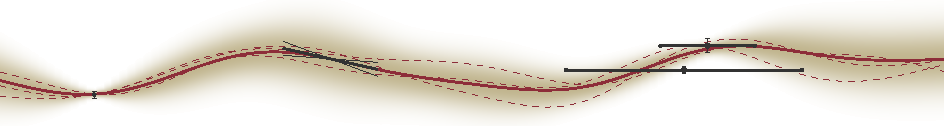
\includegraphics[width=0.9995\paperwidth]{assets/logo_TU_169_0.pdf}};
		\end{tikzpicture}%
	}%
	
\end{frame}
%\tikzexternalenable
\note[itemize]{
	\item Introduce myself, I study Cognitive Science
	\item I chose this topic because I wanted to get to know deep learning from the inside. I had never done Deep Learning before and wanted to learn it hands-on.
	\item In this talk I will talk about the science, but also about the process I used.
	\item If you have questions during the talk, ask them right away!
}


\setlength{\figwidth}{.9\textwidth}
\setlength{\figheight}{.6\textheight}

\section{Background}

\begin{frame}
\frametitle{Machine Learning}
\framesubtitle{Background}
	\begin{block}{Definition \footnote{Tom Mitchell, "Machine Learning", 1997}}
		"A computer program is said to learn from \emph{experience E} with respect to some class of \emph{tasks T} and \emph{performance measure P} if its performance at tasks in T, as measured by P, improves with experience E"
	\end{block}
\begin{itemize}
	\item Special case in Deep Learning: Finding the \emph{optimal point} in \emph{parameter space}
	\item The \emph{Loss function $\L (w)$} tells us how bad a specific parametrization $w$ is. For example, the model's predictions for all possible inputs are compared to the desired outputs.
	% TODO image of 2-dimensional problem
\end{itemize}
\end{frame}
\note[itemize]{
	\item Most of you will have seen this definition before.
	\item As an example, have a look at this 2-parametrical problem
}

\begin{frame}
\frametitle{Gradient Descent}
\framesubtitle{Optimization}
	Gradient Descent uses knowledge of the \emph{gradient} at a point in parameter space to take an update step:
		$$ w_{i+1} = w_i - \alpha \cdot \nabla \L(w_i) $$
	where $\alpha$ is the learning rate.
	
\end{frame}

\begin{frame}
\frametitle{Stochastic Gradient Descent}
\framesubtitle{Optimization}
\begin{itemize}
	\item In real life, we have Big Data. The true $\nabla \L(w)$ is expensive to compute.
	\item To speed things up, we compute the noisy estimate $\hat{\L}(w_i)$ on a minibatch of for example 128 data points.
\end{itemize}
The update rule still looks the same:
$$w_{i+1} = w_i - \alpha \cdot \nabla \hat{\L}(w_i) $$
where $\alpha$ is the learning rate.

\end{frame}


\begin{frame}
\frametitle{Preconditioning}
\framesubtitle{The condition number of the Hessian}
	\begin{itemize}
		\item The performance of (S)GD depends heavily on the shape of the loss landscape
		\item The \emph{condition number} is defined as $$\kappa = \frac{\lambda_n}{\lambda_1} > 1$$
			 where $\lambda_n, \lambda_1$ are the largest/smallest eigenvalues of the Hessian $\nabla \nabla \L(w)$
		\item For larger $\kappa$, (S)GD can converge slower.
		\item The condition number can be changed by carefully rescaling the gradient before taking the optimization step
		%TODO example image!
	\end{itemize}
\end{frame}

\begin{frame}{Probabilistic Preconditioning}{by Filip \& Philipp, 2019}
In the stochastic (minibatched) setting and while only having access to \emph{Hessian-vector products}, it isn't obvious how to construct the preconditioner. This is the method I'm testing:
\begin{enumerate}
	\item Empirically construct a prior for the multivariate Gaussian distribution and set the learning rate for SGD
	\item Gather observations and update the posterior estimate for the Hessian, using Bayes
	\item Create a rank-2 approximation of the Preconditioner
	\item apply the preconditioner at every step and do SGD
\end{enumerate}
\end{frame}
\note{If I'm grossly misrepresenting the algorithm, please correct me now! For an exact description check out the paper}

\begin{frame}{Deep learning}{Neural nets}
	For the purposes of this talk, a neural net is a model
	\begin{itemize}
		\item with many ( $>$ hundreds of thousands) parameters, weights $w$
		\item with an available noisy gradient $\nabla \hat\L(w_0)$, which was obtained by backpropagation
	\end{itemize}
\end{frame}

\section{Approach}
\begin{frame}{Evaluating an Optimizer}{Empirically}
	This is a hard problem in itself! How do you chose:
	\begin{itemize}
		\item Data Set
		\item Batch Size
		\item Model architecture
		\item Hyperparameter tuning method
		\item Measure of success
	\end{itemize}
	Comparing results between papers is very hard.
\end{frame}
\note{Now that we have roughly defined the algorithm, how do we test it?}

\begin{frame}{DeepOBS}{by Frank \& Aaron}
	\begin{itemize}
		\item A library for Tensorflow and Pytorch
		\item In order to test an optimizer, you have to specify only
			\begin{itemize}
			\item The optimizer class
			\item The hyperparameters of my optimizer
			\item One of the provided testproblems
			\end{itemize}
		\item DeepOBS then returns a json file
		\item And automatically generates figures
	\end{itemize}
\end{frame}

\begin{frame}[fragile]{Implementation Details}
	\framesubtitle{The class Preconditioner}
\begin{verbatim}
Preconditioner(params, est_rank=2, num_observations=5, prior_iterations=10,
               weight_decay=0, lr=None,
               optim_class=torch.optim.SGD, **optim_hyperparams)
start_estimate()
step()
get_log()
\end{verbatim}	
\end{frame}

\begin{frame}{How to use the TCML Cluster}{Cloud Computing}
\begin{enumerate}
	\item Request an account by sending an email
	\item If you have any special code requirements, build a Singularity container (kind of like a virtual machine). Alternatively use a provided one.
	\item Create \& Submit a Slurm Batch job file
	\item Get an e-mail when your jobs start of finish
	\item Download the output files to your local machine. You can mount the cluster as a virtual drive.
\end{enumerate}
\end{frame}
	

\section{Experiments + Results + Discussion}
\begin{frame}{Experiments}{Overview}
\begin{itemize}
	\item Effectiveness of Preconditioning
	\item Computational Complexity
	\item Stability
	\item Learning Rate sensitivity
\end{itemize}
\end{frame}

\begin{frame}{Effectiveness of Preconditioning}{\tikz\draw[orange,fill=orange] (0,0) circle (.7ex); AdaptiveSGD \hspace{1cm} \tikz\draw[white,fill=blue] (0,0) circle (.7ex); PreconditionedSGD}
\vspace{3mm}
% This file was created by tikzplotlib v0.8.2.
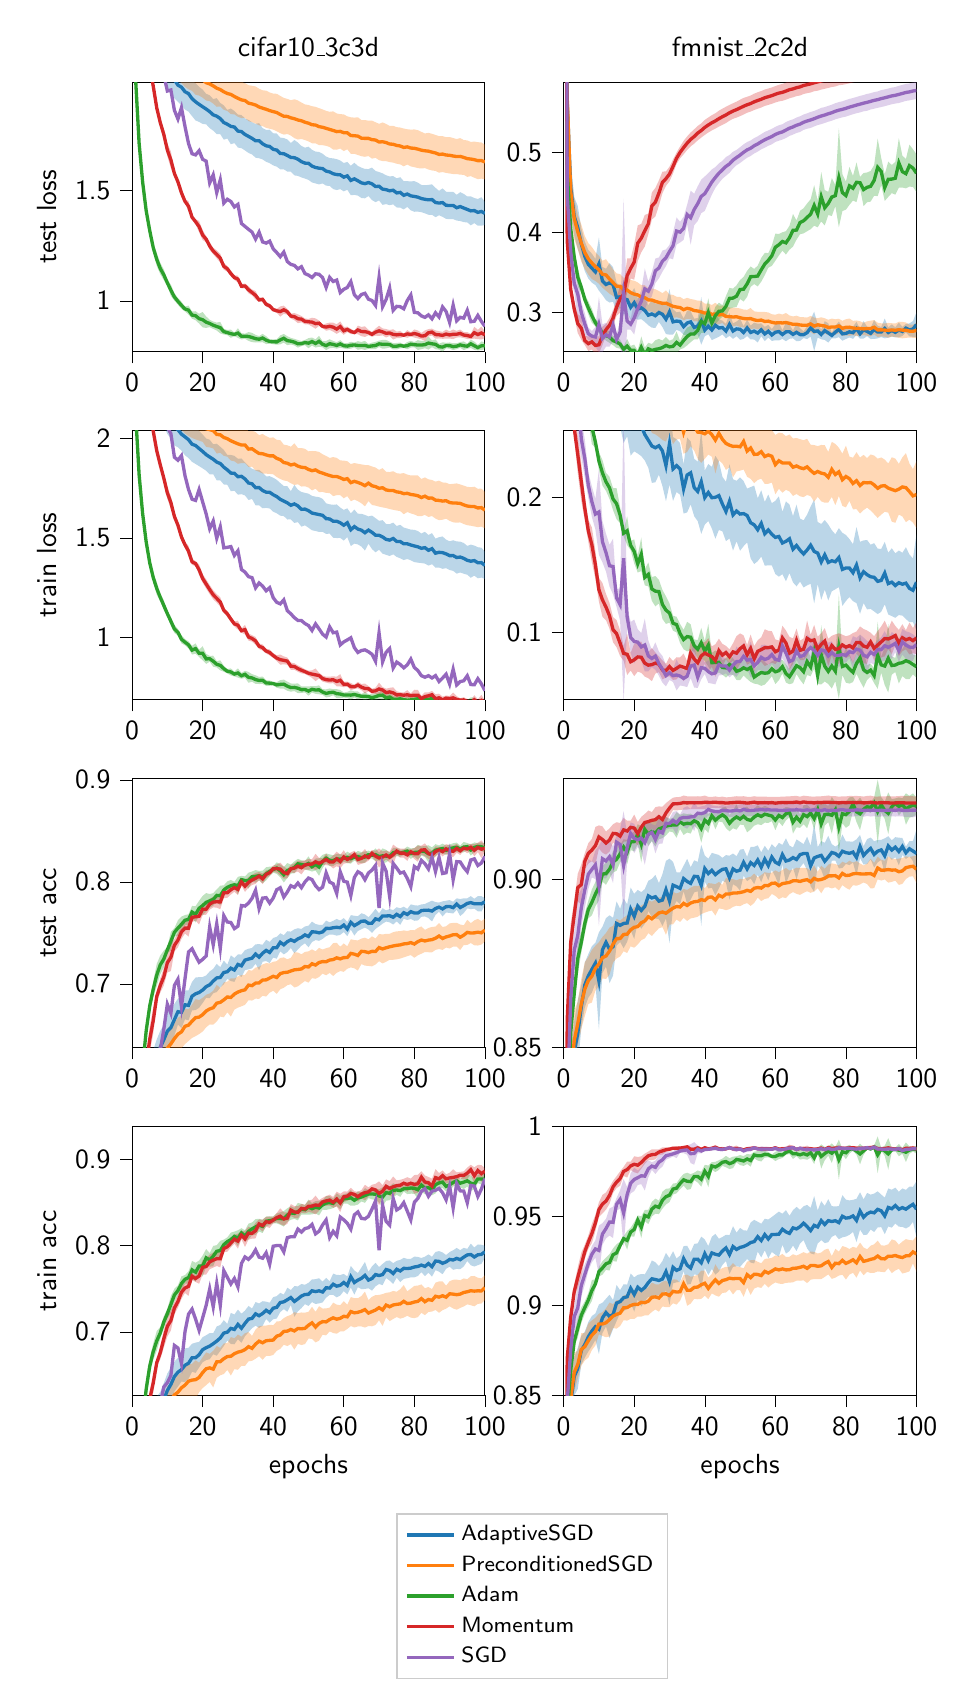
\begin{tikzpicture}

every axis plot post./append style={line width = 1pt}
\definecolor{color0}{rgb}{0.12156862745098,0.466666666666667,0.705882352941177}
\definecolor{color1}{rgb}{1,0.498039215686275,0.0549019607843137}
\definecolor{color2}{rgb}{0.172549019607843,0.627450980392157,0.172549019607843}
\definecolor{color3}{rgb}{0.83921568627451,0.152941176470588,0.156862745098039}
\definecolor{color4}{rgb}{0.580392156862745,0.403921568627451,0.741176470588235}

\begin{groupplot}[group style={group size=2 by 4}]
\nextgroupplot[
height=5cm,
legend style={font=\footnotesize, at={(0 ,0)},xshift=-0.4cm, yshift=-1.5cm,anchor=north,nodes=right},
tick align=outside,
tick pos=both,
tick pos=left,
title={cifar10\_3c3d},
width=\figurewidth,
x grid style={white!69.01960784313725!black},
xmin=0, xmax=100,
xtick style={color=black},
y grid style={white!69.01960784313725!black},
ylabel={test loss},
ymin=0.770326008810447, ymax=1.98583874852535,
ytick style={color=black}
]
\path [fill=color0, fill opacity=0.3]
(axis cs:0,3.5975588590671)
--(axis cs:0,3.57227203784844)
--(axis cs:1,2.73008363927707)
--(axis cs:2,2.44471123459844)
--(axis cs:3,2.31715896276543)
--(axis cs:4,2.19273855623163)
--(axis cs:5,2.14686945963002)
--(axis cs:6,2.08868770887586)
--(axis cs:7,2.04893022510944)
--(axis cs:8,2.01929264668992)
--(axis cs:9,1.9906933791226)
--(axis cs:10,1.95866343396377)
--(axis cs:11,1.94098673792146)
--(axis cs:12,1.9143659119725)
--(axis cs:13,1.89916684324181)
--(axis cs:14,1.88301045905781)
--(axis cs:15,1.86353390435769)
--(axis cs:16,1.85437520445145)
--(axis cs:17,1.83366706361729)
--(axis cs:18,1.81440797513137)
--(axis cs:19,1.80786767518252)
--(axis cs:20,1.79881377915512)
--(axis cs:21,1.79682097144257)
--(axis cs:22,1.77989208056918)
--(axis cs:23,1.76820745277051)
--(axis cs:24,1.75241603052307)
--(axis cs:25,1.75222295888863)
--(axis cs:26,1.72749600050764)
--(axis cs:27,1.73266690126953)
--(axis cs:28,1.70676903006441)
--(axis cs:29,1.71239953470703)
--(axis cs:30,1.69198979808297)
--(axis cs:31,1.68928186557013)
--(axis cs:32,1.67911532471683)
--(axis cs:33,1.66777070509495)
--(axis cs:34,1.6609006451075)
--(axis cs:35,1.64620687650848)
--(axis cs:36,1.64375724535349)
--(axis cs:37,1.63829379294225)
--(axis cs:38,1.62786656171001)
--(axis cs:39,1.6214171392674)
--(axis cs:40,1.61151956866956)
--(axis cs:41,1.6058889442369)
--(axis cs:42,1.59372189980484)
--(axis cs:43,1.59379414759487)
--(axis cs:44,1.58361435354524)
--(axis cs:45,1.58284285515073)
--(axis cs:46,1.56643918715507)
--(axis cs:47,1.56401234383455)
--(axis cs:48,1.55727099359894)
--(axis cs:49,1.55200929900525)
--(axis cs:50,1.5460541738488)
--(axis cs:51,1.53444292290378)
--(axis cs:52,1.53009435448683)
--(axis cs:53,1.52551828213507)
--(axis cs:54,1.53009202320624)
--(axis cs:55,1.51988758148204)
--(axis cs:56,1.51904759686098)
--(axis cs:57,1.50454361627299)
--(axis cs:58,1.50016058719833)
--(axis cs:59,1.50417036914587)
--(axis cs:60,1.4943673821255)
--(axis cs:61,1.5013813759504)
--(axis cs:62,1.47686013875744)
--(axis cs:63,1.47816760934225)
--(axis cs:64,1.47496158668577)
--(axis cs:65,1.46413720370549)
--(axis cs:66,1.462756180028)
--(axis cs:67,1.47307474909779)
--(axis cs:68,1.45481660566145)
--(axis cs:69,1.44573303321513)
--(axis cs:70,1.45300705990818)
--(axis cs:71,1.43320106067667)
--(axis cs:72,1.43662936901701)
--(axis cs:73,1.43180597629963)
--(axis cs:74,1.43538272840375)
--(axis cs:75,1.42144355549492)
--(axis cs:76,1.42090662887148)
--(axis cs:77,1.41270213952912)
--(axis cs:78,1.42399658191475)
--(axis cs:79,1.40855605746742)
--(axis cs:80,1.40203126303114)
--(axis cs:81,1.40276371264279)
--(axis cs:82,1.40031943350696)
--(axis cs:83,1.39501728851651)
--(axis cs:84,1.38862803680633)
--(axis cs:85,1.38835011127894)
--(axis cs:86,1.37768692081291)
--(axis cs:87,1.3861188902397)
--(axis cs:88,1.37927013264026)
--(axis cs:89,1.36995109804743)
--(axis cs:90,1.36856998605876)
--(axis cs:91,1.3689294097774)
--(axis cs:92,1.36233279568516)
--(axis cs:93,1.36041210512546)
--(axis cs:94,1.35518848361032)
--(axis cs:95,1.35397069379817)
--(axis cs:96,1.34087564126939)
--(axis cs:97,1.35082025906634)
--(axis cs:98,1.33893840847823)
--(axis cs:99,1.3392335633384)
--(axis cs:100,1.3424614994151)
--(axis cs:100,1.44712457114692)
--(axis cs:100,1.44712457114692)
--(axis cs:99,1.46758989126782)
--(axis cs:98,1.45962756062214)
--(axis cs:97,1.46424514379601)
--(axis cs:96,1.47148449566749)
--(axis cs:95,1.47140805398294)
--(axis cs:94,1.48283565151467)
--(axis cs:93,1.49065153089627)
--(axis cs:92,1.47855429663619)
--(axis cs:91,1.49244507326998)
--(axis cs:90,1.49196619342265)
--(axis cs:89,1.49251245600478)
--(axis cs:88,1.5077261280272)
--(axis cs:87,1.4966522835676)
--(axis cs:86,1.51013883263137)
--(axis cs:85,1.52608870432701)
--(axis cs:84,1.52341683160178)
--(axis cs:83,1.52178160326014)
--(axis cs:82,1.52311962416109)
--(axis cs:81,1.5335065087373)
--(axis cs:80,1.54052243048346)
--(axis cs:79,1.53920716666971)
--(axis cs:78,1.54022126949174)
--(axis cs:77,1.54037927755462)
--(axis cs:76,1.55820950833966)
--(axis cs:75,1.55307764803522)
--(axis cs:74,1.56323026448203)
--(axis cs:73,1.56166281968459)
--(axis cs:72,1.56690502319314)
--(axis cs:71,1.57547563147902)
--(axis cs:70,1.58150744736106)
--(axis cs:69,1.5863770067893)
--(axis cs:68,1.60147873849564)
--(axis cs:67,1.59498762543291)
--(axis cs:66,1.59551915401233)
--(axis cs:65,1.60122734111407)
--(axis cs:64,1.60895369674966)
--(axis cs:63,1.62345199985473)
--(axis cs:62,1.61021334446513)
--(axis cs:61,1.6269447707745)
--(axis cs:60,1.62230273488593)
--(axis cs:59,1.6335729379311)
--(axis cs:58,1.63986746861627)
--(axis cs:57,1.64314655977382)
--(axis cs:56,1.64484996638865)
--(axis cs:55,1.65128725498238)
--(axis cs:54,1.66415129203809)
--(axis cs:53,1.67219087203063)
--(axis cs:52,1.67378929220921)
--(axis cs:51,1.68209422286979)
--(axis cs:50,1.69580893047016)
--(axis cs:49,1.69159376973775)
--(axis cs:48,1.69940751213964)
--(axis cs:47,1.71479083597971)
--(axis cs:46,1.72621711590834)
--(axis cs:45,1.7124733650961)
--(axis cs:44,1.72874312319049)
--(axis cs:43,1.73488986358326)
--(axis cs:42,1.73696781622861)
--(axis cs:41,1.75543892278197)
--(axis cs:40,1.75669517245041)
--(axis cs:39,1.77257830838048)
--(axis cs:38,1.77198949826916)
--(axis cs:37,1.779738788436)
--(axis cs:36,1.80235565454905)
--(axis cs:35,1.79894170980139)
--(axis cs:34,1.80636962893253)
--(axis cs:33,1.81706001306778)
--(axis cs:32,1.82349323160268)
--(axis cs:31,1.83919398479191)
--(axis cs:30,1.84087646469529)
--(axis cs:29,1.85710341195098)
--(axis cs:28,1.86852688774002)
--(axis cs:27,1.86200673108325)
--(axis cs:26,1.88257548129488)
--(axis cs:25,1.89325481592705)
--(axis cs:24,1.91506465830562)
--(axis cs:23,1.91102274480586)
--(axis cs:22,1.92851115800854)
--(axis cs:21,1.93484430909516)
--(axis cs:20,1.9537281333639)
--(axis cs:19,1.96641605305023)
--(axis cs:18,1.98294247858774)
--(axis cs:17,1.99207260006922)
--(axis cs:16,2.01687004068735)
--(axis cs:15,2.02474518581452)
--(axis cs:14,2.04628161700412)
--(axis cs:13,2.04876759905825)
--(axis cs:12,2.0810666785488)
--(axis cs:11,2.10487456985849)
--(axis cs:10,2.12322382619203)
--(axis cs:9,2.14625435877904)
--(axis cs:8,2.17423842667248)
--(axis cs:7,2.20051522641916)
--(axis cs:6,2.27058768503809)
--(axis cs:5,2.26674769066446)
--(axis cs:4,2.34305969356326)
--(axis cs:3,2.40518698056323)
--(axis cs:2,2.59165202840949)
--(axis cs:1,2.84845361028805)
--(axis cs:0,3.5975588590671)
--cycle;

\path [fill=color1, fill opacity=0.3]
(axis cs:0,3.5975588590671)
--(axis cs:0,3.57227203784844)
--(axis cs:1,2.73856869377099)
--(axis cs:2,2.42288736776192)
--(axis cs:3,2.29844370590286)
--(axis cs:4,2.21789891356138)
--(axis cs:5,2.17524797367773)
--(axis cs:6,2.13580789735739)
--(axis cs:7,2.1063757028166)
--(axis cs:8,2.08299618943434)
--(axis cs:9,2.06552463318946)
--(axis cs:10,2.03930346238643)
--(axis cs:11,2.02522969128598)
--(axis cs:12,2.01097521418159)
--(axis cs:13,1.99574155680415)
--(axis cs:14,1.98311257512216)
--(axis cs:15,1.96629865246767)
--(axis cs:16,1.95550138250703)
--(axis cs:17,1.9479444402456)
--(axis cs:18,1.9306450438284)
--(axis cs:19,1.92672807628384)
--(axis cs:20,1.91732555628161)
--(axis cs:21,1.90443211799475)
--(axis cs:22,1.9016270273367)
--(axis cs:23,1.89038829762654)
--(axis cs:24,1.87619574041118)
--(axis cs:25,1.87760149897918)
--(axis cs:26,1.86255474893484)
--(axis cs:27,1.8573793804416)
--(axis cs:28,1.84275147939657)
--(axis cs:29,1.84210570394026)
--(axis cs:30,1.83115017567738)
--(axis cs:31,1.8250736479494)
--(axis cs:32,1.82596315171712)
--(axis cs:33,1.8112461781729)
--(axis cs:34,1.80691898092972)
--(axis cs:35,1.8001442108556)
--(axis cs:36,1.79247497418431)
--(axis cs:37,1.78891319382367)
--(axis cs:38,1.78098847092835)
--(axis cs:39,1.77701648048734)
--(axis cs:40,1.77298175691627)
--(axis cs:41,1.76561336513282)
--(axis cs:42,1.75694943287532)
--(axis cs:43,1.75049814942373)
--(axis cs:44,1.7534191302113)
--(axis cs:45,1.7462708915332)
--(axis cs:46,1.73456244881257)
--(axis cs:47,1.72832829179254)
--(axis cs:48,1.73069798830553)
--(axis cs:49,1.72590743542004)
--(axis cs:50,1.71989033841309)
--(axis cs:51,1.71139476308167)
--(axis cs:52,1.71139570585275)
--(axis cs:53,1.70305749226927)
--(axis cs:54,1.70272967461413)
--(axis cs:55,1.69985753177754)
--(axis cs:56,1.69432416388791)
--(axis cs:57,1.6829046834126)
--(axis cs:58,1.6821057225632)
--(axis cs:59,1.68750168534938)
--(axis cs:60,1.6762783022834)
--(axis cs:61,1.68401124266759)
--(axis cs:62,1.66383327549528)
--(axis cs:63,1.66374297739986)
--(axis cs:64,1.65839525152034)
--(axis cs:65,1.65288848812932)
--(axis cs:66,1.65029658121562)
--(axis cs:67,1.65351397761111)
--(axis cs:68,1.64188593048243)
--(axis cs:69,1.64567260683282)
--(axis cs:70,1.63502737167614)
--(axis cs:71,1.63104430169096)
--(axis cs:72,1.63050758928941)
--(axis cs:73,1.62635838435753)
--(axis cs:74,1.62398684866506)
--(axis cs:75,1.61899904474547)
--(axis cs:76,1.61588035421757)
--(axis cs:77,1.60732985989665)
--(axis cs:78,1.61554529244745)
--(axis cs:79,1.60674871298736)
--(axis cs:80,1.60353555999171)
--(axis cs:81,1.59929240789746)
--(axis cs:82,1.59749562354027)
--(axis cs:83,1.59925073141487)
--(axis cs:84,1.59296482219767)
--(axis cs:85,1.58859688801748)
--(axis cs:86,1.58641574373291)
--(axis cs:87,1.57876053194559)
--(axis cs:88,1.58147623665886)
--(axis cs:89,1.57751839442663)
--(axis cs:90,1.57485119812859)
--(axis cs:91,1.57252179405166)
--(axis cs:92,1.57247256136123)
--(axis cs:93,1.56947237511914)
--(axis cs:94,1.56901425087068)
--(axis cs:95,1.55958508496522)
--(axis cs:96,1.56303617171352)
--(axis cs:97,1.55564958762106)
--(axis cs:98,1.54929719918812)
--(axis cs:99,1.55178583667416)
--(axis cs:100,1.54814573985329)
--(axis cs:100,1.7051951350265)
--(axis cs:100,1.7051951350265)
--(axis cs:99,1.71502625065385)
--(axis cs:98,1.71624855200451)
--(axis cs:97,1.71901358530865)
--(axis cs:96,1.71737000227374)
--(axis cs:95,1.7242964402334)
--(axis cs:94,1.72608907228328)
--(axis cs:93,1.73468603248342)
--(axis cs:92,1.7305261119433)
--(axis cs:91,1.73515167215394)
--(axis cs:90,1.73952459488829)
--(axis cs:89,1.73899974724653)
--(axis cs:88,1.74357393975378)
--(axis cs:87,1.74345579023191)
--(axis cs:86,1.74878104170484)
--(axis cs:85,1.75422075259275)
--(axis cs:84,1.75852230360254)
--(axis cs:83,1.75572577928105)
--(axis cs:82,1.76288874963552)
--(axis cs:81,1.77067494850315)
--(axis cs:80,1.77387162555057)
--(axis cs:79,1.77292950335997)
--(axis cs:78,1.77475570954147)
--(axis cs:77,1.77783837491626)
--(axis cs:76,1.78237164451263)
--(axis cs:75,1.78430168197392)
--(axis cs:74,1.79013506371653)
--(axis cs:73,1.7895457542809)
--(axis cs:72,1.79870217367508)
--(axis cs:71,1.80549689493653)
--(axis cs:70,1.79900089098797)
--(axis cs:69,1.80655250241424)
--(axis cs:68,1.81344103382257)
--(axis cs:67,1.81318213588973)
--(axis cs:66,1.81639856424466)
--(axis cs:65,1.81638923427829)
--(axis cs:64,1.8288142678415)
--(axis cs:63,1.82723970334881)
--(axis cs:62,1.82880334855975)
--(axis cs:61,1.83281423339195)
--(axis cs:60,1.84207565908653)
--(axis cs:59,1.8427791211187)
--(axis cs:58,1.8460195409199)
--(axis cs:57,1.85543774479479)
--(axis cs:56,1.85351636258286)
--(axis cs:55,1.85778680365133)
--(axis cs:54,1.864431963389)
--(axis cs:53,1.86991793296188)
--(axis cs:52,1.87583517061748)
--(axis cs:51,1.87892502873661)
--(axis cs:50,1.88408414759558)
--(axis cs:49,1.8868861694185)
--(axis cs:48,1.89538433300818)
--(axis cs:47,1.90470103187093)
--(axis cs:46,1.91005176229434)
--(axis cs:45,1.9060039020061)
--(axis cs:44,1.91173784158566)
--(axis cs:43,1.91628403410116)
--(axis cs:42,1.9254702578437)
--(axis cs:41,1.93479708742868)
--(axis cs:40,1.9356298402427)
--(axis cs:39,1.94080621643075)
--(axis cs:38,1.94887138063983)
--(axis cs:37,1.95068230955546)
--(axis cs:36,1.95775650091218)
--(axis cs:35,1.9681630519563)
--(axis cs:34,1.97099839744698)
--(axis cs:33,1.97387528441675)
--(axis cs:32,1.98286352345339)
--(axis cs:31,1.98957556288266)
--(axis cs:30,1.99776673744074)
--(axis cs:29,2.00319172678288)
--(axis cs:28,2.02126099213259)
--(axis cs:27,2.01493987712344)
--(axis cs:26,2.02508427905193)
--(axis cs:25,2.03034115555714)
--(axis cs:24,2.04392088986181)
--(axis cs:23,2.0506003393073)
--(axis cs:22,2.05725902689792)
--(axis cs:21,2.06527705614921)
--(axis cs:20,2.07893681709245)
--(axis cs:19,2.08884620505409)
--(axis cs:18,2.09677872219773)
--(axis cs:17,2.10863800511913)
--(axis cs:16,2.11562342701486)
--(axis cs:15,2.12945005113437)
--(axis cs:14,2.14190762962976)
--(axis cs:13,2.15163400055736)
--(axis cs:12,2.1647587598595)
--(axis cs:11,2.18365490676132)
--(axis cs:10,2.20324913134606)
--(axis cs:9,2.21250527356026)
--(axis cs:8,2.23432369217604)
--(axis cs:7,2.25215692185603)
--(axis cs:6,2.27601406801914)
--(axis cs:5,2.30378861364617)
--(axis cs:4,2.35071259489365)
--(axis cs:3,2.40866104365444)
--(axis cs:2,2.5425748632628)
--(axis cs:1,2.86009621170375)
--(axis cs:0,3.5975588590671)
--cycle;

\path [fill=color2, fill opacity=0.3]
(axis cs:0,3.59755885070715)
--(axis cs:0,3.57227203459312)
--(axis cs:1,1.9796592054112)
--(axis cs:2,1.68088429923241)
--(axis cs:3,1.5069366828042)
--(axis cs:4,1.38472368631195)
--(axis cs:5,1.29188547798051)
--(axis cs:6,1.21796735152716)
--(axis cs:7,1.15737591531276)
--(axis cs:8,1.12011975418557)
--(axis cs:9,1.09328394852482)
--(axis cs:10,1.06822164010733)
--(axis cs:11,1.02206758267732)
--(axis cs:12,1.00035211789025)
--(axis cs:13,0.982684253991911)
--(axis cs:14,0.963113955701856)
--(axis cs:15,0.95206781884604)
--(axis cs:16,0.937664848980681)
--(axis cs:17,0.919329134742481)
--(axis cs:18,0.912234822177166)
--(axis cs:19,0.897200591301827)
--(axis cs:20,0.880053583987961)
--(axis cs:21,0.877455626521624)
--(axis cs:22,0.881253847416339)
--(axis cs:23,0.873161355753856)
--(axis cs:24,0.865910244976317)
--(axis cs:25,0.852600076471727)
--(axis cs:26,0.847834600113664)
--(axis cs:27,0.844854806553819)
--(axis cs:28,0.832964344634736)
--(axis cs:29,0.840326512163106)
--(axis cs:30,0.832270870522744)
--(axis cs:31,0.825564307261934)
--(axis cs:32,0.828991510615148)
--(axis cs:33,0.818905292608983)
--(axis cs:34,0.813453919994327)
--(axis cs:35,0.811712086507817)
--(axis cs:36,0.812303779688529)
--(axis cs:37,0.813142193087901)
--(axis cs:38,0.80450662044439)
--(axis cs:39,0.806538331932455)
--(axis cs:40,0.804119376013852)
--(axis cs:41,0.801667271304423)
--(axis cs:42,0.803676952627977)
--(axis cs:43,0.810919018532278)
--(axis cs:44,0.799721907402972)
--(axis cs:45,0.802879456305825)
--(axis cs:46,0.798437359914708)
--(axis cs:47,0.788594660668623)
--(axis cs:48,0.795442072086427)
--(axis cs:49,0.799585411925887)
--(axis cs:50,0.785977948757053)
--(axis cs:51,0.797857723170871)
--(axis cs:52,0.788993981863456)
--(axis cs:53,0.792611672817111)
--(axis cs:54,0.789785930394425)
--(axis cs:55,0.77724061386981)
--(axis cs:56,0.786134597532406)
--(axis cs:57,0.78756742782573)
--(axis cs:58,0.783980298207806)
--(axis cs:59,0.788305359307613)
--(axis cs:60,0.784745176205981)
--(axis cs:61,0.782096924230827)
--(axis cs:62,0.783806318910576)
--(axis cs:63,0.78951603452262)
--(axis cs:64,0.778818488166703)
--(axis cs:65,0.782086859487721)
--(axis cs:66,0.778189335096993)
--(axis cs:67,0.782700354876578)
--(axis cs:68,0.781534128470355)
--(axis cs:69,0.781663148240256)
--(axis cs:70,0.791135589642423)
--(axis cs:71,0.783673106337051)
--(axis cs:72,0.785002424647669)
--(axis cs:73,0.789273485995176)
--(axis cs:74,0.780130754344501)
--(axis cs:75,0.780348670184861)
--(axis cs:76,0.785370298067026)
--(axis cs:77,0.78695915151653)
--(axis cs:78,0.781271676973452)
--(axis cs:79,0.788911927800886)
--(axis cs:80,0.790128138261899)
--(axis cs:81,0.777824335297643)
--(axis cs:82,0.781482221380957)
--(axis cs:83,0.785891824545463)
--(axis cs:84,0.779676919480312)
--(axis cs:85,0.790642892234378)
--(axis cs:86,0.78134081590102)
--(axis cs:87,0.779560392893656)
--(axis cs:88,0.76946066590553)
--(axis cs:89,0.785434647620617)
--(axis cs:90,0.783611827109979)
--(axis cs:91,0.777651618885547)
--(axis cs:92,0.781911844581631)
--(axis cs:93,0.787913194565458)
--(axis cs:94,0.77742263694221)
--(axis cs:95,0.783466342430419)
--(axis cs:96,0.787251167208227)
--(axis cs:97,0.778308612137632)
--(axis cs:98,0.776527439047234)
--(axis cs:99,0.777026074844734)
--(axis cs:100,0.782398138996916)
--(axis cs:100,0.810877622913058)
--(axis cs:100,0.810877622913058)
--(axis cs:99,0.816645898854444)
--(axis cs:98,0.800956124345357)
--(axis cs:97,0.815778635527479)
--(axis cs:96,0.82460955677632)
--(axis cs:95,0.806727088763593)
--(axis cs:94,0.816419155891901)
--(axis cs:93,0.813921498145027)
--(axis cs:92,0.808486961140581)
--(axis cs:91,0.808479671403525)
--(axis cs:90,0.811871484060208)
--(axis cs:89,0.810186960233199)
--(axis cs:88,0.812766490959761)
--(axis cs:87,0.806090534393226)
--(axis cs:86,0.82597968443614)
--(axis cs:85,0.820848812669739)
--(axis cs:84,0.838768518207781)
--(axis cs:83,0.818220633836434)
--(axis cs:82,0.818853959437429)
--(axis cs:81,0.822290390041464)
--(axis cs:80,0.813885707597531)
--(axis cs:79,0.819351138686548)
--(axis cs:78,0.81373251876561)
--(axis cs:77,0.803412659567729)
--(axis cs:76,0.81155269895526)
--(axis cs:75,0.809820823172479)
--(axis cs:74,0.808691230979723)
--(axis cs:73,0.815754043831355)
--(axis cs:72,0.8231919075974)
--(axis cs:71,0.823474792398093)
--(axis cs:70,0.820197421257292)
--(axis cs:69,0.814451786320324)
--(axis cs:68,0.811091513505292)
--(axis cs:67,0.805461680026239)
--(axis cs:66,0.819037023432856)
--(axis cs:65,0.814155074995147)
--(axis cs:64,0.817738247483384)
--(axis cs:63,0.811557186842991)
--(axis cs:62,0.81492478867895)
--(axis cs:61,0.808739342598591)
--(axis cs:60,0.809566611020281)
--(axis cs:59,0.822109086092625)
--(axis cs:58,0.812954483569747)
--(axis cs:57,0.818724577707097)
--(axis cs:56,0.826408198602542)
--(axis cs:55,0.818360044938189)
--(axis cs:54,0.8171888189873)
--(axis cs:53,0.841438440298444)
--(axis cs:52,0.825721353903018)
--(axis cs:51,0.834132301200153)
--(axis cs:50,0.831465899663359)
--(axis cs:49,0.823403989830301)
--(axis cs:48,0.817996990533393)
--(axis cs:47,0.822929998573762)
--(axis cs:46,0.828431258078427)
--(axis cs:45,0.832624375276367)
--(axis cs:44,0.84014890524541)
--(axis cs:43,0.850537107289545)
--(axis cs:42,0.843533799571881)
--(axis cs:41,0.826807254153351)
--(axis cs:40,0.826127580212302)
--(axis cs:39,0.826150250622387)
--(axis cs:38,0.840228123328019)
--(axis cs:37,0.850785788093121)
--(axis cs:36,0.840614137575285)
--(axis cs:35,0.846319182559556)
--(axis cs:34,0.85537136861931)
--(axis cs:33,0.858939352512176)
--(axis cs:32,0.851670145844024)
--(axis cs:31,0.85393679113246)
--(axis cs:30,0.876180977935277)
--(axis cs:29,0.856226956235453)
--(axis cs:28,0.870142915953152)
--(axis cs:27,0.868038511353465)
--(axis cs:26,0.873669133710797)
--(axis cs:25,0.904911762416784)
--(axis cs:24,0.901685246066187)
--(axis cs:23,0.906450936939356)
--(axis cs:22,0.913971336364038)
--(axis cs:21,0.929409719757276)
--(axis cs:20,0.949255390296431)
--(axis cs:19,0.941451669796398)
--(axis cs:18,0.952870203102051)
--(axis cs:17,0.951690742941941)
--(axis cs:16,0.97806446510814)
--(axis cs:15,0.974747580910759)
--(axis cs:14,0.995842220035035)
--(axis cs:13,1.01281162183739)
--(axis cs:12,1.03454245365861)
--(axis cs:11,1.07319595088433)
--(axis cs:10,1.09422394008783)
--(axis cs:9,1.14162920622395)
--(axis cs:8,1.17123142051133)
--(axis cs:7,1.21587215776383)
--(axis cs:6,1.26192183744717)
--(axis cs:5,1.34300400424867)
--(axis cs:4,1.42877022603031)
--(axis cs:3,1.56411876036043)
--(axis cs:2,1.74040984433431)
--(axis cs:1,2.02292255052036)
--(axis cs:0,3.59755885070715)
--cycle;

\path [fill=color3, fill opacity=0.3]
(axis cs:0,3.59755886207645)
--(axis cs:0,3.57227203117111)
--(axis cs:1,2.73211047815408)
--(axis cs:2,2.45742197522946)
--(axis cs:3,2.27789487459308)
--(axis cs:4,2.1391180824476)
--(axis cs:5,2.02676995156382)
--(axis cs:6,1.93265703316272)
--(axis cs:7,1.85581215410196)
--(axis cs:8,1.78780676594999)
--(axis cs:9,1.72481662503516)
--(axis cs:10,1.65240489974452)
--(axis cs:11,1.5984308931649)
--(axis cs:12,1.56189776719371)
--(axis cs:13,1.52147616011345)
--(axis cs:14,1.46737869773148)
--(axis cs:15,1.44051293926352)
--(axis cs:16,1.40380630172741)
--(axis cs:17,1.36846520146146)
--(axis cs:18,1.3456800655873)
--(axis cs:19,1.30946952522606)
--(axis cs:20,1.27444524433242)
--(axis cs:21,1.26463909712689)
--(axis cs:22,1.22934875984106)
--(axis cs:23,1.21050355708615)
--(axis cs:24,1.19140221794545)
--(axis cs:25,1.17281342767128)
--(axis cs:26,1.14027970301245)
--(axis cs:27,1.13189956821241)
--(axis cs:28,1.11029967417594)
--(axis cs:29,1.09424689470542)
--(axis cs:30,1.08282717293488)
--(axis cs:31,1.05664987036762)
--(axis cs:32,1.05585697211122)
--(axis cs:33,1.03394526392674)
--(axis cs:34,1.0243431205323)
--(axis cs:35,1.00579159634072)
--(axis cs:36,0.995358526411045)
--(axis cs:37,0.997314062982015)
--(axis cs:38,0.973508257312501)
--(axis cs:39,0.967262356867463)
--(axis cs:40,0.95095444103179)
--(axis cs:41,0.946052280140712)
--(axis cs:42,0.928522323616315)
--(axis cs:43,0.941070598580947)
--(axis cs:44,0.93774838149501)
--(axis cs:45,0.920383449338723)
--(axis cs:46,0.912483413504511)
--(axis cs:47,0.898863632200342)
--(axis cs:48,0.903129510938699)
--(axis cs:49,0.893846569057106)
--(axis cs:50,0.892964615862776)
--(axis cs:51,0.883849130108953)
--(axis cs:52,0.873748939856305)
--(axis cs:53,0.886951735187868)
--(axis cs:54,0.876944247684692)
--(axis cs:55,0.865104024287616)
--(axis cs:56,0.868379989610852)
--(axis cs:57,0.860772168475795)
--(axis cs:58,0.850649274940192)
--(axis cs:59,0.860503000127929)
--(axis cs:60,0.846658458207829)
--(axis cs:61,0.859150434302838)
--(axis cs:62,0.849601093370758)
--(axis cs:63,0.849460504649669)
--(axis cs:64,0.848920857255861)
--(axis cs:65,0.840298165873214)
--(axis cs:66,0.836795961969101)
--(axis cs:67,0.844501473992429)
--(axis cs:68,0.837703473656976)
--(axis cs:69,0.842547115102637)
--(axis cs:70,0.841401042752011)
--(axis cs:71,0.843798496435193)
--(axis cs:72,0.834386075387506)
--(axis cs:73,0.8412431361123)
--(axis cs:74,0.82526615456624)
--(axis cs:75,0.831539105901959)
--(axis cs:76,0.831801606902337)
--(axis cs:77,0.837129577313249)
--(axis cs:78,0.832928118579945)
--(axis cs:79,0.839252330102288)
--(axis cs:80,0.834031773104631)
--(axis cs:81,0.829958985000953)
--(axis cs:82,0.82657479649898)
--(axis cs:83,0.818454393267634)
--(axis cs:84,0.839151472838925)
--(axis cs:85,0.84334759529204)
--(axis cs:86,0.828882910803621)
--(axis cs:87,0.830015067518171)
--(axis cs:88,0.828404489827521)
--(axis cs:89,0.8292486531192)
--(axis cs:90,0.829460707472339)
--(axis cs:91,0.827138074421759)
--(axis cs:92,0.834087154325418)
--(axis cs:93,0.835202308531856)
--(axis cs:94,0.831946810069308)
--(axis cs:95,0.827431686571207)
--(axis cs:96,0.826864846448417)
--(axis cs:97,0.829235595033985)
--(axis cs:98,0.826687482993873)
--(axis cs:99,0.825839908414807)
--(axis cs:100,0.831134534694387)
--(axis cs:100,0.862002815754809)
--(axis cs:100,0.862002815754809)
--(axis cs:99,0.88376338226532)
--(axis cs:98,0.868799207912505)
--(axis cs:97,0.882708215227228)
--(axis cs:96,0.851142498109272)
--(axis cs:95,0.858562033141075)
--(axis cs:94,0.858901690842698)
--(axis cs:93,0.87010083531177)
--(axis cs:92,0.864112398277839)
--(axis cs:91,0.870589803396862)
--(axis cs:90,0.862149638306982)
--(axis cs:89,0.870045045747962)
--(axis cs:88,0.859506842131739)
--(axis cs:87,0.8629145858085)
--(axis cs:86,0.866271801946741)
--(axis cs:85,0.874246538445719)
--(axis cs:84,0.872251161787855)
--(axis cs:83,0.866174740610976)
--(axis cs:82,0.855137972587565)
--(axis cs:81,0.866211218807074)
--(axis cs:80,0.870686709542556)
--(axis cs:79,0.856972794342429)
--(axis cs:78,0.86798476185908)
--(axis cs:77,0.8518767705264)
--(axis cs:76,0.864163942676697)
--(axis cs:75,0.860790181321368)
--(axis cs:74,0.871491512467861)
--(axis cs:73,0.868060721617685)
--(axis cs:72,0.87239242967494)
--(axis cs:71,0.875319024276168)
--(axis cs:70,0.887497442443931)
--(axis cs:69,0.874644979039983)
--(axis cs:68,0.859525233601542)
--(axis cs:67,0.869169415544111)
--(axis cs:66,0.884801210236164)
--(axis cs:65,0.881836980127232)
--(axis cs:64,0.887896758968428)
--(axis cs:63,0.864008707222138)
--(axis cs:62,0.873915218947213)
--(axis cs:61,0.882893467562461)
--(axis cs:60,0.882691342201586)
--(axis cs:59,0.906827444189669)
--(axis cs:58,0.893910001622279)
--(axis cs:57,0.901193637427664)
--(axis cs:56,0.901361705132965)
--(axis cs:55,0.897681949016741)
--(axis cs:54,0.891177138959475)
--(axis cs:53,0.91089328363913)
--(axis cs:52,0.920557054409813)
--(axis cs:51,0.923565746083091)
--(axis cs:50,0.917717480374015)
--(axis cs:49,0.920451930184748)
--(axis cs:48,0.931322953397305)
--(axis cs:47,0.938903899732587)
--(axis cs:46,0.944591385177286)
--(axis cs:45,0.941665603009781)
--(axis cs:44,0.963930515983631)
--(axis cs:43,0.977989889655309)
--(axis cs:42,0.974549779095436)
--(axis cs:41,0.963490935934941)
--(axis cs:40,0.969285512473897)
--(axis cs:39,0.987110210529435)
--(axis cs:38,0.994761590594052)
--(axis cs:37,1.0156752954309)
--(axis cs:36,1.01310622691107)
--(axis cs:35,1.0439875896941)
--(axis cs:34,1.05100313966077)
--(axis cs:33,1.06602603093483)
--(axis cs:32,1.07817744404472)
--(axis cs:31,1.07527588628858)
--(axis cs:30,1.11329311824928)
--(axis cs:29,1.11581149103965)
--(axis cs:28,1.13547039814974)
--(axis cs:27,1.15774566500302)
--(axis cs:26,1.17109874924578)
--(axis cs:25,1.21240804004988)
--(axis cs:24,1.22773059349695)
--(axis cs:23,1.23948012285645)
--(axis cs:22,1.26508654960572)
--(axis cs:21,1.29190675281994)
--(axis cs:20,1.31946162042072)
--(axis cs:19,1.36034500486535)
--(axis cs:18,1.36866017983076)
--(axis cs:17,1.3862503387031)
--(axis cs:16,1.45024860561897)
--(axis cs:15,1.45792047735981)
--(axis cs:14,1.50799488645341)
--(axis cs:13,1.55290161232782)
--(axis cs:12,1.58811537333798)
--(axis cs:11,1.67458611318344)
--(axis cs:10,1.70943605628317)
--(axis cs:9,1.77737782511096)
--(axis cs:8,1.82120687217961)
--(axis cs:7,1.8854936724642)
--(axis cs:6,2.00665826450202)
--(axis cs:5,2.08164748942526)
--(axis cs:4,2.17138142153172)
--(axis cs:3,2.33347065705932)
--(axis cs:2,2.52750981162561)
--(axis cs:1,2.77223180947195)
--(axis cs:0,3.59755886207645)
--cycle;

\path [fill=color4, fill opacity=0.3]
(axis cs:0,3.58658949228433)
--(axis cs:0,3.58658949228433)
--(axis cs:1,2.93750772415063)
--(axis cs:2,2.67935590866285)
--(axis cs:3,2.56067356085166)
--(axis cs:4,2.40790056570982)
--(axis cs:5,2.36892769275567)
--(axis cs:6,2.25636873184106)
--(axis cs:7,2.18733694156011)
--(axis cs:8,2.11980904218478)
--(axis cs:9,2.01965227493873)
--(axis cs:10,1.94738504214165)
--(axis cs:11,1.95195315128718)
--(axis cs:12,1.86024931760935)
--(axis cs:13,1.82102064444469)
--(axis cs:14,1.8721325810139)
--(axis cs:15,1.7872571226878)
--(axis cs:16,1.71046647505882)
--(axis cs:17,1.66409185452339)
--(axis cs:18,1.65891472498576)
--(axis cs:19,1.67796273567738)
--(axis cs:20,1.63906646844668)
--(axis cs:21,1.63071743341593)
--(axis cs:22,1.53233028375185)
--(axis cs:23,1.56862262884776)
--(axis cs:24,1.48851220577191)
--(axis cs:25,1.54613969264886)
--(axis cs:26,1.44120704363554)
--(axis cs:27,1.45842970945896)
--(axis cs:28,1.44847516982983)
--(axis cs:29,1.42381004033945)
--(axis cs:30,1.43546886780323)
--(axis cs:31,1.34930442999571)
--(axis cs:32,1.33601492643356)
--(axis cs:33,1.32285178319002)
--(axis cs:34,1.31047958135605)
--(axis cs:35,1.27857272441571)
--(axis cs:36,1.30986688534419)
--(axis cs:37,1.26596651474635)
--(axis cs:38,1.2604719217007)
--(axis cs:39,1.26946289875568)
--(axis cs:40,1.23464974531761)
--(axis cs:41,1.21788169099734)
--(axis cs:42,1.19914124791439)
--(axis cs:43,1.21995891516025)
--(axis cs:44,1.17745490945303)
--(axis cs:45,1.16443647329624)
--(axis cs:46,1.15990254741449)
--(axis cs:47,1.1443451322042)
--(axis cs:48,1.15417937590526)
--(axis cs:49,1.122791435474)
--(axis cs:50,1.11615673395304)
--(axis cs:51,1.10512594993298)
--(axis cs:52,1.12196310514059)
--(axis cs:53,1.11964332063993)
--(axis cs:54,1.1045988202095)
--(axis cs:55,1.06039411135209)
--(axis cs:56,1.10577565202346)
--(axis cs:57,1.08724305950678)
--(axis cs:58,1.09369925734324)
--(axis cs:59,1.03749032051135)
--(axis cs:60,1.05183750085342)
--(axis cs:61,1.0601216791532)
--(axis cs:62,1.08651084089891)
--(axis cs:63,1.02745781189356)
--(axis cs:64,1.01035619393373)
--(axis cs:65,1.02860279190235)
--(axis cs:66,1.03384178647628)
--(axis cs:67,1.00733636587094)
--(axis cs:68,1.00125070336537)
--(axis cs:69,0.979190953266926)
--(axis cs:70,1.10529816074249)
--(axis cs:71,0.973439166943232)
--(axis cs:72,1.00597621309452)
--(axis cs:73,1.05787180555172)
--(axis cs:74,0.956938632787802)
--(axis cs:75,0.974838995016538)
--(axis cs:76,0.973460783561071)
--(axis cs:77,0.963924760237718)
--(axis cs:78,1.00124509135882)
--(axis cs:79,1.02630618825937)
--(axis cs:80,0.947711984316508)
--(axis cs:81,0.945922523736954)
--(axis cs:82,0.931805615241711)
--(axis cs:83,0.925250131350297)
--(axis cs:84,0.936545601257911)
--(axis cs:85,0.918714333039064)
--(axis cs:86,0.945971991771307)
--(axis cs:87,0.926907278024233)
--(axis cs:88,0.972243057611661)
--(axis cs:89,0.951818078756332)
--(axis cs:90,0.902633106861359)
--(axis cs:91,0.980231215556463)
--(axis cs:92,0.909585485855738)
--(axis cs:93,0.925419450570375)
--(axis cs:94,0.921643018722534)
--(axis cs:95,0.957050046095481)
--(axis cs:96,0.905499098392633)
--(axis cs:97,0.907846855047422)
--(axis cs:98,0.933972807266773)
--(axis cs:99,0.90705848351503)
--(axis cs:100,0.884730885426203)
--(axis cs:100,0.884730885426203)
--(axis cs:100,0.884730885426203)
--(axis cs:99,0.90705848351503)
--(axis cs:98,0.933972807266773)
--(axis cs:97,0.907846855047422)
--(axis cs:96,0.905499098392633)
--(axis cs:95,0.957050046095481)
--(axis cs:94,0.921643018722534)
--(axis cs:93,0.925419450570375)
--(axis cs:92,0.909585485855738)
--(axis cs:91,0.980231215556463)
--(axis cs:90,0.902633106861359)
--(axis cs:89,0.951818078756332)
--(axis cs:88,0.972243057611661)
--(axis cs:87,0.926907278024233)
--(axis cs:86,0.945971991771307)
--(axis cs:85,0.918714333039064)
--(axis cs:84,0.936545601257911)
--(axis cs:83,0.925250131350297)
--(axis cs:82,0.931805615241711)
--(axis cs:81,0.945922523736954)
--(axis cs:80,0.947711984316508)
--(axis cs:79,1.02630618825937)
--(axis cs:78,1.00124509135882)
--(axis cs:77,0.963924760237718)
--(axis cs:76,0.973460783561071)
--(axis cs:75,0.974838995016538)
--(axis cs:74,0.956938632787802)
--(axis cs:73,1.05787180555172)
--(axis cs:72,1.00597621309452)
--(axis cs:71,0.973439166943232)
--(axis cs:70,1.10529816074249)
--(axis cs:69,0.979190953266926)
--(axis cs:68,1.00125070336537)
--(axis cs:67,1.00733636587094)
--(axis cs:66,1.03384178647628)
--(axis cs:65,1.02860279190235)
--(axis cs:64,1.01035619393373)
--(axis cs:63,1.02745781189356)
--(axis cs:62,1.08651084089891)
--(axis cs:61,1.0601216791532)
--(axis cs:60,1.05183750085342)
--(axis cs:59,1.03749032051135)
--(axis cs:58,1.09369925734324)
--(axis cs:57,1.08724305950678)
--(axis cs:56,1.10577565202346)
--(axis cs:55,1.06039411135209)
--(axis cs:54,1.1045988202095)
--(axis cs:53,1.11964332063993)
--(axis cs:52,1.12196310514059)
--(axis cs:51,1.10512594993298)
--(axis cs:50,1.11615673395304)
--(axis cs:49,1.122791435474)
--(axis cs:48,1.15417937590526)
--(axis cs:47,1.1443451322042)
--(axis cs:46,1.15990254741449)
--(axis cs:45,1.16443647329624)
--(axis cs:44,1.17745490945303)
--(axis cs:43,1.21995891516025)
--(axis cs:42,1.19914124791439)
--(axis cs:41,1.21788169099734)
--(axis cs:40,1.23464974531761)
--(axis cs:39,1.26946289875568)
--(axis cs:38,1.2604719217007)
--(axis cs:37,1.26596651474635)
--(axis cs:36,1.30986688534419)
--(axis cs:35,1.27857272441571)
--(axis cs:34,1.31047958135605)
--(axis cs:33,1.32285178319002)
--(axis cs:32,1.33601492643356)
--(axis cs:31,1.34930442999571)
--(axis cs:30,1.43546886780323)
--(axis cs:29,1.42381004033945)
--(axis cs:28,1.44847516982983)
--(axis cs:27,1.45842970945896)
--(axis cs:26,1.44120704363554)
--(axis cs:25,1.54613969264886)
--(axis cs:24,1.48851220577191)
--(axis cs:23,1.56862262884776)
--(axis cs:22,1.53233028375185)
--(axis cs:21,1.63071743341593)
--(axis cs:20,1.63906646844668)
--(axis cs:19,1.67796273567738)
--(axis cs:18,1.65891472498576)
--(axis cs:17,1.66409185452339)
--(axis cs:16,1.71046647505882)
--(axis cs:15,1.7872571226878)
--(axis cs:14,1.8721325810139)
--(axis cs:13,1.82102064444469)
--(axis cs:12,1.86024931760935)
--(axis cs:11,1.95195315128718)
--(axis cs:10,1.94738504214165)
--(axis cs:9,2.01965227493873)
--(axis cs:8,2.11980904218478)
--(axis cs:7,2.18733694156011)
--(axis cs:6,2.25636873184106)
--(axis cs:5,2.36892769275567)
--(axis cs:4,2.40790056570982)
--(axis cs:3,2.56067356085166)
--(axis cs:2,2.67935590866285)
--(axis cs:1,2.93750772415063)
--(axis cs:0,3.58658949228433)
--cycle;

\addplot [very thick, color0]
table {%
0 3.58491544845777
1 2.78926862478256
2 2.51818163150396
3 2.36117297166433
4 2.26789912489744
5 2.20680857514724
6 2.17963769695698
7 2.1247227257643
8 2.0967655366812
9 2.06847386895082
10 2.0409436300779
11 2.02293065388997
12 1.99771629526065
13 1.97396722115003
14 1.96464603803097
15 1.9441395450861
16 1.9356226225694
17 1.91286983184325
18 1.89867522685956
19 1.88714186411638
20 1.87627095625951
21 1.86583264026886
22 1.85420161928886
23 1.83961509878819
24 1.83374034441434
25 1.82273888740784
26 1.80503574090126
27 1.79733681617639
28 1.78764795890221
29 1.78475147332901
30 1.76643313138913
31 1.76423792518102
32 1.75130427815975
33 1.74241535908137
34 1.73363513702001
35 1.72257429315494
36 1.72305644995127
37 1.70901629068913
38 1.69992802998958
39 1.69699772382394
40 1.68410737055999
41 1.68066393350944
42 1.66534485801672
43 1.66434200558907
44 1.65617873836786
45 1.64765811012341
46 1.64632815153171
47 1.63940158990713
48 1.62833925286929
49 1.6218015343715
50 1.62093155215948
51 1.60826857288679
52 1.60194182334802
53 1.59885457708285
54 1.59712165762217
55 1.58558741823221
56 1.58194878162482
57 1.57384508802341
58 1.5700140279073
59 1.56887165353848
60 1.55833505850572
61 1.56416307336245
62 1.54353674161129
63 1.55080980459849
64 1.54195764171771
65 1.53268227240978
66 1.52913766702016
67 1.53403118726535
68 1.52814767207855
69 1.51605502000222
70 1.51725725363462
71 1.50433834607785
72 1.50176719610508
73 1.49673439799211
74 1.49930649644289
75 1.48726060176507
76 1.48955806860557
77 1.47654070854187
78 1.48210892570324
79 1.47388161206857
80 1.4712768467573
81 1.46813511069004
82 1.46171952883403
83 1.45839944588832
84 1.45602243420405
85 1.45721940780297
86 1.44391287672214
87 1.44138558690365
88 1.44349813033373
89 1.4312317770261
90 1.4302680897407
91 1.43068724152369
92 1.42044354616067
93 1.42553181801087
94 1.41901206756249
95 1.41268937389056
96 1.40618006846844
97 1.40753270143118
98 1.39928298455018
99 1.40341172730311
100 1.39479303528101
};
\addplot [very thick, color1]
table {%
0 3.58491544845777
1 2.79933245273737
2 2.48273111551236
3 2.35355237477865
4 2.28430575422752
5 2.23951829366195
6 2.20591098268827
7 2.17926631233631
8 2.15865994080519
9 2.13901495337486
10 2.12127629686625
11 2.10444229902365
12 2.08786698702054
13 2.07368777868075
14 2.06251010237596
15 2.04787435180102
16 2.03556240476095
17 2.02829122268237
18 2.01371188301307
19 2.00778714066897
20 1.99813118668703
21 1.98485458707198
22 1.97944302711731
23 1.97049431846692
24 1.96005831513649
25 1.95397132726816
26 1.94381951399339
27 1.93615962878252
28 1.93200623576458
29 1.92264871536157
30 1.91445845655906
31 1.90732460541603
32 1.90441333758525
33 1.89256073129483
34 1.88895868918835
35 1.88415363140595
36 1.87511573754824
37 1.86979775168957
38 1.86492992578409
39 1.85891134845905
40 1.85430579857948
41 1.85020522628075
42 1.84120984535951
43 1.83339109176244
44 1.83257848589848
45 1.82613739676965
46 1.82230710555346
47 1.81651466183173
48 1.81304116065686
49 1.80639680241927
50 1.80198724300433
51 1.79515989590914
52 1.79361543823511
53 1.78648771261558
54 1.78358081900156
55 1.77882216771444
56 1.77392026323539
57 1.7691712141037
58 1.76406263174155
59 1.76514040323404
60 1.75917698068497
61 1.75841273802977
62 1.74631831202752
63 1.74549134037434
64 1.74360475968092
65 1.73463886120381
66 1.73334757273014
67 1.73334805675042
68 1.7276634821525
69 1.72611255462353
70 1.71701413133206
71 1.71827059831375
72 1.71460488148225
73 1.70795206931921
74 1.70706095619079
75 1.7016503633597
76 1.6991259993651
77 1.69258411740645
78 1.69515050099446
79 1.68983910817366
80 1.68870359277114
81 1.68498367820031
82 1.6801921865879
83 1.67748825534796
84 1.6757435629001
85 1.67140882030512
86 1.66759839271888
87 1.66110816108875
88 1.66252508820632
89 1.65825907083658
90 1.65718789650844
91 1.6538367331028
92 1.65149933665227
93 1.65207920380128
94 1.64755166157698
95 1.64194076259931
96 1.64020308699363
97 1.63733158646486
98 1.63277287559632
99 1.633406043664
100 1.62667043743989
};
\addplot [very thick, color2]
table {%
0 3.58491544265013
1 2.00129087796578
2 1.71064707178336
3 1.53552772158231
4 1.40674695617113
5 1.31744474111459
6 1.23994459448717
7 1.1866240365383
8 1.14567558734845
9 1.11745657737438
10 1.08122279009758
11 1.04763176678083
12 1.01744728577443
13 0.997747937914653
14 0.979478087868446
15 0.963407699878399
16 0.957864657044411
17 0.935509938842211
18 0.932552512639608
19 0.919326130549113
20 0.914654487142196
21 0.90343267313945
22 0.897612591890188
23 0.889806146346606
24 0.883797745521252
25 0.878755919444255
26 0.86075186691223
27 0.856446658953642
28 0.851553630293944
29 0.848276734199279
30 0.854225924229011
31 0.839750549197197
32 0.840330828229586
33 0.838922322560579
34 0.834412644306819
35 0.829015634533686
36 0.826458958631907
37 0.831963990590511
38 0.822367371886204
39 0.816344291277421
40 0.815123478113077
41 0.814237262728887
42 0.823605376099929
43 0.830728062910911
44 0.819935406324191
45 0.817751915791096
46 0.813434308996567
47 0.805762329621193
48 0.80671953130991
49 0.811494700878094
50 0.808721924210206
51 0.815995012185512
52 0.807357667883237
53 0.817025056557778
54 0.803487374690863
55 0.797800329403999
56 0.806271398067474
57 0.803146002766413
58 0.798467390888776
59 0.805207222700119
60 0.797155893613131
61 0.795418133414709
62 0.799365553794763
63 0.800536610682805
64 0.798278367825043
65 0.798120967241434
66 0.798613179264924
67 0.794081017451409
68 0.796312820987824
69 0.79805746728029
70 0.805666505449858
71 0.803573949367572
72 0.804097166122535
73 0.802513764913266
74 0.794410992662112
75 0.79508474667867
76 0.798461498511143
77 0.795185905542129
78 0.797502097869531
79 0.804131533243717
80 0.802006922929715
81 0.800057362669554
82 0.800168090409193
83 0.802056229190949
84 0.809222718844047
85 0.805745852452058
86 0.80366025016858
87 0.792825463643441
88 0.791113578432646
89 0.797810803926908
90 0.797741655585093
91 0.793065645144536
92 0.795199402861106
93 0.800917346355243
94 0.796920896417055
95 0.795096715597006
96 0.805930361992274
97 0.797043623832556
98 0.788741781696295
99 0.796835986849589
100 0.796637880954987
};
\addplot [very thick, color3]
table {%
0 3.58491544662378
1 2.75217114381301
2 2.49246589342753
3 2.3056827658262
4 2.15524975198966
5 2.05420872049454
6 1.96965764883237
7 1.87065291328308
8 1.8045068190648
9 1.75109722507306
10 1.68092047801385
11 1.63650850317417
12 1.57500657026584
13 1.53718888622064
14 1.48768679209245
15 1.44921670831167
16 1.42702745367319
17 1.37735777008228
18 1.35717012270903
19 1.3349072650457
20 1.29695343237657
21 1.27827292497341
22 1.24721765472339
23 1.2249918399713
24 1.2095664057212
25 1.19261073386058
26 1.15568922612912
27 1.14482261660771
28 1.12288503616284
29 1.10502919287254
30 1.09806014559208
31 1.0659628783281
32 1.06701720807797
33 1.04998564743079
34 1.03767313009653
35 1.02488959301741
36 1.00423237666106
37 1.00649467920646
38 0.984134923953276
39 0.977186283698449
40 0.960119976752843
41 0.954771608037827
42 0.951536051355876
43 0.959530244118128
44 0.950839448739321
45 0.931024526174252
46 0.928537399340899
47 0.918883765966464
48 0.917226232168002
49 0.907149249620927
50 0.905341048118396
51 0.903707438096022
52 0.897152997133059
53 0.898922509413499
54 0.884060693322084
55 0.881392986652179
56 0.884870847371908
57 0.88098290295173
58 0.872279638281235
59 0.883665222158799
60 0.864674900204707
61 0.871021950932649
62 0.861758156158985
63 0.856734605935904
64 0.868408808112144
65 0.861067573000223
66 0.860798586102632
67 0.85683544476827
68 0.848614353629259
69 0.85859604707131
70 0.864449242597971
71 0.85955876035568
72 0.853389252531223
73 0.854651928864993
74 0.84837883351705
75 0.846164643611663
76 0.847982774789517
77 0.844503173919824
78 0.850456440219512
79 0.848112562222359
80 0.852359241323594
81 0.848085101904013
82 0.840856384543272
83 0.842314566939305
84 0.85570131731339
85 0.85879706686888
86 0.847577356375181
87 0.846464826663335
88 0.84395566597963
89 0.849646849433581
90 0.845805172889661
91 0.848863938909311
92 0.849099776301628
93 0.852651571921813
94 0.845424250456003
95 0.842996859856141
96 0.839003672278844
97 0.855971905130607
98 0.847743345453189
99 0.854801645340064
100 0.846568675224598
};
\addplot [very thick, color4]
table {%
0 3.58658949228433
1 2.93750772415063
2 2.67935590866285
3 2.56067356085166
4 2.40790056570982
5 2.36892769275567
6 2.25636873184106
7 2.18733694156011
8 2.11980904218478
9 2.01965227493873
10 1.94738504214165
11 1.95195315128718
12 1.86024931760935
13 1.82102064444469
14 1.8721325810139
15 1.7872571226878
16 1.71046647505882
17 1.66409185452339
18 1.65891472498576
19 1.67796273567738
20 1.63906646844668
21 1.63071743341593
22 1.53233028375185
23 1.56862262884776
24 1.48851220577191
25 1.54613969264886
26 1.44120704363554
27 1.45842970945896
28 1.44847516982983
29 1.42381004033945
30 1.43546886780323
31 1.34930442999571
32 1.33601492643356
33 1.32285178319002
34 1.31047958135605
35 1.27857272441571
36 1.30986688534419
37 1.26596651474635
38 1.2604719217007
39 1.26946289875568
40 1.23464974531761
41 1.21788169099734
42 1.19914124791439
43 1.21995891516025
44 1.17745490945303
45 1.16443647329624
46 1.15990254741449
47 1.1443451322042
48 1.15417937590526
49 1.122791435474
50 1.11615673395304
51 1.10512594993298
52 1.12196310514059
53 1.11964332063993
54 1.1045988202095
55 1.06039411135209
56 1.10577565202346
57 1.08724305950678
58 1.09369925734324
59 1.03749032051135
60 1.05183750085342
61 1.0601216791532
62 1.08651084089891
63 1.02745781189356
64 1.01035619393373
65 1.02860279190235
66 1.03384178647628
67 1.00733636587094
68 1.00125070336537
69 0.979190953266926
70 1.10529816074249
71 0.973439166943232
72 1.00597621309452
73 1.05787180555172
74 0.956938632787802
75 0.974838995016538
76 0.973460783561071
77 0.963924760237718
78 1.00124509135882
79 1.02630618825937
80 0.947711984316508
81 0.945922523736954
82 0.931805615241711
83 0.925250131350297
84 0.936545601257911
85 0.918714333039064
86 0.945971991771307
87 0.926907278024233
88 0.972243057611661
89 0.951818078756332
90 0.902633106861359
91 0.980231215556463
92 0.909585485855738
93 0.925419450570375
94 0.921643018722534
95 0.957050046095481
96 0.905499098392633
97 0.907846855047422
98 0.933972807266773
99 0.90705848351503
100 0.884730885426203
};

\nextgroupplot[
height=5cm,
legend style={font=\footnotesize, at={(0 ,0)},xshift=-0.4cm, yshift=-1.5cm,anchor=north,nodes=right},
tick align=outside,
tick pos=both,
tick pos=left,
title={fmnist\_2c2d},
width=\figurewidth,
x grid style={white!69.01960784313725!black},
xmin=0, xmax=100,
xtick style={color=black},
y grid style={white!69.01960784313725!black},
ymin=0.250767787102323, ymax=0.58713899581717,
ytick style={color=black},
ytick={0.2,0.3,0.4,0.5,0.6},
yticklabels={0.2,0.3,0.4,0.5,0.6}
]
\path [fill=color0, fill opacity=0.3]
(axis cs:0,2.39680574106415)
--(axis cs:0,2.33913278780372)
--(axis cs:1,0.506786573234912)
--(axis cs:2,0.422272024080698)
--(axis cs:3,0.395925372745598)
--(axis cs:4,0.378931179571729)
--(axis cs:5,0.365770889848184)
--(axis cs:6,0.351315389674373)
--(axis cs:7,0.342107180482279)
--(axis cs:8,0.336967993034624)
--(axis cs:9,0.334044334776017)
--(axis cs:10,0.32694754697952)
--(axis cs:11,0.321456187252896)
--(axis cs:12,0.315100989242157)
--(axis cs:13,0.31215888215194)
--(axis cs:14,0.313222800338286)
--(axis cs:15,0.299782995184995)
--(axis cs:16,0.305950554100925)
--(axis cs:17,0.296641813586521)
--(axis cs:18,0.300503407705338)
--(axis cs:19,0.290113176330606)
--(axis cs:20,0.293565931735365)
--(axis cs:21,0.290694523076457)
--(axis cs:22,0.29140578925808)
--(axis cs:23,0.28798412619718)
--(axis cs:24,0.283825656721948)
--(axis cs:25,0.280746031362538)
--(axis cs:26,0.280487970142671)
--(axis cs:27,0.287917016480151)
--(axis cs:28,0.28151846101109)
--(axis cs:29,0.272810564080366)
--(axis cs:30,0.272032408031924)
--(axis cs:31,0.272180065191319)
--(axis cs:32,0.278121362924465)
--(axis cs:33,0.276203286557674)
--(axis cs:34,0.271842947459767)
--(axis cs:35,0.27135538526172)
--(axis cs:36,0.274731923862036)
--(axis cs:37,0.270177993705667)
--(axis cs:38,0.272471248429467)
--(axis cs:39,0.259599271386705)
--(axis cs:40,0.270012542863863)
--(axis cs:41,0.272582884548188)
--(axis cs:42,0.265185744568785)
--(axis cs:43,0.267294448355359)
--(axis cs:44,0.269428113013715)
--(axis cs:45,0.272307251927479)
--(axis cs:46,0.267452488497356)
--(axis cs:47,0.270538663252125)
--(axis cs:48,0.266845806461311)
--(axis cs:49,0.270009662012533)
--(axis cs:50,0.265574166421469)
--(axis cs:51,0.266710386054516)
--(axis cs:52,0.270351987295878)
--(axis cs:53,0.266065921459128)
--(axis cs:54,0.265939922306844)
--(axis cs:55,0.262244955884135)
--(axis cs:56,0.270008330953262)
--(axis cs:57,0.263980806543924)
--(axis cs:58,0.268328124078607)
--(axis cs:59,0.26417290839466)
--(axis cs:60,0.264991790045804)
--(axis cs:61,0.264761621052761)
--(axis cs:62,0.266719721258183)
--(axis cs:63,0.263808160938663)
--(axis cs:64,0.266849008529115)
--(axis cs:65,0.267373441199854)
--(axis cs:66,0.263813309819345)
--(axis cs:67,0.26424321238734)
--(axis cs:68,0.267770716816515)
--(axis cs:69,0.266467542500712)
--(axis cs:70,0.269590063305627)
--(axis cs:71,0.25143730298162)
--(axis cs:72,0.268317438919982)
--(axis cs:73,0.266220662874743)
--(axis cs:74,0.265359556046395)
--(axis cs:75,0.262155506619309)
--(axis cs:76,0.267562302132212)
--(axis cs:77,0.26728765689217)
--(axis cs:78,0.268915784807083)
--(axis cs:79,0.264473194355383)
--(axis cs:80,0.266536708228877)
--(axis cs:81,0.268564478416647)
--(axis cs:82,0.26686660215996)
--(axis cs:83,0.27132693909145)
--(axis cs:84,0.266973675713126)
--(axis cs:85,0.267091133816196)
--(axis cs:86,0.270157599535545)
--(axis cs:87,0.266558499997119)
--(axis cs:88,0.26667802521276)
--(axis cs:89,0.267338227143715)
--(axis cs:90,0.269026310164002)
--(axis cs:91,0.267390138193465)
--(axis cs:92,0.268245419727984)
--(axis cs:93,0.269725335426318)
--(axis cs:94,0.268553736289425)
--(axis cs:95,0.268770358429791)
--(axis cs:96,0.270310797514312)
--(axis cs:97,0.274843730187768)
--(axis cs:98,0.269845237382008)
--(axis cs:99,0.269316635279503)
--(axis cs:100,0.269213203125607)
--(axis cs:100,0.300087654824872)
--(axis cs:100,0.300087654824872)
--(axis cs:99,0.288958037798802)
--(axis cs:98,0.286047247845333)
--(axis cs:97,0.285413833265686)
--(axis cs:96,0.281820020222258)
--(axis cs:95,0.287080018886103)
--(axis cs:94,0.281260128912171)
--(axis cs:93,0.284911998477239)
--(axis cs:92,0.281139496960403)
--(axis cs:91,0.292126613515428)
--(axis cs:90,0.281644697129155)
--(axis cs:89,0.283188705483248)
--(axis cs:88,0.290290997041389)
--(axis cs:87,0.280717956198455)
--(axis cs:86,0.282053514693755)
--(axis cs:85,0.288982444516283)
--(axis cs:84,0.279124361312741)
--(axis cs:83,0.288032102739218)
--(axis cs:82,0.282116615233781)
--(axis cs:81,0.282500974476928)
--(axis cs:80,0.28054051804694)
--(axis cs:79,0.281608520205969)
--(axis cs:78,0.288419146024722)
--(axis cs:77,0.282931701019422)
--(axis cs:76,0.274595105354838)
--(axis cs:75,0.286246730871657)
--(axis cs:74,0.288828999489967)
--(axis cs:73,0.278460887286454)
--(axis cs:72,0.285023096996597)
--(axis cs:71,0.300718723488736)
--(axis cs:70,0.291309780562145)
--(axis cs:69,0.282501213946523)
--(axis cs:68,0.276201219015069)
--(axis cs:67,0.279975676988188)
--(axis cs:66,0.286148659226911)
--(axis cs:65,0.277381193062805)
--(axis cs:64,0.284413476821438)
--(axis cs:63,0.287227214954453)
--(axis cs:62,0.277598205724091)
--(axis cs:61,0.287037426188847)
--(axis cs:60,0.285042334740469)
--(axis cs:59,0.279077290000164)
--(axis cs:58,0.284202183148613)
--(axis cs:57,0.281828927228201)
--(axis cs:56,0.286132249285178)
--(axis cs:55,0.285710350104837)
--(axis cs:54,0.286996201042884)
--(axis cs:53,0.283446925538023)
--(axis cs:52,0.290635129444422)
--(axis cs:51,0.28269000430532)
--(axis cs:50,0.29194287283857)
--(axis cs:49,0.288419629487962)
--(axis cs:48,0.286216677417161)
--(axis cs:47,0.299139469002983)
--(axis cs:46,0.285520466530095)
--(axis cs:45,0.289560183673798)
--(axis cs:44,0.291210086943038)
--(axis cs:43,0.300215758107122)
--(axis cs:42,0.290595105037014)
--(axis cs:41,0.292567056957342)
--(axis cs:40,0.285493776115676)
--(axis cs:39,0.319000674241021)
--(axis cs:38,0.292822489109647)
--(axis cs:37,0.292019400562204)
--(axis cs:36,0.301289501697698)
--(axis cs:35,0.301802957167741)
--(axis cs:34,0.292343240450197)
--(axis cs:33,0.300787790859309)
--(axis cs:32,0.299941605681139)
--(axis cs:31,0.303820308714731)
--(axis cs:30,0.328818256009057)
--(axis cs:29,0.309840730993156)
--(axis cs:28,0.313526021450063)
--(axis cs:27,0.311441701884515)
--(axis cs:26,0.310897902557605)
--(axis cs:25,0.315119924166002)
--(axis cs:24,0.30890168955697)
--(axis cs:23,0.316684815094299)
--(axis cs:22,0.319688085208645)
--(axis cs:21,0.317468581091659)
--(axis cs:20,0.330404189791965)
--(axis cs:19,0.322204960575406)
--(axis cs:18,0.330982506447064)
--(axis cs:17,0.336616183907956)
--(axis cs:16,0.3327024159487)
--(axis cs:15,0.337054331875032)
--(axis cs:14,0.356367375004579)
--(axis cs:13,0.361438534206177)
--(axis cs:12,0.354423264089541)
--(axis cs:11,0.356716183080041)
--(axis cs:10,0.393607079581608)
--(axis cs:9,0.366737706819515)
--(axis cs:8,0.373268297864983)
--(axis cs:7,0.377817951376645)
--(axis cs:6,0.388327432609592)
--(axis cs:5,0.40514670370586)
--(axis cs:4,0.432784383681221)
--(axis cs:3,0.443820392911399)
--(axis cs:2,0.489394699699445)
--(axis cs:1,0.622953576464812)
--(axis cs:0,2.39680574106415)
--cycle;

\path [fill=color1, fill opacity=0.3]
(axis cs:0,2.39680574106415)
--(axis cs:0,2.33913278780372)
--(axis cs:1,0.50514448772508)
--(axis cs:2,0.421067139985721)
--(axis cs:3,0.39129244067681)
--(axis cs:4,0.379004800957932)
--(axis cs:5,0.363210364322302)
--(axis cs:6,0.354124152109716)
--(axis cs:7,0.346988837064913)
--(axis cs:8,0.341468722885799)
--(axis cs:9,0.33903513426135)
--(axis cs:10,0.335739372519968)
--(axis cs:11,0.330580812070929)
--(axis cs:12,0.326932691881609)
--(axis cs:13,0.323161066018693)
--(axis cs:14,0.320411698971741)
--(axis cs:15,0.316463647979759)
--(axis cs:16,0.317334012987865)
--(axis cs:17,0.312782258145081)
--(axis cs:18,0.311968596469696)
--(axis cs:19,0.308627899437967)
--(axis cs:20,0.305917614005277)
--(axis cs:21,0.306045296567912)
--(axis cs:22,0.304198746907804)
--(axis cs:23,0.302685569360545)
--(axis cs:24,0.301137082014381)
--(axis cs:25,0.300672600532522)
--(axis cs:26,0.298624202710378)
--(axis cs:27,0.29813331445274)
--(axis cs:28,0.298390354393828)
--(axis cs:29,0.295407661687476)
--(axis cs:30,0.296638648931349)
--(axis cs:31,0.293021183592703)
--(axis cs:32,0.293692270198917)
--(axis cs:33,0.292613170060671)
--(axis cs:34,0.290058738302396)
--(axis cs:35,0.291854240766612)
--(axis cs:36,0.291353878630032)
--(axis cs:37,0.288496911409831)
--(axis cs:38,0.288734707229957)
--(axis cs:39,0.286549837745779)
--(axis cs:40,0.287377705845116)
--(axis cs:41,0.287822979242011)
--(axis cs:42,0.28587530044801)
--(axis cs:43,0.283731126251435)
--(axis cs:44,0.285255285786172)
--(axis cs:45,0.286492120776123)
--(axis cs:46,0.282344461515573)
--(axis cs:47,0.283145598154453)
--(axis cs:48,0.28232866771015)
--(axis cs:49,0.283305290581026)
--(axis cs:50,0.281594885245947)
--(axis cs:51,0.281025073137462)
--(axis cs:52,0.280630368106068)
--(axis cs:53,0.2789959904512)
--(axis cs:54,0.279861249986193)
--(axis cs:55,0.278728885808321)
--(axis cs:56,0.280006356015004)
--(axis cs:57,0.276653533293157)
--(axis cs:58,0.278060183930299)
--(axis cs:59,0.277439726555597)
--(axis cs:60,0.276364122487447)
--(axis cs:61,0.275565737637235)
--(axis cs:62,0.276079879087185)
--(axis cs:63,0.275207110791446)
--(axis cs:64,0.276284087463273)
--(axis cs:65,0.275079260357302)
--(axis cs:66,0.274375090671018)
--(axis cs:67,0.274213626850716)
--(axis cs:68,0.273572805926572)
--(axis cs:69,0.274130476194114)
--(axis cs:70,0.275327682085178)
--(axis cs:71,0.272164029622242)
--(axis cs:72,0.276181966351102)
--(axis cs:73,0.273334011094126)
--(axis cs:74,0.273241234243194)
--(axis cs:75,0.271507899186036)
--(axis cs:76,0.271057733666042)
--(axis cs:77,0.271771715155651)
--(axis cs:78,0.273951596707131)
--(axis cs:79,0.270505839660088)
--(axis cs:80,0.271085321454739)
--(axis cs:81,0.270636557797539)
--(axis cs:82,0.271397660151372)
--(axis cs:83,0.270247807127559)
--(axis cs:84,0.270795460253875)
--(axis cs:85,0.271613025704809)
--(axis cs:86,0.270660588211628)
--(axis cs:87,0.269955976883961)
--(axis cs:88,0.272300831685192)
--(axis cs:89,0.268963355530665)
--(axis cs:90,0.2698989626636)
--(axis cs:91,0.269397631356648)
--(axis cs:92,0.268154991687412)
--(axis cs:93,0.269570775679077)
--(axis cs:94,0.269042685366285)
--(axis cs:95,0.268116191662948)
--(axis cs:96,0.267402689206296)
--(axis cs:97,0.267975057874415)
--(axis cs:98,0.268469296310213)
--(axis cs:99,0.268086356963355)
--(axis cs:100,0.267732163007392)
--(axis cs:100,0.286869484391783)
--(axis cs:100,0.286869484391783)
--(axis cs:99,0.284427726223431)
--(axis cs:98,0.284420848589657)
--(axis cs:97,0.287208291484315)
--(axis cs:96,0.287986266412794)
--(axis cs:95,0.288203335168361)
--(axis cs:94,0.286003409645041)
--(axis cs:93,0.286305375048195)
--(axis cs:92,0.286686596998498)
--(axis cs:91,0.285959009546966)
--(axis cs:90,0.28620287589302)
--(axis cs:89,0.286970626622305)
--(axis cs:88,0.290283633770358)
--(axis cs:87,0.289465359231974)
--(axis cs:86,0.288670585620208)
--(axis cs:85,0.286841484177017)
--(axis cs:84,0.288772062022796)
--(axis cs:83,0.28973626289687)
--(axis cs:82,0.28924438529838)
--(axis cs:81,0.292159855298559)
--(axis cs:80,0.291330472732892)
--(axis cs:79,0.289293824864798)
--(axis cs:78,0.291908766694532)
--(axis cs:77,0.291214237921641)
--(axis cs:76,0.292123823305367)
--(axis cs:75,0.290589647558769)
--(axis cs:74,0.292505044626606)
--(axis cs:73,0.293714569984141)
--(axis cs:72,0.292582740197106)
--(axis cs:71,0.293339004640843)
--(axis cs:70,0.295442595188783)
--(axis cs:69,0.293395082953849)
--(axis cs:68,0.293819081667156)
--(axis cs:67,0.294057424821309)
--(axis cs:66,0.295744673316169)
--(axis cs:65,0.294752743217803)
--(axis cs:64,0.296048896229978)
--(axis cs:63,0.299098117428901)
--(axis cs:62,0.297192038369051)
--(axis cs:61,0.298415473066798)
--(axis cs:60,0.296842374706464)
--(axis cs:59,0.297561064008317)
--(axis cs:58,0.299806623573279)
--(axis cs:57,0.300362842379202)
--(axis cs:56,0.300565873398646)
--(axis cs:55,0.300539733705343)
--(axis cs:54,0.301117280563657)
--(axis cs:53,0.305335724273683)
--(axis cs:52,0.303007790506458)
--(axis cs:51,0.303373994836018)
--(axis cs:50,0.304748857279019)
--(axis cs:49,0.305483010439071)
--(axis cs:48,0.305807571544171)
--(axis cs:47,0.305991957217803)
--(axis cs:46,0.307190587317687)
--(axis cs:45,0.308484429220656)
--(axis cs:44,0.308044885926098)
--(axis cs:43,0.311893213787598)
--(axis cs:42,0.309078079523085)
--(axis cs:41,0.310887886915814)
--(axis cs:40,0.310760589593693)
--(axis cs:39,0.314355506507388)
--(axis cs:38,0.314442013057598)
--(axis cs:37,0.315783692324515)
--(axis cs:36,0.316593883050039)
--(axis cs:35,0.318033926664346)
--(axis cs:34,0.316399786293072)
--(axis cs:33,0.3191602200139)
--(axis cs:32,0.319356475626588)
--(axis cs:31,0.321786379911645)
--(axis cs:30,0.322187247878913)
--(axis cs:29,0.327331870176482)
--(axis cs:28,0.323869605452143)
--(axis cs:27,0.326551766278786)
--(axis cs:26,0.328733806440017)
--(axis cs:25,0.3298135292649)
--(axis cs:24,0.329887695416373)
--(axis cs:23,0.333820027399446)
--(axis cs:22,0.333849063296714)
--(axis cs:21,0.337315387441786)
--(axis cs:20,0.339393759925434)
--(axis cs:19,0.340367448647229)
--(axis cs:18,0.343563113228834)
--(axis cs:17,0.343024745233787)
--(axis cs:16,0.347729682086791)
--(axis cs:15,0.348580439191796)
--(axis cs:14,0.353649919047632)
--(axis cs:13,0.35998105259576)
--(axis cs:12,0.366297086343996)
--(axis cs:11,0.364331092562116)
--(axis cs:10,0.370613384435717)
--(axis cs:9,0.375097988875134)
--(axis cs:8,0.38162396111111)
--(axis cs:7,0.38644626080677)
--(axis cs:6,0.395216115064039)
--(axis cs:5,0.409918093503615)
--(axis cs:4,0.421931584954841)
--(axis cs:3,0.443190287497289)
--(axis cs:2,0.480305032067323)
--(axis cs:1,0.63504437599557)
--(axis cs:0,2.39680574106415)
--cycle;

\path [fill=color2, fill opacity=0.3]
(axis cs:0,2.39680574391214)
--(axis cs:0,2.33913279106903)
--(axis cs:1,0.463288271467615)
--(axis cs:2,0.3920691223539)
--(axis cs:3,0.364388947151585)
--(axis cs:4,0.332042096037272)
--(axis cs:5,0.324478737258944)
--(axis cs:6,0.309931976359593)
--(axis cs:7,0.29718315091126)
--(axis cs:8,0.28674627030933)
--(axis cs:9,0.282396546909075)
--(axis cs:10,0.273690370590999)
--(axis cs:11,0.268414373107708)
--(axis cs:12,0.264534433434853)
--(axis cs:13,0.261736323792166)
--(axis cs:14,0.258939081650015)
--(axis cs:15,0.255396874595968)
--(axis cs:16,0.254555077101908)
--(axis cs:17,0.250048041933785)
--(axis cs:18,0.248922811954886)
--(axis cs:19,0.247054812631696)
--(axis cs:20,0.245240910040154)
--(axis cs:21,0.240238605529083)
--(axis cs:22,0.242797753694497)
--(axis cs:23,0.238851918056558)
--(axis cs:24,0.246848399337866)
--(axis cs:25,0.24433053930296)
--(axis cs:26,0.242171607609657)
--(axis cs:27,0.242150167631521)
--(axis cs:28,0.247229132434325)
--(axis cs:29,0.247945419696408)
--(axis cs:30,0.249157882330926)
--(axis cs:31,0.248406557597341)
--(axis cs:32,0.248642492148032)
--(axis cs:33,0.253576511303776)
--(axis cs:34,0.255208899143043)
--(axis cs:35,0.258557614490533)
--(axis cs:36,0.262634423460259)
--(axis cs:37,0.266102181723741)
--(axis cs:38,0.265973862129371)
--(axis cs:39,0.274278375164669)
--(axis cs:40,0.274070659658453)
--(axis cs:41,0.28217503643558)
--(axis cs:42,0.278845694212414)
--(axis cs:43,0.285143859079868)
--(axis cs:44,0.290291780264048)
--(axis cs:45,0.294550558208384)
--(axis cs:46,0.294390578384444)
--(axis cs:47,0.304246397354016)
--(axis cs:48,0.305872710628094)
--(axis cs:49,0.306557054153528)
--(axis cs:50,0.316478268736412)
--(axis cs:51,0.313454676723101)
--(axis cs:52,0.319187360228773)
--(axis cs:53,0.331772029507889)
--(axis cs:54,0.335237821461076)
--(axis cs:55,0.332327348901745)
--(axis cs:56,0.338157492594794)
--(axis cs:57,0.346274545547435)
--(axis cs:58,0.355621460544629)
--(axis cs:59,0.357986834315121)
--(axis cs:60,0.364281757143898)
--(axis cs:61,0.370915789201499)
--(axis cs:62,0.376979267742678)
--(axis cs:63,0.372165305442004)
--(axis cs:64,0.378139614080042)
--(axis cs:65,0.382081567144548)
--(axis cs:66,0.39067248480188)
--(axis cs:67,0.397532854047669)
--(axis cs:68,0.398576439171076)
--(axis cs:69,0.401262865360345)
--(axis cs:70,0.40384135109579)
--(axis cs:71,0.408211244102846)
--(axis cs:72,0.406161249716728)
--(axis cs:73,0.413482168932942)
--(axis cs:74,0.408475791531193)
--(axis cs:75,0.421581550092868)
--(axis cs:76,0.420263849238688)
--(axis cs:77,0.432463404225374)
--(axis cs:78,0.406181894137784)
--(axis cs:79,0.426477209710424)
--(axis cs:80,0.428212769309842)
--(axis cs:81,0.434234291135936)
--(axis cs:82,0.439648908896719)
--(axis cs:83,0.437684030276594)
--(axis cs:84,0.454509778271221)
--(axis cs:85,0.432639865862638)
--(axis cs:86,0.437529592942722)
--(axis cs:87,0.438283119227605)
--(axis cs:88,0.445641647448446)
--(axis cs:89,0.445118973585653)
--(axis cs:90,0.458843145436243)
--(axis cs:91,0.439157358578863)
--(axis cs:92,0.444072413466015)
--(axis cs:93,0.44886610768684)
--(axis cs:94,0.446987457149135)
--(axis cs:95,0.455766672481111)
--(axis cs:96,0.455890336971597)
--(axis cs:97,0.454790255410985)
--(axis cs:98,0.456998438315092)
--(axis cs:99,0.456616652696534)
--(axis cs:100,0.450172260347635)
--(axis cs:100,0.49723409866926)
--(axis cs:100,0.49723409866926)
--(axis cs:99,0.5037449550201)
--(axis cs:98,0.509497945255616)
--(axis cs:97,0.491616563247893)
--(axis cs:96,0.495615407103567)
--(axis cs:95,0.517607261018329)
--(axis cs:94,0.487999134381017)
--(axis cs:93,0.483995667129123)
--(axis cs:92,0.488356564955734)
--(axis cs:91,0.472520927852829)
--(axis cs:90,0.493004312143834)
--(axis cs:89,0.517111735303819)
--(axis cs:88,0.484040206195913)
--(axis cs:87,0.476559938269585)
--(axis cs:86,0.474683814151176)
--(axis cs:85,0.474041068201644)
--(axis cs:84,0.469201115587481)
--(axis cs:83,0.487160620934172)
--(axis cs:82,0.470311472885489)
--(axis cs:81,0.48171176397222)
--(axis cs:80,0.463467093089672)
--(axis cs:79,0.472456852993638)
--(axis cs:78,0.530061576238334)
--(axis cs:77,0.458980567395547)
--(axis cs:76,0.467702826359199)
--(axis cs:75,0.450494268443506)
--(axis cs:74,0.452693866210409)
--(axis cs:73,0.475268632398016)
--(axis cs:72,0.439639406497247)
--(axis cs:71,0.458770082456569)
--(axis cs:70,0.441226392307235)
--(axis cs:69,0.435934568739476)
--(axis cs:68,0.430020526157547)
--(axis cs:67,0.426836520834665)
--(axis cs:66,0.414758597345556)
--(axis cs:65,0.422774976404048)
--(axis cs:64,0.408088002262937)
--(axis cs:63,0.401337598333523)
--(axis cs:62,0.39996670569336)
--(axis cs:61,0.397857523626981)
--(axis cs:60,0.398265571484893)
--(axis cs:59,0.383286274631086)
--(axis cs:58,0.374008319769278)
--(axis cs:57,0.374191321349152)
--(axis cs:56,0.367909800408789)
--(axis cs:55,0.358305564245283)
--(axis cs:54,0.354117878887356)
--(axis cs:53,0.35722460314719)
--(axis cs:52,0.351788132665877)
--(axis cs:51,0.34417641321642)
--(axis cs:50,0.340309037085563)
--(axis cs:49,0.333697917766387)
--(axis cs:48,0.329579284189132)
--(axis cs:47,0.330486393032813)
--(axis cs:46,0.320330870010289)
--(axis cs:45,0.308850311516458)
--(axis cs:44,0.312046241041843)
--(axis cs:43,0.306723156421378)
--(axis cs:42,0.294381794954121)
--(axis cs:41,0.317318599774415)
--(axis cs:40,0.297716637494102)
--(axis cs:39,0.302620065993375)
--(axis cs:38,0.288646994423564)
--(axis cs:37,0.279883814999434)
--(axis cs:36,0.283066654349442)
--(axis cs:35,0.280868254260614)
--(axis cs:34,0.27418156248521)
--(axis cs:33,0.264305812639494)
--(axis cs:32,0.276026000095044)
--(axis cs:31,0.266395013099367)
--(axis cs:30,0.264418027500277)
--(axis cs:29,0.269148296865386)
--(axis cs:28,0.264645832475351)
--(axis cs:27,0.266717246530424)
--(axis cs:26,0.26505904497253)
--(axis cs:25,0.26028365223758)
--(axis cs:24,0.261834605522829)
--(axis cs:23,0.255974313200334)
--(axis cs:22,0.269744946633627)
--(axis cs:21,0.252270879602572)
--(axis cs:20,0.2595605118207)
--(axis cs:19,0.258002748918689)
--(axis cs:18,0.266544359225057)
--(axis cs:17,0.257790789296831)
--(axis cs:16,0.265823559161212)
--(axis cs:15,0.270400529447217)
--(axis cs:14,0.270146418716398)
--(axis cs:13,0.27667346003273)
--(axis cs:12,0.277134904303166)
--(axis cs:11,0.278732944868051)
--(axis cs:10,0.287950300801283)
--(axis cs:9,0.29144459662413)
--(axis cs:8,0.304477417311933)
--(axis cs:7,0.313601357644104)
--(axis cs:6,0.321973121708815)
--(axis cs:5,0.338166458585902)
--(axis cs:4,0.355866949816404)
--(axis cs:3,0.374085713272501)
--(axis cs:2,0.417463416275595)
--(axis cs:1,0.487965324251356)
--(axis cs:0,2.39680574391214)
--cycle;

\path [fill=color3, fill opacity=0.3]
(axis cs:0,2.39680574391214)
--(axis cs:0,2.33913279106903)
--(axis cs:1,0.373875891112809)
--(axis cs:2,0.317802845391319)
--(axis cs:3,0.295772019568402)
--(axis cs:4,0.274023084592416)
--(axis cs:5,0.265705435050089)
--(axis cs:6,0.259046004939271)
--(axis cs:7,0.251612567614229)
--(axis cs:8,0.253445292501251)
--(axis cs:9,0.247642887206423)
--(axis cs:10,0.248871073671821)
--(axis cs:11,0.25891588866047)
--(axis cs:12,0.271042876646936)
--(axis cs:13,0.274302683381561)
--(axis cs:14,0.28326309377544)
--(axis cs:15,0.295573681143752)
--(axis cs:16,0.299458363540821)
--(axis cs:17,0.31136724662657)
--(axis cs:18,0.324016377354367)
--(axis cs:19,0.342329154695275)
--(axis cs:20,0.340639924749921)
--(axis cs:21,0.363964539030464)
--(axis cs:22,0.374931474133262)
--(axis cs:23,0.382257649824107)
--(axis cs:24,0.3977212119639)
--(axis cs:25,0.41587420751643)
--(axis cs:26,0.419697505625851)
--(axis cs:27,0.433158357477777)
--(axis cs:28,0.448826596759342)
--(axis cs:29,0.457950359706263)
--(axis cs:30,0.463604001764843)
--(axis cs:31,0.47356274725449)
--(axis cs:32,0.485365596906691)
--(axis cs:33,0.492287857121718)
--(axis cs:34,0.497362432655504)
--(axis cs:35,0.502812995369316)
--(axis cs:36,0.507335874729419)
--(axis cs:37,0.51062696549571)
--(axis cs:38,0.514897297823025)
--(axis cs:39,0.518252484273723)
--(axis cs:40,0.521640611825971)
--(axis cs:41,0.524620953361871)
--(axis cs:42,0.527245756796527)
--(axis cs:43,0.529497621572323)
--(axis cs:44,0.531944932449047)
--(axis cs:45,0.53423485309348)
--(axis cs:46,0.536370696384087)
--(axis cs:47,0.539432290227764)
--(axis cs:48,0.541722865192485)
--(axis cs:49,0.543284120506308)
--(axis cs:50,0.545063721298974)
--(axis cs:51,0.547088568723033)
--(axis cs:52,0.549325942490915)
--(axis cs:53,0.550841206315955)
--(axis cs:54,0.552722542211187)
--(axis cs:55,0.554313954004152)
--(axis cs:56,0.555868655921408)
--(axis cs:57,0.557816643188367)
--(axis cs:58,0.559152386430017)
--(axis cs:59,0.560468217170127)
--(axis cs:60,0.562132171124438)
--(axis cs:61,0.563444416304303)
--(axis cs:62,0.564285901205674)
--(axis cs:63,0.565669135959122)
--(axis cs:64,0.567388410514924)
--(axis cs:65,0.568587887678744)
--(axis cs:66,0.570110188688705)
--(axis cs:67,0.570853210059999)
--(axis cs:68,0.572757367085685)
--(axis cs:69,0.573793844889663)
--(axis cs:70,0.574646335653109)
--(axis cs:71,0.576200174406839)
--(axis cs:72,0.576896863292188)
--(axis cs:73,0.578268886728517)
--(axis cs:74,0.579284771462138)
--(axis cs:75,0.58034099591402)
--(axis cs:76,0.581466258689621)
--(axis cs:77,0.582151936212976)
--(axis cs:78,0.583700948644979)
--(axis cs:79,0.584192539766311)
--(axis cs:80,0.585115279704718)
--(axis cs:81,0.586152354866183)
--(axis cs:82,0.587217204952347)
--(axis cs:83,0.588395911541672)
--(axis cs:84,0.589117455010934)
--(axis cs:85,0.5898941864073)
--(axis cs:86,0.590777041009736)
--(axis cs:87,0.591919555477474)
--(axis cs:88,0.592663251319979)
--(axis cs:89,0.59378150970948)
--(axis cs:90,0.594188292199676)
--(axis cs:91,0.595145806511035)
--(axis cs:92,0.596298295661415)
--(axis cs:93,0.596734124441029)
--(axis cs:94,0.597629983056161)
--(axis cs:95,0.598205713418436)
--(axis cs:96,0.599142440847124)
--(axis cs:97,0.599977377608999)
--(axis cs:98,0.600938156598362)
--(axis cs:99,0.601567972197624)
--(axis cs:100,0.602132676029913)
--(axis cs:100,0.624601582787261)
--(axis cs:100,0.624601582787261)
--(axis cs:99,0.623959910177772)
--(axis cs:98,0.623039562582115)
--(axis cs:97,0.622422161270595)
--(axis cs:96,0.621653105624949)
--(axis cs:95,0.620662296079286)
--(axis cs:94,0.619785382386855)
--(axis cs:93,0.619181054649211)
--(axis cs:92,0.618188216823044)
--(axis cs:91,0.617261214723015)
--(axis cs:90,0.616718639854364)
--(axis cs:89,0.615395242634294)
--(axis cs:88,0.614778822891765)
--(axis cs:87,0.614051055028786)
--(axis cs:86,0.613070095539343)
--(axis cs:85,0.61196596166074)
--(axis cs:84,0.61090931699794)
--(axis cs:83,0.610185761500842)
--(axis cs:82,0.609312268049029)
--(axis cs:81,0.608335437740736)
--(axis cs:80,0.607123827630125)
--(axis cs:79,0.606300602676133)
--(axis cs:78,0.605462656029834)
--(axis cs:77,0.604328492055918)
--(axis cs:76,0.602883873908706)
--(axis cs:75,0.601970460335291)
--(axis cs:74,0.600989360097653)
--(axis cs:73,0.599873793069398)
--(axis cs:72,0.598867118592683)
--(axis cs:71,0.597420173185854)
--(axis cs:70,0.596252599841788)
--(axis cs:69,0.595056208240771)
--(axis cs:68,0.594054173446122)
--(axis cs:67,0.592521140102654)
--(axis cs:66,0.591179083978801)
--(axis cs:65,0.589761605104221)
--(axis cs:64,0.58887215774202)
--(axis cs:63,0.587138656775519)
--(axis cs:62,0.585362239203379)
--(axis cs:61,0.58427391400602)
--(axis cs:60,0.582652632640505)
--(axis cs:59,0.580984350128316)
--(axis cs:58,0.579621180255027)
--(axis cs:57,0.578366422226443)
--(axis cs:56,0.57649278086668)
--(axis cs:55,0.574988420345803)
--(axis cs:54,0.573226983717463)
--(axis cs:53,0.570893140868927)
--(axis cs:52,0.569292427012748)
--(axis cs:51,0.567843000611373)
--(axis cs:50,0.565620159743504)
--(axis cs:49,0.563221329947206)
--(axis cs:48,0.561195433961345)
--(axis cs:47,0.559154300904794)
--(axis cs:46,0.556832179218235)
--(axis cs:45,0.55443159351857)
--(axis cs:44,0.551929421422466)
--(axis cs:43,0.54868093255147)
--(axis cs:42,0.546366834779973)
--(axis cs:41,0.543417354752325)
--(axis cs:40,0.540383270579527)
--(axis cs:39,0.535994285810564)
--(axis cs:38,0.532940425529181)
--(axis cs:37,0.528664898364135)
--(axis cs:36,0.52464953704447)
--(axis cs:35,0.519753442151344)
--(axis cs:34,0.514222035329805)
--(axis cs:33,0.507255088864657)
--(axis cs:32,0.499605224800985)
--(axis cs:31,0.491037703310163)
--(axis cs:30,0.481922438237372)
--(axis cs:29,0.476003825885031)
--(axis cs:28,0.47581971818105)
--(axis cs:27,0.464823527979873)
--(axis cs:26,0.455497030561859)
--(axis cs:25,0.449697575240645)
--(axis cs:24,0.423279151369967)
--(axis cs:23,0.421615949563408)
--(axis cs:22,0.410420749214133)
--(axis cs:21,0.408582790482845)
--(axis cs:20,0.384842939698737)
--(axis cs:19,0.367508913637153)
--(axis cs:18,0.367388162030536)
--(axis cs:17,0.33316263614413)
--(axis cs:16,0.334110127968889)
--(axis cs:15,0.317162696969676)
--(axis cs:14,0.301814148128257)
--(axis cs:13,0.292994418059541)
--(axis cs:12,0.285470998216267)
--(axis cs:11,0.282005054284887)
--(axis cs:10,0.269964319686679)
--(axis cs:9,0.269524437729356)
--(axis cs:8,0.272631030502854)
--(axis cs:7,0.26990016395165)
--(axis cs:6,0.270242677918114)
--(axis cs:5,0.294392406963899)
--(axis cs:4,0.29774813514331)
--(axis cs:3,0.312139574376197)
--(axis cs:2,0.339327351452073)
--(axis cs:1,0.406339563179794)
--(axis cs:0,2.39680574391214)
--cycle;

\path [fill=color4, fill opacity=0.3]
(axis cs:0,2.39680574391214)
--(axis cs:0,2.33913279106903)
--(axis cs:1,0.39978128957292)
--(axis cs:2,0.341582030571715)
--(axis cs:3,0.325260254467358)
--(axis cs:4,0.290712959821915)
--(axis cs:5,0.286539416384377)
--(axis cs:6,0.27183529248526)
--(axis cs:7,0.265421265685185)
--(axis cs:8,0.263920701034341)
--(axis cs:9,0.256836112037489)
--(axis cs:10,0.250240621262107)
--(axis cs:11,0.249916287178083)
--(axis cs:12,0.256952627971785)
--(axis cs:13,0.257057727204993)
--(axis cs:14,0.263683049766843)
--(axis cs:15,0.259215400820015)
--(axis cs:16,0.261922457600171)
--(axis cs:17,0.202989467927956)
--(axis cs:18,0.278234439919816)
--(axis cs:19,0.278230936446407)
--(axis cs:20,0.272161391403309)
--(axis cs:21,0.293165823063826)
--(axis cs:22,0.29976731109752)
--(axis cs:23,0.303536007022979)
--(axis cs:24,0.314526201726654)
--(axis cs:25,0.319914187751866)
--(axis cs:26,0.336448901247802)
--(axis cs:27,0.342280264719125)
--(axis cs:28,0.350616321539792)
--(axis cs:29,0.357654126468218)
--(axis cs:30,0.367523220953611)
--(axis cs:31,0.366242707874211)
--(axis cs:32,0.384512676706134)
--(axis cs:33,0.387176729806591)
--(axis cs:34,0.390463778190099)
--(axis cs:35,0.409813954938662)
--(axis cs:36,0.384441940064004)
--(axis cs:37,0.408735378342768)
--(axis cs:38,0.414023063175357)
--(axis cs:39,0.423882515627621)
--(axis cs:40,0.426660753839108)
--(axis cs:41,0.437047966118417)
--(axis cs:42,0.446971757102316)
--(axis cs:43,0.455506544787945)
--(axis cs:44,0.461468825599729)
--(axis cs:45,0.466800426778376)
--(axis cs:46,0.470566385634995)
--(axis cs:47,0.474238244984132)
--(axis cs:48,0.479655199382201)
--(axis cs:49,0.483750716191681)
--(axis cs:50,0.486489169954467)
--(axis cs:51,0.489991567946689)
--(axis cs:52,0.493058493838018)
--(axis cs:53,0.495308626926762)
--(axis cs:54,0.498429678799481)
--(axis cs:55,0.500761343974879)
--(axis cs:56,0.503590146103096)
--(axis cs:57,0.505700705900006)
--(axis cs:58,0.5080172302557)
--(axis cs:59,0.509891207104215)
--(axis cs:60,0.512800319563282)
--(axis cs:61,0.514398970846076)
--(axis cs:62,0.515851824716935)
--(axis cs:63,0.517734225672274)
--(axis cs:64,0.520334148327443)
--(axis cs:65,0.522072892201465)
--(axis cs:66,0.524031287309923)
--(axis cs:67,0.525344338132863)
--(axis cs:68,0.527879885677134)
--(axis cs:69,0.529381680225046)
--(axis cs:70,0.530324489483511)
--(axis cs:71,0.532227320128434)
--(axis cs:72,0.533939965619541)
--(axis cs:73,0.535086985134494)
--(axis cs:74,0.536599936120527)
--(axis cs:75,0.538109611256576)
--(axis cs:76,0.539369219847144)
--(axis cs:77,0.541113884187502)
--(axis cs:78,0.542428093210839)
--(axis cs:79,0.543557641972808)
--(axis cs:80,0.544506894030337)
--(axis cs:81,0.546015701604943)
--(axis cs:82,0.547457529242551)
--(axis cs:83,0.548729680879398)
--(axis cs:84,0.549766778996746)
--(axis cs:85,0.551124154542333)
--(axis cs:86,0.551771552083729)
--(axis cs:87,0.553369809537717)
--(axis cs:88,0.55442864696498)
--(axis cs:89,0.555455434994734)
--(axis cs:90,0.556441333727852)
--(axis cs:91,0.557512192189143)
--(axis cs:92,0.558775128047913)
--(axis cs:93,0.559956045146848)
--(axis cs:94,0.560802752070329)
--(axis cs:95,0.561534601838077)
--(axis cs:96,0.562791602735409)
--(axis cs:97,0.564147210331842)
--(axis cs:98,0.564804654610333)
--(axis cs:99,0.56574639057878)
--(axis cs:100,0.566513231051117)
--(axis cs:100,0.587810747327106)
--(axis cs:100,0.587810747327106)
--(axis cs:99,0.587274024016641)
--(axis cs:98,0.585963394030676)
--(axis cs:97,0.585238945006018)
--(axis cs:96,0.584124783596858)
--(axis cs:95,0.582961325494227)
--(axis cs:94,0.581434633101018)
--(axis cs:93,0.580765352050551)
--(axis cs:92,0.579623791894375)
--(axis cs:91,0.57852189442494)
--(axis cs:90,0.577615366388697)
--(axis cs:89,0.575982706283233)
--(axis cs:88,0.575172902965317)
--(axis cs:87,0.573781673721423)
--(axis cs:86,0.572900417937538)
--(axis cs:85,0.571479315945903)
--(axis cs:84,0.570381127323471)
--(axis cs:83,0.569049505431278)
--(axis cs:82,0.567723462080016)
--(axis cs:81,0.566668880339633)
--(axis cs:80,0.565152198594645)
--(axis cs:79,0.563654314447198)
--(axis cs:78,0.562659412452214)
--(axis cs:77,0.561255777594531)
--(axis cs:76,0.559454113703578)
--(axis cs:75,0.557965914967157)
--(axis cs:74,0.556398935946393)
--(axis cs:73,0.555441162055551)
--(axis cs:72,0.553443369788951)
--(axis cs:71,0.551612247125553)
--(axis cs:70,0.550346509965522)
--(axis cs:69,0.548601022339689)
--(axis cs:68,0.547072187202308)
--(axis cs:67,0.544948912814563)
--(axis cs:66,0.543365944336915)
--(axis cs:65,0.541152891855761)
--(axis cs:64,0.539700086933746)
--(axis cs:63,0.537702082188217)
--(axis cs:62,0.534964509054581)
--(axis cs:61,0.533749215620557)
--(axis cs:60,0.531659726689861)
--(axis cs:59,0.529270631429571)
--(axis cs:58,0.527233166637111)
--(axis cs:57,0.525393987702654)
--(axis cs:56,0.522640938546284)
--(axis cs:55,0.519919895785196)
--(axis cs:54,0.517714349200862)
--(axis cs:53,0.514739238923277)
--(axis cs:52,0.51274749272764)
--(axis cs:51,0.509880146657518)
--(axis cs:50,0.506292513141288)
--(axis cs:49,0.502935076279673)
--(axis cs:48,0.50055209417485)
--(axis cs:47,0.496546350834724)
--(axis cs:46,0.494021135115674)
--(axis cs:45,0.489229276747021)
--(axis cs:44,0.48609779070621)
--(axis cs:43,0.48144495817863)
--(axis cs:42,0.478586175422793)
--(axis cs:41,0.473824733832334)
--(axis cs:40,0.46977389806833)
--(axis cs:39,0.465766674973245)
--(axis cs:38,0.457493953735233)
--(axis cs:37,0.448159185158694)
--(axis cs:36,0.451862148006602)
--(axis cs:35,0.434398032792122)
--(axis cs:34,0.419250121517084)
--(axis cs:33,0.413169688759074)
--(axis cs:32,0.418468266681002)
--(axis cs:31,0.399885574088202)
--(axis cs:30,0.384160845852473)
--(axis cs:29,0.378598506803855)
--(axis cs:28,0.377104570431063)
--(axis cs:27,0.3684905638061)
--(axis cs:26,0.367155578039113)
--(axis cs:25,0.350582457397646)
--(axis cs:24,0.33824780384764)
--(axis cs:23,0.354813984605014)
--(axis cs:22,0.327640491906849)
--(axis cs:21,0.315929779762604)
--(axis cs:20,0.313772833388325)
--(axis cs:19,0.292000915450772)
--(axis cs:18,0.300026441151856)
--(axis cs:17,0.44209232102305)
--(axis cs:16,0.288689826967705)
--(axis cs:15,0.272827799777534)
--(axis cs:14,0.304253700371575)
--(axis cs:13,0.281738202827554)
--(axis cs:12,0.286900245575934)
--(axis cs:11,0.284733092583472)
--(axis cs:10,0.319433124072042)
--(axis cs:9,0.281394119042046)
--(axis cs:8,0.276580672322392)
--(axis cs:7,0.280809365540963)
--(axis cs:6,0.298805259004637)
--(axis cs:5,0.312607678096126)
--(axis cs:4,0.354551423335179)
--(axis cs:3,0.347325363608294)
--(axis cs:2,0.410049709660594)
--(axis cs:1,0.494546048199498)
--(axis cs:0,2.39680574391214)
--cycle;

\addplot [very thick, color0]
table {%
0 2.36796926443393
1 0.564870074849862
2 0.455833361890072
3 0.419872882828499
4 0.405857781626475
5 0.385458796777022
6 0.369821411141983
7 0.359962565929462
8 0.355118145449803
9 0.350391020797766
10 0.360277313280564
11 0.339086185166469
12 0.334762126665849
13 0.336798708179058
14 0.334795087671433
15 0.318418663530013
16 0.319326485024813
17 0.316628998747239
18 0.315742957076201
19 0.306159068453006
20 0.311985060763665
21 0.304081552084058
22 0.305546937233362
23 0.302334470645739
24 0.296363673139459
25 0.29793297776427
26 0.295692936350138
27 0.299679359182333
28 0.297522241230576
29 0.291325647536761
30 0.300425332020491
31 0.288000186953025
32 0.289031484302802
33 0.288495538708491
34 0.282093093954982
35 0.28657917121473
36 0.288010712779867
37 0.281098697133935
38 0.282646868769557
39 0.289299972813863
40 0.277753159489769
41 0.282574970752765
42 0.277890424802899
43 0.283755103231241
44 0.280319099978377
45 0.280933717800639
46 0.276486477513726
47 0.284839066127554
48 0.276531241939236
49 0.279214645750248
50 0.278758519630019
51 0.274700195179918
52 0.28049355837015
53 0.274756423498576
54 0.276468061674864
55 0.273977652994486
56 0.27807029011922
57 0.272904866886062
58 0.27626515361361
59 0.271625099197412
60 0.275017062393137
61 0.275899523620804
62 0.272158963491137
63 0.275517687946558
64 0.275631242675277
65 0.27237731713133
66 0.274980984523128
67 0.272109444687764
68 0.271985967915792
69 0.274484378223618
70 0.280449921933886
71 0.276078013235178
72 0.27667026795829
73 0.272340775080598
74 0.277094277768181
75 0.274201118745483
76 0.271078703743525
77 0.275109678955796
78 0.278667465415903
79 0.273040857280676
80 0.273538613137909
81 0.275532726446788
82 0.27449160869687
83 0.279679520915334
84 0.273049018512934
85 0.27803678916624
86 0.27610555711465
87 0.273638228097787
88 0.278484511127075
89 0.275263466313481
90 0.275335503646579
91 0.279758375854446
92 0.274692458344194
93 0.277318666951779
94 0.274906932600798
95 0.277925188657947
96 0.276065408868285
97 0.280128781726727
98 0.27794624261367
99 0.279137336539152
100 0.28465042897524
};
\addplot [very thick, color1]
table {%
0 2.36796926443393
1 0.570094431860325
2 0.450686086026522
3 0.41724136408705
4 0.400468192956386
5 0.386564228912959
6 0.374670133586877
7 0.366717548935841
8 0.361546341998455
9 0.357066561568242
10 0.353176378477842
11 0.347455952316523
12 0.346614889112803
13 0.341571059307227
14 0.337030809009686
15 0.332522043585777
16 0.332531847537328
17 0.327903501689434
18 0.327765854849265
19 0.324497674042598
20 0.322655686965356
21 0.321680342004849
22 0.319023905102259
23 0.318252798379996
24 0.315512388715377
25 0.315243064898711
26 0.313679004575198
27 0.312342540365763
28 0.311129979922985
29 0.311369765931979
30 0.309412948405131
31 0.307403781752174
32 0.306524372912752
33 0.305886695037285
34 0.303229262297734
35 0.304944083715479
36 0.303973880840036
37 0.302140301867173
38 0.301588360143778
39 0.300452672126584
40 0.299069147719405
41 0.299355433078913
42 0.297476689985547
43 0.297812170019517
44 0.296650085856135
45 0.29748827499839
46 0.29476752441663
47 0.294568777686128
48 0.294068119627161
49 0.294394150510048
50 0.293171871262483
51 0.29219953398674
52 0.291819079306263
53 0.292165857362441
54 0.290489265274925
55 0.289634309756832
56 0.290286114706825
57 0.288508187836179
58 0.288933403751789
59 0.287500395281957
60 0.286603248596956
61 0.286990605352017
62 0.286635958728118
63 0.287152614110173
64 0.286166491846626
65 0.284916001787552
66 0.285059881993593
67 0.284135525836012
68 0.283695943796864
69 0.283762779573982
70 0.28538513863698
71 0.282751517131543
72 0.284382353274104
73 0.283524290539133
74 0.2828731394349
75 0.281048773372403
76 0.281590778485705
77 0.281492976538646
78 0.282930181700832
79 0.279899832262443
80 0.281207897093816
81 0.281398206548049
82 0.280321022724876
83 0.279992035012215
84 0.279783761138335
85 0.279227254940913
86 0.279665586915918
87 0.279710668057967
88 0.281292232727775
89 0.277966991076485
90 0.27805091927831
91 0.277678320451807
92 0.277420794342955
93 0.277938075363636
94 0.277523047505663
95 0.278159763415655
96 0.277694477809545
97 0.277591674679365
98 0.276445072449935
99 0.276257041593393
100 0.277300823699587
};
\addplot [very thick, color2]
table {%
0 2.36796926749058
1 0.475626797859485
2 0.404766269314748
3 0.369237330212043
4 0.343954522926838
5 0.331322597922423
6 0.315952549034204
7 0.305392254277682
8 0.295611843810632
9 0.286920571766603
10 0.280820335696141
11 0.27357365898788
12 0.270834668869009
13 0.269204891912448
14 0.264542750183206
15 0.262898702021593
16 0.26018931813156
17 0.253919415615308
18 0.257733585589971
19 0.252528780775192
20 0.252400710930427
21 0.246254742565828
22 0.256271350164062
23 0.247413115628446
24 0.254341502430347
25 0.25230709577027
26 0.253615326291094
27 0.254433707080972
28 0.255937482454838
29 0.258546858280897
30 0.256787954915601
31 0.257400785348354
32 0.262334246121538
33 0.258941161971635
34 0.264695230814127
35 0.269712934375573
36 0.27285053890485
37 0.272992998361588
38 0.277310428276467
39 0.288449220579022
40 0.285893648576278
41 0.299746818104998
42 0.286613744583267
43 0.295933507750623
44 0.301169010652946
45 0.301700434862421
46 0.307360724197366
47 0.317366395193415
48 0.317725997408613
49 0.320127485959958
50 0.328393652910988
51 0.32881554496976
52 0.335487746447325
53 0.34449831632754
54 0.344677850174216
55 0.345316456573514
56 0.353033646501792
57 0.360232933448293
58 0.364814890156954
59 0.370636554473104
60 0.381273664314395
61 0.38438665641424
62 0.388472986718019
63 0.386751451887763
64 0.393113808171489
65 0.402428271774298
66 0.402715541073718
67 0.412184687441167
68 0.414298482664312
69 0.41859871704991
70 0.422533871701513
71 0.433490663279708
72 0.422900328106987
73 0.444375400665479
74 0.430584828870801
75 0.436037909268187
76 0.443983337798944
77 0.44572198581046
78 0.468121735188059
79 0.449467031352031
80 0.445839931199757
81 0.457973027554078
82 0.454980190891104
83 0.462422325605383
84 0.461855446929351
85 0.453340467032141
86 0.456106703546949
87 0.457421528748595
88 0.464840926822179
89 0.481115354444736
90 0.475923728790039
91 0.455839143215846
92 0.466214489210875
93 0.466430887407981
94 0.467493295765076
95 0.48668696674972
96 0.475752872037582
97 0.473203409329439
98 0.483248191785354
99 0.480180803858317
100 0.473703179508448
};
\addplot [very thick, color3]
table {%
0 2.36796926749058
1 0.390107727146301
2 0.328565098421696
3 0.303955796972299
4 0.285885609867863
5 0.280048921006994
6 0.264644341428693
7 0.260756365782939
8 0.263038161502053
9 0.258583662467889
10 0.25941769667925
11 0.270460471472679
12 0.278256937431601
13 0.283648550720551
14 0.292538620951848
15 0.306368189056714
16 0.316784245754855
17 0.32226494138535
18 0.345702269692452
19 0.354919034166214
20 0.362741432224329
21 0.386273664756654
22 0.392676111673697
23 0.401936799693757
24 0.410500181666934
25 0.432785891378537
26 0.437597268093855
27 0.448990942728825
28 0.462323157470196
29 0.466977092795647
30 0.472763220001108
31 0.482300225282327
32 0.492485410853838
33 0.499771472993187
34 0.505792233992654
35 0.51128321876033
36 0.515992705886945
37 0.519645931929923
38 0.523918861676103
39 0.527123385042143
40 0.531011941202749
41 0.534019154057098
42 0.53680629578825
43 0.539089277061896
44 0.541937176935757
45 0.544333223306025
46 0.546601437801161
47 0.549293295566279
48 0.551459149576915
49 0.553252725226757
50 0.555341940521239
51 0.557465784667203
52 0.559309184751832
53 0.560867173592441
54 0.562974762964325
55 0.564651187174977
56 0.566180718394044
57 0.568091532707405
58 0.569386783342522
59 0.570726283649221
60 0.572392401882471
61 0.573859165155162
62 0.574824070204527
63 0.576403896367321
64 0.578130284128472
65 0.579174746391483
66 0.580644636333753
67 0.581687175081326
68 0.583405770265903
69 0.584425026565217
70 0.585449467747448
71 0.586810173796347
72 0.587881990942435
73 0.589071339898958
74 0.590137065779895
75 0.591155728124655
76 0.592175066299163
77 0.593240214134447
78 0.594581802337406
79 0.595246571221222
80 0.596119553667421
81 0.59724389630346
82 0.598264736500688
83 0.599290836521257
84 0.600013386004437
85 0.60093007403402
86 0.601923568274539
87 0.60298530525313
88 0.603721037105872
89 0.604588376171887
90 0.60545346602702
91 0.606203510617025
92 0.607243256242229
93 0.60795758954512
94 0.608707682721508
95 0.609434004748861
96 0.610397773236036
97 0.611199769439797
98 0.611988859590239
99 0.612763941187698
100 0.613367129408587
};
\addplot [very thick, color4]
table {%
0 2.36796926749058
1 0.447163668886209
2 0.375815870116154
3 0.336292809037826
4 0.322632191578547
5 0.299573547240251
6 0.285320275744949
7 0.273115315613074
8 0.270250686678367
9 0.269115115539768
10 0.284836872667074
11 0.267324689880778
12 0.27192643677386
13 0.269397965016273
14 0.283968375069209
15 0.266021600298775
16 0.275306142283938
17 0.322540894475503
18 0.289130440535836
19 0.285115925948589
20 0.292967112395817
21 0.304547801413215
22 0.313703901502184
23 0.329174995813996
24 0.326387002787147
25 0.335248322574756
26 0.351802239643458
27 0.355385414262613
28 0.363860445985427
29 0.368126316636037
30 0.375842033403042
31 0.383064140981207
32 0.401490471693568
33 0.400173209282832
34 0.404856949853591
35 0.422105993865392
36 0.418152044035303
37 0.428447281750731
38 0.435758508455295
39 0.444824595300433
40 0.448217325953719
41 0.455436349975375
42 0.462778966262555
43 0.468475751483288
44 0.473783308152969
45 0.478014851762698
46 0.482293760375335
47 0.485392297909428
48 0.490103646778525
49 0.493342896235677
50 0.496390841547877
51 0.499935857302103
52 0.502902993282829
53 0.505023932925019
54 0.508072014000171
55 0.510340619880038
56 0.51311554232469
57 0.51554734680133
58 0.517625198446405
59 0.519580919266893
60 0.522230023126572
61 0.524074093233316
62 0.525408166885758
63 0.527718153930245
64 0.530017117630595
65 0.531612892028613
66 0.533698615823419
67 0.535146625473713
68 0.537476036439721
69 0.538991351282367
70 0.540335499724516
71 0.541919783626993
72 0.543691667704246
73 0.545264073595023
74 0.54649943603346
75 0.548037763111866
76 0.549411666775361
77 0.551184830891016
78 0.552543752831526
79 0.553605978210003
80 0.554829546312491
81 0.556342290972288
82 0.557590495661283
83 0.558889593155338
84 0.560073953160109
85 0.561301735244118
86 0.562335985010633
87 0.56357574162957
88 0.564800774965149
89 0.565719070638984
90 0.567028350058274
91 0.568017043307042
92 0.569199459971144
93 0.5703606985987
94 0.571118692585673
95 0.572247963666152
96 0.573458193166134
97 0.57469307766893
98 0.575384024320505
99 0.57651020729771
100 0.577161989189111
};

\nextgroupplot[
height=5cm,
legend style={font=\footnotesize, at={(0 ,0)},xshift=-0.4cm, yshift=-1.5cm,anchor=north,nodes=right},
tick align=outside,
tick pos=both,
tick pos=left,
width=\figurewidth,
x grid style={white!69.01960784313725!black},
xmin=0, xmax=100,
xtick style={color=black},
y grid style={white!69.01960784313725!black},
ylabel={train loss},
ymin=0.686161733288031, ymax=2.04060326434099,
ytick style={color=black}
]
\path [fill=color0, fill opacity=0.3]
(axis cs:0,3.59780603177535)
--(axis cs:0,3.5743845812377)
--(axis cs:1,2.84102378551976)
--(axis cs:2,2.55536729766442)
--(axis cs:3,2.41340328937099)
--(axis cs:4,2.28498402055185)
--(axis cs:5,2.22628295173776)
--(axis cs:6,2.1666625707037)
--(axis cs:7,2.12137911841889)
--(axis cs:8,2.09338102728895)
--(axis cs:9,2.05850039784374)
--(axis cs:10,2.02271604398761)
--(axis cs:11,1.99949148304036)
--(axis cs:12,1.96527994647569)
--(axis cs:13,1.95542790970137)
--(axis cs:14,1.93880014146833)
--(axis cs:15,1.91523701424916)
--(axis cs:16,1.90159588099428)
--(axis cs:17,1.88234148738034)
--(axis cs:18,1.8717602283817)
--(axis cs:19,1.86080806586311)
--(axis cs:20,1.84959347033519)
--(axis cs:21,1.83754483436795)
--(axis cs:22,1.81950363479863)
--(axis cs:23,1.81999842854786)
--(axis cs:24,1.78892193765692)
--(axis cs:25,1.78927253639441)
--(axis cs:26,1.76855651020204)
--(axis cs:27,1.76691870551065)
--(axis cs:28,1.7344191416997)
--(axis cs:29,1.73696841710573)
--(axis cs:30,1.71714853514357)
--(axis cs:31,1.71967720647874)
--(axis cs:32,1.7132527705905)
--(axis cs:33,1.69037064143223)
--(axis cs:34,1.695763594784)
--(axis cs:35,1.6634232378931)
--(axis cs:36,1.66370128541853)
--(axis cs:37,1.6486913513207)
--(axis cs:38,1.65054574255196)
--(axis cs:39,1.64782788302892)
--(axis cs:40,1.63149738672852)
--(axis cs:41,1.62355675345093)
--(axis cs:42,1.61146989255283)
--(axis cs:43,1.60958065267999)
--(axis cs:44,1.59216616311301)
--(axis cs:45,1.59290119595433)
--(axis cs:46,1.57490174737267)
--(axis cs:47,1.57909843119584)
--(axis cs:48,1.55613350441693)
--(axis cs:49,1.56288577648196)
--(axis cs:50,1.55095874145588)
--(axis cs:51,1.53793556054069)
--(axis cs:52,1.53464591387372)
--(axis cs:53,1.52949155286472)
--(axis cs:54,1.53033357291578)
--(axis cs:55,1.51947970930896)
--(axis cs:56,1.52132281073427)
--(axis cs:57,1.5005644640016)
--(axis cs:58,1.49903330206214)
--(axis cs:59,1.49940717448242)
--(axis cs:60,1.48640330859933)
--(axis cs:61,1.50315281588353)
--(axis cs:62,1.45867337114848)
--(axis cs:63,1.4708779934704)
--(axis cs:64,1.46696012847413)
--(axis cs:65,1.45608903611568)
--(axis cs:66,1.43605433919674)
--(axis cs:67,1.47001903550465)
--(axis cs:68,1.44331330181709)
--(axis cs:69,1.42734249473178)
--(axis cs:70,1.44006849135349)
--(axis cs:71,1.42023242580864)
--(axis cs:72,1.41464542279347)
--(axis cs:73,1.40843705790651)
--(axis cs:74,1.41714524438749)
--(axis cs:75,1.40391956497282)
--(axis cs:76,1.3971093446105)
--(axis cs:77,1.38825828440095)
--(axis cs:78,1.39356474551825)
--(axis cs:79,1.38675391676704)
--(axis cs:80,1.37797429540271)
--(axis cs:81,1.37510957979623)
--(axis cs:82,1.37309794629496)
--(axis cs:83,1.37043976998249)
--(axis cs:84,1.36041780926611)
--(axis cs:85,1.36719496438408)
--(axis cs:86,1.34946587736277)
--(axis cs:87,1.3508535100533)
--(axis cs:88,1.34396631858056)
--(axis cs:89,1.34737435955942)
--(axis cs:90,1.33810858754432)
--(axis cs:91,1.33379055251059)
--(axis cs:92,1.3198799309969)
--(axis cs:93,1.32558117088396)
--(axis cs:94,1.31946972197862)
--(axis cs:95,1.31432084032841)
--(axis cs:96,1.29907049842106)
--(axis cs:97,1.30982737434884)
--(axis cs:98,1.29634529778038)
--(axis cs:99,1.29992539347312)
--(axis cs:100,1.29324316508722)
--(axis cs:100,1.43015565791728)
--(axis cs:100,1.43015565791728)
--(axis cs:99,1.45041273450674)
--(axis cs:98,1.45286645707964)
--(axis cs:97,1.46109893672838)
--(axis cs:96,1.46583020580385)
--(axis cs:95,1.45936601921816)
--(axis cs:94,1.47409086882654)
--(axis cs:93,1.4809804119381)
--(axis cs:92,1.48192114652792)
--(axis cs:91,1.48799436255762)
--(axis cs:90,1.4825518764246)
--(axis cs:89,1.49102462489726)
--(axis cs:88,1.50691259347707)
--(axis cs:87,1.50350441752584)
--(axis cs:86,1.49585987076295)
--(axis cs:85,1.52374731908735)
--(axis cs:84,1.51416327706382)
--(axis cs:83,1.53052641397337)
--(axis cs:82,1.5216364305268)
--(axis cs:81,1.53417466525464)
--(axis cs:80,1.54024208408083)
--(axis cs:79,1.54135892419109)
--(axis cs:78,1.54665606804957)
--(axis cs:77,1.55165899388884)
--(axis cs:76,1.56561428712606)
--(axis cs:75,1.55986405559254)
--(axis cs:74,1.57658459732165)
--(axis cs:73,1.56870201524529)
--(axis cs:72,1.56983088278911)
--(axis cs:71,1.588941896662)
--(axis cs:70,1.58569563835854)
--(axis cs:69,1.59913493843619)
--(axis cs:68,1.6120290887813)
--(axis cs:67,1.60784701074063)
--(axis cs:66,1.61536348902079)
--(axis cs:65,1.62106657228158)
--(axis cs:64,1.62126958001404)
--(axis cs:63,1.64225156515396)
--(axis cs:62,1.62301673732195)
--(axis cs:61,1.64860536922192)
--(axis cs:60,1.64058227036559)
--(axis cs:59,1.65254882712944)
--(axis cs:58,1.66810814341566)
--(axis cs:57,1.66625612539407)
--(axis cs:56,1.66847041836882)
--(axis cs:55,1.67363088751901)
--(axis cs:54,1.69635850911029)
--(axis cs:53,1.70463273991242)
--(axis cs:52,1.70711202431566)
--(axis cs:51,1.71114153397754)
--(axis cs:50,1.72228960641341)
--(axis cs:49,1.72633014312271)
--(axis cs:48,1.73081429736866)
--(axis cs:47,1.74231577049171)
--(axis cs:46,1.76643552690974)
--(axis cs:45,1.73485098463422)
--(axis cs:44,1.75976214037325)
--(axis cs:43,1.76068815100209)
--(axis cs:42,1.77598034429341)
--(axis cs:41,1.79194495541118)
--(axis cs:40,1.8024291564828)
--(axis cs:39,1.81020374381915)
--(axis cs:38,1.80915500141671)
--(axis cs:37,1.82751977777003)
--(axis cs:36,1.84229585394977)
--(axis cs:35,1.84090846241968)
--(axis cs:34,1.84777116489643)
--(axis cs:33,1.86172162862417)
--(axis cs:32,1.87928492687143)
--(axis cs:31,1.89950392920016)
--(axis cs:30,1.89773626411679)
--(axis cs:29,1.91254767417988)
--(axis cs:28,1.91724484239115)
--(axis cs:27,1.91721384724759)
--(axis cs:26,1.94238381811477)
--(axis cs:25,1.9583153690859)
--(axis cs:24,1.97351252596632)
--(axis cs:23,1.97087864346854)
--(axis cs:22,1.99366332619883)
--(axis cs:21,1.99996909600169)
--(axis cs:20,2.0198191117077)
--(axis cs:19,2.03798533285952)
--(axis cs:18,2.05734283095904)
--(axis cs:17,2.0598242709849)
--(axis cs:16,2.08637045138019)
--(axis cs:15,2.10120941508905)
--(axis cs:14,2.10457325835175)
--(axis cs:13,2.1319833325636)
--(axis cs:12,2.15319115941777)
--(axis cs:11,2.18918986726417)
--(axis cs:10,2.20989150589983)
--(axis cs:9,2.23810113329505)
--(axis cs:8,2.26030720940001)
--(axis cs:7,2.29119020483963)
--(axis cs:6,2.35630102988293)
--(axis cs:5,2.36277015793254)
--(axis cs:4,2.44817084791641)
--(axis cs:3,2.5244832109876)
--(axis cs:2,2.70741909745742)
--(axis cs:1,2.95327606885662)
--(axis cs:0,3.59780603177535)
--cycle;

\path [fill=color1, fill opacity=0.3]
(axis cs:0,3.59780603177535)
--(axis cs:0,3.5743845812377)
--(axis cs:1,2.85403448521926)
--(axis cs:2,2.53520044794288)
--(axis cs:3,2.39812303832262)
--(axis cs:4,2.31285080702607)
--(axis cs:5,2.25678692785709)
--(axis cs:6,2.2141581698845)
--(axis cs:7,2.18030070471379)
--(axis cs:8,2.16623332367439)
--(axis cs:9,2.14099223019362)
--(axis cs:10,2.10782458393905)
--(axis cs:11,2.09696525183677)
--(axis cs:12,2.07248924356268)
--(axis cs:13,2.06157196133582)
--(axis cs:14,2.04358191263716)
--(axis cs:15,2.02490338394363)
--(axis cs:16,2.01253822070811)
--(axis cs:17,2.00266135493851)
--(axis cs:18,1.9952028402731)
--(axis cs:19,1.98898755654572)
--(axis cs:20,1.98312333550712)
--(axis cs:21,1.9573964134197)
--(axis cs:22,1.95493215521553)
--(axis cs:23,1.9500167014689)
--(axis cs:24,1.92408395473233)
--(axis cs:25,1.92773528946437)
--(axis cs:26,1.91278963772467)
--(axis cs:27,1.90817714874756)
--(axis cs:28,1.88859118077428)
--(axis cs:29,1.88501546380456)
--(axis cs:30,1.87254349107064)
--(axis cs:31,1.87611203411492)
--(axis cs:32,1.87642738376749)
--(axis cs:33,1.85636529084166)
--(axis cs:34,1.85799476864117)
--(axis cs:35,1.83919124331397)
--(axis cs:36,1.83224655801465)
--(axis cs:37,1.82348192848585)
--(axis cs:38,1.82281972441296)
--(axis cs:39,1.8215895179224)
--(axis cs:40,1.81982141714164)
--(axis cs:41,1.80594879670597)
--(axis cs:42,1.79604025784402)
--(axis cs:43,1.7886647366744)
--(axis cs:44,1.78552467119347)
--(axis cs:45,1.77444781947278)
--(axis cs:46,1.76603227138669)
--(axis cs:47,1.76982947506123)
--(axis cs:48,1.7581021197843)
--(axis cs:49,1.75931544893541)
--(axis cs:50,1.75319622802615)
--(axis cs:51,1.73877353238718)
--(axis cs:52,1.74724668759065)
--(axis cs:53,1.73011958076216)
--(axis cs:54,1.73098925341738)
--(axis cs:55,1.72602460324046)
--(axis cs:56,1.72531971341619)
--(axis cs:57,1.71005221218082)
--(axis cs:58,1.71466443750286)
--(axis cs:59,1.71482655285998)
--(axis cs:60,1.69896263531724)
--(axis cs:61,1.7097861712513)
--(axis cs:62,1.68428130335572)
--(axis cs:63,1.69250474101463)
--(axis cs:64,1.6846321273598)
--(axis cs:65,1.67400331433649)
--(axis cs:66,1.65858779009261)
--(axis cs:67,1.68478620495153)
--(axis cs:68,1.66516899046173)
--(axis cs:69,1.66210108478698)
--(axis cs:70,1.65695499298883)
--(axis cs:71,1.65329026842707)
--(axis cs:72,1.6498389512429)
--(axis cs:73,1.64497638553925)
--(axis cs:74,1.64093823398125)
--(axis cs:75,1.63738526728299)
--(axis cs:76,1.63470288946072)
--(axis cs:77,1.61877199651181)
--(axis cs:78,1.62997280274293)
--(axis cs:79,1.62293259525927)
--(axis cs:80,1.61751566635048)
--(axis cs:81,1.60970997591321)
--(axis cs:82,1.60918478885638)
--(axis cs:83,1.61534384782697)
--(axis cs:84,1.60491824845534)
--(axis cs:85,1.60984944798762)
--(axis cs:86,1.59663569473092)
--(axis cs:87,1.58876330467201)
--(axis cs:88,1.59120181481982)
--(axis cs:89,1.59642098026765)
--(axis cs:90,1.58532773472954)
--(axis cs:91,1.57817357960245)
--(axis cs:92,1.57595368173263)
--(axis cs:93,1.57780378301159)
--(axis cs:94,1.56920280004067)
--(axis cs:95,1.56363159546135)
--(axis cs:96,1.56085402170677)
--(axis cs:97,1.5573316125128)
--(axis cs:98,1.55369251154466)
--(axis cs:99,1.55660947961705)
--(axis cs:100,1.54726665762243)
--(axis cs:100,1.7313373277483)
--(axis cs:100,1.7313373277483)
--(axis cs:99,1.74736864777691)
--(axis cs:98,1.74684075042694)
--(axis cs:97,1.75728067675697)
--(axis cs:96,1.75476861397566)
--(axis cs:95,1.75658943372245)
--(axis cs:94,1.76258762518657)
--(axis cs:93,1.76871504836372)
--(axis cs:92,1.77384047530779)
--(axis cs:91,1.77174064625707)
--(axis cs:90,1.7700577206832)
--(axis cs:89,1.77725399197309)
--(axis cs:88,1.77861818269867)
--(axis cs:87,1.78767418543667)
--(axis cs:86,1.78299694270871)
--(axis cs:85,1.79102686286218)
--(axis cs:84,1.79431747144552)
--(axis cs:83,1.80395899411761)
--(axis cs:82,1.79659098038955)
--(axis cs:81,1.81367537705291)
--(axis cs:80,1.81411375236497)
--(axis cs:79,1.81367729648549)
--(axis cs:78,1.81821550093554)
--(axis cs:77,1.8258368672943)
--(axis cs:76,1.8229788575112)
--(axis cs:75,1.82536007124254)
--(axis cs:74,1.83523862855202)
--(axis cs:73,1.831113507704)
--(axis cs:72,1.83206222185965)
--(axis cs:71,1.85079639719104)
--(axis cs:70,1.84166275390229)
--(axis cs:69,1.8536576906551)
--(axis cs:68,1.85903682502469)
--(axis cs:67,1.86561881380602)
--(axis cs:66,1.86652014383214)
--(axis cs:65,1.86969451325944)
--(axis cs:64,1.87271370250607)
--(axis cs:63,1.87652257677832)
--(axis cs:62,1.87108851393789)
--(axis cs:61,1.88554072128359)
--(axis cs:60,1.88852080009348)
--(axis cs:59,1.88973795341402)
--(axis cs:58,1.90217561143384)
--(axis cs:57,1.90646127421675)
--(axis cs:56,1.90189930759849)
--(axis cs:55,1.91197497171423)
--(axis cs:54,1.92037741047874)
--(axis cs:53,1.93242085105521)
--(axis cs:52,1.93629399501861)
--(axis cs:51,1.93704261659084)
--(axis cs:50,1.93537922713815)
--(axis cs:49,1.94788363001572)
--(axis cs:48,1.95189748982056)
--(axis cs:47,1.95197165674967)
--(axis cs:46,1.97589290154137)
--(axis cs:45,1.95883133598944)
--(axis cs:44,1.9655856954811)
--(axis cs:43,1.96908299233361)
--(axis cs:42,1.99131671576737)
--(axis cs:41,1.99347139559683)
--(axis cs:40,2.00549484388088)
--(axis cs:39,2.00322629394397)
--(axis cs:38,2.01154322138821)
--(axis cs:37,2.02318557796441)
--(axis cs:36,2.01643797847909)
--(axis cs:35,2.03245445853457)
--(axis cs:34,2.03845018720909)
--(axis cs:33,2.03684643122664)
--(axis cs:32,2.05801063393094)
--(axis cs:31,2.05773205631014)
--(axis cs:30,2.0730921134821)
--(axis cs:29,2.07615506743165)
--(axis cs:28,2.08804249267355)
--(axis cs:27,2.08947154521747)
--(axis cs:26,2.09749729438917)
--(axis cs:25,2.10878066322058)
--(axis cs:24,2.11667522816098)
--(axis cs:23,2.12956191307169)
--(axis cs:22,2.13378306856146)
--(axis cs:21,2.14089848720548)
--(axis cs:20,2.15933655619118)
--(axis cs:19,2.17406044336205)
--(axis cs:18,2.19022415144636)
--(axis cs:17,2.19319723578663)
--(axis cs:16,2.2017186283363)
--(axis cs:15,2.22179391168543)
--(axis cs:14,2.22075800999883)
--(axis cs:13,2.24979531382885)
--(axis cs:12,2.25156456296233)
--(axis cs:11,2.27969209015701)
--(axis cs:10,2.30052970516473)
--(axis cs:9,2.31739999191742)
--(axis cs:8,2.33176658928449)
--(axis cs:7,2.35496578575788)
--(axis cs:6,2.38103646147196)
--(axis cs:5,2.4069851275732)
--(axis cs:4,2.46317785360144)
--(axis cs:3,2.52727499538189)
--(axis cs:2,2.65713257603318)
--(axis cs:1,2.9696694395956)
--(axis cs:0,3.59780603177535)
--cycle;

\path [fill=color2, fill opacity=0.3]
(axis cs:0,3.59780603929937)
--(axis cs:0,3.57438457371368)
--(axis cs:1,2.10782327491684)
--(axis cs:2,1.79295837653103)
--(axis cs:3,1.58942790411138)
--(axis cs:4,1.45771563727108)
--(axis cs:5,1.34299238008566)
--(axis cs:6,1.27686011603191)
--(axis cs:7,1.21311631045182)
--(axis cs:8,1.18097893037027)
--(axis cs:9,1.13549501552193)
--(axis cs:10,1.1040613872739)
--(axis cs:11,1.0570701819022)
--(axis cs:12,1.02117526351822)
--(axis cs:13,1.00795759708034)
--(axis cs:14,0.968736006106777)
--(axis cs:15,0.959321103614252)
--(axis cs:16,0.943489514825819)
--(axis cs:17,0.912761203680385)
--(axis cs:18,0.91699668904496)
--(axis cs:19,0.900748506869901)
--(axis cs:20,0.883634792048197)
--(axis cs:21,0.865605756119895)
--(axis cs:22,0.876820739659385)
--(axis cs:23,0.851593238633497)
--(axis cs:24,0.847697633848452)
--(axis cs:25,0.832914608801549)
--(axis cs:26,0.82639136877408)
--(axis cs:27,0.817806754481652)
--(axis cs:28,0.807249664553524)
--(axis cs:29,0.80255526983841)
--(axis cs:30,0.796652260399922)
--(axis cs:31,0.791218517523856)
--(axis cs:32,0.795501035905128)
--(axis cs:33,0.770804486133695)
--(axis cs:34,0.776104473970736)
--(axis cs:35,0.765078004203885)
--(axis cs:36,0.764452611895994)
--(axis cs:37,0.764791478030804)
--(axis cs:38,0.755693553013197)
--(axis cs:39,0.755468586640099)
--(axis cs:40,0.758009131261346)
--(axis cs:41,0.745809098122041)
--(axis cs:42,0.741485876271933)
--(axis cs:43,0.740635155631215)
--(axis cs:44,0.730503651663056)
--(axis cs:45,0.725835990345363)
--(axis cs:46,0.729006193618157)
--(axis cs:47,0.718360365854756)
--(axis cs:48,0.719754568970584)
--(axis cs:49,0.72177527436244)
--(axis cs:50,0.705662421906835)
--(axis cs:51,0.721728731763363)
--(axis cs:52,0.71504983023312)
--(axis cs:53,0.712800881511262)
--(axis cs:54,0.709580296059106)
--(axis cs:55,0.696903844405398)
--(axis cs:56,0.700098709238843)
--(axis cs:57,0.707983811616559)
--(axis cs:58,0.693274559816712)
--(axis cs:59,0.693637462011022)
--(axis cs:60,0.695874020084563)
--(axis cs:61,0.6942807838843)
--(axis cs:62,0.684805658560142)
--(axis cs:63,0.696775205209253)
--(axis cs:64,0.686879766787114)
--(axis cs:65,0.691590446907942)
--(axis cs:66,0.681125075153928)
--(axis cs:67,0.689693205597905)
--(axis cs:68,0.678141030832835)
--(axis cs:69,0.683034415494977)
--(axis cs:70,0.690412623585879)
--(axis cs:71,0.681901949251627)
--(axis cs:72,0.670104961322895)
--(axis cs:73,0.67812545119803)
--(axis cs:74,0.671421151409119)
--(axis cs:75,0.673957892163331)
--(axis cs:76,0.672914090290494)
--(axis cs:77,0.679062001771428)
--(axis cs:78,0.662997643714201)
--(axis cs:79,0.66377465325677)
--(axis cs:80,0.668289940674504)
--(axis cs:81,0.66635186519444)
--(axis cs:82,0.661022973883641)
--(axis cs:83,0.669346463585823)
--(axis cs:84,0.664951252769328)
--(axis cs:85,0.673203413148348)
--(axis cs:86,0.654056864778935)
--(axis cs:87,0.657816632105578)
--(axis cs:88,0.653785973098202)
--(axis cs:89,0.665392783051011)
--(axis cs:90,0.658469301521651)
--(axis cs:91,0.662533087243687)
--(axis cs:92,0.656786149928208)
--(axis cs:93,0.662193578096033)
--(axis cs:94,0.649682532741798)
--(axis cs:95,0.650590442170841)
--(axis cs:96,0.656341487689177)
--(axis cs:97,0.657034666101706)
--(axis cs:98,0.650293478242967)
--(axis cs:99,0.646629385878333)
--(axis cs:100,0.653217295011532)
--(axis cs:100,0.677386312866175)
--(axis cs:100,0.677386312866175)
--(axis cs:99,0.682881416457895)
--(axis cs:98,0.674459909602513)
--(axis cs:97,0.695567786167262)
--(axis cs:96,0.697585656719049)
--(axis cs:95,0.684337829462087)
--(axis cs:94,0.691586017155934)
--(axis cs:93,0.686740562781813)
--(axis cs:92,0.677830980491939)
--(axis cs:91,0.688763312022605)
--(axis cs:90,0.694140141913651)
--(axis cs:89,0.694188151455185)
--(axis cs:88,0.685502218972245)
--(axis cs:87,0.688747209870074)
--(axis cs:86,0.702471529642007)
--(axis cs:85,0.710634043661821)
--(axis cs:84,0.70775198112683)
--(axis cs:83,0.70330966109159)
--(axis cs:82,0.696900937284384)
--(axis cs:81,0.714952519382529)
--(axis cs:80,0.705724709648948)
--(axis cs:79,0.705975036609565)
--(axis cs:78,0.702138917771237)
--(axis cs:77,0.69337463323374)
--(axis cs:76,0.707238592096418)
--(axis cs:75,0.700652228353226)
--(axis cs:74,0.704431529714174)
--(axis cs:73,0.720147787570915)
--(axis cs:72,0.719672011301077)
--(axis cs:71,0.735104654013793)
--(axis cs:70,0.723629562692685)
--(axis cs:69,0.718236881275167)
--(axis cs:68,0.713266505557665)
--(axis cs:67,0.712660115991051)
--(axis cs:66,0.724662434678698)
--(axis cs:65,0.714013689846362)
--(axis cs:64,0.726934699181923)
--(axis cs:63,0.727182625534659)
--(axis cs:62,0.732312991961846)
--(axis cs:61,0.724883035269804)
--(axis cs:60,0.721955252448511)
--(axis cs:59,0.7344701508556)
--(axis cs:58,0.738551346832902)
--(axis cs:57,0.738432174695183)
--(axis cs:56,0.742001606283082)
--(axis cs:55,0.737758995135671)
--(axis cs:54,0.738479366124019)
--(axis cs:53,0.7576928649039)
--(axis cs:52,0.753502612617091)
--(axis cs:51,0.7540209286919)
--(axis cs:50,0.752465365573152)
--(axis cs:49,0.751976290916664)
--(axis cs:48,0.752421713251871)
--(axis cs:47,0.768021694165641)
--(axis cs:46,0.765786156515103)
--(axis cs:45,0.767242044312335)
--(axis cs:44,0.77664049595311)
--(axis cs:43,0.786823035592418)
--(axis cs:42,0.783594106436729)
--(axis cs:41,0.774224929588898)
--(axis cs:40,0.775295829344079)
--(axis cs:39,0.782167191670872)
--(axis cs:38,0.783740890209974)
--(axis cs:37,0.801830955876142)
--(axis cs:36,0.800219379067135)
--(axis cs:35,0.808311612022654)
--(axis cs:34,0.814215498036966)
--(axis cs:33,0.824936895114143)
--(axis cs:32,0.830955036486479)
--(axis cs:31,0.820378713124527)
--(axis cs:30,0.843210483613547)
--(axis cs:29,0.826467739394576)
--(axis cs:28,0.842909232870832)
--(axis cs:27,0.839839029492923)
--(axis cs:26,0.856843022377251)
--(axis cs:25,0.883663542369475)
--(axis cs:24,0.879288694759499)
--(axis cs:23,0.906874816480271)
--(axis cs:22,0.906141178945294)
--(axis cs:21,0.916116897862072)
--(axis cs:20,0.954654835461042)
--(axis cs:19,0.937719637314603)
--(axis cs:18,0.968657181947211)
--(axis cs:17,0.956896649336102)
--(axis cs:16,0.979134625082213)
--(axis cs:15,0.990348225405441)
--(axis cs:14,1.01046944209276)
--(axis cs:13,1.0411615703698)
--(axis cs:12,1.06191428742931)
--(axis cs:11,1.10302970334755)
--(axis cs:10,1.13300178128848)
--(axis cs:9,1.1840071445076)
--(axis cs:8,1.22000641021275)
--(axis cs:7,1.27637370386284)
--(axis cs:6,1.3237932275967)
--(axis cs:5,1.40666478255621)
--(axis cs:4,1.50109924565537)
--(axis cs:3,1.65216356900341)
--(axis cs:2,1.84074567568494)
--(axis cs:1,2.14663773354631)
--(axis cs:0,3.59780603929937)
--cycle;

\path [fill=color3, fill opacity=0.3]
(axis cs:0,3.59780604929618)
--(axis cs:0,3.57438457044149)
--(axis cs:1,2.85428969464366)
--(axis cs:2,2.58826531613847)
--(axis cs:3,2.38386248204152)
--(axis cs:4,2.23213954440767)
--(axis cs:5,2.10440371212215)
--(axis cs:6,2.00504268900128)
--(axis cs:7,1.9230322938718)
--(axis cs:8,1.85043885131415)
--(axis cs:9,1.77337182833513)
--(axis cs:10,1.69696423996641)
--(axis cs:11,1.64471288066811)
--(axis cs:12,1.58753751460613)
--(axis cs:13,1.5445658605103)
--(axis cs:14,1.48427834007003)
--(axis cs:15,1.45022070862568)
--(axis cs:16,1.40726643450739)
--(axis cs:17,1.36381395385964)
--(axis cs:18,1.35797259167336)
--(axis cs:19,1.31284101072034)
--(axis cs:20,1.27420276073898)
--(axis cs:21,1.244526476845)
--(axis cs:22,1.21643577590997)
--(axis cs:23,1.19069193377624)
--(axis cs:24,1.17368376726676)
--(axis cs:25,1.15404990564093)
--(axis cs:26,1.12276697582324)
--(axis cs:27,1.10273407398099)
--(axis cs:28,1.07684015187947)
--(axis cs:29,1.05454517498837)
--(axis cs:30,1.03818690159866)
--(axis cs:31,1.02227490575441)
--(axis cs:32,1.01432331220785)
--(axis cs:33,0.983009263973103)
--(axis cs:34,0.977718329895691)
--(axis cs:35,0.96187838159914)
--(axis cs:36,0.940854074645896)
--(axis cs:37,0.93232758103649)
--(axis cs:38,0.918382614184695)
--(axis cs:39,0.90799427362834)
--(axis cs:40,0.896119924104142)
--(axis cs:41,0.879785079244106)
--(axis cs:42,0.861345637885076)
--(axis cs:43,0.863998470818154)
--(axis cs:44,0.861562914816154)
--(axis cs:45,0.835798087680263)
--(axis cs:46,0.836208329182231)
--(axis cs:47,0.825795265044205)
--(axis cs:48,0.818188429202313)
--(axis cs:49,0.814873862824717)
--(axis cs:50,0.805742934139661)
--(axis cs:51,0.795423889721682)
--(axis cs:52,0.778622756437244)
--(axis cs:53,0.792748232847645)
--(axis cs:54,0.776510700710799)
--(axis cs:55,0.771608925108723)
--(axis cs:56,0.767075321570414)
--(axis cs:57,0.769227370007839)
--(axis cs:58,0.753152274381193)
--(axis cs:59,0.75238524121371)
--(axis cs:60,0.748794442651708)
--(axis cs:61,0.750713499881366)
--(axis cs:62,0.73329688408742)
--(axis cs:63,0.739467186576424)
--(axis cs:64,0.742676201839008)
--(axis cs:65,0.733368898591772)
--(axis cs:66,0.717162933346564)
--(axis cs:67,0.727605540762664)
--(axis cs:68,0.715263173732614)
--(axis cs:69,0.71401250207924)
--(axis cs:70,0.707932001151548)
--(axis cs:71,0.71911803557569)
--(axis cs:72,0.70164983855134)
--(axis cs:73,0.704398260794554)
--(axis cs:74,0.692098938162525)
--(axis cs:75,0.691411209795992)
--(axis cs:76,0.69778869034693)
--(axis cs:77,0.694184652864239)
--(axis cs:78,0.687262505178934)
--(axis cs:79,0.694873298129747)
--(axis cs:80,0.681029419314497)
--(axis cs:81,0.68167257744855)
--(axis cs:82,0.67701704342056)
--(axis cs:83,0.679067719250694)
--(axis cs:84,0.688373972769117)
--(axis cs:85,0.69105193412316)
--(axis cs:86,0.667589155633973)
--(axis cs:87,0.674378572408919)
--(axis cs:88,0.667583427905331)
--(axis cs:89,0.68006045622529)
--(axis cs:90,0.678580709239733)
--(axis cs:91,0.668252789566489)
--(axis cs:92,0.670945230002165)
--(axis cs:93,0.673970918475273)
--(axis cs:94,0.671371850498823)
--(axis cs:95,0.6621161251964)
--(axis cs:96,0.655984144049019)
--(axis cs:97,0.662581734055547)
--(axis cs:98,0.65584233920682)
--(axis cs:99,0.655546496212412)
--(axis cs:100,0.663658252648318)
--(axis cs:100,0.681437821358179)
--(axis cs:100,0.681437821358179)
--(axis cs:99,0.709818374293044)
--(axis cs:98,0.687427087340744)
--(axis cs:97,0.708018794386395)
--(axis cs:96,0.683598222924907)
--(axis cs:95,0.689780815166359)
--(axis cs:94,0.697975638839831)
--(axis cs:93,0.692976895200681)
--(axis cs:92,0.703308097110766)
--(axis cs:91,0.721475337815252)
--(axis cs:90,0.704053841169706)
--(axis cs:89,0.706724377826453)
--(axis cs:88,0.701065480477476)
--(axis cs:87,0.715829087636461)
--(axis cs:86,0.713155121574306)
--(axis cs:85,0.729767812713479)
--(axis cs:84,0.721839854095077)
--(axis cs:83,0.722912469620347)
--(axis cs:82,0.705183770637059)
--(axis cs:81,0.734738334398833)
--(axis cs:80,0.735631142002555)
--(axis cs:79,0.716908718379872)
--(axis cs:78,0.733427840279561)
--(axis cs:77,0.721789719913944)
--(axis cs:76,0.723365283574821)
--(axis cs:75,0.728008288219681)
--(axis cs:74,0.748088198322501)
--(axis cs:73,0.745167446925689)
--(axis cs:72,0.74113490381012)
--(axis cs:71,0.74955656714682)
--(axis cs:70,0.771251047622486)
--(axis cs:69,0.746293016902498)
--(axis cs:68,0.740550990074497)
--(axis cs:67,0.754465773951229)
--(axis cs:66,0.766916253539221)
--(axis cs:65,0.764231964785481)
--(axis cs:64,0.775720812271509)
--(axis cs:63,0.761329832978595)
--(axis cs:62,0.769656149329279)
--(axis cs:61,0.776505178483021)
--(axis cs:60,0.776719529117185)
--(axis cs:59,0.813768382141031)
--(axis cs:58,0.801570193524243)
--(axis cs:57,0.802920138148766)
--(axis cs:56,0.801589992914452)
--(axis cs:55,0.80128816555861)
--(axis cs:54,0.807095555719166)
--(axis cs:53,0.821451637824336)
--(axis cs:52,0.84254112637462)
--(axis cs:51,0.833003365431975)
--(axis cs:50,0.831673277318692)
--(axis cs:49,0.838667121506316)
--(axis cs:48,0.849412673235416)
--(axis cs:47,0.858276869542276)
--(axis cs:46,0.869031947808561)
--(axis cs:45,0.872286019070714)
--(axis cs:44,0.897588490279901)
--(axis cs:43,0.903264544904463)
--(axis cs:42,0.912470940014075)
--(axis cs:41,0.909637046908471)
--(axis cs:40,0.919244004647926)
--(axis cs:39,0.937973148453534)
--(axis cs:38,0.942220664843488)
--(axis cs:37,0.963370734938503)
--(axis cs:36,0.96806578367527)
--(axis cs:35,1.00114664239922)
--(axis cs:34,1.00985535168502)
--(axis cs:33,1.01919129213395)
--(axis cs:32,1.06224901430559)
--(axis cs:31,1.04279233293101)
--(axis cs:30,1.08300771780019)
--(axis cs:29,1.07911353536298)
--(axis cs:28,1.10582369933276)
--(axis cs:27,1.13184234417429)
--(axis cs:26,1.14723260422383)
--(axis cs:25,1.20085483204557)
--(axis cs:24,1.21682273121063)
--(axis cs:23,1.23605242381578)
--(axis cs:22,1.26273117380235)
--(axis cs:21,1.29049339253145)
--(axis cs:20,1.31693548049093)
--(axis cs:19,1.36575671127205)
--(axis cs:18,1.3831855602589)
--(axis cs:17,1.39423171217477)
--(axis cs:16,1.45976030412403)
--(axis cs:15,1.47945651736755)
--(axis cs:14,1.52464293561902)
--(axis cs:13,1.58267403863595)
--(axis cs:12,1.62767264715317)
--(axis cs:11,1.71043370286457)
--(axis cs:10,1.7550300703148)
--(axis cs:9,1.82713516999599)
--(axis cs:8,1.88326185203778)
--(axis cs:7,1.95244874098172)
--(axis cs:6,2.06846471654877)
--(axis cs:5,2.15143136863597)
--(axis cs:4,2.27189776795324)
--(axis cs:3,2.44403403409817)
--(axis cs:2,2.64540311022848)
--(axis cs:1,2.88404974782953)
--(axis cs:0,3.59780604929618)
--cycle;

\path [fill=color4, fill opacity=0.3]
(axis cs:0,3.58556063664265)
--(axis cs:0,3.58556063664265)
--(axis cs:1,3.01919743036612)
--(axis cs:2,2.81629039691045)
--(axis cs:3,2.68522743384043)
--(axis cs:4,2.52883434906984)
--(axis cs:5,2.45847039650648)
--(axis cs:6,2.3481227465165)
--(axis cs:7,2.27507238815992)
--(axis cs:8,2.19930317463019)
--(axis cs:9,2.09828886160484)
--(axis cs:10,2.05646360073334)
--(axis cs:11,2.02427674715336)
--(axis cs:12,1.90610492840791)
--(axis cs:13,1.89052724991089)
--(axis cs:14,1.91358070037304)
--(axis cs:15,1.81281716854144)
--(axis cs:16,1.74360934587625)
--(axis cs:17,1.69440790475943)
--(axis cs:18,1.68829371990302)
--(axis cs:19,1.74288052167648)
--(axis cs:20,1.68111976751914)
--(axis cs:21,1.62034092958157)
--(axis cs:22,1.54577572529133)
--(axis cs:23,1.58457170082973)
--(axis cs:24,1.49788680901894)
--(axis cs:25,1.5547437056517)
--(axis cs:26,1.44967695382925)
--(axis cs:27,1.45227168462215)
--(axis cs:28,1.4559439481833)
--(axis cs:29,1.41145888047341)
--(axis cs:30,1.43484254372426)
--(axis cs:31,1.34089175860087)
--(axis cs:32,1.32766119333414)
--(axis cs:33,1.30476571352054)
--(axis cs:34,1.29974088454858)
--(axis cs:35,1.24826630109396)
--(axis cs:36,1.27291316405321)
--(axis cs:37,1.25690218118521)
--(axis cs:38,1.23346491654714)
--(axis cs:39,1.24908584814805)
--(axis cs:40,1.19874365207476)
--(axis cs:41,1.17564208538104)
--(axis cs:42,1.16773163049649)
--(axis cs:43,1.18778936832379)
--(axis cs:44,1.13328021764755)
--(axis cs:45,1.11766518537815)
--(axis cs:46,1.09818661824251)
--(axis cs:47,1.08443298553809)
--(axis cs:48,1.083835122677)
--(axis cs:49,1.06867229862091)
--(axis cs:50,1.05856375663708)
--(axis cs:51,1.03391990447656)
--(axis cs:52,1.06697569367213)
--(axis cs:53,1.04192975545541)
--(axis cs:54,1.01536138470356)
--(axis cs:55,1.00065869475022)
--(axis cs:56,1.05212226280799)
--(axis cs:57,1.02243482913726)
--(axis cs:58,1.02572705348333)
--(axis cs:59,0.961231840726657)
--(axis cs:60,0.976389120786618)
--(axis cs:61,0.986201669161136)
--(axis cs:62,0.99703712341113)
--(axis cs:63,0.947708514256355)
--(axis cs:64,0.923248507273503)
--(axis cs:65,0.933015124920087)
--(axis cs:66,0.936229133453125)
--(axis cs:67,0.926779931936509)
--(axis cs:68,0.914170259848619)
--(axis cs:69,0.878968578118544)
--(axis cs:70,1.02177357291564)
--(axis cs:71,0.876153161892524)
--(axis cs:72,0.924266746410957)
--(axis cs:73,0.942358315755159)
--(axis cs:74,0.845001341440739)
--(axis cs:75,0.874933121296076)
--(axis cs:76,0.862818287733274)
--(axis cs:77,0.845760622085669)
--(axis cs:78,0.860781846902309)
--(axis cs:79,0.889674074374712)
--(axis cs:80,0.84761222356405)
--(axis cs:81,0.832195019874817)
--(axis cs:82,0.80621639581827)
--(axis cs:83,0.79862358325567)
--(axis cs:84,0.806307558829968)
--(axis cs:85,0.794962989978301)
--(axis cs:86,0.806800916408881)
--(axis cs:87,0.777144040816869)
--(axis cs:88,0.794341638302192)
--(axis cs:89,0.813810129960378)
--(axis cs:90,0.764401480173453)
--(axis cs:91,0.838810509596115)
--(axis cs:92,0.759559179727848)
--(axis cs:93,0.776711930831273)
--(axis cs:94,0.780734756818184)
--(axis cs:95,0.805960044646874)
--(axis cs:96,0.761849663960628)
--(axis cs:97,0.760620675025842)
--(axis cs:98,0.791194078249809)
--(axis cs:99,0.765205465830289)
--(axis cs:100,0.730611841648053)
--(axis cs:100,0.730611841648053)
--(axis cs:100,0.730611841648053)
--(axis cs:99,0.765205465830289)
--(axis cs:98,0.791194078249809)
--(axis cs:97,0.760620675025842)
--(axis cs:96,0.761849663960628)
--(axis cs:95,0.805960044646874)
--(axis cs:94,0.780734756818184)
--(axis cs:93,0.776711930831273)
--(axis cs:92,0.759559179727848)
--(axis cs:91,0.838810509596115)
--(axis cs:90,0.764401480173453)
--(axis cs:89,0.813810129960378)
--(axis cs:88,0.794341638302192)
--(axis cs:87,0.777144040816869)
--(axis cs:86,0.806800916408881)
--(axis cs:85,0.794962989978301)
--(axis cs:84,0.806307558829968)
--(axis cs:83,0.79862358325567)
--(axis cs:82,0.80621639581827)
--(axis cs:81,0.832195019874817)
--(axis cs:80,0.84761222356405)
--(axis cs:79,0.889674074374712)
--(axis cs:78,0.860781846902309)
--(axis cs:77,0.845760622085669)
--(axis cs:76,0.862818287733274)
--(axis cs:75,0.874933121296076)
--(axis cs:74,0.845001341440739)
--(axis cs:73,0.942358315755159)
--(axis cs:72,0.924266746410957)
--(axis cs:71,0.876153161892524)
--(axis cs:70,1.02177357291564)
--(axis cs:69,0.878968578118544)
--(axis cs:68,0.914170259848619)
--(axis cs:67,0.926779931936509)
--(axis cs:66,0.936229133453125)
--(axis cs:65,0.933015124920087)
--(axis cs:64,0.923248507273503)
--(axis cs:63,0.947708514256355)
--(axis cs:62,0.99703712341113)
--(axis cs:61,0.986201669161136)
--(axis cs:60,0.976389120786618)
--(axis cs:59,0.961231840726657)
--(axis cs:58,1.02572705348333)
--(axis cs:57,1.02243482913726)
--(axis cs:56,1.05212226280799)
--(axis cs:55,1.00065869475022)
--(axis cs:54,1.01536138470356)
--(axis cs:53,1.04192975545541)
--(axis cs:52,1.06697569367213)
--(axis cs:51,1.03391990447656)
--(axis cs:50,1.05856375663708)
--(axis cs:49,1.06867229862091)
--(axis cs:48,1.083835122677)
--(axis cs:47,1.08443298553809)
--(axis cs:46,1.09818661824251)
--(axis cs:45,1.11766518537815)
--(axis cs:44,1.13328021764755)
--(axis cs:43,1.18778936832379)
--(axis cs:42,1.16773163049649)
--(axis cs:41,1.17564208538104)
--(axis cs:40,1.19874365207476)
--(axis cs:39,1.24908584814805)
--(axis cs:38,1.23346491654714)
--(axis cs:37,1.25690218118521)
--(axis cs:36,1.27291316405321)
--(axis cs:35,1.24826630109396)
--(axis cs:34,1.29974088454858)
--(axis cs:33,1.30476571352054)
--(axis cs:32,1.32766119333414)
--(axis cs:31,1.34089175860087)
--(axis cs:30,1.43484254372426)
--(axis cs:29,1.41145888047341)
--(axis cs:28,1.4559439481833)
--(axis cs:27,1.45227168462215)
--(axis cs:26,1.44967695382925)
--(axis cs:25,1.5547437056517)
--(axis cs:24,1.49788680901894)
--(axis cs:23,1.58457170082973)
--(axis cs:22,1.54577572529133)
--(axis cs:21,1.62034092958157)
--(axis cs:20,1.68111976751914)
--(axis cs:19,1.74288052167648)
--(axis cs:18,1.68829371990302)
--(axis cs:17,1.69440790475943)
--(axis cs:16,1.74360934587625)
--(axis cs:15,1.81281716854144)
--(axis cs:14,1.91358070037304)
--(axis cs:13,1.89052724991089)
--(axis cs:12,1.90610492840791)
--(axis cs:11,2.02427674715336)
--(axis cs:10,2.05646360073334)
--(axis cs:9,2.09828886160484)
--(axis cs:8,2.19930317463019)
--(axis cs:7,2.27507238815992)
--(axis cs:6,2.3481227465165)
--(axis cs:5,2.45847039650648)
--(axis cs:4,2.52883434906984)
--(axis cs:3,2.68522743384043)
--(axis cs:2,2.81629039691045)
--(axis cs:1,3.01919743036612)
--(axis cs:0,3.58556063664265)
--cycle;

\addplot [very thick, color0]
table {%
0 3.58609530650652
1 2.89714992718819
2 2.63139319756092
3 2.46894325017929
4 2.36657743423413
5 2.29452655483515
6 2.26148180029331
7 2.20628466162926
8 2.17684411834448
9 2.14830076556939
10 2.11630377494372
11 2.09434067515227
12 2.05923555294673
13 2.04370562113248
14 2.02168669991004
15 2.00822321466911
16 1.99398316618724
17 1.97108287918262
18 1.96455152967037
19 1.94939669936131
20 1.93470629102144
21 1.91875696518482
22 1.90658348049873
23 1.8954385360082
24 1.88121723181162
25 1.87379395274016
26 1.85547016415841
27 1.84206627637912
28 1.82583199204543
29 1.8247580456428
30 1.80744239963018
31 1.80959056783945
32 1.79626884873097
33 1.7760461350282
34 1.77176737984021
35 1.75216585015639
36 1.75299856968415
37 1.73810556454536
38 1.72985037198434
39 1.72901581342404
40 1.71696327160566
41 1.70775085443105
42 1.69372511842312
43 1.68513440184104
44 1.67596415174313
45 1.66387609029428
46 1.6706686371412
47 1.66070710084377
48 1.6434739008928
49 1.64460795980233
50 1.63662417393464
51 1.62453854725911
52 1.62087896909469
53 1.61706214638857
54 1.61334604101303
55 1.59655529841399
56 1.59489661455154
57 1.58341029469783
58 1.5835707227389
59 1.57597800080593
60 1.56349278948246
61 1.57587909255272
62 1.54084505423521
63 1.55656477931218
64 1.54411485424409
65 1.53857780419863
66 1.52570891410877
67 1.53893302312264
68 1.5276711952992
69 1.51323871658399
70 1.51288206485602
71 1.50458716123532
72 1.49223815279129
73 1.4885695365759
74 1.49686492085457
75 1.48189181028268
76 1.48136181586828
77 1.4699586391449
78 1.47011040678391
79 1.46405642047907
80 1.45910818974177
81 1.45464212252544
82 1.44736718841088
83 1.45048309197793
84 1.43729054316496
85 1.44547114173571
86 1.42266287406286
87 1.42717896378957
88 1.42543945602882
89 1.41919949222834
90 1.41033023198446
91 1.41089245753411
92 1.40090053876241
93 1.40328079141103
94 1.39678029540258
95 1.38684342977328
96 1.38245035211245
97 1.38546315553861
98 1.37460587743001
99 1.37516906398993
100 1.36169941150225
};
\addplot [very thick, color1]
table {%
0 3.58609530650652
1 2.91185196240743
2 2.59616651198803
3 2.46269901685226
4 2.38801433031376
5 2.33188602771515
6 2.29759731567823
7 2.26763324523583
8 2.24899995647944
9 2.22919611105552
10 2.20417714455189
11 2.18832867099689
12 2.16202690326251
13 2.15568363758234
14 2.13216996131799
15 2.12334864781453
16 2.1071284245222
17 2.09792929536257
18 2.09271349585973
19 2.08152399995388
20 2.07122994584915
21 2.04914745031259
22 2.04435761188849
23 2.03978930727029
24 2.02037959144666
25 2.01825797634247
26 2.00514346605692
27 1.99882434698252
28 1.98831683672391
29 1.9805852656181
30 1.97281780227637
31 1.96692204521253
32 1.96721900884922
33 1.94660586103415
34 1.94822247792513
35 1.93582285092427
36 1.92434226824687
37 1.92333375322513
38 1.91718147290059
39 1.91240790593318
40 1.91265813051126
41 1.8997100961514
42 1.8936784868057
43 1.87887386450401
44 1.87555518333728
45 1.86663957773111
46 1.87096258646403
47 1.86090056590545
48 1.85499980480243
49 1.85359953947556
50 1.84428772758215
51 1.83790807448901
52 1.84177034130463
53 1.83127021590869
54 1.82568333194806
55 1.81899978747735
56 1.81360951050734
57 1.80825674319879
58 1.80842002446835
59 1.802282253137
60 1.79374171770536
61 1.79766344626745
62 1.7776849086468
63 1.78451365889647
64 1.77867291493294
65 1.77184891379797
66 1.76255396696237
67 1.77520250937878
68 1.76210290774321
69 1.75787938772104
70 1.74930887344556
71 1.75204333280906
72 1.74095058655127
73 1.73804494662163
74 1.73808843126664
75 1.73137266926276
76 1.72884087348596
77 1.72230443190306
78 1.72409415183923
79 1.71830494587238
80 1.71581470935773
81 1.71169267648306
82 1.70288788462297
83 1.70965142097229
84 1.69961785995043
85 1.7004381554249
86 1.68981631871981
87 1.68821874505434
88 1.68490999875925
89 1.68683748612037
90 1.67769272770637
91 1.67495711292976
92 1.67489707852021
93 1.67325941568766
94 1.66589521261362
95 1.6601105145919
96 1.65781131784121
97 1.65730614463488
98 1.6502666309858
99 1.65198906369698
100 1.63930199268537
};
\addplot [very thick, color2]
table {%
0 3.58609530650652
1 2.12723050423158
2 1.81685202610798
3 1.6207957365574
4 1.47940744146323
5 1.37482858132093
6 1.30032667181431
7 1.24474500715733
8 1.20049267029151
9 1.15975108001477
10 1.11853158428119
11 1.08004994262487
12 1.04154477547377
13 1.02455958372507
14 0.989602724099771
15 0.974834664509847
16 0.961312069954016
17 0.934828926508243
18 0.942826935496086
19 0.919234072092252
20 0.91914481375462
21 0.890861326990984
22 0.89148095930234
23 0.879234027556884
24 0.863493164303975
25 0.858289075585512
26 0.841617195575665
27 0.828822891987287
28 0.825079448712178
29 0.814511504616493
30 0.819931372006734
31 0.805798615324192
32 0.813228036195804
33 0.797870690623919
34 0.795159986003851
35 0.786694808113269
36 0.782335995481564
37 0.783311216953473
38 0.769717221611585
39 0.768817889155486
40 0.766652480302713
41 0.760017013855469
42 0.762539991354331
43 0.763729095611817
44 0.753572073808083
45 0.746539017328849
46 0.74739617506663
47 0.743191030010199
48 0.736088141111227
49 0.736875782639552
50 0.729063893739994
51 0.737874830227632
52 0.734276221425106
53 0.735246873207581
54 0.724029831091563
55 0.717331419770534
56 0.721050157760962
57 0.723207993155871
58 0.715912953324807
59 0.714053806433311
60 0.708914636266537
61 0.709581909577052
62 0.708559325260994
63 0.711978915371956
64 0.706907232984518
65 0.702802068377152
66 0.702893754916313
67 0.701176660794478
68 0.69570376819525
69 0.700635648385072
70 0.707021093139282
71 0.70850330163271
72 0.694888486311986
73 0.699136619384472
74 0.687926340561647
75 0.687305060258278
76 0.690076341193456
77 0.686218317502584
78 0.682568280742719
79 0.684874844933167
80 0.687007325161726
81 0.690652192288484
82 0.678961955584013
83 0.686328062338707
84 0.686351616948079
85 0.691918728405084
86 0.678264197210471
87 0.673281920987826
88 0.669644096035224
89 0.679790467253098
90 0.676304721717651
91 0.675648199633146
92 0.667308565210073
93 0.674467070438923
94 0.670634274948866
95 0.667464135816464
96 0.676963572204113
97 0.676301226134484
98 0.66237669392274
99 0.664755401168114
100 0.665301803938853
};
\addplot [very thick, color3]
table {%
0 3.58609530986884
1 2.8691697212366
2 2.61683421318348
3 2.41394825806985
4 2.25201865618045
5 2.12791754037906
6 2.03675370277503
7 1.93774051742676
8 1.86685035167596
9 1.80025349916556
10 1.72599715514061
11 1.67757329176634
12 1.60760508087965
13 1.56361994957313
14 1.50446063784453
15 1.46483861299662
16 1.43351336931571
17 1.3790228330172
18 1.37057907596613
19 1.3392988609962
20 1.29556912061496
21 1.26750993468823
22 1.23958347485616
23 1.21337217879601
24 1.1952532492387
25 1.17745236884325
26 1.13499979002353
27 1.11728820907764
28 1.09133192560612
29 1.06682935517568
30 1.06059730969943
31 1.03253361934271
32 1.03828616325672
33 1.00110027805353
34 0.993786840790357
35 0.981512511999179
36 0.954459929160583
37 0.947849157987497
38 0.930301639514092
39 0.922983711040937
40 0.907681964376034
41 0.894711063076288
42 0.886908288949575
43 0.883631507861309
44 0.879575702548027
45 0.854042053375489
46 0.852620138495396
47 0.842036067293241
48 0.833800551218864
49 0.826770492165517
50 0.818708105729177
51 0.814213627576828
52 0.810581941405932
53 0.807099935335991
54 0.791803128214983
55 0.786448545333667
56 0.784332657242433
57 0.786073754078303
58 0.777361233952718
59 0.78307681167737
60 0.762756985884446
61 0.763609339182193
62 0.751476516708349
63 0.750398509777509
64 0.759198507055258
65 0.748800431688627
66 0.742039593442892
67 0.741035657356947
68 0.727907081903555
69 0.730152759490869
70 0.739591524387017
71 0.734337301361255
72 0.72139237118073
73 0.724782853860122
74 0.720093568242513
75 0.709709749007836
76 0.710576986960876
77 0.707987186389092
78 0.710345172729248
79 0.705891008254809
80 0.708330280658526
81 0.708205455923692
82 0.69110040702881
83 0.700990094435521
84 0.705106913432097
85 0.710409873418319
86 0.69037213860414
87 0.69510383002269
88 0.684324454191404
89 0.693392417025872
90 0.69131727520472
91 0.69486406369087
92 0.687126663556466
93 0.683473906837977
94 0.684673744669327
95 0.67594847018138
96 0.669791183486963
97 0.685300264220971
98 0.671634713273782
99 0.682682435252728
100 0.672548037003248
};
\addplot [very thick, color4]
table {%
0 3.58556063664265
1 3.01919743036612
2 2.81629039691045
3 2.68522743384043
4 2.52883434906984
5 2.45847039650648
6 2.3481227465165
7 2.27507238815992
8 2.19930317463019
9 2.09828886160484
10 2.05646360073334
11 2.02427674715336
12 1.90610492840791
13 1.89052724991089
14 1.91358070037304
15 1.81281716854144
16 1.74360934587625
17 1.69440790475943
18 1.68829371990302
19 1.74288052167648
20 1.68111976751914
21 1.62034092958157
22 1.54577572529133
23 1.58457170082973
24 1.49788680901894
25 1.5547437056517
26 1.44967695382925
27 1.45227168462215
28 1.4559439481833
29 1.41145888047341
30 1.43484254372426
31 1.34089175860087
32 1.32766119333414
33 1.30476571352054
34 1.29974088454858
35 1.24826630109396
36 1.27291316405321
37 1.25690218118521
38 1.23346491654714
39 1.24908584814805
40 1.19874365207476
41 1.17564208538104
42 1.16773163049649
43 1.18778936832379
44 1.13328021764755
45 1.11766518537815
46 1.09818661824251
47 1.08443298553809
48 1.083835122677
49 1.06867229862091
50 1.05856375663708
51 1.03391990447656
52 1.06697569367213
53 1.04192975545541
54 1.01536138470356
55 1.00065869475022
56 1.05212226280799
57 1.02243482913726
58 1.02572705348333
59 0.961231840726657
60 0.976389120786618
61 0.986201669161136
62 0.99703712341113
63 0.947708514256355
64 0.923248507273503
65 0.933015124920087
66 0.936229133453125
67 0.926779931936509
68 0.914170259848619
69 0.878968578118544
70 1.02177357291564
71 0.876153161892524
72 0.924266746410957
73 0.942358315755159
74 0.845001341440739
75 0.874933121296076
76 0.862818287733274
77 0.845760622085669
78 0.860781846902309
79 0.889674074374712
80 0.84761222356405
81 0.832195019874817
82 0.80621639581827
83 0.79862358325567
84 0.806307558829968
85 0.794962989978301
86 0.806800916408881
87 0.777144040816869
88 0.794341638302192
89 0.813810129960378
90 0.764401480173453
91 0.838810509596115
92 0.759559179727848
93 0.776711930831273
94 0.780734756818184
95 0.805960044646874
96 0.761849663960628
97 0.760620675025842
98 0.791194078249809
99 0.765205465830289
100 0.730611841648053
};

\nextgroupplot[
height=5cm,
legend style={font=\footnotesize, at={(0 ,0)},xshift=-0.4cm, yshift=-1.5cm,anchor=north,nodes=right},
tick align=outside,
tick pos=both,
tick pos=left,
width=\figurewidth,
x grid style={white!69.01960784313725!black},
xmin=0, xmax=100,
xtick style={color=black},
y grid style={white!69.01960784313725!black},
ymin=0.05, ymax=0.25,
ytick style={color=black},
ytick={0,0.1,0.2,0.3},
yticklabels={0.0,0.1,0.2,0.3}
]
\path [fill=color0, fill opacity=0.3]
(axis cs:0,2.39812696777176)
--(axis cs:0,2.33859047765069)
--(axis cs:1,0.485600762554289)
--(axis cs:2,0.395372263640215)
--(axis cs:3,0.359890002945271)
--(axis cs:4,0.344557963969094)
--(axis cs:5,0.330431646924968)
--(axis cs:6,0.321022974573449)
--(axis cs:7,0.305850490364829)
--(axis cs:8,0.294058154419097)
--(axis cs:9,0.292197747637789)
--(axis cs:10,0.281631347509087)
--(axis cs:11,0.275621316183163)
--(axis cs:12,0.269278324725063)
--(axis cs:13,0.261990558097636)
--(axis cs:14,0.268121534856048)
--(axis cs:15,0.250571903507032)
--(axis cs:16,0.252859914170669)
--(axis cs:17,0.240645333204169)
--(axis cs:18,0.245591583522965)
--(axis cs:19,0.23128204688113)
--(axis cs:20,0.234434100803527)
--(axis cs:21,0.232803665815663)
--(axis cs:22,0.230917596674788)
--(axis cs:23,0.227599106494393)
--(axis cs:24,0.222185291908532)
--(axis cs:25,0.210984404418115)
--(axis cs:26,0.211482286974096)
--(axis cs:27,0.217074587782698)
--(axis cs:28,0.208546323404137)
--(axis cs:29,0.197397457294111)
--(axis cs:30,0.20977707101507)
--(axis cs:31,0.197683771573439)
--(axis cs:32,0.204219774093972)
--(axis cs:33,0.202184069541538)
--(axis cs:34,0.188213883758333)
--(axis cs:35,0.189048703079084)
--(axis cs:36,0.195038989620483)
--(axis cs:37,0.186205098544028)
--(axis cs:38,0.182568845606486)
--(axis cs:39,0.173174562726586)
--(axis cs:40,0.179933463936759)
--(axis cs:41,0.182664257299898)
--(axis cs:42,0.177119153030988)
--(axis cs:43,0.169476292737018)
--(axis cs:44,0.176039509619468)
--(axis cs:45,0.174999133104622)
--(axis cs:46,0.167705370326245)
--(axis cs:47,0.169681611953463)
--(axis cs:48,0.160689178764722)
--(axis cs:49,0.167615745337964)
--(axis cs:50,0.160570459352756)
--(axis cs:51,0.163974325856748)
--(axis cs:52,0.166783230520841)
--(axis cs:53,0.154854630946797)
--(axis cs:54,0.150729991819629)
--(axis cs:55,0.15280537744161)
--(axis cs:56,0.156279713091592)
--(axis cs:57,0.14954364346091)
--(axis cs:58,0.149680591601294)
--(axis cs:59,0.149733003961115)
--(axis cs:60,0.143284757877089)
--(axis cs:61,0.141320434115541)
--(axis cs:62,0.1432010027805)
--(axis cs:63,0.137897178159544)
--(axis cs:64,0.144008946659691)
--(axis cs:65,0.137068103580918)
--(axis cs:66,0.134153267038352)
--(axis cs:67,0.137608471956941)
--(axis cs:68,0.133247950869483)
--(axis cs:69,0.134872282133061)
--(axis cs:70,0.136046771725884)
--(axis cs:71,0.121473245011677)
--(axis cs:72,0.135785291727891)
--(axis cs:73,0.124167794919077)
--(axis cs:74,0.131660057392382)
--(axis cs:75,0.123681381983596)
--(axis cs:76,0.130450294073399)
--(axis cs:77,0.13193473937736)
--(axis cs:78,0.133604836677781)
--(axis cs:79,0.119559539313709)
--(axis cs:80,0.123289341872631)
--(axis cs:81,0.126183643066128)
--(axis cs:82,0.123084769656979)
--(axis cs:83,0.121698286238073)
--(axis cs:84,0.11373744176785)
--(axis cs:85,0.121717507435384)
--(axis cs:86,0.117008156377403)
--(axis cs:87,0.117367223095935)
--(axis cs:88,0.115475851782444)
--(axis cs:89,0.113535316513952)
--(axis cs:90,0.115191724162146)
--(axis cs:91,0.120827068219331)
--(axis cs:92,0.113202811860712)
--(axis cs:93,0.112024314203061)
--(axis cs:94,0.110769166457303)
--(axis cs:95,0.112829565681466)
--(axis cs:96,0.112374197884314)
--(axis cs:97,0.109822057752577)
--(axis cs:98,0.107531170218228)
--(axis cs:99,0.107569257638231)
--(axis cs:100,0.101421944737974)
--(axis cs:100,0.173060882456252)
--(axis cs:100,0.173060882456252)
--(axis cs:99,0.154834636300582)
--(axis cs:98,0.157819313617279)
--(axis cs:97,0.163187003296615)
--(axis cs:96,0.159069146185665)
--(axis cs:95,0.160761212094715)
--(axis cs:94,0.158686001967588)
--(axis cs:93,0.162449914295202)
--(axis cs:92,0.159181670493978)
--(axis cs:91,0.16714248567157)
--(axis cs:90,0.161860902338763)
--(axis cs:89,0.162194781276607)
--(axis cs:88,0.16621617621545)
--(axis cs:87,0.165085330510251)
--(axis cs:86,0.168570677716131)
--(axis cs:85,0.168250043331772)
--(axis cs:84,0.167247039914148)
--(axis cs:83,0.17819492340578)
--(axis cs:82,0.165481041647731)
--(axis cs:81,0.169276319302648)
--(axis cs:80,0.172275983196873)
--(axis cs:79,0.173912382179519)
--(axis cs:78,0.177379826891993)
--(axis cs:77,0.172851366334513)
--(axis cs:76,0.175849635323829)
--(axis cs:75,0.180112524675674)
--(axis cs:74,0.183390841529796)
--(axis cs:73,0.18047165000142)
--(axis cs:72,0.18192199391053)
--(axis cs:71,0.198699532349536)
--(axis cs:70,0.193398852396369)
--(axis cs:69,0.187425926214055)
--(axis cs:68,0.183148004510474)
--(axis cs:67,0.184426950649023)
--(axis cs:66,0.194822548077479)
--(axis cs:65,0.186345002320317)
--(axis cs:64,0.194897361661162)
--(axis cs:63,0.197267266915543)
--(axis cs:62,0.189502710728635)
--(axis cs:61,0.201050471134005)
--(axis cs:60,0.197718939841859)
--(axis cs:59,0.195927711846974)
--(axis cs:58,0.202327167808925)
--(axis cs:57,0.196873903059721)
--(axis cs:56,0.205506366964684)
--(axis cs:55,0.199599957271375)
--(axis cs:54,0.20897501952639)
--(axis cs:53,0.207896351469949)
--(axis cs:52,0.206773550198763)
--(axis cs:51,0.212329419901709)
--(axis cs:50,0.21511097113072)
--(axis cs:49,0.212547273086578)
--(axis cs:48,0.21369587577851)
--(axis cs:47,0.224811515527069)
--(axis cs:46,0.211832642237174)
--(axis cs:45,0.215513592004469)
--(axis cs:44,0.227058707568316)
--(axis cs:43,0.231083988344824)
--(axis cs:42,0.22290094475734)
--(axis cs:41,0.225039844241205)
--(axis cs:40,0.220235453505985)
--(axis cs:39,0.250480759773178)
--(axis cs:38,0.226753145919677)
--(axis cs:37,0.228863719263286)
--(axis cs:36,0.241900201280759)
--(axis cs:35,0.244656234456899)
--(axis cs:34,0.224815481597818)
--(axis cs:33,0.240525003118639)
--(axis cs:32,0.243449924433254)
--(axis cs:31,0.245048107027385)
--(axis cs:30,0.270706581865489)
--(axis cs:29,0.250341905059587)
--(axis cs:28,0.260890648534626)
--(axis cs:27,0.260128602123703)
--(axis cs:26,0.262755611094454)
--(axis cs:25,0.265906855297228)
--(axis cs:24,0.263301203949288)
--(axis cs:23,0.266327208897282)
--(axis cs:22,0.27590640591209)
--(axis cs:21,0.272048236097637)
--(axis cs:20,0.286248979956805)
--(axis cs:19,0.277070119972524)
--(axis cs:18,0.2857061102989)
--(axis cs:17,0.288580929968946)
--(axis cs:16,0.293936985825073)
--(axis cs:15,0.298854278183784)
--(axis cs:14,0.313583637160023)
--(axis cs:13,0.326148296405995)
--(axis cs:12,0.3151212088906)
--(axis cs:11,0.317692703808638)
--(axis cs:10,0.349842867932703)
--(axis cs:9,0.332144700836716)
--(axis cs:8,0.341942853107252)
--(axis cs:7,0.349201876678972)
--(axis cs:6,0.360401925169704)
--(axis cs:5,0.373557054676855)
--(axis cs:4,0.407978707887945)
--(axis cs:3,0.415566242145446)
--(axis cs:2,0.469630224150675)
--(axis cs:1,0.591004108324444)
--(axis cs:0,2.39812696777176)
--cycle;

\path [fill=color1, fill opacity=0.3]
(axis cs:0,2.39812696777176)
--(axis cs:0,2.33859047765069)
--(axis cs:1,0.484379101922168)
--(axis cs:2,0.393660376124825)
--(axis cs:3,0.355650095660969)
--(axis cs:4,0.348411253420799)
--(axis cs:5,0.329650365608943)
--(axis cs:6,0.325168313339289)
--(axis cs:7,0.312042956482354)
--(axis cs:8,0.302027428034913)
--(axis cs:9,0.302333518892907)
--(axis cs:10,0.292529398726708)
--(axis cs:11,0.291077187495624)
--(axis cs:12,0.285529243367772)
--(axis cs:13,0.279395712719762)
--(axis cs:14,0.28074900771223)
--(axis cs:15,0.274742289316926)
--(axis cs:16,0.272187331204493)
--(axis cs:17,0.26349637366731)
--(axis cs:18,0.266897232867225)
--(axis cs:19,0.261642685162623)
--(axis cs:20,0.257591186643226)
--(axis cs:21,0.262845850422563)
--(axis cs:22,0.258161652254051)
--(axis cs:23,0.256963651550866)
--(axis cs:24,0.255462441420039)
--(axis cs:25,0.248066252923735)
--(axis cs:26,0.247039885211928)
--(axis cs:27,0.245182722574554)
--(axis cs:28,0.24285092438141)
--(axis cs:29,0.241690715260601)
--(axis cs:30,0.247911486640147)
--(axis cs:31,0.23972384965118)
--(axis cs:32,0.243359031404067)
--(axis cs:33,0.243524827176172)
--(axis cs:34,0.232631787804748)
--(axis cs:35,0.233950782468744)
--(axis cs:36,0.238333771296142)
--(axis cs:37,0.234906744864883)
--(axis cs:38,0.228729801432868)
--(axis cs:39,0.225931930295615)
--(axis cs:40,0.228847600433537)
--(axis cs:41,0.232072053225909)
--(axis cs:42,0.23044337897204)
--(axis cs:43,0.217959098231113)
--(axis cs:44,0.227787160973897)
--(axis cs:45,0.225451405561272)
--(axis cs:46,0.220657642119201)
--(axis cs:47,0.222614601774623)
--(axis cs:48,0.215180421888022)
--(axis cs:49,0.219537841994193)
--(axis cs:50,0.220081951126659)
--(axis cs:51,0.220918489251447)
--(axis cs:52,0.215533771980062)
--(axis cs:53,0.214005749928939)
--(axis cs:54,0.210827598377429)
--(axis cs:55,0.213163575071325)
--(axis cs:56,0.214102026732451)
--(axis cs:57,0.210234289091463)
--(axis cs:58,0.21031856058004)
--(axis cs:59,0.211237489221593)
--(axis cs:60,0.202517038936528)
--(axis cs:61,0.20661338930578)
--(axis cs:62,0.203720286903112)
--(axis cs:63,0.205825133545639)
--(axis cs:64,0.204637782222873)
--(axis cs:65,0.20130166258812)
--(axis cs:66,0.202787595388742)
--(axis cs:67,0.20099430916328)
--(axis cs:68,0.200453777500091)
--(axis cs:69,0.202035066094687)
--(axis cs:70,0.201113127560504)
--(axis cs:71,0.197007433076813)
--(axis cs:72,0.200629331872589)
--(axis cs:73,0.197306530391014)
--(axis cs:74,0.196275008409046)
--(axis cs:75,0.196421489250559)
--(axis cs:76,0.200585436046127)
--(axis cs:77,0.194467275017648)
--(axis cs:78,0.201237242223733)
--(axis cs:79,0.193880895947409)
--(axis cs:80,0.192838382785859)
--(axis cs:81,0.197651495582787)
--(axis cs:82,0.191375577899915)
--(axis cs:83,0.191460867589259)
--(axis cs:84,0.188276601683859)
--(axis cs:85,0.190761060442217)
--(axis cs:86,0.192605559029359)
--(axis cs:87,0.190467939299152)
--(axis cs:88,0.187762202969293)
--(axis cs:89,0.184931024761162)
--(axis cs:90,0.187419283988417)
--(axis cs:91,0.189560723259249)
--(axis cs:92,0.188850932440406)
--(axis cs:93,0.182208658498294)
--(axis cs:94,0.181362707769717)
--(axis cs:95,0.187457971291015)
--(axis cs:96,0.186040125515271)
--(axis cs:97,0.181845845533152)
--(axis cs:98,0.183692520760749)
--(axis cs:99,0.181483336133699)
--(axis cs:100,0.17735129083081)
--(axis cs:100,0.227337981375753)
--(axis cs:100,0.227337981375753)
--(axis cs:99,0.221246632487863)
--(axis cs:98,0.225397653381617)
--(axis cs:97,0.233122607394242)
--(axis cs:96,0.229955381904602)
--(axis cs:95,0.225182760548018)
--(axis cs:94,0.229045088464939)
--(axis cs:93,0.230058192288419)
--(axis cs:92,0.225371853581132)
--(axis cs:91,0.228331778511437)
--(axis cs:90,0.229894572662205)
--(axis cs:89,0.229023768843359)
--(axis cs:88,0.231323107755008)
--(axis cs:87,0.232113720512277)
--(axis cs:86,0.229432479580525)
--(axis cs:85,0.231815354695386)
--(axis cs:84,0.229842381259727)
--(axis cs:83,0.233807336328727)
--(axis cs:82,0.229737813893776)
--(axis cs:81,0.230529220565766)
--(axis cs:80,0.238680894378711)
--(axis cs:79,0.232760616141641)
--(axis cs:78,0.237153807421917)
--(axis cs:77,0.239986879797781)
--(axis cs:76,0.241467986877909)
--(axis cs:75,0.23395063921315)
--(axis cs:74,0.239033258213088)
--(axis cs:73,0.239174919705905)
--(axis cs:72,0.238336796414818)
--(axis cs:71,0.23912271601256)
--(axis cs:70,0.239368487620648)
--(axis cs:69,0.24376403774306)
--(axis cs:68,0.242693335846046)
--(axis cs:67,0.243472476942384)
--(axis cs:66,0.244349931033997)
--(axis cs:65,0.244028230983324)
--(axis cs:64,0.246959769778603)
--(axis cs:63,0.245752173489887)
--(axis cs:62,0.247929488089965)
--(axis cs:61,0.248325332198187)
--(axis cs:60,0.246603241840504)
--(axis cs:59,0.250360220002417)
--(axis cs:58,0.25319780603547)
--(axis cs:57,0.25093393246476)
--(axis cs:56,0.254286510871625)
--(axis cs:55,0.251569384222077)
--(axis cs:54,0.253558823026394)
--(axis cs:53,0.259887516299591)
--(axis cs:52,0.25374626310687)
--(axis cs:51,0.262644059627418)
--(axis cs:50,0.255513445477634)
--(axis cs:49,0.256933170015067)
--(axis cs:48,0.261084509258893)
--(axis cs:47,0.255411325791942)
--(axis cs:46,0.259984382117411)
--(axis cs:45,0.261231959243466)
--(axis cs:44,0.267850795383258)
--(axis cs:43,0.267687269434171)
--(axis cs:42,0.263235110278974)
--(axis cs:41,0.266715874172406)
--(axis cs:40,0.266097943704631)
--(axis cs:39,0.27101389350984)
--(axis cs:38,0.268720778403715)
--(axis cs:37,0.271913135411272)
--(axis cs:36,0.275148851467907)
--(axis cs:35,0.280065039682024)
--(axis cs:34,0.264721417929591)
--(axis cs:33,0.275867806070897)
--(axis cs:32,0.281656647788782)
--(axis cs:31,0.280888166764569)
--(axis cs:30,0.286217917808399)
--(axis cs:29,0.280992523722554)
--(axis cs:28,0.284873062083023)
--(axis cs:27,0.290874256521535)
--(axis cs:26,0.290630431851037)
--(axis cs:25,0.291201090760149)
--(axis cs:24,0.294811498260556)
--(axis cs:23,0.294182150180544)
--(axis cs:22,0.299562452357486)
--(axis cs:21,0.300310798531957)
--(axis cs:20,0.302504743035972)
--(axis cs:19,0.303748705894612)
--(axis cs:18,0.306967729866484)
--(axis cs:17,0.302973177917349)
--(axis cs:16,0.315234455007511)
--(axis cs:15,0.316434940877667)
--(axis cs:14,0.317638897861004)
--(axis cs:13,0.328989640643716)
--(axis cs:12,0.332304243442937)
--(axis cs:11,0.327885826743296)
--(axis cs:10,0.33331559599556)
--(axis cs:9,0.3428014089362)
--(axis cs:8,0.353405860831216)
--(axis cs:7,0.360220262973524)
--(axis cs:6,0.369492457057102)
--(axis cs:5,0.379999237154221)
--(axis cs:4,0.397668571061984)
--(axis cs:3,0.415668366906482)
--(axis cs:2,0.461361281115872)
--(axis cs:1,0.603607074978207)
--(axis cs:0,2.39812696777176)
--cycle;

\path [fill=color2, fill opacity=0.3]
(axis cs:0,2.39812697430498)
--(axis cs:0,2.33859047784209)
--(axis cs:1,0.432940082045241)
--(axis cs:2,0.362638239238615)
--(axis cs:3,0.330164532300532)
--(axis cs:4,0.299825167197054)
--(axis cs:5,0.285340083219327)
--(axis cs:6,0.273098835487007)
--(axis cs:7,0.257923278646648)
--(axis cs:8,0.239618321535372)
--(axis cs:9,0.237115912875823)
--(axis cs:10,0.220589940489572)
--(axis cs:11,0.208970276802055)
--(axis cs:12,0.205066416786941)
--(axis cs:13,0.19906728594217)
--(axis cs:14,0.190763525062676)
--(axis cs:15,0.183970685168212)
--(axis cs:16,0.181157502768635)
--(axis cs:17,0.171177964668297)
--(axis cs:18,0.164662803741459)
--(axis cs:19,0.161070472411031)
--(axis cs:20,0.151120362985763)
--(axis cs:21,0.144402832670784)
--(axis cs:22,0.145496746115136)
--(axis cs:23,0.134826610749436)
--(axis cs:24,0.134170160740492)
--(axis cs:25,0.123339588647863)
--(axis cs:26,0.119258917749476)
--(axis cs:27,0.121425762302148)
--(axis cs:28,0.109856376097152)
--(axis cs:29,0.106216149628633)
--(axis cs:30,0.107145248395888)
--(axis cs:31,0.10116607492432)
--(axis cs:32,0.0998606285340336)
--(axis cs:33,0.0919356943121894)
--(axis cs:34,0.0873560415107803)
--(axis cs:35,0.0858069982042919)
--(axis cs:36,0.0867400598415966)
--(axis cs:37,0.0854016690103381)
--(axis cs:38,0.0806100754674883)
--(axis cs:39,0.0811144853860548)
--(axis cs:40,0.0786624436738473)
--(axis cs:41,0.074602186321751)
--(axis cs:42,0.0702099007833567)
--(axis cs:43,0.0685789067736053)
--(axis cs:44,0.0701726918914671)
--(axis cs:45,0.0685084238137115)
--(axis cs:46,0.0663976271821627)
--(axis cs:47,0.0685723350178864)
--(axis cs:48,0.0683893958509761)
--(axis cs:49,0.0645592488317127)
--(axis cs:50,0.0643683338053783)
--(axis cs:51,0.0678225992853657)
--(axis cs:52,0.0653499102060409)
--(axis cs:53,0.0630815773591922)
--(axis cs:54,0.0618451475356479)
--(axis cs:55,0.0613861158686427)
--(axis cs:56,0.0601969194414255)
--(axis cs:57,0.0611524858160217)
--(axis cs:58,0.0639786829100584)
--(axis cs:59,0.0673881146264572)
--(axis cs:60,0.0615084003553812)
--(axis cs:61,0.0643841637839068)
--(axis cs:62,0.0693753183517247)
--(axis cs:63,0.0626651521931923)
--(axis cs:64,0.0614058904563115)
--(axis cs:65,0.0622048961315037)
--(axis cs:66,0.0689095087887106)
--(axis cs:67,0.0646905231642808)
--(axis cs:68,0.0612956501786659)
--(axis cs:69,0.0682224291393665)
--(axis cs:70,0.0672814518089947)
--(axis cs:71,0.0730242653056746)
--(axis cs:72,0.0615322477263019)
--(axis cs:73,0.0612339867442143)
--(axis cs:74,0.0634106700659396)
--(axis cs:75,0.061524512900307)
--(axis cs:76,0.0581482156030425)
--(axis cs:77,0.063644096451609)
--(axis cs:78,0.0502252681852793)
--(axis cs:79,0.0682682980430056)
--(axis cs:80,0.0625413980153548)
--(axis cs:81,0.0618737108970265)
--(axis cs:82,0.0629647501027657)
--(axis cs:83,0.0691313035967605)
--(axis cs:84,0.0636510426991474)
--(axis cs:85,0.058807243993661)
--(axis cs:86,0.0646185603291454)
--(axis cs:87,0.0671206020107322)
--(axis cs:88,0.0621996669272907)
--(axis cs:89,0.0579798370635506)
--(axis cs:90,0.0700089889619359)
--(axis cs:91,0.0607508190811578)
--(axis cs:92,0.055303805022988)
--(axis cs:93,0.0685646581663076)
--(axis cs:94,0.0704370803729722)
--(axis cs:95,0.0619040323178779)
--(axis cs:96,0.0674678097750127)
--(axis cs:97,0.0652133767967118)
--(axis cs:98,0.0651144619725245)
--(axis cs:99,0.0688349153309535)
--(axis cs:100,0.0660941852719548)
--(axis cs:100,0.0827456366864581)
--(axis cs:100,0.0827456366864581)
--(axis cs:99,0.083313820504353)
--(axis cs:98,0.0905526900202698)
--(axis cs:97,0.0925643107394706)
--(axis cs:96,0.0873082912011172)
--(axis cs:95,0.092021161244175)
--(axis cs:94,0.0808929402388469)
--(axis cs:93,0.0820392245563028)
--(axis cs:92,0.106071690817401)
--(axis cs:91,0.0890262081312121)
--(axis cs:90,0.0815219179280339)
--(axis cs:89,0.107894004901985)
--(axis cs:88,0.0734471170278418)
--(axis cs:87,0.076616525799077)
--(axis cs:86,0.0756890704970066)
--(axis cs:85,0.0856604792434031)
--(axis cs:84,0.0982614068808968)
--(axis cs:83,0.0844899901298495)
--(axis cs:82,0.0775201104262231)
--(axis cs:81,0.0835777306582336)
--(axis cs:80,0.0886780302562019)
--(axis cs:79,0.0809439515546722)
--(axis cs:78,0.128225697167125)
--(axis cs:77,0.07847504256877)
--(axis cs:76,0.0916816968602323)
--(axis cs:75,0.0803380528592862)
--(axis cs:74,0.0861963293450932)
--(axis cs:73,0.105193032669776)
--(axis cs:72,0.0746653263258936)
--(axis cs:71,0.0980282505103167)
--(axis cs:70,0.0812400860859137)
--(axis cs:69,0.0882104126639031)
--(axis cs:68,0.080232623039956)
--(axis cs:67,0.0828001261598207)
--(axis cs:66,0.0813987371260627)
--(axis cs:65,0.0797345100609518)
--(axis cs:64,0.072509134063085)
--(axis cs:63,0.0761099796606304)
--(axis cs:62,0.0795618286813657)
--(axis cs:61,0.0785456371836597)
--(axis cs:60,0.0797752701374712)
--(axis cs:59,0.0783694590541607)
--(axis cs:58,0.075846925601994)
--(axis cs:57,0.0779441422680884)
--(axis cs:56,0.080107145698491)
--(axis cs:55,0.0756088431608935)
--(axis cs:54,0.0715964892760074)
--(axis cs:53,0.0844646207882285)
--(axis cs:52,0.0792304519938364)
--(axis cs:51,0.0793602172610447)
--(axis cs:50,0.079431614344866)
--(axis cs:49,0.0774261199494612)
--(axis cs:48,0.0807260310972701)
--(axis cs:47,0.0835805762166651)
--(axis cs:46,0.0807212041864304)
--(axis cs:45,0.0791618354508967)
--(axis cs:44,0.0850807466884544)
--(axis cs:43,0.0864961141139255)
--(axis cs:42,0.0846550744535727)
--(axis cs:41,0.106327041376939)
--(axis cs:40,0.0934025686216205)
--(axis cs:39,0.103299742364957)
--(axis cs:38,0.0942033549019851)
--(axis cs:37,0.0946884542995829)
--(axis cs:36,0.105920656578013)
--(axis cs:35,0.107791248756967)
--(axis cs:34,0.101821803186495)
--(axis cs:33,0.106184574079113)
--(axis cs:32,0.111534136316694)
--(axis cs:31,0.112301415046671)
--(axis cs:30,0.121455977432625)
--(axis cs:29,0.126701380422775)
--(axis cs:28,0.13152815033097)
--(axis cs:27,0.139025686377968)
--(axis cs:26,0.141812114860983)
--(axis cs:25,0.141014509510524)
--(axis cs:24,0.151883557914663)
--(axis cs:23,0.146810901178294)
--(axis cs:22,0.170367720006046)
--(axis cs:21,0.157294417546033)
--(axis cs:20,0.16903934171091)
--(axis cs:19,0.16793501550171)
--(axis cs:18,0.186123012184476)
--(axis cs:17,0.176073481399225)
--(axis cs:16,0.193154762649262)
--(axis cs:15,0.207106467643352)
--(axis cs:14,0.207246528422956)
--(axis cs:13,0.215546382716624)
--(axis cs:12,0.218578588167916)
--(axis cs:11,0.22800209438109)
--(axis cs:10,0.23380283337861)
--(axis cs:9,0.245565795601424)
--(axis cs:8,0.26563055885098)
--(axis cs:7,0.280003842583012)
--(axis cs:6,0.290110232791465)
--(axis cs:5,0.305510064347407)
--(axis cs:4,0.329318877023394)
--(axis cs:3,0.342152418832205)
--(axis cs:2,0.397133992936258)
--(axis cs:1,0.465923004441233)
--(axis cs:0,2.39812697430498)
--cycle;

\path [fill=color3, fill opacity=0.3]
(axis cs:0,2.39812697430498)
--(axis cs:0,2.33859047784209)
--(axis cs:1,0.338922267361806)
--(axis cs:2,0.281542232920129)
--(axis cs:3,0.244475273846496)
--(axis cs:4,0.21815056176805)
--(axis cs:5,0.197700399053704)
--(axis cs:6,0.18311115881568)
--(axis cs:7,0.167012156276519)
--(axis cs:8,0.152103693617988)
--(axis cs:9,0.139638720360984)
--(axis cs:10,0.122738489469482)
--(axis cs:11,0.111493425145807)
--(axis cs:12,0.108931776314379)
--(axis cs:13,0.102685579818796)
--(axis cs:14,0.0925618818613506)
--(axis cs:15,0.0888628956513078)
--(axis cs:16,0.0823697173053878)
--(axis cs:17,0.0788880398952306)
--(axis cs:18,0.0682422706270678)
--(axis cs:19,0.0715855695982517)
--(axis cs:20,0.0674174339425926)
--(axis cs:21,0.0708036611309869)
--(axis cs:22,0.0698313252192419)
--(axis cs:23,0.0670720325643219)
--(axis cs:24,0.065848139937193)
--(axis cs:25,0.0636438149694325)
--(axis cs:26,0.069317977332762)
--(axis cs:27,0.0704260793667806)
--(axis cs:28,0.0649314113912041)
--(axis cs:29,0.066472466203195)
--(axis cs:30,0.0673344225577458)
--(axis cs:31,0.0646304386608587)
--(axis cs:32,0.0649739211230201)
--(axis cs:33,0.0683914422831564)
--(axis cs:34,0.0637950813129793)
--(axis cs:35,0.067651529824469)
--(axis cs:36,0.0755550546184116)
--(axis cs:37,0.0718097302573015)
--(axis cs:38,0.0677855783399805)
--(axis cs:39,0.0720137167443174)
--(axis cs:40,0.0764541441525223)
--(axis cs:41,0.0705456758132936)
--(axis cs:42,0.0743729682414019)
--(axis cs:43,0.0668060542326217)
--(axis cs:44,0.0775231332184862)
--(axis cs:45,0.0746363721629934)
--(axis cs:46,0.0799960574006817)
--(axis cs:47,0.0762483350980616)
--(axis cs:48,0.07900731343547)
--(axis cs:49,0.0718495782771536)
--(axis cs:50,0.0764781787183202)
--(axis cs:51,0.0818986510108293)
--(axis cs:52,0.0758304261692007)
--(axis cs:53,0.077534262450019)
--(axis cs:54,0.0708398008478219)
--(axis cs:55,0.0776434913035649)
--(axis cs:56,0.0779889298616142)
--(axis cs:57,0.0749059868221297)
--(axis cs:58,0.0761275161291889)
--(axis cs:59,0.0774509378465736)
--(axis cs:60,0.076369233279548)
--(axis cs:61,0.0797653589611303)
--(axis cs:62,0.0866307327251125)
--(axis cs:63,0.0827605120559598)
--(axis cs:64,0.0722280576824458)
--(axis cs:65,0.0765437577649333)
--(axis cs:66,0.0853267153487323)
--(axis cs:67,0.0793526555776016)
--(axis cs:68,0.0793481336685955)
--(axis cs:69,0.0821032294888088)
--(axis cs:70,0.0893401937160177)
--(axis cs:71,0.0831008020808476)
--(axis cs:72,0.0779667714738296)
--(axis cs:73,0.0827556085907827)
--(axis cs:74,0.0837804252028361)
--(axis cs:75,0.0752023399499249)
--(axis cs:76,0.0828893242873295)
--(axis cs:77,0.0760437262776244)
--(axis cs:78,0.0765190235073709)
--(axis cs:79,0.0830079813966232)
--(axis cs:80,0.08080185606787)
--(axis cs:81,0.082318536632722)
--(axis cs:82,0.0772552762552874)
--(axis cs:83,0.0842795920314675)
--(axis cs:84,0.0803283081127931)
--(axis cs:85,0.0770944755183582)
--(axis cs:86,0.0764716823345987)
--(axis cs:87,0.0860202567790042)
--(axis cs:88,0.0788887535545908)
--(axis cs:89,0.0799605955932199)
--(axis cs:90,0.0813295756385295)
--(axis cs:91,0.0820893335782079)
--(axis cs:92,0.0875464840879416)
--(axis cs:93,0.0836539236948887)
--(axis cs:94,0.0904271539966214)
--(axis cs:95,0.0822413700334914)
--(axis cs:96,0.0859428361084772)
--(axis cs:97,0.0872924207055493)
--(axis cs:98,0.0834919722916775)
--(axis cs:99,0.0844875421606723)
--(axis cs:100,0.0837986084613806)
--(axis cs:100,0.107598183188936)
--(axis cs:100,0.107598183188936)
--(axis cs:99,0.103129111283621)
--(axis cs:98,0.107247432271279)
--(axis cs:97,0.101536542058748)
--(axis cs:96,0.106023930860657)
--(axis cs:95,0.101718667530364)
--(axis cs:94,0.104746328686221)
--(axis cs:93,0.108655969810425)
--(axis cs:92,0.102577293481163)
--(axis cs:91,0.108638663171548)
--(axis cs:90,0.104336303196485)
--(axis cs:89,0.100960808317649)
--(axis cs:88,0.0971382090282908)
--(axis cs:87,0.0996685587925546)
--(axis cs:86,0.101324175229016)
--(axis cs:85,0.102448217929632)
--(axis cs:84,0.104345834293362)
--(axis cs:83,0.100556807084346)
--(axis cs:82,0.0994311445617363)
--(axis cs:81,0.0978349759590129)
--(axis cs:80,0.0970730450682746)
--(axis cs:79,0.098206074031897)
--(axis cs:78,0.0992411501947162)
--(axis cs:77,0.0984662308972177)
--(axis cs:76,0.0974224185006124)
--(axis cs:75,0.0951939825873842)
--(axis cs:74,0.103075705794886)
--(axis cs:73,0.0992860663093486)
--(axis cs:72,0.0967069019985138)
--(axis cs:71,0.105490030948074)
--(axis cs:70,0.0981519776055241)
--(axis cs:69,0.108794785402797)
--(axis cs:68,0.0954515729749951)
--(axis cs:67,0.093835726580311)
--(axis cs:66,0.102714227493265)
--(axis cs:65,0.0954967659192443)
--(axis cs:64,0.0965856442945046)
--(axis cs:63,0.101316077318628)
--(axis cs:62,0.104877384440208)
--(axis cs:61,0.0938811241793658)
--(axis cs:60,0.094696362342316)
--(axis cs:59,0.100847777903803)
--(axis cs:58,0.101080107627278)
--(axis cs:57,0.102248416080745)
--(axis cs:56,0.0962744158560054)
--(axis cs:55,0.0940335958387345)
--(axis cs:54,0.0897552220200655)
--(axis cs:53,0.0983357613801778)
--(axis cs:52,0.0906309163657571)
--(axis cs:51,0.0977248092239105)
--(axis cs:50,0.0991709050312859)
--(axis cs:49,0.0972068090640217)
--(axis cs:48,0.0918149187333664)
--(axis cs:47,0.087404126640479)
--(axis cs:46,0.0899006433005886)
--(axis cs:45,0.0913695489524845)
--(axis cs:44,0.0952266044125658)
--(axis cs:43,0.0910900622674778)
--(axis cs:42,0.0895303321654392)
--(axis cs:41,0.095651679555287)
--(axis cs:40,0.0925640309374483)
--(axis cs:39,0.0928237085724382)
--(axis cs:38,0.0868763330516965)
--(axis cs:37,0.0884386135993694)
--(axis cs:36,0.093438486473651)
--(axis cs:35,0.0784896028401351)
--(axis cs:34,0.0841904106937292)
--(axis cs:33,0.0814156125719641)
--(axis cs:32,0.0814506907975185)
--(axis cs:31,0.0786551176199835)
--(axis cs:30,0.0816426493010057)
--(axis cs:29,0.0765554260614141)
--(axis cs:28,0.0790836326209267)
--(axis cs:27,0.0821629830721629)
--(axis cs:26,0.0848857458233464)
--(axis cs:25,0.0882958467168046)
--(axis cs:24,0.0852729609655554)
--(axis cs:23,0.0870276793929463)
--(axis cs:22,0.0930709719558416)
--(axis cs:21,0.0925817747696402)
--(axis cs:20,0.0916172653927196)
--(axis cs:19,0.0846295936790671)
--(axis cs:18,0.0990785244913589)
--(axis cs:17,0.0897220804402199)
--(axis cs:16,0.101317048441232)
--(axis cs:15,0.109096783675642)
--(axis cs:14,0.11127032619341)
--(axis cs:13,0.121836730791205)
--(axis cs:12,0.12853508281538)
--(axis cs:11,0.136674857829182)
--(axis cs:10,0.14034177896971)
--(axis cs:9,0.160623399632583)
--(axis cs:8,0.177906049227339)
--(axis cs:7,0.183523160374165)
--(axis cs:6,0.201006894568254)
--(axis cs:5,0.226134668349536)
--(axis cs:4,0.246130134330571)
--(axis cs:3,0.258866182980948)
--(axis cs:2,0.302776171132373)
--(axis cs:1,0.375854372851647)
--(axis cs:0,2.39812697430498)
--cycle;

\path [fill=color4, fill opacity=0.3]
(axis cs:0,2.39812697430498)
--(axis cs:0,2.33859047784209)
--(axis cs:1,0.373189078194796)
--(axis cs:2,0.309434176346186)
--(axis cs:3,0.279311635047693)
--(axis cs:4,0.244890594885364)
--(axis cs:5,0.229700474630428)
--(axis cs:6,0.214728247135027)
--(axis cs:7,0.199692082910772)
--(axis cs:8,0.185687608274173)
--(axis cs:9,0.176361256726016)
--(axis cs:10,0.157405909350804)
--(axis cs:11,0.15193923543172)
--(axis cs:12,0.145110634940899)
--(axis cs:13,0.133938886227569)
--(axis cs:14,0.12813568643119)
--(axis cs:15,0.118778042968804)
--(axis cs:16,0.108653624463561)
--(axis cs:17,0.048565182746138)
--(axis cs:18,0.103852640982001)
--(axis cs:19,0.08466707846453)
--(axis cs:20,0.076870064475719)
--(axis cs:21,0.0831163091780563)
--(axis cs:22,0.0788755470965677)
--(axis cs:23,0.0709206193083136)
--(axis cs:24,0.0709874017144949)
--(axis cs:25,0.0741174895978936)
--(axis cs:26,0.0721087267552064)
--(axis cs:27,0.067571983693455)
--(axis cs:28,0.0625829895264019)
--(axis cs:29,0.0598044791383301)
--(axis cs:30,0.0646014311415643)
--(axis cs:31,0.0630539068346022)
--(axis cs:32,0.0567732696977626)
--(axis cs:33,0.0604585159343493)
--(axis cs:34,0.0600135629001952)
--(axis cs:35,0.0592928920764527)
--(axis cs:36,0.0659545871682332)
--(axis cs:37,0.0588817357903236)
--(axis cs:38,0.0586935858474489)
--(axis cs:39,0.0650377988612235)
--(axis cs:40,0.0690447532646236)
--(axis cs:41,0.062368667311727)
--(axis cs:42,0.0618818267832542)
--(axis cs:43,0.0612923909679968)
--(axis cs:44,0.0679885037974177)
--(axis cs:45,0.0681494860013656)
--(axis cs:46,0.0695097747395028)
--(axis cs:47,0.0665074640680998)
--(axis cs:48,0.0686899495830431)
--(axis cs:49,0.0669068960338178)
--(axis cs:50,0.0705226071712329)
--(axis cs:51,0.0719715004188747)
--(axis cs:52,0.0726608097290651)
--(axis cs:53,0.066551134366378)
--(axis cs:54,0.0668035098922241)
--(axis cs:55,0.0716090757841102)
--(axis cs:56,0.072242818937837)
--(axis cs:57,0.0687187651175803)
--(axis cs:58,0.0720198300780478)
--(axis cs:59,0.0763948071756834)
--(axis cs:60,0.0726193850803439)
--(axis cs:61,0.0718727210869559)
--(axis cs:62,0.0808995053471271)
--(axis cs:63,0.0753776675885923)
--(axis cs:64,0.0672542912699435)
--(axis cs:65,0.0725553595583312)
--(axis cs:66,0.0795048239309371)
--(axis cs:67,0.0747239904468789)
--(axis cs:68,0.0749910411738467)
--(axis cs:69,0.0742053517552659)
--(axis cs:70,0.0816200212786461)
--(axis cs:71,0.0786896933168792)
--(axis cs:72,0.0741333670823687)
--(axis cs:73,0.0796846762302982)
--(axis cs:74,0.0779484860334767)
--(axis cs:75,0.0724513835490187)
--(axis cs:76,0.0767009043734471)
--(axis cs:77,0.076678353976527)
--(axis cs:78,0.0741314091085699)
--(axis cs:79,0.0773791898772556)
--(axis cs:80,0.0775577402173956)
--(axis cs:81,0.0806503168823936)
--(axis cs:82,0.0726058942568672)
--(axis cs:83,0.0791412978658463)
--(axis cs:84,0.0750477000088264)
--(axis cs:85,0.069802771180959)
--(axis cs:86,0.0700203822752263)
--(axis cs:87,0.0772913403878246)
--(axis cs:88,0.0758753643924635)
--(axis cs:89,0.080118731903001)
--(axis cs:90,0.0779573842147128)
--(axis cs:91,0.0789860207418565)
--(axis cs:92,0.0823264771289531)
--(axis cs:93,0.0801868117691908)
--(axis cs:94,0.0852675714154615)
--(axis cs:95,0.0780246610399745)
--(axis cs:96,0.0834056334365201)
--(axis cs:97,0.0801641782836917)
--(axis cs:98,0.0780995607231158)
--(axis cs:99,0.0788467446290038)
--(axis cs:100,0.0853654461891591)
--(axis cs:100,0.096282349832281)
--(axis cs:100,0.096282349832281)
--(axis cs:99,0.0984717240131546)
--(axis cs:98,0.0999558971050208)
--(axis cs:97,0.100746290983157)
--(axis cs:96,0.102459651266579)
--(axis cs:95,0.0946318176641938)
--(axis cs:94,0.0982335633209542)
--(axis cs:93,0.100233978470978)
--(axis cs:92,0.0953907847375461)
--(axis cs:91,0.100973301904022)
--(axis cs:90,0.0963056575669786)
--(axis cs:89,0.094032005118595)
--(axis cs:88,0.0912053277425251)
--(axis cs:87,0.0930298857035144)
--(axis cs:86,0.0935217128666888)
--(axis cs:85,0.0960829160277516)
--(axis cs:84,0.0982840368886025)
--(axis cs:83,0.0958693789785335)
--(axis cs:82,0.097132210825874)
--(axis cs:81,0.0905084883587938)
--(axis cs:80,0.0880215093873767)
--(axis cs:79,0.0895885441199273)
--(axis cs:78,0.0914766932755252)
--(axis cs:77,0.0887597362787181)
--(axis cs:76,0.0932535554876649)
--(axis cs:75,0.0922652535712053)
--(axis cs:74,0.0946490446704194)
--(axis cs:73,0.0941891619502347)
--(axis cs:72,0.0917187696174484)
--(axis cs:71,0.0944378094114699)
--(axis cs:70,0.0956547155311608)
--(axis cs:69,0.0983255368770561)
--(axis cs:68,0.0904190176378423)
--(axis cs:67,0.0892064430545389)
--(axis cs:66,0.0928768188355508)
--(axis cs:65,0.0862297542963368)
--(axis cs:64,0.0891908103308655)
--(axis cs:63,0.0939133886455107)
--(axis cs:62,0.0986983329713737)
--(axis cs:61,0.0865749084129381)
--(axis cs:60,0.0871826281063462)
--(axis cs:59,0.0903171367886711)
--(axis cs:58,0.0894692463376499)
--(axis cs:57,0.0908066462865158)
--(axis cs:56,0.0905373228066391)
--(axis cs:55,0.0835434123814487)
--(axis cs:54,0.0832489214672809)
--(axis cs:53,0.0929901390659043)
--(axis cs:52,0.0859946588078101)
--(axis cs:51,0.0922905002578474)
--(axis cs:50,0.0860729356264426)
--(axis cs:49,0.0894517105732861)
--(axis cs:48,0.0824636221773821)
--(axis cs:47,0.0772787785074998)
--(axis cs:46,0.0802521903767444)
--(axis cs:45,0.081742568831151)
--(axis cs:44,0.083883692824202)
--(axis cs:43,0.0783586818119123)
--(axis cs:42,0.0763936650355314)
--(axis cs:41,0.0791859797705927)
--(axis cs:40,0.0774396251836579)
--(axis cs:39,0.0823699042069794)
--(axis cs:38,0.0744732284232431)
--(axis cs:37,0.0925013618991796)
--(axis cs:36,0.083936428250978)
--(axis cs:35,0.0753979730050196)
--(axis cs:34,0.0713764644291305)
--(axis cs:33,0.0744143637935614)
--(axis cs:32,0.0798266975058897)
--(axis cs:31,0.072459188197726)
--(axis cs:30,0.0753237400401863)
--(axis cs:29,0.0758135962127813)
--(axis cs:28,0.0824173835060197)
--(axis cs:27,0.0856845205346448)
--(axis cs:26,0.0925454878342442)
--(axis cs:25,0.0869315096875751)
--(axis cs:24,0.0938553197710618)
--(axis cs:23,0.110158297842765)
--(axis cs:22,0.099389322891779)
--(axis cs:21,0.102280574974466)
--(axis cs:20,0.109489721083558)
--(axis cs:19,0.107630415775002)
--(axis cs:18,0.118871883043733)
--(axis cs:17,0.261346660729103)
--(axis cs:16,0.132504043887802)
--(axis cs:15,0.132429803462974)
--(axis cs:14,0.169519662659887)
--(axis cs:13,0.164942193688055)
--(axis cs:12,0.173312654998481)
--(axis cs:11,0.182679577768919)
--(axis cs:10,0.22132169028377)
--(axis cs:9,0.199246190390023)
--(axis cs:8,0.208384929766979)
--(axis cs:7,0.218745294968481)
--(axis cs:6,0.243323725777646)
--(axis cs:5,0.257873305966593)
--(axis cs:4,0.309632440960331)
--(axis cs:3,0.303208297884121)
--(axis cs:2,0.378837479560283)
--(axis cs:1,0.461891627541132)
--(axis cs:0,2.39812697430498)
--cycle;

\addplot [very thick, color0]
table {%
0 2.36835872271122
1 0.538302435439367
2 0.432501243895445
3 0.387728122545358
4 0.37626833592852
5 0.351994350800912
6 0.340712449871577
7 0.3275261835219
8 0.318000503763174
9 0.312171224237253
10 0.315737107720895
11 0.296657009995901
12 0.292199766807831
13 0.294069427251816
14 0.290852586008035
15 0.274713090845408
16 0.273398449997871
17 0.264613131586558
18 0.265648846910932
19 0.254176083426827
20 0.260341540380166
21 0.25242595095665
22 0.253412001293439
23 0.246963157695837
24 0.24274324792891
25 0.238445629857672
26 0.237118949034275
27 0.238601594953201
28 0.234718485969381
29 0.223869681176849
30 0.240241826440279
31 0.221365939300412
32 0.223834849263613
33 0.221354536330089
34 0.206514682678076
35 0.216852468767991
36 0.218469595450621
37 0.207534408903657
38 0.204660995763082
39 0.211827661249882
40 0.200084458721372
41 0.203852050770552
42 0.200010048894164
43 0.200280140540921
44 0.201549108593892
45 0.195256362554546
46 0.189769006281709
47 0.197246563740266
48 0.187192527271616
49 0.190081509212271
50 0.187840715241738
51 0.188151872879229
52 0.186778390359802
53 0.181375491208373
54 0.17985250567301
55 0.176202667356493
56 0.180893040028138
57 0.173208773260315
58 0.17600387970511
59 0.172830357904044
60 0.170501848859474
61 0.171185452624773
62 0.166351856754567
63 0.167582222537544
64 0.169453154160426
65 0.161706552950618
66 0.164487907557915
67 0.161017711302982
68 0.158197977689978
69 0.161149104173558
70 0.164722812061126
71 0.160086388680606
72 0.15885364281921
73 0.152319722460249
74 0.157525449461089
75 0.151896953329635
76 0.153149964698614
77 0.152393052855936
78 0.155492331784887
79 0.146735960746614
80 0.147782662534752
81 0.147729981184388
82 0.144282905652355
83 0.149946604821927
84 0.140492240840999
85 0.144983775383578
86 0.142789417046767
87 0.141226276803093
88 0.140846013998947
89 0.13786504889528
90 0.138526313250455
91 0.14398477694545
92 0.136192241177345
93 0.137237114249132
94 0.134727584212445
95 0.13679538888809
96 0.13572167203499
97 0.136504530524596
98 0.132675241917754
99 0.131201946969407
100 0.137241413597113
};
\addplot [very thick, color1]
table {%
0 2.36835872271122
1 0.543993088450187
2 0.427510828620348
3 0.385659231283726
4 0.373039912241392
5 0.354824801381582
6 0.347330385198196
7 0.336131609727939
8 0.327716644433064
9 0.322567463914553
10 0.312922497361134
11 0.30948150711946
12 0.308916743405354
13 0.304192676681739
14 0.299193952786617
15 0.295588615097297
16 0.293710893106002
17 0.28323477579233
18 0.286932481366854
19 0.282695695528617
20 0.280047964839599
21 0.28157832447726
22 0.278862052305769
23 0.275572900865705
24 0.275136969840297
25 0.269633671841942
26 0.268835158531482
27 0.268028489548044
28 0.263861993232217
29 0.261341619491577
30 0.267064702224273
31 0.260306008207874
32 0.262507839596424
33 0.259696316623535
34 0.248676602867169
35 0.257007911075384
36 0.256741311382025
37 0.253409940138077
38 0.248725289918291
39 0.248472911902727
40 0.247472772069084
41 0.249393963699157
42 0.246839244625507
43 0.242823183832642
44 0.247818978178578
45 0.243341682402369
46 0.240321012118306
47 0.239012963783282
48 0.238132465573458
49 0.23823550600463
50 0.237797698302147
51 0.241781274439433
52 0.234640017543466
53 0.236946633114265
54 0.232193210701912
55 0.232366479646701
56 0.234194268802038
57 0.230584110778112
58 0.231758183307755
59 0.230798854612005
60 0.224560140388516
61 0.227469360751983
62 0.225824887496539
63 0.225788653517763
64 0.225798776000738
65 0.222664946785722
66 0.22356876321137
67 0.222233393052832
68 0.221573556673068
69 0.222899551918873
70 0.220240807590576
71 0.218065074544687
72 0.219483064143703
73 0.21824072504846
74 0.217654133311067
75 0.215186064231854
76 0.221026711462018
77 0.217227077407715
78 0.219195524822825
79 0.213320756044525
80 0.215759638582285
81 0.214090358074277
82 0.210556695896846
83 0.212634101958993
84 0.209059491471793
85 0.211288207568801
86 0.211019019304942
87 0.211290829905715
88 0.209542655362151
89 0.20697739680226
90 0.208656928325311
91 0.208946250885343
92 0.207111393010769
93 0.206133425393357
94 0.205203898117328
95 0.206320365919517
96 0.207997753709937
97 0.207484226463697
98 0.204545087071183
99 0.201364984310781
100 0.202344636103282
};
\addplot [very thick, color2]
table {%
0 2.36835872607353
1 0.449431543243237
2 0.379886116087437
3 0.336158475566369
4 0.314572022110224
5 0.295425073783367
6 0.281604534139236
7 0.26896356061483
8 0.252624440193176
9 0.241340854238623
10 0.227196386934091
11 0.218486185591572
12 0.211822502477429
13 0.207306834329397
14 0.199005026742816
15 0.195538576405782
16 0.187156132708948
17 0.173625723033761
18 0.175392907962967
19 0.16450274395637
20 0.160079852348337
21 0.150848625108409
22 0.157932233060591
23 0.140818755963865
24 0.143026859327578
25 0.132177049079194
26 0.13053551630523
27 0.130225724340058
28 0.120692263214061
29 0.116458765025704
30 0.114300612914257
31 0.106733744985496
32 0.105697382425364
33 0.099060134195651
34 0.0945889223486376
35 0.0967991234806295
36 0.0963303582098048
37 0.0900450616549605
38 0.0874067151847367
39 0.092207113875506
40 0.0860325061477339
41 0.0904646138493449
42 0.0774324876184647
43 0.0775375104437654
44 0.0776267192899608
45 0.0738351296323041
46 0.0735594156842965
47 0.0760764556172757
48 0.0745577134741231
49 0.0709926843905869
50 0.0718999740751221
51 0.0735914082732052
52 0.0722901810999386
53 0.0737730990737104
54 0.0667208184058277
55 0.0684974795147681
56 0.0701520325699582
57 0.0695483140420551
58 0.0699128042560262
59 0.0728787868403089
60 0.0706418352464262
61 0.0714649004837832
62 0.0744685735165452
63 0.0693875659269114
64 0.0669575122596983
65 0.0709697030962278
66 0.0751541229573866
67 0.0737453246620507
68 0.0707641366093109
69 0.0782164209016348
70 0.0742607689474542
71 0.0855262579079956
72 0.0680987870260978
73 0.0832135097069952
74 0.0748034997055164
75 0.0709312828797966
76 0.0749149562316374
77 0.0710595695101895
78 0.0892254826762021
79 0.0746061247988389
80 0.0756097141357784
81 0.07272572077763
82 0.0702424302644944
83 0.076810646863305
84 0.0809562247900221
85 0.072233861618532
86 0.070153815413076
87 0.0718685639049046
88 0.0678233919775663
89 0.0829369209827676
90 0.0757654534449849
91 0.074888513606185
92 0.0806877479201947
93 0.0753019413613052
94 0.0756650103059096
95 0.0769625967810265
96 0.077388050488065
97 0.0788888437680912
98 0.0778335759963971
99 0.0760743679176532
100 0.0744199109792065
};
\addplot [very thick, color3]
table {%
0 2.36835872607353
1 0.357388320106726
2 0.292159202026251
3 0.251670728413722
4 0.23214034804931
5 0.21191753370162
6 0.192059026691967
7 0.175267658325342
8 0.165004871422664
9 0.150131059996784
10 0.131540134219596
11 0.124084141487494
12 0.118733429564879
13 0.112261155305
14 0.101916104027381
15 0.098979839663475
16 0.0918433828733097
17 0.0843050601677253
18 0.0836603975592134
19 0.0781075816386594
20 0.0795173496676561
21 0.0816927179503135
22 0.0814511485875417
23 0.0770498559786341
24 0.0755605504513742
25 0.0759698308431185
26 0.0771018615780542
27 0.0762945312194717
28 0.0720075220060654
29 0.0715139461323046
30 0.0744885359293757
31 0.0716427781404211
32 0.0732123059602693
33 0.0749035274275603
34 0.0739927460033542
35 0.073070566332302
36 0.0844967705460313
37 0.0801241719283355
38 0.0773309556958385
39 0.0824187126583778
40 0.0845090875449853
41 0.0830986776842903
42 0.0819516502034206
43 0.0789480582500497
44 0.086374868815526
45 0.0830029605577389
46 0.0849483503506352
47 0.0818262308692703
48 0.0854111160844182
49 0.0845281936705877
50 0.087824541874803
51 0.0898117301173699
52 0.0832306712674789
53 0.0879350119150984
54 0.0802975114339437
55 0.0858385435711497
56 0.0871316728588098
57 0.0885772014514376
58 0.0886038118782334
59 0.0891493578751882
60 0.085532797810932
61 0.0868232415702481
62 0.0957540585826605
63 0.092038294687294
64 0.0844068509884752
65 0.0860202618420888
66 0.0940204714209988
67 0.0865941910789563
68 0.0873998533217953
69 0.095449007445803
70 0.0937460856607709
71 0.0942954165144609
72 0.0873368367361717
73 0.0910208374500657
74 0.093428065498861
75 0.0851981612686545
76 0.090155871393971
77 0.0872549785874211
78 0.0878800868510436
79 0.0906070277142601
80 0.0889374505680723
81 0.0900767562958674
82 0.0883432104085118
83 0.0924181995579065
84 0.0923370712030775
85 0.0897713467239952
86 0.0888979287818074
87 0.0928444077857794
88 0.0880134812914408
89 0.0904607019554346
90 0.0928329394175074
91 0.0953639983748778
92 0.0950618887845522
93 0.0961549467526567
94 0.0975867413414212
95 0.0919800187819279
96 0.0959833834845668
97 0.0944144813821484
98 0.0953697022814781
99 0.0938083267221466
100 0.0956983958251583
};
\addplot [very thick, color4]
table {%
0 2.36835872607353
1 0.417540352867964
2 0.344135827953235
3 0.291259966465907
4 0.277261517922848
5 0.24378689029851
6 0.229025986456336
7 0.209218688939626
8 0.197036269020576
9 0.187803723558019
10 0.189363799817287
11 0.167309406600319
12 0.15921164496969
13 0.149440539957812
14 0.148827674545539
15 0.125603923215889
16 0.120578834175681
17 0.15495592173762
18 0.111362262012867
19 0.096148747119766
20 0.0931798927796384
21 0.0926984420762612
22 0.0891324349941734
23 0.0905394585755391
24 0.0824213607427784
25 0.0805244996427344
26 0.0823271072947253
27 0.0766282521140499
28 0.0725001865162108
29 0.0678090376755557
30 0.0699625855908753
31 0.0677565475161641
32 0.0682999836018261
33 0.0674364398639554
34 0.0656950136646628
35 0.0673454325407361
36 0.0749455077096056
37 0.0756915488447516
38 0.066583407135346
39 0.0737038515341014
40 0.0732421892241408
41 0.0707773235411598
42 0.0691377459093928
43 0.0698255363899546
44 0.0759360983108099
45 0.0749460274162583
46 0.0748809825581236
47 0.0718931212877998
48 0.0755767858802126
49 0.078179303303552
50 0.0782977713988377
51 0.082131000338361
52 0.0793277342684376
53 0.0797706367161411
54 0.0750262156797525
55 0.0775762440827795
56 0.081390070872238
57 0.0797627057020481
58 0.0807445382078489
59 0.0833559719821772
60 0.0799010065933451
61 0.079223814749947
62 0.0897989191592504
63 0.0846455281170515
64 0.0782225508004045
65 0.079392556927334
66 0.0861908213832439
67 0.0819652167507089
68 0.0827050294058445
69 0.086265444316161
70 0.0886373684049035
71 0.0865637513641746
72 0.0829260683499086
73 0.0869369190902664
74 0.0862987653519481
75 0.082358318560112
76 0.084977229930556
77 0.0827190451276226
78 0.0828040511920475
79 0.0834838669985915
80 0.0827896248023861
81 0.0855794026205937
82 0.0848690525413706
83 0.0875053384221899
84 0.0866658684487144
85 0.0829428436043553
86 0.0817710475709576
87 0.0851606130456695
88 0.0835403460674943
89 0.087075368510798
90 0.0871315208908457
91 0.0899796613229391
92 0.0888586309332496
93 0.0902103951200843
94 0.0917505673682078
95 0.0863282393520841
96 0.0929326423515494
97 0.0904552346334244
98 0.0890277289140683
99 0.0886592343210792
100 0.09082389801072
};

\nextgroupplot[
height=5cm,
legend style={font=\footnotesize, at={(0 ,0)},xshift=-0.4cm, yshift=-1.5cm,anchor=north,nodes=right},
tick align=outside,
tick pos=both,
tick pos=left,
width=\figurewidth,
x grid style={white!69.01960784313725!black},
xmin=0, xmax=100,
xtick style={color=black},
y grid style={white!69.01960784313725!black},
ylabel={test acc},
ymin=0.637561298076923, ymax=0.901513020833333,
ytick style={color=black},
ytick={0.6,0.7,0.8,0.9,1},
yticklabels={0.6,0.7,0.8,0.9,1.0}
]
\path [fill=color0, fill opacity=0.3]
(axis cs:0,0.115287415893778)
--(axis cs:0,0.0904818148754527)
--(axis cs:1,0.376469757143037)
--(axis cs:2,0.476488526599655)
--(axis cs:3,0.545156092170294)
--(axis cs:4,0.569519169748557)
--(axis cs:5,0.595680210873925)
--(axis cs:6,0.588052090124556)
--(axis cs:7,0.615917955406037)
--(axis cs:8,0.621066769273817)
--(axis cs:9,0.630984174861144)
--(axis cs:10,0.635274407314415)
--(axis cs:11,0.639553827058973)
--(axis cs:12,0.649462503890951)
--(axis cs:13,0.65991004435754)
--(axis cs:14,0.656467059442431)
--(axis cs:15,0.665162684027189)
--(axis cs:16,0.664176850789618)
--(axis cs:17,0.673864627744732)
--(axis cs:18,0.674253124051693)
--(axis cs:19,0.6764587768362)
--(axis cs:20,0.681137986660982)
--(axis cs:21,0.686186100819956)
--(axis cs:22,0.685876409167817)
--(axis cs:23,0.690691345237924)
--(axis cs:24,0.691929257749917)
--(axis cs:25,0.69623038208143)
--(axis cs:26,0.699579917137231)
--(axis cs:27,0.704870737528472)
--(axis cs:28,0.702673552089628)
--(axis cs:29,0.701911832663058)
--(axis cs:30,0.709095973538206)
--(axis cs:31,0.706599356676922)
--(axis cs:32,0.71341543383377)
--(axis cs:33,0.714166194774517)
--(axis cs:34,0.715101665473747)
--(axis cs:35,0.719667903915638)
--(axis cs:36,0.713353138833661)
--(axis cs:37,0.721623560591166)
--(axis cs:38,0.722282672856078)
--(axis cs:39,0.720338734760119)
--(axis cs:40,0.725695483560352)
--(axis cs:41,0.724637234924745)
--(axis cs:42,0.731856531519668)
--(axis cs:43,0.728844445510956)
--(axis cs:44,0.731094056681654)
--(axis cs:45,0.735133842464103)
--(axis cs:46,0.72982818389672)
--(axis cs:47,0.733615837315285)
--(axis cs:48,0.737308227357725)
--(axis cs:49,0.739706921600934)
--(axis cs:50,0.735820039688499)
--(axis cs:51,0.740995768581973)
--(axis cs:52,0.7428788914025)
--(axis cs:53,0.742144457339656)
--(axis cs:54,0.744023258493445)
--(axis cs:55,0.746708209056089)
--(axis cs:56,0.74835777786387)
--(axis cs:57,0.748201312184807)
--(axis cs:58,0.74723101206853)
--(axis cs:59,0.747950552172976)
--(axis cs:60,0.75073567417106)
--(axis cs:61,0.746703445229042)
--(axis cs:62,0.753112731079128)
--(axis cs:63,0.747326573948913)
--(axis cs:64,0.751815974077625)
--(axis cs:65,0.753538853353581)
--(axis cs:66,0.755094374851733)
--(axis cs:67,0.753226088965834)
--(axis cs:68,0.749908078220943)
--(axis cs:69,0.753783320897753)
--(axis cs:70,0.756338683070212)
--(axis cs:71,0.758952347729007)
--(axis cs:72,0.761007822373831)
--(axis cs:73,0.760259483379995)
--(axis cs:74,0.758131630461189)
--(axis cs:75,0.761197627609896)
--(axis cs:76,0.757780324412646)
--(axis cs:77,0.76376557327796)
--(axis cs:78,0.762565575556473)
--(axis cs:79,0.763561810629723)
--(axis cs:80,0.76178253231085)
--(axis cs:81,0.762111607994624)
--(axis cs:82,0.765677452373431)
--(axis cs:83,0.766064617959307)
--(axis cs:84,0.764486339412076)
--(axis cs:85,0.761132135199199)
--(axis cs:86,0.767551937786653)
--(axis cs:87,0.770653757178793)
--(axis cs:88,0.766001500972522)
--(axis cs:89,0.769865375682048)
--(axis cs:90,0.76950611631026)
--(axis cs:91,0.768909143625837)
--(axis cs:92,0.772596475799075)
--(axis cs:93,0.766459824404042)
--(axis cs:94,0.769371326079555)
--(axis cs:95,0.773887484142112)
--(axis cs:96,0.773215763896336)
--(axis cs:97,0.773671239345676)
--(axis cs:98,0.771106118748113)
--(axis cs:99,0.770880859875131)
--(axis cs:100,0.776936400067596)
--(axis cs:100,0.784001099932404)
--(axis cs:100,0.784001099932404)
--(axis cs:99,0.785930037560766)
--(axis cs:98,0.785985227405733)
--(axis cs:97,0.783400074756888)
--(axis cs:96,0.785978947642125)
--(axis cs:95,0.783824855601478)
--(axis cs:94,0.783853834176855)
--(axis cs:93,0.783079438416471)
--(axis cs:92,0.783813780611181)
--(axis cs:91,0.780449830733137)
--(axis cs:90,0.782096447792304)
--(axis cs:89,0.781436707651285)
--(axis cs:88,0.780853466976196)
--(axis cs:87,0.77966675564172)
--(axis cs:86,0.780124344264629)
--(axis cs:85,0.78153613403157)
--(axis cs:84,0.779944750331513)
--(axis cs:83,0.77824627947659)
--(axis cs:82,0.777812130959903)
--(axis cs:81,0.776710507389991)
--(axis cs:80,0.777019551022483)
--(axis cs:79,0.777904535524123)
--(axis cs:78,0.773472084699937)
--(axis cs:77,0.775617439542553)
--(axis cs:76,0.774050605074534)
--(axis cs:75,0.775080417261899)
--(axis cs:74,0.772357151590093)
--(axis cs:73,0.773314234568723)
--(axis cs:72,0.771984966087707)
--(axis cs:71,0.774160633040224)
--(axis cs:70,0.769041925904147)
--(axis cs:69,0.773580461153529)
--(axis cs:68,0.769042242291878)
--(axis cs:67,0.765323590521345)
--(axis cs:66,0.767962516173908)
--(axis cs:65,0.769197524851547)
--(axis cs:64,0.766272968230068)
--(axis cs:63,0.766735926051087)
--(axis cs:62,0.767319961228564)
--(axis cs:61,0.760708413745317)
--(axis cs:60,0.764428588649453)
--(axis cs:59,0.761985345262921)
--(axis cs:58,0.763586295623778)
--(axis cs:57,0.761774649353655)
--(axis cs:56,0.760215940084848)
--(axis cs:55,0.762005733251604)
--(axis cs:54,0.757759594070657)
--(axis cs:53,0.757775414455216)
--(axis cs:52,0.7586836085975)
--(axis cs:51,0.76098740449495)
--(axis cs:50,0.756968421849963)
--(axis cs:49,0.756246604040092)
--(axis cs:48,0.753777509821762)
--(axis cs:47,0.754505156274459)
--(axis cs:46,0.753404989180203)
--(axis cs:45,0.751184266510256)
--(axis cs:44,0.75155818690809)
--(axis cs:43,0.747637926283916)
--(axis cs:42,0.74957375694187)
--(axis cs:41,0.746095938152178)
--(axis cs:40,0.744917497208879)
--(axis cs:39,0.741099566521933)
--(axis cs:38,0.743162038682384)
--(axis cs:37,0.738332368896014)
--(axis cs:36,0.738930515012493)
--(axis cs:35,0.738665429417696)
--(axis cs:34,0.73515875119292)
--(axis cs:33,0.734371465481893)
--(axis cs:32,0.733018861038025)
--(axis cs:31,0.72867708563077)
--(axis cs:30,0.728844731589999)
--(axis cs:29,0.725191532721557)
--(axis cs:28,0.727935422269347)
--(axis cs:27,0.718747050933067)
--(axis cs:26,0.72269572388841)
--(axis cs:25,0.716229553816006)
--(axis cs:24,0.719609203788545)
--(axis cs:23,0.714637180403102)
--(axis cs:22,0.712100353652696)
--(axis cs:21,0.708204924821069)
--(axis cs:20,0.706642462056966)
--(axis cs:19,0.706534011625339)
--(axis cs:18,0.706135497743179)
--(axis cs:17,0.701896590203986)
--(axis cs:16,0.69351545690269)
--(axis cs:15,0.693631386485632)
--(axis cs:14,0.687543357224235)
--(axis cs:13,0.685422487693742)
--(axis cs:12,0.680425316621869)
--(axis cs:11,0.674548737043591)
--(axis cs:10,0.671756842685585)
--(axis cs:9,0.6594805687286)
--(axis cs:8,0.653933230726183)
--(axis cs:7,0.645520345876014)
--(axis cs:6,0.634944704747238)
--(axis cs:5,0.615697994254281)
--(axis cs:4,0.603978426405289)
--(axis cs:3,0.561835093727141)
--(axis cs:2,0.538094806733679)
--(axis cs:1,0.434187294139014)
--(axis cs:0,0.115287415893778)
--cycle;

\path [fill=color1, fill opacity=0.3]
(axis cs:0,0.115287415893778)
--(axis cs:0,0.0904818148754527)
--(axis cs:1,0.377177005273359)
--(axis cs:2,0.491395331661306)
--(axis cs:3,0.546614537034376)
--(axis cs:4,0.569807877293031)
--(axis cs:5,0.586287125163659)
--(axis cs:6,0.595867873685965)
--(axis cs:7,0.603206303692373)
--(axis cs:8,0.606572782887087)
--(axis cs:9,0.615496207838034)
--(axis cs:10,0.617478545878063)
--(axis cs:11,0.623146792259105)
--(axis cs:12,0.63085557080531)
--(axis cs:13,0.634421175468765)
--(axis cs:14,0.63669536720933)
--(axis cs:15,0.640883230652196)
--(axis cs:16,0.643867490723604)
--(axis cs:17,0.646961541189124)
--(axis cs:18,0.648605396606712)
--(axis cs:19,0.650731728339511)
--(axis cs:20,0.653104229623693)
--(axis cs:21,0.657339049917168)
--(axis cs:22,0.660128067249997)
--(axis cs:23,0.659908554086664)
--(axis cs:24,0.663046513189786)
--(axis cs:25,0.6678541735392)
--(axis cs:26,0.667150088266962)
--(axis cs:27,0.672055435363966)
--(axis cs:28,0.667802877766383)
--(axis cs:29,0.674674381309259)
--(axis cs:30,0.676619629702796)
--(axis cs:31,0.677938722800754)
--(axis cs:32,0.679347091308653)
--(axis cs:33,0.683895787395486)
--(axis cs:34,0.683564348905523)
--(axis cs:35,0.685434380918576)
--(axis cs:36,0.685209700039195)
--(axis cs:37,0.688268457795748)
--(axis cs:38,0.687483984646898)
--(axis cs:39,0.691263708531275)
--(axis cs:40,0.693192776052805)
--(axis cs:41,0.690119510252341)
--(axis cs:42,0.694636383093748)
--(axis cs:43,0.696117040308253)
--(axis cs:44,0.698648971897094)
--(axis cs:45,0.699571040983333)
--(axis cs:46,0.696403988562072)
--(axis cs:47,0.697478925482368)
--(axis cs:48,0.700205140748223)
--(axis cs:49,0.702691694748848)
--(axis cs:50,0.701190456139189)
--(axis cs:51,0.70553407163788)
--(axis cs:52,0.704912634296356)
--(axis cs:53,0.706582427959984)
--(axis cs:54,0.709953060838139)
--(axis cs:55,0.70835495053218)
--(axis cs:56,0.710678389146788)
--(axis cs:57,0.707623788344333)
--(axis cs:58,0.710762059903599)
--(axis cs:59,0.712552567560514)
--(axis cs:60,0.711725097806123)
--(axis cs:61,0.714740342768335)
--(axis cs:62,0.716073860119915)
--(axis cs:63,0.715167948860437)
--(axis cs:64,0.712972004413579)
--(axis cs:65,0.719353162527119)
--(axis cs:66,0.717824865301853)
--(axis cs:67,0.717508579922236)
--(axis cs:68,0.717060844961767)
--(axis cs:69,0.718951374874903)
--(axis cs:70,0.722138160859265)
--(axis cs:71,0.719966796080881)
--(axis cs:72,0.721616120967406)
--(axis cs:73,0.723539942194652)
--(axis cs:74,0.723569010479366)
--(axis cs:75,0.723995363053502)
--(axis cs:76,0.724759720186489)
--(axis cs:77,0.725870344938342)
--(axis cs:78,0.72711948299991)
--(axis cs:79,0.728147205378044)
--(axis cs:80,0.725524182346287)
--(axis cs:81,0.727950557985002)
--(axis cs:82,0.729526853458106)
--(axis cs:83,0.731160388057233)
--(axis cs:84,0.73093983623421)
--(axis cs:85,0.730882494565933)
--(axis cs:86,0.733224938886693)
--(axis cs:87,0.734094912933314)
--(axis cs:88,0.733227880140618)
--(axis cs:89,0.735525245687309)
--(axis cs:90,0.734587785777814)
--(axis cs:91,0.736478055081589)
--(axis cs:92,0.736577525805336)
--(axis cs:93,0.733173350017379)
--(axis cs:94,0.737992406393129)
--(axis cs:95,0.73806788544868)
--(axis cs:96,0.739997235335059)
--(axis cs:97,0.737752524814834)
--(axis cs:98,0.737528839302135)
--(axis cs:99,0.738459589373701)
--(axis cs:100,0.741469735880771)
--(axis cs:100,0.763958950016665)
--(axis cs:100,0.763958950016665)
--(axis cs:99,0.761520378575016)
--(axis cs:98,0.763673083774788)
--(axis cs:97,0.762167346980037)
--(axis cs:96,0.759501963382889)
--(axis cs:95,0.762753428653884)
--(axis cs:94,0.757360157709435)
--(axis cs:93,0.758152771777493)
--(axis cs:92,0.759856769066458)
--(axis cs:91,0.759755919277385)
--(axis cs:90,0.75920227832475)
--(axis cs:89,0.756441901748589)
--(axis cs:88,0.755674363449126)
--(axis cs:87,0.759615022964122)
--(axis cs:86,0.756138041882537)
--(axis cs:85,0.755736095177656)
--(axis cs:84,0.754737247099123)
--(axis cs:83,0.752834002968408)
--(axis cs:82,0.756270422182919)
--(axis cs:81,0.75478181380987)
--(axis cs:80,0.752480625346021)
--(axis cs:79,0.752702153596315)
--(axis cs:78,0.751726670846244)
--(axis cs:77,0.752354815318068)
--(axis cs:76,0.751562395198126)
--(axis cs:75,0.75150543822855)
--(axis cs:74,0.75060967541807)
--(axis cs:73,0.74903617960022)
--(axis cs:72,0.749016891853107)
--(axis cs:71,0.748362530842196)
--(axis cs:70,0.748895492986889)
--(axis cs:69,0.744450067432789)
--(axis cs:68,0.746560949910028)
--(axis cs:67,0.743689336744431)
--(axis cs:66,0.745236032134044)
--(axis cs:65,0.744328728498522)
--(axis cs:64,0.742556841740267)
--(axis cs:63,0.742924999857512)
--(axis cs:62,0.743621652700598)
--(axis cs:61,0.736742029026536)
--(axis cs:60,0.739597017578492)
--(axis cs:59,0.736385733721537)
--(axis cs:58,0.740139382404093)
--(axis cs:57,0.739932301399257)
--(axis cs:56,0.735876098032699)
--(axis cs:55,0.734934312288333)
--(axis cs:54,0.73359661864904)
--(axis cs:53,0.735264527168221)
--(axis cs:52,0.731846179806208)
--(axis cs:51,0.733788845028787)
--(axis cs:50,0.731822364373632)
--(axis cs:49,0.731262632174229)
--(axis cs:48,0.72892146181588)
--(axis cs:47,0.730646074517632)
--(axis cs:46,0.730979825540492)
--(axis cs:45,0.725489055170513)
--(axis cs:44,0.724007278102906)
--(axis cs:43,0.725918216102003)
--(axis cs:42,0.725295507931893)
--(axis cs:41,0.722220233337403)
--(axis cs:40,0.721590877793349)
--(axis cs:39,0.72001433634052)
--(axis cs:38,0.720248387147973)
--(axis cs:37,0.719023208870919)
--(axis cs:36,0.716613216627472)
--(axis cs:35,0.715907766517321)
--(axis cs:34,0.712869945966272)
--(axis cs:33,0.713540110040411)
--(axis cs:32,0.708813966383655)
--(axis cs:31,0.708499578481298)
--(axis cs:30,0.707194472861306)
--(axis cs:29,0.705173375100998)
--(axis cs:28,0.705394237618232)
--(axis cs:27,0.702103218482188)
--(axis cs:26,0.701339495066372)
--(axis cs:25,0.695787653383877)
--(axis cs:24,0.698992749630726)
--(axis cs:23,0.693176381810772)
--(axis cs:22,0.690512958391029)
--(axis cs:21,0.689295565467447)
--(axis cs:20,0.686258751145537)
--(axis cs:19,0.683963784481002)
--(axis cs:18,0.685048449547134)
--(axis cs:17,0.679681087016004)
--(axis cs:16,0.675062797737934)
--(axis cs:15,0.675763403963188)
--(axis cs:14,0.669033799457336)
--(axis cs:13,0.666720651454311)
--(axis cs:12,0.661792666374177)
--(axis cs:11,0.659064746202433)
--(axis cs:10,0.656319531045014)
--(axis cs:9,0.645601548572222)
--(axis cs:8,0.641924813266759)
--(axis cs:7,0.635635843743524)
--(axis cs:6,0.626748312211471)
--(axis cs:5,0.61341239406711)
--(axis cs:4,0.600264238091585)
--(axis cs:3,0.572616232196393)
--(axis cs:2,0.545764123466899)
--(axis cs:1,0.434020911393308)
--(axis cs:0,0.115287415893778)
--cycle;

\path [fill=color2, fill opacity=0.3]
(axis cs:0,0.115287415893778)
--(axis cs:0,0.0904818148754527)
--(axis cs:1,0.486625210485621)
--(axis cs:2,0.558918691637465)
--(axis cs:3,0.611951109498422)
--(axis cs:4,0.645458477163278)
--(axis cs:5,0.670111283693654)
--(axis cs:6,0.687218612757521)
--(axis cs:7,0.69766103100046)
--(axis cs:8,0.70936246671745)
--(axis cs:9,0.716075580857485)
--(axis cs:10,0.730364103265936)
--(axis cs:11,0.732419411926506)
--(axis cs:12,0.746299955169136)
--(axis cs:13,0.746926172031153)
--(axis cs:14,0.750758625074988)
--(axis cs:15,0.757276457241187)
--(axis cs:16,0.757988854409421)
--(axis cs:17,0.764347063555257)
--(axis cs:18,0.760196339236921)
--(axis cs:19,0.766675777767272)
--(axis cs:20,0.76713417468462)
--(axis cs:21,0.770749856050234)
--(axis cs:22,0.77462628152182)
--(axis cs:23,0.776578429290021)
--(axis cs:24,0.780783290176012)
--(axis cs:25,0.776627718160461)
--(axis cs:26,0.787225333324464)
--(axis cs:27,0.788808168275771)
--(axis cs:28,0.79056586461252)
--(axis cs:29,0.794310187168773)
--(axis cs:30,0.787430271738381)
--(axis cs:31,0.798490064397812)
--(axis cs:32,0.797257135042781)
--(axis cs:33,0.793304153548674)
--(axis cs:34,0.800035418821078)
--(axis cs:35,0.799154648727455)
--(axis cs:36,0.801506789328018)
--(axis cs:37,0.798552839913041)
--(axis cs:38,0.801358639908238)
--(axis cs:39,0.805659479099137)
--(axis cs:40,0.809032747954945)
--(axis cs:41,0.807758180510888)
--(axis cs:42,0.804482300958918)
--(axis cs:43,0.799380636488766)
--(axis cs:44,0.803695249861456)
--(axis cs:45,0.80805801937949)
--(axis cs:46,0.808396119437632)
--(axis cs:47,0.81279566062485)
--(axis cs:48,0.81296576059213)
--(axis cs:49,0.811952431242626)
--(axis cs:50,0.811169317280614)
--(axis cs:51,0.8101040271506)
--(axis cs:52,0.811088347188867)
--(axis cs:53,0.805941855775587)
--(axis cs:54,0.813502593405912)
--(axis cs:55,0.818504566941297)
--(axis cs:56,0.81528869753917)
--(axis cs:57,0.81552598237993)
--(axis cs:58,0.81771955436726)
--(axis cs:59,0.816846155430197)
--(axis cs:60,0.819704050390429)
--(axis cs:61,0.818401813708797)
--(axis cs:62,0.817824570830014)
--(axis cs:63,0.820805701225251)
--(axis cs:64,0.819171824049584)
--(axis cs:65,0.818236831371357)
--(axis cs:66,0.818807891235713)
--(axis cs:67,0.822753064435066)
--(axis cs:68,0.822645340848739)
--(axis cs:69,0.820435273461778)
--(axis cs:70,0.820813808455098)
--(axis cs:71,0.818133270950311)
--(axis cs:72,0.819055050035385)
--(axis cs:73,0.821611331768845)
--(axis cs:74,0.823805690135406)
--(axis cs:75,0.825253531848643)
--(axis cs:76,0.824604312314985)
--(axis cs:77,0.826295414027918)
--(axis cs:78,0.825610209734206)
--(axis cs:79,0.822514469988128)
--(axis cs:80,0.824614385990237)
--(axis cs:81,0.821663721080462)
--(axis cs:82,0.825736414643393)
--(axis cs:83,0.82441993338613)
--(axis cs:84,0.81918266729172)
--(axis cs:85,0.822499930459477)
--(axis cs:86,0.825168165523516)
--(axis cs:87,0.828103646803202)
--(axis cs:88,0.827763762270692)
--(axis cs:89,0.826383851627348)
--(axis cs:90,0.828167455243338)
--(axis cs:91,0.828731688580205)
--(axis cs:92,0.829291618504716)
--(axis cs:93,0.828516122990991)
--(axis cs:94,0.828984157316714)
--(axis cs:95,0.830871182047351)
--(axis cs:96,0.825715875198047)
--(axis cs:97,0.828803632439617)
--(axis cs:98,0.831508246738672)
--(axis cs:99,0.830155514959383)
--(axis cs:100,0.828800459533079)
--(axis cs:100,0.837145053287434)
--(axis cs:100,0.837145053287434)
--(axis cs:99,0.838694645297027)
--(axis cs:98,0.837982939158764)
--(axis cs:97,0.838604220124486)
--(axis cs:96,0.836744060699389)
--(axis cs:95,0.838039074362905)
--(axis cs:94,0.839104784990978)
--(axis cs:93,0.835566409060292)
--(axis cs:92,0.838476810982463)
--(axis cs:91,0.837834817830052)
--(axis cs:90,0.836556102448969)
--(axis cs:89,0.835435058629062)
--(axis cs:88,0.837480628754949)
--(axis cs:87,0.835698436530131)
--(axis cs:86,0.836931193450843)
--(axis cs:85,0.833810165694369)
--(axis cs:84,0.835865409631357)
--(axis cs:83,0.835115323024126)
--(axis cs:82,0.83474034817712)
--(axis cs:81,0.836248939175948)
--(axis cs:80,0.833037857599506)
--(axis cs:79,0.832834087704179)
--(axis cs:78,0.834626168470923)
--(axis cs:77,0.831837598792595)
--(axis cs:76,0.831485431274759)
--(axis cs:75,0.833420346356485)
--(axis cs:74,0.83328565601844)
--(axis cs:73,0.828649084897821)
--(axis cs:72,0.831345590990256)
--(axis cs:71,0.832808235459945)
--(axis cs:70,0.828725454365415)
--(axis cs:69,0.83287001499976)
--(axis cs:68,0.829498088638441)
--(axis cs:67,0.830552224026472)
--(axis cs:66,0.829729769020697)
--(axis cs:65,0.829118937859412)
--(axis cs:64,0.830327374668365)
--(axis cs:63,0.827571702620903)
--(axis cs:62,0.827467897118704)
--(axis cs:61,0.829594981162998)
--(axis cs:60,0.826249475250597)
--(axis cs:59,0.827384613800572)
--(axis cs:58,0.827292464863509)
--(axis cs:57,0.826060556081608)
--(axis cs:56,0.826918834512112)
--(axis cs:55,0.827809535622806)
--(axis cs:54,0.82646134890178)
--(axis cs:53,0.82312465063467)
--(axis cs:52,0.822825915631646)
--(axis cs:51,0.819423216439144)
--(axis cs:50,0.824948471180925)
--(axis cs:49,0.820519523885579)
--(axis cs:48,0.821108758638639)
--(axis cs:47,0.822540877836688)
--(axis cs:46,0.820029361331599)
--(axis cs:45,0.816962012671792)
--(axis cs:44,0.818360038600083)
--(axis cs:43,0.814641799408669)
--(axis cs:42,0.817072186220569)
--(axis cs:41,0.819144864360907)
--(axis cs:40,0.815145937942491)
--(axis cs:39,0.814873373464966)
--(axis cs:38,0.814286392143044)
--(axis cs:37,0.810962384445933)
--(axis cs:36,0.810652665800187)
--(axis cs:35,0.811582530759725)
--(axis cs:34,0.810060735025076)
--(axis cs:33,0.808919404143633)
--(axis cs:32,0.805407127777732)
--(axis cs:31,0.805796794576547)
--(axis cs:30,0.804937516723157)
--(axis cs:29,0.799960646164561)
--(axis cs:28,0.801841987951582)
--(axis cs:27,0.800474684288332)
--(axis cs:26,0.796588769239638)
--(axis cs:25,0.796208820301077)
--(axis cs:24,0.792614145721424)
--(axis cs:23,0.788906346351005)
--(axis cs:22,0.788013942837155)
--(axis cs:21,0.788965688821561)
--(axis cs:20,0.786211177879483)
--(axis cs:19,0.781421177360933)
--(axis cs:18,0.776161833840002)
--(axis cs:17,0.776338032598589)
--(axis cs:16,0.768193036616221)
--(axis cs:15,0.767423061989582)
--(axis cs:14,0.765928073642961)
--(axis cs:13,0.762268539507308)
--(axis cs:12,0.754681615343684)
--(axis cs:11,0.750953985509392)
--(axis cs:10,0.736182371093038)
--(axis cs:9,0.732522175552771)
--(axis cs:8,0.727817020462038)
--(axis cs:7,0.719646661307232)
--(axis cs:6,0.702184432114274)
--(axis cs:5,0.686238876562756)
--(axis cs:4,0.662193766426465)
--(axis cs:3,0.626310108450296)
--(axis cs:2,0.581566084003561)
--(axis cs:1,0.504740975411815)
--(axis cs:0,0.115287415893778)
--cycle;

\path [fill=color3, fill opacity=0.3]
(axis cs:0,0.115287415893778)
--(axis cs:0,0.0904818148754527)
--(axis cs:1,0.429886680753061)
--(axis cs:2,0.513157208526391)
--(axis cs:3,0.569352673501304)
--(axis cs:4,0.613174330236967)
--(axis cs:5,0.632812548425682)
--(axis cs:6,0.650904740309188)
--(axis cs:7,0.682321890304074)
--(axis cs:8,0.691275393433111)
--(axis cs:9,0.69844210935221)
--(axis cs:10,0.711165017085499)
--(axis cs:11,0.712441631111396)
--(axis cs:12,0.731727176511186)
--(axis cs:13,0.735730201646573)
--(axis cs:14,0.744022253364818)
--(axis cs:15,0.749214175345398)
--(axis cs:16,0.746328343662613)
--(axis cs:17,0.76074594649811)
--(axis cs:18,0.761876873716627)
--(axis cs:19,0.758167171238888)
--(axis cs:20,0.767407852564103)
--(axis cs:21,0.767729559233388)
--(axis cs:22,0.772715716717443)
--(axis cs:23,0.774980705615653)
--(axis cs:24,0.774642532330742)
--(axis cs:25,0.773115032411753)
--(axis cs:26,0.783973721287894)
--(axis cs:27,0.784291020975808)
--(axis cs:28,0.787468080817601)
--(axis cs:29,0.790305594632635)
--(axis cs:30,0.786963193226672)
--(axis cs:31,0.796274979315299)
--(axis cs:32,0.790142603855554)
--(axis cs:33,0.794146726423472)
--(axis cs:34,0.796860916008937)
--(axis cs:35,0.797995499052993)
--(axis cs:36,0.801599110062631)
--(axis cs:37,0.797705724587892)
--(axis cs:38,0.803484386570504)
--(axis cs:39,0.805796521754384)
--(axis cs:40,0.809626266924571)
--(axis cs:41,0.809093185695454)
--(axis cs:42,0.806134983430387)
--(axis cs:43,0.803073880091675)
--(axis cs:44,0.803460253135516)
--(axis cs:45,0.808971188996937)
--(axis cs:46,0.808813368689132)
--(axis cs:47,0.810074459017068)
--(axis cs:48,0.807303088466845)
--(axis cs:49,0.812036350829401)
--(axis cs:50,0.811834182105243)
--(axis cs:51,0.812729721412045)
--(axis cs:52,0.811655868589038)
--(axis cs:53,0.812863641995896)
--(axis cs:54,0.816653277439882)
--(axis cs:55,0.816300115315914)
--(axis cs:56,0.816042469412581)
--(axis cs:57,0.81305655915717)
--(axis cs:58,0.815373386035826)
--(axis cs:59,0.813305460533191)
--(axis cs:60,0.817777981260506)
--(axis cs:61,0.818401929761417)
--(axis cs:62,0.818808782095212)
--(axis cs:63,0.823038501313667)
--(axis cs:64,0.816526627449961)
--(axis cs:65,0.817687394247785)
--(axis cs:66,0.818568649539133)
--(axis cs:67,0.820716843392691)
--(axis cs:68,0.824803813764147)
--(axis cs:69,0.819852290998751)
--(axis cs:70,0.814021491239656)
--(axis cs:71,0.818911554939828)
--(axis cs:72,0.821893578717493)
--(axis cs:73,0.818864899157412)
--(axis cs:74,0.816744133771174)
--(axis cs:75,0.826479909664576)
--(axis cs:76,0.823644801389457)
--(axis cs:77,0.823699929266022)
--(axis cs:78,0.820522031582671)
--(axis cs:79,0.826789512880528)
--(axis cs:80,0.822265094437401)
--(axis cs:81,0.819716681784195)
--(axis cs:82,0.826823471862978)
--(axis cs:83,0.825098350964005)
--(axis cs:84,0.822491836197787)
--(axis cs:85,0.82181684431051)
--(axis cs:86,0.824628522777261)
--(axis cs:87,0.828081904100568)
--(axis cs:88,0.824889075210703)
--(axis cs:89,0.827699028639104)
--(axis cs:90,0.825288754735386)
--(axis cs:91,0.824244270517186)
--(axis cs:92,0.828484278744125)
--(axis cs:93,0.826342438468672)
--(axis cs:94,0.830387127281716)
--(axis cs:95,0.828048243937293)
--(axis cs:96,0.830528727972709)
--(axis cs:97,0.824976607811964)
--(axis cs:98,0.829200175537307)
--(axis cs:99,0.823330803972683)
--(axis cs:100,0.829312207290269)
--(axis cs:100,0.836553177325115)
--(axis cs:100,0.836553177325115)
--(axis cs:99,0.840651567822189)
--(axis cs:98,0.838327869334488)
--(axis cs:97,0.836922430649575)
--(axis cs:96,0.837319829719598)
--(axis cs:95,0.836374832985784)
--(axis cs:94,0.835758706051618)
--(axis cs:93,0.83461509358261)
--(axis cs:92,0.837140721255875)
--(axis cs:91,0.835571434611019)
--(axis cs:90,0.835909161931281)
--(axis cs:89,0.836944400848075)
--(axis cs:88,0.834405796584169)
--(axis cs:87,0.834438127950714)
--(axis cs:86,0.834726445171457)
--(axis cs:85,0.830707194151029)
--(axis cs:84,0.833016977904777)
--(axis cs:83,0.83774219390779)
--(axis cs:82,0.835496239675483)
--(axis cs:81,0.835471619497856)
--(axis cs:80,0.833043399152343)
--(axis cs:79,0.832024589683575)
--(axis cs:78,0.832362583801944)
--(axis cs:77,0.832670263041669)
--(axis cs:76,0.832605198610543)
--(axis cs:75,0.833816564694399)
--(axis cs:74,0.836501058536518)
--(axis cs:73,0.829332216227203)
--(axis cs:72,0.830730620000456)
--(axis cs:71,0.829726265572992)
--(axis cs:70,0.83271328440137)
--(axis cs:69,0.830488253873044)
--(axis cs:68,0.831205801620469)
--(axis cs:67,0.826999502761155)
--(axis cs:66,0.832172536358303)
--(axis cs:65,0.828306195495805)
--(axis cs:64,0.827363596909013)
--(axis cs:63,0.830366947404282)
--(axis cs:62,0.828887532007352)
--(axis cs:61,0.825448230494993)
--(axis cs:60,0.830959999508725)
--(axis cs:59,0.82645816126168)
--(axis cs:58,0.829678697297508)
--(axis cs:57,0.825825652381292)
--(axis cs:56,0.823060094689983)
--(axis cs:55,0.827590109043061)
--(axis cs:54,0.823110344354989)
--(axis cs:53,0.82333427467077)
--(axis cs:52,0.827506791667372)
--(axis cs:51,0.82218614397257)
--(axis cs:50,0.822460689689628)
--(axis cs:49,0.820996501734702)
--(axis cs:48,0.820361174353668)
--(axis cs:47,0.820694771752163)
--(axis cs:46,0.818109708233945)
--(axis cs:45,0.816569676387679)
--(axis cs:44,0.812565387890124)
--(axis cs:43,0.815135254523709)
--(axis cs:42,0.818844984518331)
--(axis cs:41,0.817028609176341)
--(axis cs:40,0.815994726665173)
--(axis cs:39,0.81231245260459)
--(axis cs:38,0.811239171121804)
--(axis cs:37,0.808143634386467)
--(axis cs:36,0.809618838655318)
--(axis cs:35,0.808835430434187)
--(axis cs:34,0.806704789119268)
--(axis cs:33,0.804811606909861)
--(axis cs:32,0.801243614093164)
--(axis cs:31,0.803524700171881)
--(axis cs:30,0.798032800363071)
--(axis cs:29,0.798276136136596)
--(axis cs:28,0.797067175592656)
--(axis cs:27,0.794194555947269)
--(axis cs:26,0.794672112045439)
--(axis cs:25,0.787281602203632)
--(axis cs:24,0.786254903566694)
--(axis cs:23,0.785315768743321)
--(axis cs:22,0.783554315333839)
--(axis cs:21,0.778484383074305)
--(axis cs:20,0.778986378205128)
--(axis cs:19,0.774344847991881)
--(axis cs:18,0.769593478847476)
--(axis cs:17,0.769662707348043)
--(axis cs:16,0.762826303773285)
--(axis cs:15,0.759920440039217)
--(axis cs:14,0.757740567148003)
--(axis cs:13,0.749826689379068)
--(axis cs:12,0.743793656822148)
--(axis cs:11,0.739621670170655)
--(axis cs:10,0.730201168811937)
--(axis cs:9,0.715239781673431)
--(axis cs:8,0.705359221951505)
--(axis cs:7,0.693178910977978)
--(axis cs:6,0.676939810972863)
--(axis cs:5,0.657672227215344)
--(axis cs:4,0.628913009506622)
--(axis cs:3,0.591384505985875)
--(axis cs:2,0.542351605576173)
--(axis cs:1,0.446435434631555)
--(axis cs:0,0.115287415893778)
--cycle;

\path [fill=color4, fill opacity=0.3]
(axis cs:0,0.0999599358974359)
--(axis cs:0,0.0999599358974359)
--(axis cs:1,0.377303685897436)
--(axis cs:2,0.479667467948718)
--(axis cs:3,0.506410256410256)
--(axis cs:4,0.559795673076923)
--(axis cs:5,0.555789262820513)
--(axis cs:6,0.600260416666667)
--(axis cs:7,0.616486378205128)
--(axis cs:8,0.634815705128205)
--(axis cs:9,0.655548878205128)
--(axis cs:10,0.679987980769231)
--(axis cs:11,0.671173878205128)
--(axis cs:12,0.698417467948718)
--(axis cs:13,0.704527243589744)
--(axis cs:14,0.677684294871795)
--(axis cs:15,0.704827724358974)
--(axis cs:16,0.731169871794872)
--(axis cs:17,0.734375)
--(axis cs:18,0.727564102564103)
--(axis cs:19,0.721153846153846)
--(axis cs:20,0.723958333333333)
--(axis cs:21,0.727263621794872)
--(axis cs:22,0.755709134615385)
--(axis cs:23,0.73818108974359)
--(axis cs:24,0.758814102564103)
--(axis cs:25,0.734675480769231)
--(axis cs:26,0.766826923076923)
--(axis cs:27,0.760616987179487)
--(axis cs:28,0.760116185897436)
--(axis cs:29,0.75410657051282)
--(axis cs:30,0.756510416666667)
--(axis cs:31,0.776742788461538)
--(axis cs:32,0.776241987179487)
--(axis cs:33,0.779146634615385)
--(axis cs:34,0.783854166666667)
--(axis cs:35,0.791766826923077)
--(axis cs:36,0.77363782051282)
--(axis cs:37,0.784054487179487)
--(axis cs:38,0.784455128205128)
--(axis cs:39,0.779146634615385)
--(axis cs:40,0.784054487179487)
--(axis cs:41,0.792267628205128)
--(axis cs:42,0.794170673076923)
--(axis cs:43,0.78505608974359)
--(axis cs:44,0.790064102564103)
--(axis cs:45,0.796173878205128)
--(axis cs:46,0.794571314102564)
--(axis cs:47,0.798778044871795)
--(axis cs:48,0.794270833333333)
--(axis cs:49,0.799879807692308)
--(axis cs:50,0.803685897435897)
--(axis cs:51,0.802183493589744)
--(axis cs:52,0.796173878205128)
--(axis cs:53,0.792367788461538)
--(axis cs:54,0.794771634615385)
--(axis cs:55,0.80879407051282)
--(axis cs:56,0.799779647435897)
--(axis cs:57,0.798076923076923)
--(axis cs:58,0.788661858974359)
--(axis cs:59,0.809795673076923)
--(axis cs:60,0.80058092948718)
--(axis cs:61,0.799679487179487)
--(axis cs:62,0.786558493589744)
--(axis cs:63,0.804286858974359)
--(axis cs:64,0.809895833333333)
--(axis cs:65,0.807892628205128)
--(axis cs:66,0.802083333333333)
--(axis cs:67,0.80869391025641)
--(axis cs:68,0.811498397435897)
--(axis cs:69,0.816105769230769)
--(axis cs:70,0.774238782051282)
--(axis cs:71,0.818309294871795)
--(axis cs:72,0.810496794871795)
--(axis cs:73,0.785456730769231)
--(axis cs:74,0.818008814102564)
--(axis cs:75,0.813501602564103)
--(axis cs:76,0.80859375)
--(axis cs:77,0.809595352564103)
--(axis cs:78,0.803385416666667)
--(axis cs:79,0.795272435897436)
--(axis cs:80,0.815004006410256)
--(axis cs:81,0.8125)
--(axis cs:82,0.821113782051282)
--(axis cs:83,0.817708333333333)
--(axis cs:84,0.81260016025641)
--(axis cs:85,0.82421875)
--(axis cs:86,0.810096153846154)
--(axis cs:87,0.823818108974359)
--(axis cs:88,0.808193108974359)
--(axis cs:89,0.808894230769231)
--(axis cs:90,0.827524038461538)
--(axis cs:91,0.802083333333333)
--(axis cs:92,0.819811698717949)
--(axis cs:93,0.819511217948718)
--(axis cs:94,0.814102564102564)
--(axis cs:95,0.809895833333333)
--(axis cs:96,0.821414262820513)
--(axis cs:97,0.822516025641026)
--(axis cs:98,0.816005608974359)
--(axis cs:99,0.818409455128205)
--(axis cs:100,0.824919871794872)
--(axis cs:100,0.824919871794872)
--(axis cs:100,0.824919871794872)
--(axis cs:99,0.818409455128205)
--(axis cs:98,0.816005608974359)
--(axis cs:97,0.822516025641026)
--(axis cs:96,0.821414262820513)
--(axis cs:95,0.809895833333333)
--(axis cs:94,0.814102564102564)
--(axis cs:93,0.819511217948718)
--(axis cs:92,0.819811698717949)
--(axis cs:91,0.802083333333333)
--(axis cs:90,0.827524038461538)
--(axis cs:89,0.808894230769231)
--(axis cs:88,0.808193108974359)
--(axis cs:87,0.823818108974359)
--(axis cs:86,0.810096153846154)
--(axis cs:85,0.82421875)
--(axis cs:84,0.81260016025641)
--(axis cs:83,0.817708333333333)
--(axis cs:82,0.821113782051282)
--(axis cs:81,0.8125)
--(axis cs:80,0.815004006410256)
--(axis cs:79,0.795272435897436)
--(axis cs:78,0.803385416666667)
--(axis cs:77,0.809595352564103)
--(axis cs:76,0.80859375)
--(axis cs:75,0.813501602564103)
--(axis cs:74,0.818008814102564)
--(axis cs:73,0.785456730769231)
--(axis cs:72,0.810496794871795)
--(axis cs:71,0.818309294871795)
--(axis cs:70,0.774238782051282)
--(axis cs:69,0.816105769230769)
--(axis cs:68,0.811498397435897)
--(axis cs:67,0.80869391025641)
--(axis cs:66,0.802083333333333)
--(axis cs:65,0.807892628205128)
--(axis cs:64,0.809895833333333)
--(axis cs:63,0.804286858974359)
--(axis cs:62,0.786558493589744)
--(axis cs:61,0.799679487179487)
--(axis cs:60,0.80058092948718)
--(axis cs:59,0.809795673076923)
--(axis cs:58,0.788661858974359)
--(axis cs:57,0.798076923076923)
--(axis cs:56,0.799779647435897)
--(axis cs:55,0.80879407051282)
--(axis cs:54,0.794771634615385)
--(axis cs:53,0.792367788461538)
--(axis cs:52,0.796173878205128)
--(axis cs:51,0.802183493589744)
--(axis cs:50,0.803685897435897)
--(axis cs:49,0.799879807692308)
--(axis cs:48,0.794270833333333)
--(axis cs:47,0.798778044871795)
--(axis cs:46,0.794571314102564)
--(axis cs:45,0.796173878205128)
--(axis cs:44,0.790064102564103)
--(axis cs:43,0.78505608974359)
--(axis cs:42,0.794170673076923)
--(axis cs:41,0.792267628205128)
--(axis cs:40,0.784054487179487)
--(axis cs:39,0.779146634615385)
--(axis cs:38,0.784455128205128)
--(axis cs:37,0.784054487179487)
--(axis cs:36,0.77363782051282)
--(axis cs:35,0.791766826923077)
--(axis cs:34,0.783854166666667)
--(axis cs:33,0.779146634615385)
--(axis cs:32,0.776241987179487)
--(axis cs:31,0.776742788461538)
--(axis cs:30,0.756510416666667)
--(axis cs:29,0.75410657051282)
--(axis cs:28,0.760116185897436)
--(axis cs:27,0.760616987179487)
--(axis cs:26,0.766826923076923)
--(axis cs:25,0.734675480769231)
--(axis cs:24,0.758814102564103)
--(axis cs:23,0.73818108974359)
--(axis cs:22,0.755709134615385)
--(axis cs:21,0.727263621794872)
--(axis cs:20,0.723958333333333)
--(axis cs:19,0.721153846153846)
--(axis cs:18,0.727564102564103)
--(axis cs:17,0.734375)
--(axis cs:16,0.731169871794872)
--(axis cs:15,0.704827724358974)
--(axis cs:14,0.677684294871795)
--(axis cs:13,0.704527243589744)
--(axis cs:12,0.698417467948718)
--(axis cs:11,0.671173878205128)
--(axis cs:10,0.679987980769231)
--(axis cs:9,0.655548878205128)
--(axis cs:8,0.634815705128205)
--(axis cs:7,0.616486378205128)
--(axis cs:6,0.600260416666667)
--(axis cs:5,0.555789262820513)
--(axis cs:4,0.559795673076923)
--(axis cs:3,0.506410256410256)
--(axis cs:2,0.479667467948718)
--(axis cs:1,0.377303685897436)
--(axis cs:0,0.0999599358974359)
--cycle;

\addplot [very thick, color0]
table {%
0 0.102884615384615
1 0.405328525641026
2 0.507291666666667
3 0.553495592948718
4 0.586748798076923
5 0.605689102564103
6 0.611498397435897
7 0.630719150641026
8 0.6375
9 0.645232371794872
10 0.653515625
11 0.657051282051282
12 0.66494391025641
13 0.672666266025641
14 0.672005208333333
15 0.67939703525641
16 0.678846153846154
17 0.687880608974359
18 0.690194310897436
19 0.691496394230769
20 0.693890224358974
21 0.697195512820513
22 0.698988381410256
23 0.702664262820513
24 0.705769230769231
25 0.706229967948718
26 0.71113782051282
27 0.711808894230769
28 0.715304487179487
29 0.713551682692308
30 0.718970352564103
31 0.717638221153846
32 0.723217147435897
33 0.724268830128205
34 0.725130208333333
35 0.729166666666667
36 0.726141826923077
37 0.72997796474359
38 0.732722355769231
39 0.730719150641026
40 0.735306490384615
41 0.735366586538462
42 0.740715144230769
43 0.738241185897436
44 0.741326121794872
45 0.74315905448718
46 0.741616586538462
47 0.744060496794872
48 0.745542868589744
49 0.747976762820513
50 0.746394230769231
51 0.750991586538462
52 0.75078125
53 0.749959935897436
54 0.750891426282051
55 0.754356971153846
56 0.754286858974359
57 0.754987980769231
58 0.755408653846154
59 0.754967948717949
60 0.757582131410256
61 0.75370592948718
62 0.760216346153846
63 0.75703125
64 0.759044471153846
65 0.761368189102564
66 0.76152844551282
67 0.75927483974359
68 0.75947516025641
69 0.763681891025641
70 0.762690304487179
71 0.766556490384615
72 0.766496394230769
73 0.766786858974359
74 0.765244391025641
75 0.768139022435897
76 0.76591546474359
77 0.769691506410257
78 0.768018830128205
79 0.770733173076923
80 0.769401041666667
81 0.769411057692308
82 0.771744791666667
83 0.772155448717949
84 0.772215544871795
85 0.771334134615385
86 0.773838141025641
87 0.775160256410256
88 0.773427483974359
89 0.775651041666667
90 0.775801282051282
91 0.774679487179487
92 0.778205128205128
93 0.774769631410257
94 0.776612580128205
95 0.778856169871795
96 0.779597355769231
97 0.778535657051282
98 0.778545673076923
99 0.778405448717949
100 0.78046875
};
\addplot [very thick, color1]
table {%
0 0.102884615384615
1 0.405598958333333
2 0.518579727564103
3 0.559615384615385
4 0.585036057692308
5 0.599849759615385
6 0.611308092948718
7 0.619421073717949
8 0.624248798076923
9 0.630548878205128
10 0.636899038461539
11 0.641105769230769
12 0.646324118589744
13 0.650570913461538
14 0.652864583333333
15 0.658323317307692
16 0.659465144230769
17 0.663321314102564
18 0.666826923076923
19 0.667347756410256
20 0.669681490384615
21 0.673317307692308
22 0.675320512820513
23 0.676542467948718
24 0.681019631410256
25 0.681820913461539
26 0.684244791666667
27 0.687079326923077
28 0.686598557692308
29 0.689923878205128
30 0.691907051282051
31 0.693219150641026
32 0.694080528846154
33 0.698717948717949
34 0.698217147435897
35 0.700671073717949
36 0.700911458333333
37 0.703645833333333
38 0.703866185897436
39 0.705639022435897
40 0.707391826923077
41 0.706169871794872
42 0.709965945512821
43 0.711017628205128
44 0.711328125
45 0.712530048076923
46 0.713691907051282
47 0.7140625
48 0.714563301282051
49 0.716977163461539
50 0.71650641025641
51 0.719661458333333
52 0.718379407051282
53 0.720923477564103
54 0.72177483974359
55 0.721644631410256
56 0.723277243589744
57 0.723778044871795
58 0.725450721153846
59 0.724469150641026
60 0.725661057692308
61 0.725741185897436
62 0.729847756410256
63 0.729046474358974
64 0.727764423076923
65 0.73184094551282
66 0.731530448717949
67 0.730598958333333
68 0.731810897435898
69 0.731700721153846
70 0.735516826923077
71 0.734164663461539
72 0.735316506410256
73 0.736288060897436
74 0.737089342948718
75 0.737750400641026
76 0.738161057692308
77 0.739112580128205
78 0.739423076923077
79 0.740424679487179
80 0.739002403846154
81 0.741366185897436
82 0.742898637820513
83 0.741997195512821
84 0.742838541666667
85 0.743309294871795
86 0.744681490384615
87 0.746854967948718
88 0.744451121794872
89 0.745983573717949
90 0.746895032051282
91 0.748116987179487
92 0.748217147435897
93 0.745663060897436
94 0.747676282051282
95 0.750410657051282
96 0.749749599358974
97 0.749959935897436
98 0.750600961538461
99 0.749989983974359
100 0.752714342948718
};
\addplot [very thick, color2]
table {%
0 0.102884615384615
1 0.495683092948718
2 0.570242387820513
3 0.619130608974359
4 0.653826121794872
5 0.678175080128205
6 0.694701522435897
7 0.708653846153846
8 0.718589743589744
9 0.724298878205128
10 0.733273237179487
11 0.741686698717949
12 0.75049078525641
13 0.754597355769231
14 0.758343349358974
15 0.762349759615385
16 0.763090945512821
17 0.770342548076923
18 0.768179086538461
19 0.774048477564103
20 0.776672676282051
21 0.779857772435897
22 0.781320112179487
23 0.782742387820513
24 0.786698717948718
25 0.786418269230769
26 0.791907051282051
27 0.794641426282051
28 0.796203926282051
29 0.797135416666667
30 0.796183894230769
31 0.802143429487179
32 0.801332131410256
33 0.801111778846154
34 0.805048076923077
35 0.80536858974359
36 0.806079727564103
37 0.804757612179487
38 0.807822516025641
39 0.810266426282051
40 0.812089342948718
41 0.813451522435897
42 0.810777243589744
43 0.807011217948718
44 0.811027644230769
45 0.812510016025641
46 0.814212740384616
47 0.817668269230769
48 0.817037259615385
49 0.816235977564103
50 0.818058894230769
51 0.814763621794872
52 0.816957131410256
53 0.814533253205128
54 0.819981971153846
55 0.823157051282051
56 0.821103766025641
57 0.820793269230769
58 0.822506009615385
59 0.822115384615385
60 0.822976762820513
61 0.823998397435897
62 0.822646233974359
63 0.824188701923077
64 0.824749599358974
65 0.823677884615384
66 0.824268830128205
67 0.826652644230769
68 0.82607171474359
69 0.826652644230769
70 0.824769631410256
71 0.825470753205128
72 0.825200320512821
73 0.825130208333333
74 0.828545673076923
75 0.829336939102564
76 0.828044871794872
77 0.829066506410256
78 0.830118189102564
79 0.827674278846154
80 0.828826121794872
81 0.828956330128205
82 0.830238381410256
83 0.829767628205128
84 0.827524038461539
85 0.828155048076923
86 0.831049679487179
87 0.831901041666667
88 0.832622195512821
89 0.830909455128205
90 0.832361778846154
91 0.833283253205128
92 0.83388421474359
93 0.832041266025641
94 0.834044471153846
95 0.834455128205128
96 0.831229967948718
97 0.833703926282051
98 0.834745592948718
99 0.834425080128205
100 0.832972756410256
};
\addplot [very thick, color3]
table {%
0 0.102884615384615
1 0.438161057692308
2 0.527754407051282
3 0.58036858974359
4 0.621043669871795
5 0.645242387820513
6 0.663922275641026
7 0.687750400641026
8 0.698317307692308
9 0.70684094551282
10 0.720683092948718
11 0.726031650641026
12 0.737760416666667
13 0.74277844551282
14 0.75088141025641
15 0.754567307692308
16 0.754577323717949
17 0.765204326923077
18 0.765735176282051
19 0.766256009615385
20 0.773197115384615
21 0.773106971153846
22 0.778135016025641
23 0.780148237179487
24 0.780448717948718
25 0.780198317307692
26 0.789322916666667
27 0.789242788461539
28 0.792267628205128
29 0.794290865384615
30 0.792497996794872
31 0.79989983974359
32 0.795693108974359
33 0.799479166666667
34 0.801782852564103
35 0.80341546474359
36 0.805608974358974
37 0.80292467948718
38 0.807361778846154
39 0.809054487179487
40 0.812810496794872
41 0.813060897435897
42 0.812489983974359
43 0.809104567307692
44 0.80801282051282
45 0.812770432692308
46 0.813461538461538
47 0.815384615384615
48 0.813832131410256
49 0.816516426282051
50 0.817147435897436
51 0.817457932692308
52 0.819581330128205
53 0.818098958333333
54 0.819881810897436
55 0.821945112179487
56 0.819551282051282
57 0.819441105769231
58 0.822526041666667
59 0.819881810897436
60 0.824368990384616
61 0.821925080128205
62 0.823848157051282
63 0.826702724358974
64 0.821945112179487
65 0.822996794871795
66 0.825370592948718
67 0.823858173076923
68 0.828004807692308
69 0.825170272435897
70 0.823367387820513
71 0.82431891025641
72 0.826312099358974
73 0.824098557692308
74 0.826622596153846
75 0.830148237179487
76 0.828125
77 0.828185096153846
78 0.826442307692308
79 0.829407051282051
80 0.827654246794872
81 0.827594150641026
82 0.831159855769231
83 0.831420272435897
84 0.827754407051282
85 0.826262019230769
86 0.829677483974359
87 0.831260016025641
88 0.829647435897436
89 0.83232171474359
90 0.830598958333333
91 0.829907852564103
92 0.8328125
93 0.830478766025641
94 0.833072916666667
95 0.832211538461539
96 0.833924278846154
97 0.830949519230769
98 0.833764022435897
99 0.831991185897436
100 0.832932692307692
};
\addplot [very thick, color4]
table {%
0 0.0999599358974359
1 0.377303685897436
2 0.479667467948718
3 0.506410256410256
4 0.559795673076923
5 0.555789262820513
6 0.600260416666667
7 0.616486378205128
8 0.634815705128205
9 0.655548878205128
10 0.679987980769231
11 0.671173878205128
12 0.698417467948718
13 0.704527243589744
14 0.677684294871795
15 0.704827724358974
16 0.731169871794872
17 0.734375
18 0.727564102564103
19 0.721153846153846
20 0.723958333333333
21 0.727263621794872
22 0.755709134615385
23 0.73818108974359
24 0.758814102564103
25 0.734675480769231
26 0.766826923076923
27 0.760616987179487
28 0.760116185897436
29 0.75410657051282
30 0.756510416666667
31 0.776742788461538
32 0.776241987179487
33 0.779146634615385
34 0.783854166666667
35 0.791766826923077
36 0.77363782051282
37 0.784054487179487
38 0.784455128205128
39 0.779146634615385
40 0.784054487179487
41 0.792267628205128
42 0.794170673076923
43 0.78505608974359
44 0.790064102564103
45 0.796173878205128
46 0.794571314102564
47 0.798778044871795
48 0.794270833333333
49 0.799879807692308
50 0.803685897435897
51 0.802183493589744
52 0.796173878205128
53 0.792367788461538
54 0.794771634615385
55 0.80879407051282
56 0.799779647435897
57 0.798076923076923
58 0.788661858974359
59 0.809795673076923
60 0.80058092948718
61 0.799679487179487
62 0.786558493589744
63 0.804286858974359
64 0.809895833333333
65 0.807892628205128
66 0.802083333333333
67 0.80869391025641
68 0.811498397435897
69 0.816105769230769
70 0.774238782051282
71 0.818309294871795
72 0.810496794871795
73 0.785456730769231
74 0.818008814102564
75 0.813501602564103
76 0.80859375
77 0.809595352564103
78 0.803385416666667
79 0.795272435897436
80 0.815004006410256
81 0.8125
82 0.821113782051282
83 0.817708333333333
84 0.81260016025641
85 0.82421875
86 0.810096153846154
87 0.823818108974359
88 0.808193108974359
89 0.808894230769231
90 0.827524038461538
91 0.802083333333333
92 0.819811698717949
93 0.819511217948718
94 0.814102564102564
95 0.809895833333333
96 0.821414262820513
97 0.822516025641026
98 0.816005608974359
99 0.818409455128205
100 0.824919871794872
};

\nextgroupplot[
height=5cm,
legend style={font=\footnotesize, at={(0 ,0)},xshift=-0.4cm, yshift=-1.5cm,anchor=north,nodes=right},
tick align=outside,
tick pos=both,
tick pos=left,
width=\figurewidth,
x grid style={white!69.01960784313725!black},
xmin=0, xmax=100,
xtick style={color=black},
y grid style={white!69.01960784313725!black},
ymin=0.85, ymax=0.93,
ytick style={color=black},
ytick={0.85,0.9,0.95},
yticklabels={0.85,0.90,0.95}
]
\path [fill=color0, fill opacity=0.3]
(axis cs:0,0.111007682638274)
--(axis cs:0,0.0924979263360851)
--(axis cs:1,0.767357931325164)
--(axis cs:2,0.823988251690018)
--(axis cs:3,0.839476076127783)
--(axis cs:4,0.844141685990863)
--(axis cs:5,0.855619184496556)
--(axis cs:6,0.861850582952975)
--(axis cs:7,0.864799036163039)
--(axis cs:8,0.866275831188173)
--(axis cs:9,0.869030282341081)
--(axis cs:10,0.855305398184944)
--(axis cs:11,0.872127058011338)
--(axis cs:12,0.874032242573623)
--(axis cs:13,0.869120229550762)
--(axis cs:14,0.871356735262235)
--(axis cs:15,0.88030594789794)
--(axis cs:16,0.881349835203397)
--(axis cs:17,0.879471491704636)
--(axis cs:18,0.881396150957326)
--(axis cs:19,0.884754508407123)
--(axis cs:20,0.882254298001028)
--(axis cs:21,0.88716368735053)
--(axis cs:22,0.885293740044271)
--(axis cs:23,0.886769656759664)
--(axis cs:24,0.890561194084456)
--(axis cs:25,0.888765524153593)
--(axis cs:26,0.888297882439095)
--(axis cs:27,0.8881379504423)
--(axis cs:28,0.88610753116823)
--(axis cs:29,0.888318034628538)
--(axis cs:30,0.881003728751212)
--(axis cs:31,0.891291226382236)
--(axis cs:32,0.893547122975349)
--(axis cs:33,0.892557021440285)
--(axis cs:34,0.896399453228702)
--(axis cs:35,0.892609693538263)
--(axis cs:36,0.893950570919983)
--(axis cs:37,0.896091856589613)
--(axis cs:38,0.89639592717554)
--(axis cs:39,0.886173608308253)
--(axis cs:40,0.899272122871787)
--(axis cs:41,0.897251531927234)
--(axis cs:42,0.89744122660894)
--(axis cs:43,0.89519897780834)
--(axis cs:44,0.897277017155497)
--(axis cs:45,0.899535729585548)
--(axis cs:46,0.899025128748578)
--(axis cs:47,0.89388498871316)
--(axis cs:48,0.898487722590305)
--(axis cs:49,0.897896724245146)
--(axis cs:50,0.89659912517282)
--(axis cs:51,0.901039542623897)
--(axis cs:52,0.899423487973535)
--(axis cs:53,0.900218644384165)
--(axis cs:54,0.898545548511699)
--(axis cs:55,0.901352059609979)
--(axis cs:56,0.899142557600178)
--(axis cs:57,0.901981407419072)
--(axis cs:58,0.899654347412049)
--(axis cs:59,0.902729617721601)
--(axis cs:60,0.900752960910031)
--(axis cs:61,0.898166726041864)
--(axis cs:62,0.90444132796919)
--(axis cs:63,0.898674904315192)
--(axis cs:64,0.901408723942108)
--(axis cs:65,0.903432232478603)
--(axis cs:66,0.899916837409388)
--(axis cs:67,0.903484266149483)
--(axis cs:68,0.904838907369623)
--(axis cs:69,0.902645354938615)
--(axis cs:70,0.89791726665817)
--(axis cs:71,0.896227458095945)
--(axis cs:72,0.904011859118642)
--(axis cs:73,0.902805050178172)
--(axis cs:74,0.899856297686673)
--(axis cs:75,0.900229061253041)
--(axis cs:76,0.90546875)
--(axis cs:77,0.905567938055781)
--(axis cs:78,0.903230199788331)
--(axis cs:79,0.903300042811384)
--(axis cs:80,0.904551656772534)
--(axis cs:81,0.904190638850509)
--(axis cs:82,0.904946821859472)
--(axis cs:83,0.901072226739484)
--(axis cs:84,0.906281140113241)
--(axis cs:85,0.904364836444028)
--(axis cs:86,0.904474727563379)
--(axis cs:87,0.905917527635084)
--(axis cs:88,0.90343719198357)
--(axis cs:89,0.904994885157292)
--(axis cs:90,0.905720775755012)
--(axis cs:91,0.901809488541394)
--(axis cs:92,0.906970532228319)
--(axis cs:93,0.905766538051839)
--(axis cs:94,0.906556692469204)
--(axis cs:95,0.904115429131295)
--(axis cs:96,0.907212492549065)
--(axis cs:97,0.906021455883233)
--(axis cs:98,0.906773558615586)
--(axis cs:99,0.905380029790366)
--(axis cs:100,0.900570101206899)
--(axis cs:100,0.914774450075152)
--(axis cs:100,0.914774450075152)
--(axis cs:99,0.911366765081429)
--(axis cs:98,0.911335415743388)
--(axis cs:97,0.909703704373177)
--(axis cs:96,0.912258661297089)
--(axis cs:95,0.912350917022552)
--(axis cs:94,0.912493788300027)
--(axis cs:93,0.911581218358418)
--(axis cs:92,0.912781070335783)
--(axis cs:91,0.912132819150913)
--(axis cs:90,0.911707108860372)
--(axis cs:89,0.911671781509375)
--(axis cs:88,0.91130639776002)
--(axis cs:87,0.912371735185429)
--(axis cs:86,0.911931522436621)
--(axis cs:85,0.909777791761101)
--(axis cs:84,0.913169981681631)
--(axis cs:83,0.911848446337439)
--(axis cs:82,0.911178979422579)
--(axis cs:81,0.911214008585388)
--(axis cs:80,0.911233599637723)
--(axis cs:79,0.913326559752718)
--(axis cs:78,0.910391595083464)
--(axis cs:77,0.909696485021143)
--(axis cs:76,0.910416666666667)
--(axis cs:75,0.912891932336702)
--(axis cs:74,0.910820785646661)
--(axis cs:73,0.911357610078238)
--(axis cs:72,0.909529807548025)
--(axis cs:71,0.916432798314311)
--(axis cs:70,0.909955329495676)
--(axis cs:69,0.91263910018959)
--(axis cs:68,0.9104255157073)
--(axis cs:67,0.911139131286415)
--(axis cs:66,0.911821944641894)
--(axis cs:65,0.909428344444474)
--(axis cs:64,0.910009545288661)
--(axis cs:63,0.912142403377116)
--(axis cs:62,0.91020210151799)
--(axis cs:61,0.910807632932495)
--(axis cs:60,0.909363224987405)
--(axis cs:59,0.910431439970707)
--(axis cs:58,0.908458633357182)
--(axis cs:57,0.909937663093749)
--(axis cs:56,0.908008884707515)
--(axis cs:55,0.910046177569509)
--(axis cs:54,0.909627528411378)
--(axis cs:53,0.909617092795322)
--(axis cs:52,0.906686287667491)
--(axis cs:51,0.908976483017129)
--(axis cs:50,0.908789496622051)
--(axis cs:49,0.9068508719087)
--(axis cs:48,0.907642085102002)
--(axis cs:47,0.906996421543251)
--(axis cs:46,0.907164775097576)
--(axis cs:45,0.906353693491375)
--(axis cs:44,0.9071901302804)
--(axis cs:43,0.907525381166019)
--(axis cs:42,0.907827202878239)
--(axis cs:41,0.906113852688151)
--(axis cs:40,0.907037973282059)
--(axis cs:39,0.910200590409696)
--(axis cs:38,0.905146540773178)
--(axis cs:37,0.905630899820644)
--(axis cs:36,0.903565454721043)
--(axis cs:35,0.906068191077121)
--(axis cs:34,0.904001187796939)
--(axis cs:33,0.902014292662279)
--(axis cs:32,0.902025793691318)
--(axis cs:31,0.905183132592123)
--(axis cs:30,0.906095630223147)
--(axis cs:29,0.905451997422744)
--(axis cs:28,0.90149262908818)
--(axis cs:27,0.898841216224366)
--(axis cs:26,0.901285450894239)
--(axis cs:25,0.900096655333586)
--(axis cs:24,0.899542972582211)
--(axis cs:23,0.897084509907003)
--(axis cs:22,0.89615658046855)
--(axis cs:21,0.896830703675111)
--(axis cs:20,0.895650349434869)
--(axis cs:19,0.897517126208262)
--(axis cs:18,0.892562182376008)
--(axis cs:17,0.894246457013313)
--(axis cs:16,0.891226286591476)
--(axis cs:15,0.893391968768726)
--(axis cs:14,0.888539098071099)
--(axis cs:13,0.889273199936417)
--(axis cs:12,0.888427693323812)
--(axis cs:11,0.8858657304502)
--(axis cs:10,0.884217838994543)
--(axis cs:9,0.881089909966612)
--(axis cs:8,0.880098367529775)
--(axis cs:7,0.877749040760038)
--(axis cs:6,0.875248776021384)
--(axis cs:5,0.868539469349598)
--(axis cs:4,0.864091487086059)
--(axis cs:3,0.857859661051704)
--(axis cs:2,0.849509344463828)
--(axis cs:1,0.817237421238939)
--(axis cs:0,0.111007682638274)
--cycle;

\path [fill=color1, fill opacity=0.3]
(axis cs:0,0.111007682638274)
--(axis cs:0,0.0924979263360851)
--(axis cs:1,0.762979215522859)
--(axis cs:2,0.83155016916493)
--(axis cs:3,0.843056777866149)
--(axis cs:4,0.850499124535519)
--(axis cs:5,0.855450064310349)
--(axis cs:6,0.859325402510863)
--(axis cs:7,0.862907970864437)
--(axis cs:8,0.863354276591052)
--(axis cs:9,0.866867979832463)
--(axis cs:10,0.868241971491237)
--(axis cs:11,0.870528612711843)
--(axis cs:12,0.870346242669089)
--(axis cs:13,0.871656481798211)
--(axis cs:14,0.875238175645734)
--(axis cs:15,0.876443738726973)
--(axis cs:16,0.877029479704536)
--(axis cs:17,0.878585937905475)
--(axis cs:18,0.878076505817822)
--(axis cs:19,0.880037401992253)
--(axis cs:20,0.879642603643186)
--(axis cs:21,0.880605762643072)
--(axis cs:22,0.881884546460922)
--(axis cs:23,0.882390090330088)
--(axis cs:24,0.883965951102325)
--(axis cs:25,0.883127623937711)
--(axis cs:26,0.884301873524402)
--(axis cs:27,0.885412154008664)
--(axis cs:28,0.885767417181057)
--(axis cs:29,0.883479946091963)
--(axis cs:30,0.886520018871308)
--(axis cs:31,0.886578317412144)
--(axis cs:32,0.888012146981869)
--(axis cs:33,0.887293353326084)
--(axis cs:34,0.888522100502241)
--(axis cs:35,0.887592093413283)
--(axis cs:36,0.888357215885626)
--(axis cs:37,0.888561783420825)
--(axis cs:38,0.888846762410855)
--(axis cs:39,0.889623863322753)
--(axis cs:40,0.890075471984398)
--(axis cs:41,0.890439360320662)
--(axis cs:42,0.890692178380628)
--(axis cs:43,0.889201905916962)
--(axis cs:44,0.891297688306183)
--(axis cs:45,0.891149909012924)
--(axis cs:46,0.890797541738312)
--(axis cs:47,0.891099081980649)
--(axis cs:48,0.891765611564957)
--(axis cs:49,0.892142951395093)
--(axis cs:50,0.891980277740173)
--(axis cs:51,0.892545177965319)
--(axis cs:52,0.892907596892968)
--(axis cs:53,0.892069818238496)
--(axis cs:54,0.89294140203078)
--(axis cs:55,0.89453125)
--(axis cs:56,0.893509927585066)
--(axis cs:57,0.894151146917784)
--(axis cs:58,0.89433828886688)
--(axis cs:59,0.895617787043878)
--(axis cs:60,0.895044321581043)
--(axis cs:61,0.894059983506438)
--(axis cs:62,0.894636001470808)
--(axis cs:63,0.894386859836862)
--(axis cs:64,0.89555637765601)
--(axis cs:65,0.896171726197188)
--(axis cs:66,0.895657229073162)
--(axis cs:67,0.895353467906326)
--(axis cs:68,0.895932527020615)
--(axis cs:69,0.896432947951868)
--(axis cs:70,0.895957596233472)
--(axis cs:71,0.896343778268077)
--(axis cs:72,0.897327638555985)
--(axis cs:73,0.895817016220665)
--(axis cs:74,0.897469837395563)
--(axis cs:75,0.897636397882161)
--(axis cs:76,0.897264803884074)
--(axis cs:77,0.897598180802494)
--(axis cs:78,0.896652224991367)
--(axis cs:79,0.898238787012784)
--(axis cs:80,0.897442214361604)
--(axis cs:81,0.896886821618047)
--(axis cs:82,0.898225837195667)
--(axis cs:83,0.89806428735852)
--(axis cs:84,0.89845913759604)
--(axis cs:85,0.899036236735507)
--(axis cs:86,0.898568023423399)
--(axis cs:87,0.897251522690764)
--(axis cs:88,0.897347285222789)
--(axis cs:89,0.899955480666042)
--(axis cs:90,0.899611257674556)
--(axis cs:91,0.899916284124532)
--(axis cs:92,0.898973219155661)
--(axis cs:93,0.899226031513666)
--(axis cs:94,0.899550293089722)
--(axis cs:95,0.898311712997274)
--(axis cs:96,0.898611273129952)
--(axis cs:97,0.900051784466905)
--(axis cs:98,0.900774970867429)
--(axis cs:99,0.900867615405095)
--(axis cs:100,0.898842296113972)
--(axis cs:100,0.907047126962951)
--(axis cs:100,0.907047126962951)
--(axis cs:99,0.906844724338494)
--(axis cs:98,0.906596824004366)
--(axis cs:97,0.906819209122839)
--(axis cs:96,0.906316611485432)
--(axis cs:95,0.906135402387341)
--(axis cs:94,0.905978553064124)
--(axis cs:93,0.906162590281206)
--(axis cs:92,0.906775979562288)
--(axis cs:91,0.905512401772904)
--(axis cs:90,0.905737300017752)
--(axis cs:89,0.906715192410881)
--(axis cs:88,0.904876272469519)
--(axis cs:87,0.906093829873339)
--(axis cs:86,0.904617072730447)
--(axis cs:85,0.904088763264493)
--(axis cs:84,0.904705926506524)
--(axis cs:83,0.905381225461993)
--(axis cs:82,0.904959258958179)
--(axis cs:81,0.905496992484517)
--(axis cs:80,0.90474127922814)
--(axis cs:79,0.905226757859011)
--(axis cs:78,0.904108992957351)
--(axis cs:77,0.904525216633403)
--(axis cs:76,0.904718369192849)
--(axis cs:75,0.90432674314348)
--(axis cs:74,0.903111092091616)
--(axis cs:73,0.904022727369078)
--(axis cs:72,0.902191592213246)
--(axis cs:71,0.904157023013974)
--(axis cs:70,0.902459871715246)
--(axis cs:69,0.903286603330183)
--(axis cs:68,0.903406415287078)
--(axis cs:67,0.903344448760341)
--(axis cs:66,0.903421296567864)
--(axis cs:65,0.902886767392555)
--(axis cs:64,0.902560609523478)
--(axis cs:63,0.903349518368267)
--(axis cs:62,0.902759831862526)
--(axis cs:61,0.902073830596126)
--(axis cs:60,0.902651992521521)
--(axis cs:59,0.901958334750994)
--(axis cs:58,0.90185562138953)
--(axis cs:57,0.90208282744119)
--(axis cs:56,0.901221642927755)
--(axis cs:55,0.900540865384615)
--(axis cs:54,0.901669976174348)
--(axis cs:53,0.900698611248684)
--(axis cs:52,0.900501858235237)
--(axis cs:51,0.90002293100904)
--(axis cs:50,0.900127094054699)
--(axis cs:49,0.899663939630548)
--(axis cs:48,0.900021247409402)
--(axis cs:47,0.900106847506531)
--(axis cs:46,0.900388355697585)
--(axis cs:45,0.898333264064)
--(axis cs:44,0.899187087334842)
--(axis cs:43,0.89851844664714)
--(axis cs:42,0.898730898542449)
--(axis cs:41,0.89884349224344)
--(axis cs:40,0.897264271605346)
--(axis cs:39,0.898236713600324)
--(axis cs:38,0.897972147845556)
--(axis cs:37,0.898036774271482)
--(axis cs:36,0.897520187960528)
--(axis cs:35,0.896802938637999)
--(axis cs:34,0.897134950779811)
--(axis cs:33,0.896180204366224)
--(axis cs:32,0.895781923530951)
--(axis cs:31,0.896214150536574)
--(axis cs:30,0.894850173436385)
--(axis cs:29,0.896287682113166)
--(axis cs:28,0.894761428972789)
--(axis cs:27,0.894575826760566)
--(axis cs:26,0.893923286732008)
--(axis cs:25,0.893334715805878)
--(axis cs:24,0.893758407872034)
--(axis cs:23,0.89279019813145)
--(axis cs:22,0.892234043282668)
--(axis cs:21,0.891229173254364)
--(axis cs:20,0.891771659177327)
--(axis cs:19,0.889934553135952)
--(axis cs:18,0.889271250592434)
--(axis cs:17,0.888581530043243)
--(axis cs:16,0.887694077987771)
--(axis cs:15,0.888219722811489)
--(axis cs:14,0.886140029482471)
--(axis cs:13,0.885655216919738)
--(axis cs:12,0.884000712459116)
--(axis cs:11,0.882836771903542)
--(axis cs:10,0.881297291329276)
--(axis cs:9,0.880207340680358)
--(axis cs:8,0.879013511870486)
--(axis cs:7,0.876915747084281)
--(axis cs:6,0.875330046207086)
--(axis cs:5,0.870351217740933)
--(axis cs:4,0.863663535720891)
--(axis cs:3,0.86092960033898)
--(axis cs:2,0.849579638527378)
--(axis cs:1,0.815927034477141)
--(axis cs:0,0.111007682638274)
--cycle;

\path [fill=color2, fill opacity=0.3]
(axis cs:0,0.111007682638274)
--(axis cs:0,0.0924979263360851)
--(axis cs:1,0.823085043334398)
--(axis cs:2,0.849963351775445)
--(axis cs:3,0.862794914188911)
--(axis cs:4,0.871848324791142)
--(axis cs:5,0.878048349291724)
--(axis cs:6,0.883947039135817)
--(axis cs:7,0.888395735926279)
--(axis cs:8,0.889250819955163)
--(axis cs:9,0.891946560522721)
--(axis cs:10,0.893702639801253)
--(axis cs:11,0.899273557489459)
--(axis cs:12,0.898353698249276)
--(axis cs:13,0.900199594809115)
--(axis cs:14,0.901954711002708)
--(axis cs:15,0.902521152712122)
--(axis cs:16,0.904924020302207)
--(axis cs:17,0.907243638139041)
--(axis cs:18,0.904421885366375)
--(axis cs:19,0.908655324375179)
--(axis cs:20,0.908279529915436)
--(axis cs:21,0.910463074271104)
--(axis cs:22,0.904982844883875)
--(axis cs:23,0.912385254591265)
--(axis cs:24,0.909932343316078)
--(axis cs:25,0.911332053827296)
--(axis cs:26,0.909682297465792)
--(axis cs:27,0.911876716018362)
--(axis cs:28,0.912204659882383)
--(axis cs:29,0.912985127459992)
--(axis cs:30,0.914210907766019)
--(axis cs:31,0.913914936762794)
--(axis cs:32,0.912327574332861)
--(axis cs:33,0.91490900357571)
--(axis cs:34,0.913138600310717)
--(axis cs:35,0.913889264873332)
--(axis cs:36,0.913556271281996)
--(axis cs:37,0.915845750604255)
--(axis cs:38,0.914808969430715)
--(axis cs:39,0.910854856669443)
--(axis cs:40,0.914891703512845)
--(axis cs:41,0.913772837365643)
--(axis cs:42,0.917515508397026)
--(axis cs:43,0.914828470462772)
--(axis cs:44,0.91715997780934)
--(axis cs:45,0.916943901594712)
--(axis cs:46,0.91519603336275)
--(axis cs:47,0.914207014834707)
--(axis cs:48,0.915142396413288)
--(axis cs:49,0.914717292910301)
--(axis cs:50,0.916211853114733)
--(axis cs:51,0.916143948659156)
--(axis cs:52,0.913937381510636)
--(axis cs:53,0.914767912488614)
--(axis cs:54,0.915927759941007)
--(axis cs:55,0.916340415779966)
--(axis cs:56,0.916083010523234)
--(axis cs:57,0.916804408282112)
--(axis cs:58,0.916746621440621)
--(axis cs:59,0.917249046532634)
--(axis cs:60,0.914559469183371)
--(axis cs:61,0.917036866356369)
--(axis cs:62,0.91580241697853)
--(axis cs:63,0.91749433269562)
--(axis cs:64,0.918387490234008)
--(axis cs:65,0.913556988551496)
--(axis cs:66,0.91544044106881)
--(axis cs:67,0.915256001150585)
--(axis cs:68,0.916352886381834)
--(axis cs:69,0.915157591909195)
--(axis cs:70,0.918143670384063)
--(axis cs:71,0.914766281459471)
--(axis cs:72,0.918643342565959)
--(axis cs:73,0.909780598319845)
--(axis cs:74,0.915948945184382)
--(axis cs:75,0.916979163297106)
--(axis cs:76,0.913527507967507)
--(axis cs:77,0.918356518246661)
--(axis cs:78,0.90814911106571)
--(axis cs:79,0.916619862882028)
--(axis cs:80,0.915266058687097)
--(axis cs:81,0.916035499797823)
--(axis cs:82,0.920153734863406)
--(axis cs:83,0.916992983771072)
--(axis cs:84,0.914587183996481)
--(axis cs:85,0.918877863918771)
--(axis cs:86,0.920190835542859)
--(axis cs:87,0.919668705036431)
--(axis cs:88,0.921098703747338)
--(axis cs:89,0.910576206167358)
--(axis cs:90,0.91987472179813)
--(axis cs:91,0.91783852240515)
--(axis cs:92,0.913389603244871)
--(axis cs:93,0.919204185820254)
--(axis cs:94,0.921148253700862)
--(axis cs:95,0.918932440908827)
--(axis cs:96,0.920235959860263)
--(axis cs:97,0.91620545665155)
--(axis cs:98,0.918289940899026)
--(axis cs:99,0.918607447119559)
--(axis cs:100,0.919155831065073)
--(axis cs:100,0.924253624063132)
--(axis cs:100,0.924253624063132)
--(axis cs:99,0.925503129803518)
--(axis cs:98,0.924799001408666)
--(axis cs:97,0.925541338220245)
--(axis cs:96,0.924034873473071)
--(axis cs:95,0.924336789860403)
--(axis cs:94,0.924024021940164)
--(axis cs:93,0.92380462828231)
--(axis cs:92,0.925773057011539)
--(axis cs:91,0.923046894261516)
--(axis cs:90,0.924396111535203)
--(axis cs:89,0.929608088704437)
--(axis cs:88,0.924333988560354)
--(axis cs:87,0.922859339835364)
--(axis cs:86,0.922918138816115)
--(axis cs:85,0.922688642491485)
--(axis cs:84,0.924274995490699)
--(axis cs:83,0.923071118793031)
--(axis cs:82,0.924457643341722)
--(axis cs:81,0.924329083535511)
--(axis cs:80,0.923115351569314)
--(axis cs:79,0.922342476861561)
--(axis cs:78,0.922740312011213)
--(axis cs:77,0.922889475343083)
--(axis cs:76,0.924453261263263)
--(axis cs:75,0.921742791831099)
--(axis cs:74,0.922492561225874)
--(axis cs:73,0.923132061936566)
--(axis cs:72,0.922602651023784)
--(axis cs:71,0.921251346745658)
--(axis cs:70,0.921139182180039)
--(axis cs:69,0.922081991424138)
--(axis cs:68,0.922008491823294)
--(axis cs:67,0.919219159105825)
--(axis cs:66,0.921458597392728)
--(axis cs:65,0.920377306320299)
--(axis cs:64,0.921296003355736)
--(axis cs:63,0.92146800704797)
--(axis cs:62,0.920836204816341)
--(axis cs:61,0.920863774669272)
--(axis cs:60,0.920636844919193)
--(axis cs:59,0.92029101756993)
--(axis cs:58,0.921374372149122)
--(axis cs:57,0.921817386589682)
--(axis cs:56,0.921236701015227)
--(axis cs:55,0.921940834220034)
--(axis cs:54,0.921031374674378)
--(axis cs:53,0.920188016998565)
--(axis cs:52,0.921599477463723)
--(axis cs:51,0.921255891084433)
--(axis cs:50,0.919525326372447)
--(axis cs:49,0.922281905807647)
--(axis cs:48,0.92039446256107)
--(axis cs:47,0.91906622234478)
--(axis cs:46,0.921542748688533)
--(axis cs:45,0.921317316354006)
--(axis cs:44,0.919739060652198)
--(axis cs:43,0.920227619280818)
--(axis cs:42,0.920184812115794)
--(axis cs:41,0.919400239557434)
--(axis cs:40,0.920224482384591)
--(axis cs:39,0.919313412561327)
--(axis cs:38,0.918904972876978)
--(axis cs:37,0.91886979426754)
--(axis cs:36,0.919476581282107)
--(axis cs:35,0.919343908203591)
--(axis cs:34,0.919593771484154)
--(axis cs:33,0.919105419501213)
--(axis cs:32,0.919924028231241)
--(axis cs:31,0.918296601698745)
--(axis cs:30,0.917880438387827)
--(axis cs:29,0.918505257155393)
--(axis cs:28,0.918444378579156)
--(axis cs:27,0.918011104494459)
--(axis cs:26,0.91768148458549)
--(axis cs:25,0.917073394890653)
--(axis cs:24,0.916710284889051)
--(axis cs:23,0.917242149254889)
--(axis cs:22,0.91577036024433)
--(axis cs:21,0.91633981034428)
--(axis cs:20,0.914076239315333)
--(axis cs:19,0.913540188445334)
--(axis cs:18,0.911683883864394)
--(axis cs:17,0.911886970835318)
--(axis cs:16,0.910120050210613)
--(axis cs:15,0.909337821646852)
--(axis cs:14,0.908341763356266)
--(axis cs:13,0.905729892370372)
--(axis cs:12,0.904911526109698)
--(axis cs:11,0.903831410459259)
--(axis cs:10,0.901629892250029)
--(axis cs:9,0.89917924075933)
--(axis cs:8,0.896987160814067)
--(axis cs:7,0.893675578176285)
--(axis cs:6,0.889790941633414)
--(axis cs:5,0.884391554554429)
--(axis cs:4,0.880976194439627)
--(axis cs:3,0.869216303759807)
--(axis cs:2,0.85877062258353)
--(axis cs:1,0.834887713075858)
--(axis cs:0,0.111007682638274)
--cycle;

\path [fill=color3, fill opacity=0.3]
(axis cs:0,0.111007682638274)
--(axis cs:0,0.0924979263360851)
--(axis cs:1,0.850799855329213)
--(axis cs:2,0.87560370681279)
--(axis cs:3,0.885499983070401)
--(axis cs:4,0.89339108460755)
--(axis cs:5,0.892498462084589)
--(axis cs:6,0.902856502055989)
--(axis cs:7,0.90463964463763)
--(axis cs:8,0.905352978584738)
--(axis cs:9,0.904438500694746)
--(axis cs:10,0.909102340626144)
--(axis cs:11,0.907873620945282)
--(axis cs:12,0.907336771777902)
--(axis cs:13,0.908187249486688)
--(axis cs:14,0.910886665092065)
--(axis cs:15,0.910100256430374)
--(axis cs:16,0.908913488462689)
--(axis cs:17,0.911127081023934)
--(axis cs:18,0.911262467624969)
--(axis cs:19,0.913432477056829)
--(axis cs:20,0.91116093559555)
--(axis cs:21,0.910059959758254)
--(axis cs:22,0.912367068643893)
--(axis cs:23,0.91433390280934)
--(axis cs:24,0.913819020970641)
--(axis cs:25,0.915050838589793)
--(axis cs:26,0.91397647515203)
--(axis cs:27,0.91549991775685)
--(axis cs:28,0.913970669096518)
--(axis cs:29,0.916710726336719)
--(axis cs:30,0.918808801338863)
--(axis cs:31,0.920537623084801)
--(axis cs:32,0.920440660657954)
--(axis cs:33,0.920606593760343)
--(axis cs:34,0.920671169973107)
--(axis cs:35,0.920705897879316)
--(axis cs:36,0.92086772848169)
--(axis cs:37,0.920801828458728)
--(axis cs:38,0.920811736914329)
--(axis cs:39,0.920817921574742)
--(axis cs:40,0.920856472762651)
--(axis cs:41,0.921156967829275)
--(axis cs:42,0.921197108685935)
--(axis cs:43,0.921162552441444)
--(axis cs:44,0.921131358029598)
--(axis cs:45,0.920956978912637)
--(axis cs:46,0.92091510237542)
--(axis cs:47,0.921006720121478)
--(axis cs:48,0.920994155711086)
--(axis cs:49,0.921045469222388)
--(axis cs:50,0.921075076574486)
--(axis cs:51,0.920865253746635)
--(axis cs:52,0.920754383855065)
--(axis cs:53,0.920986194822124)
--(axis cs:54,0.921123600030981)
--(axis cs:55,0.920840314224777)
--(axis cs:56,0.92089157962823)
--(axis cs:57,0.920959768643848)
--(axis cs:58,0.920895445016319)
--(axis cs:59,0.921063145567569)
--(axis cs:60,0.920772361670494)
--(axis cs:61,0.920970698302989)
--(axis cs:62,0.921030108896088)
--(axis cs:63,0.920924380870966)
--(axis cs:64,0.920968282147695)
--(axis cs:65,0.920890285674869)
--(axis cs:66,0.92112939252192)
--(axis cs:67,0.920925565445076)
--(axis cs:68,0.921099651075772)
--(axis cs:69,0.920917049603853)
--(axis cs:70,0.921061739646564)
--(axis cs:71,0.920827246673203)
--(axis cs:72,0.921016375530192)
--(axis cs:73,0.920861395145628)
--(axis cs:74,0.92104391352087)
--(axis cs:75,0.920889708408367)
--(axis cs:76,0.920908647178788)
--(axis cs:77,0.920918237098153)
--(axis cs:78,0.920827246673203)
--(axis cs:79,0.920986961401899)
--(axis cs:80,0.920873076093657)
--(axis cs:81,0.92087732520953)
--(axis cs:82,0.920924927804612)
--(axis cs:83,0.920767882294274)
--(axis cs:84,0.920969039804023)
--(axis cs:85,0.920805817603985)
--(axis cs:86,0.920681736550385)
--(axis cs:87,0.920881203039163)
--(axis cs:88,0.920860986642224)
--(axis cs:89,0.920748571767299)
--(axis cs:90,0.920897803258808)
--(axis cs:91,0.920781767025592)
--(axis cs:92,0.920724751150585)
--(axis cs:93,0.920668789023482)
--(axis cs:94,0.920712017099597)
--(axis cs:95,0.920715044975319)
--(axis cs:96,0.920661384137565)
--(axis cs:97,0.920623168645676)
--(axis cs:98,0.920596683591953)
--(axis cs:99,0.920651142730012)
--(axis cs:100,0.920716273585015)
--(axis cs:100,0.924556162312421)
--(axis cs:100,0.924556162312421)
--(axis cs:99,0.924661357269988)
--(axis cs:98,0.924675752305482)
--(axis cs:97,0.924709363405606)
--(axis cs:96,0.924791340221409)
--(axis cs:95,0.924717647332373)
--(axis cs:94,0.924640547002967)
--(axis cs:93,0.924603646873954)
--(axis cs:92,0.924687909105825)
--(axis cs:91,0.924630893230819)
--(axis cs:90,0.924655081356577)
--(axis cs:89,0.924563928232701)
--(axis cs:88,0.924591737716751)
--(axis cs:87,0.924831937986478)
--(axis cs:86,0.924750955757307)
--(axis cs:85,0.924566778549861)
--(axis cs:84,0.924704037119054)
--(axis cs:83,0.924744938218546)
--(axis cs:82,0.924728117067183)
--(axis cs:81,0.924755687610982)
--(axis cs:80,0.924619712367882)
--(axis cs:79,0.924626019367332)
--(axis cs:78,0.924525317429361)
--(axis cs:77,0.924694743671078)
--(axis cs:76,0.924664269487879)
--(axis cs:75,0.924883528771121)
--(axis cs:74,0.924749355709899)
--(axis cs:73,0.924651425367193)
--(axis cs:72,0.924656701392885)
--(axis cs:71,0.924525317429361)
--(axis cs:70,0.92459130522523)
--(axis cs:69,0.92471596321666)
--(axis cs:68,0.924833842513971)
--(axis cs:67,0.924527158913899)
--(axis cs:66,0.924764036965259)
--(axis cs:65,0.924722695094362)
--(axis cs:64,0.924624666570254)
--(axis cs:63,0.924588439641855)
--(axis cs:62,0.924542807770579)
--(axis cs:61,0.924482026055986)
--(axis cs:60,0.924439978073096)
--(axis cs:59,0.924489739047815)
--(axis cs:58,0.924477151137527)
--(axis cs:57,0.924553051868973)
--(axis cs:56,0.924581176782026)
--(axis cs:55,0.924512249877787)
--(axis cs:54,0.924669669199788)
--(axis cs:53,0.924466529536851)
--(axis cs:52,0.924498019991089)
--(axis cs:51,0.924667598817467)
--(axis cs:50,0.924618032399873)
--(axis cs:49,0.924667671803252)
--(axis cs:48,0.924538696853017)
--(axis cs:47,0.924385908083651)
--(axis cs:46,0.924337301470734)
--(axis cs:45,0.924555841600184)
--(axis cs:44,0.924401494534505)
--(axis cs:43,0.924610684738044)
--(axis cs:42,0.92445593618586)
--(axis cs:41,0.92449607704252)
--(axis cs:40,0.92485666826299)
--(axis cs:39,0.924634802784232)
--(axis cs:38,0.924661019495927)
--(axis cs:37,0.9245907997464)
--(axis cs:36,0.924625059979849)
--(axis cs:35,0.924646666223248)
--(axis cs:34,0.924881714642277)
--(axis cs:33,0.92444548957299)
--(axis cs:32,0.924411102162559)
--(axis cs:31,0.924234011530584)
--(axis cs:30,0.923458826866265)
--(axis cs:29,0.92263222238123)
--(axis cs:28,0.921526125775276)
--(axis cs:27,0.921659537371356)
--(axis cs:26,0.921400127412073)
--(axis cs:25,0.919965187051233)
--(axis cs:24,0.920435786721667)
--(axis cs:23,0.919400071549634)
--(axis cs:22,0.91852235443303)
--(axis cs:21,0.917003341523797)
--(axis cs:20,0.919227686199322)
--(axis cs:19,0.917396849866248)
--(axis cs:18,0.917383365708364)
--(axis cs:17,0.91819984205299)
--(axis cs:16,0.916687473075773)
--(axis cs:15,0.916943012800396)
--(axis cs:14,0.916336892600243)
--(axis cs:13,0.915110026154337)
--(axis cs:12,0.914177651299021)
--(axis cs:11,0.915704103413692)
--(axis cs:10,0.915997819630266)
--(axis cs:9,0.91553345443346)
--(axis cs:8,0.911974745774236)
--(axis cs:7,0.910724938695703)
--(axis cs:6,0.90778051717478)
--(axis cs:5,0.904356505864129)
--(axis cs:4,0.901600902571937)
--(axis cs:3,0.893426298980881)
--(axis cs:2,0.886856229084646)
--(axis cs:1,0.8651456574913)
--(axis cs:0,0.111007682638274)
--cycle;

\path [fill=color4, fill opacity=0.3]
(axis cs:0,0.111007682638274)
--(axis cs:0,0.0924979263360851)
--(axis cs:1,0.810648874259321)
--(axis cs:2,0.849684745338958)
--(axis cs:3,0.873554516522459)
--(axis cs:4,0.871482732793604)
--(axis cs:5,0.885963584820602)
--(axis cs:6,0.891401640523487)
--(axis cs:7,0.897050463535066)
--(axis cs:8,0.900520412529061)
--(axis cs:9,0.900031386126153)
--(axis cs:10,0.886039692179554)
--(axis cs:11,0.900265926363599)
--(axis cs:12,0.900249364270127)
--(axis cs:13,0.901917850374227)
--(axis cs:14,0.898864915972289)
--(axis cs:15,0.908920532269978)
--(axis cs:16,0.905901904050624)
--(axis cs:17,0.887852632990764)
--(axis cs:18,0.905517613536564)
--(axis cs:19,0.91027771732051)
--(axis cs:20,0.907748721346964)
--(axis cs:21,0.909608315122319)
--(axis cs:22,0.908146505030917)
--(axis cs:23,0.904305204010714)
--(axis cs:24,0.909683709628014)
--(axis cs:25,0.911496914032297)
--(axis cs:26,0.907647250716046)
--(axis cs:27,0.910525627867481)
--(axis cs:28,0.910567392239248)
--(axis cs:29,0.914696054644621)
--(axis cs:30,0.915067197970075)
--(axis cs:31,0.915028889662756)
--(axis cs:32,0.913199414930945)
--(axis cs:33,0.916880416909119)
--(axis cs:34,0.915513857422884)
--(axis cs:35,0.915003106888169)
--(axis cs:36,0.916177181721692)
--(axis cs:37,0.914300783864795)
--(axis cs:38,0.917880074253735)
--(axis cs:39,0.917334691149585)
--(axis cs:40,0.917727879227053)
--(axis cs:41,0.918962870147416)
--(axis cs:42,0.918680656101409)
--(axis cs:43,0.918475023628966)
--(axis cs:44,0.918497336217385)
--(axis cs:45,0.91891622657292)
--(axis cs:46,0.918993392649431)
--(axis cs:47,0.918529298075078)
--(axis cs:48,0.91854911687788)
--(axis cs:49,0.918902943887662)
--(axis cs:50,0.918441914033673)
--(axis cs:51,0.918993802482969)
--(axis cs:52,0.918716702621954)
--(axis cs:53,0.918774019107013)
--(axis cs:54,0.918889980083829)
--(axis cs:55,0.918684400382218)
--(axis cs:56,0.918907365209978)
--(axis cs:57,0.918917469105248)
--(axis cs:58,0.918739430537627)
--(axis cs:59,0.918871140836234)
--(axis cs:60,0.918710471590387)
--(axis cs:61,0.91878155114418)
--(axis cs:62,0.918682215424575)
--(axis cs:63,0.918669534207991)
--(axis cs:64,0.918727277411558)
--(axis cs:65,0.918769692557495)
--(axis cs:66,0.918885969862947)
--(axis cs:67,0.918669552161607)
--(axis cs:68,0.91888871322299)
--(axis cs:69,0.918853350059616)
--(axis cs:70,0.918632546357315)
--(axis cs:71,0.918738359734543)
--(axis cs:72,0.918615522576138)
--(axis cs:73,0.91866719516966)
--(axis cs:74,0.918881071030835)
--(axis cs:75,0.918399670255296)
--(axis cs:76,0.918725385458095)
--(axis cs:77,0.918645814955401)
--(axis cs:78,0.918822589471949)
--(axis cs:79,0.918905170810198)
--(axis cs:80,0.91868856141792)
--(axis cs:81,0.918665781459547)
--(axis cs:82,0.918616681188318)
--(axis cs:83,0.918735700070419)
--(axis cs:84,0.918775411846007)
--(axis cs:85,0.918565265193297)
--(axis cs:86,0.918796560644461)
--(axis cs:87,0.918624938428977)
--(axis cs:88,0.918744797161867)
--(axis cs:89,0.918529011604543)
--(axis cs:90,0.918648324424173)
--(axis cs:91,0.918688157749814)
--(axis cs:92,0.918623425300873)
--(axis cs:93,0.91870176866063)
--(axis cs:94,0.918632576664844)
--(axis cs:95,0.918690520314251)
--(axis cs:96,0.918700688313977)
--(axis cs:97,0.918428981384106)
--(axis cs:98,0.91857200824914)
--(axis cs:99,0.918389423076923)
--(axis cs:100,0.918675836870983)
--(axis cs:100,0.92236983620594)
--(axis cs:100,0.92236983620594)
--(axis cs:99,0.922536057692308)
--(axis cs:98,0.922413568673937)
--(axis cs:97,0.922396339128714)
--(axis cs:96,0.922224792455254)
--(axis cs:95,0.922595537378057)
--(axis cs:94,0.922252840001823)
--(axis cs:93,0.922444064672703)
--(axis cs:92,0.922402215724768)
--(axis cs:91,0.922137162763007)
--(axis cs:90,0.922357284550185)
--(axis cs:89,0.922316340959559)
--(axis cs:88,0.922220747709928)
--(axis cs:87,0.922420734647946)
--(axis cs:86,0.922249112432462)
--(axis cs:85,0.922360215575934)
--(axis cs:84,0.922350389436044)
--(axis cs:83,0.922510293519324)
--(axis cs:82,0.922328831632195)
--(axis cs:81,0.922299763412248)
--(axis cs:80,0.922276983453875)
--(axis cs:79,0.922461015087238)
--(axis cs:78,0.922343275912666)
--(axis cs:77,0.922139441454855)
--(axis cs:76,0.922320287618828)
--(axis cs:75,0.922305457949832)
--(axis cs:74,0.922485114866601)
--(axis cs:73,0.922118061240597)
--(axis cs:72,0.922450182552068)
--(axis cs:71,0.9225076338552)
--(axis cs:70,0.922292934411916)
--(axis cs:69,0.922372611478846)
--(axis cs:68,0.922076831648804)
--(axis cs:67,0.922436217069162)
--(axis cs:66,0.922380055778078)
--(axis cs:65,0.922316044621992)
--(axis cs:64,0.922458620024339)
--(axis cs:63,0.922235914509957)
--(axis cs:62,0.922343425601066)
--(axis cs:61,0.922183993727615)
--(axis cs:60,0.922455393794229)
--(axis cs:59,0.922254660445817)
--(axis cs:58,0.922546627154681)
--(axis cs:57,0.922248396279368)
--(axis cs:56,0.922518916841304)
--(axis cs:55,0.922481465002398)
--(axis cs:54,0.922175725044376)
--(axis cs:53,0.922091365508372)
--(axis cs:52,0.922208778147277)
--(axis cs:51,0.922512607773441)
--(axis cs:50,0.922143021863763)
--(axis cs:49,0.922202825343107)
--(axis cs:48,0.922115947224684)
--(axis cs:47,0.92197550961723)
--(axis cs:46,0.921791863760825)
--(axis cs:45,0.922069350350156)
--(axis cs:44,0.921646894551846)
--(axis cs:43,0.921769367396675)
--(axis cs:42,0.921944343898591)
--(axis cs:41,0.922563572160276)
--(axis cs:40,0.92185545410628)
--(axis cs:39,0.921647680645287)
--(axis cs:38,0.921362714207804)
--(axis cs:37,0.922898735365975)
--(axis cs:36,0.920882113150103)
--(axis cs:35,0.921695611060548)
--(axis cs:34,0.921224924628398)
--(axis cs:33,0.919257403603701)
--(axis cs:32,0.920254110710081)
--(axis cs:31,0.91998713597827)
--(axis cs:30,0.918045782799156)
--(axis cs:29,0.91851708638102)
--(axis cs:28,0.916976678273573)
--(axis cs:27,0.918040077260723)
--(axis cs:26,0.915930473642928)
--(axis cs:25,0.916367669301036)
--(axis cs:24,0.917039046782242)
--(axis cs:23,0.917389507527747)
--(axis cs:22,0.916252533430622)
--(axis cs:21,0.913929345134091)
--(axis cs:20,0.916470028653036)
--(axis cs:19,0.916885744217952)
--(axis cs:18,0.913352578771128)
--(axis cs:17,0.920240315727185)
--(axis cs:16,0.914731108769889)
--(axis cs:15,0.913074660037715)
--(axis cs:14,0.909748866078993)
--(axis cs:13,0.911443527830901)
--(axis cs:12,0.910608007524745)
--(axis cs:11,0.911913560815888)
--(axis cs:10,0.909933865512754)
--(axis cs:9,0.908502267720001)
--(axis cs:8,0.905288882342734)
--(axis cs:7,0.905954344157242)
--(axis cs:6,0.902288263322666)
--(axis cs:5,0.897029203640936)
--(axis cs:4,0.895003645411525)
--(axis cs:3,0.884298047580105)
--(axis cs:2,0.879061248250786)
--(axis cs:1,0.857179651381704)
--(axis cs:0,0.111007682638274)
--cycle;

\addplot [very thick, color0]
table {%
0 0.101752804487179
1 0.792297676282051
2 0.836748798076923
3 0.848667868589744
4 0.854116586538461
5 0.862079326923077
6 0.86854967948718
7 0.871274038461539
8 0.873187099358974
9 0.875060096153846
10 0.869761618589744
11 0.878996394230769
12 0.881229967948718
13 0.87919671474359
14 0.879947916666667
15 0.886848958333333
16 0.886288060897436
17 0.886858974358974
18 0.886979166666667
19 0.891135817307692
20 0.888952323717949
21 0.89199719551282
22 0.89072516025641
23 0.891927083333333
24 0.895052083333333
25 0.89443108974359
26 0.894791666666667
27 0.893489583333333
28 0.893800080128205
29 0.896885016025641
30 0.89354967948718
31 0.898237179487179
32 0.897786458333333
33 0.897285657051282
34 0.90020032051282
35 0.899338942307692
36 0.898758012820513
37 0.900861378205128
38 0.900771233974359
39 0.898187099358974
40 0.903155048076923
41 0.901682692307692
42 0.90263421474359
43 0.901362179487179
44 0.902233573717949
45 0.902944711538461
46 0.903094951923077
47 0.900440705128205
48 0.903064903846154
49 0.902373798076923
50 0.902694310897436
51 0.905008012820513
52 0.903054887820513
53 0.904917868589744
54 0.904086538461538
55 0.905699118589744
56 0.903575721153846
57 0.90595953525641
58 0.904056490384615
59 0.906580528846154
60 0.905058092948718
61 0.90448717948718
62 0.90732171474359
63 0.905408653846154
64 0.905709134615384
65 0.906430288461539
66 0.905869391025641
67 0.907311698717949
68 0.907632211538462
69 0.907642227564103
70 0.903936298076923
71 0.906330128205128
72 0.906770833333333
73 0.907081330128205
74 0.905338541666667
75 0.906560496794872
76 0.907942708333333
77 0.907632211538462
78 0.906810897435897
79 0.908313301282051
80 0.907892628205128
81 0.907702323717949
82 0.908062900641026
83 0.906460336538461
84 0.909725560897436
85 0.907071314102564
86 0.908203125
87 0.909144631410256
88 0.907371794871795
89 0.908333333333333
90 0.908713942307692
91 0.906971153846154
92 0.909875801282051
93 0.908673878205128
94 0.909525240384615
95 0.908233173076923
96 0.909735576923077
97 0.907862580128205
98 0.909054487179487
99 0.908373397435897
100 0.907672275641026
};
\addplot [very thick, color1]
table {%
0 0.101752804487179
1 0.789453125
2 0.840564903846154
3 0.851993189102564
4 0.857081330128205
5 0.862900641025641
6 0.867327724358974
7 0.869911858974359
8 0.871183894230769
9 0.87353766025641
10 0.874769631410257
11 0.876682692307692
12 0.877173477564103
13 0.878655849358974
14 0.880689102564103
15 0.882331730769231
16 0.882361778846154
17 0.883583733974359
18 0.883673878205128
19 0.884985977564103
20 0.885707131410256
21 0.885917467948718
22 0.887059294871795
23 0.887590144230769
24 0.88886217948718
25 0.888231169871795
26 0.889112580128205
27 0.889993990384615
28 0.890264423076923
29 0.889883814102564
30 0.890685096153846
31 0.891396233974359
32 0.89189703525641
33 0.891736778846154
34 0.892828525641026
35 0.892197516025641
36 0.892938701923077
37 0.893299278846154
38 0.893409455128205
39 0.893930288461539
40 0.893669871794872
41 0.894641426282051
42 0.894711538461538
43 0.893860176282051
44 0.895242387820513
45 0.894741586538462
46 0.895592948717949
47 0.89560296474359
48 0.895893429487179
49 0.895903445512821
50 0.896053685897436
51 0.89628405448718
52 0.896704727564103
53 0.89638421474359
54 0.897305689102564
55 0.897536057692308
56 0.89736578525641
57 0.898116987179487
58 0.898096955128205
59 0.898788060897436
60 0.898848157051282
61 0.898066907051282
62 0.898697916666667
63 0.898868189102564
64 0.899058493589744
65 0.899529246794872
66 0.899539262820513
67 0.899348958333333
68 0.899669471153846
69 0.899859775641026
70 0.899208733974359
71 0.900250400641026
72 0.899759615384615
73 0.899919871794872
74 0.90029046474359
75 0.90098157051282
76 0.900991586538462
77 0.901061698717949
78 0.900380608974359
79 0.901732772435897
80 0.901091746794872
81 0.901191907051282
82 0.901592548076923
83 0.901722756410256
84 0.901582532051282
85 0.9015625
86 0.901592548076923
87 0.901672676282051
88 0.901111778846154
89 0.903335336538462
90 0.902674278846154
91 0.902714342948718
92 0.902874599358974
93 0.902694310897436
94 0.902764423076923
95 0.902223557692308
96 0.902463942307692
97 0.903435496794872
98 0.903685897435897
99 0.903856169871795
100 0.902944711538462
};
\addplot [very thick, color2]
table {%
0 0.101752804487179
1 0.828986378205128
2 0.854366987179487
3 0.866005608974359
4 0.876412259615385
5 0.881219951923077
6 0.886868990384615
7 0.891035657051282
8 0.893118990384615
9 0.895562900641026
10 0.897666266025641
11 0.901552483974359
12 0.901632612179487
13 0.902964743589744
14 0.905148237179487
15 0.905929487179487
16 0.90752203525641
17 0.90956530448718
18 0.908052884615385
19 0.911097756410256
20 0.911177884615385
21 0.913401442307692
22 0.910376602564103
23 0.914813701923077
24 0.913321314102564
25 0.914202724358974
26 0.913681891025641
27 0.91494391025641
28 0.915324519230769
29 0.915745192307692
30 0.916045673076923
31 0.916105769230769
32 0.916125801282051
33 0.917007211538462
34 0.916366185897436
35 0.916616586538461
36 0.916516426282051
37 0.917357772435897
38 0.916856971153846
39 0.915084134615385
40 0.917558092948718
41 0.916586538461538
42 0.91885016025641
43 0.917528044871795
44 0.918449519230769
45 0.919130608974359
46 0.918369391025641
47 0.916636618589744
48 0.917768429487179
49 0.918499599358974
50 0.91786858974359
51 0.918699919871795
52 0.91776842948718
53 0.91747796474359
54 0.918479567307692
55 0.919140625
56 0.918659855769231
57 0.919310897435897
58 0.919060496794872
59 0.918770032051282
60 0.917598157051282
61 0.91895032051282
62 0.918319310897436
63 0.919481169871795
64 0.919841746794872
65 0.916967147435897
66 0.918449519230769
67 0.917237580128205
68 0.919180689102564
69 0.918619791666667
70 0.919641426282051
71 0.918008814102564
72 0.920622996794872
73 0.916456330128205
74 0.919220753205128
75 0.919360977564103
76 0.918990384615385
77 0.920622996794872
78 0.915444711538462
79 0.919481169871795
80 0.919190705128205
81 0.920182291666667
82 0.922305689102564
83 0.920032051282051
84 0.91943108974359
85 0.920783253205128
86 0.921554487179487
87 0.921264022435897
88 0.922716346153846
89 0.920092147435897
90 0.922135416666667
91 0.920442708333333
92 0.919581330128205
93 0.921504407051282
94 0.922586137820513
95 0.921634615384615
96 0.922135416666667
97 0.920873397435898
98 0.921544471153846
99 0.922055288461539
100 0.921704727564103
};
\addplot [very thick, color3]
table {%
0 0.101752804487179
1 0.857972756410256
2 0.881229967948718
3 0.889463141025641
4 0.897495993589744
5 0.898427483974359
6 0.905318509615385
7 0.907682291666667
8 0.908663862179487
9 0.909985977564103
10 0.912550080128205
11 0.911788862179487
12 0.910757211538461
13 0.911648637820513
14 0.913611778846154
15 0.913521634615385
16 0.912800480769231
17 0.914663461538462
18 0.914322916666667
19 0.915414663461539
20 0.915194310897436
21 0.913531650641026
22 0.915444711538462
23 0.916866987179487
24 0.917127403846154
25 0.917508012820513
26 0.917688301282051
27 0.918579727564103
28 0.917748397435897
29 0.919671474358974
30 0.921133814102564
31 0.922385817307692
32 0.922425881410257
33 0.922526041666667
34 0.922776442307692
35 0.922676282051282
36 0.922746394230769
37 0.922696314102564
38 0.922736378205128
39 0.922726362179487
40 0.92285657051282
41 0.922826522435898
42 0.922826522435897
43 0.922886618589744
44 0.922766426282051
45 0.92275641025641
46 0.922626201923077
47 0.922696314102564
48 0.922766426282051
49 0.92285657051282
50 0.92284655448718
51 0.922766426282051
52 0.922626201923077
53 0.922726362179487
54 0.922896634615385
55 0.922676282051282
56 0.922736378205128
57 0.92275641025641
58 0.922686298076923
59 0.922776442307692
60 0.922606169871795
61 0.922726362179487
62 0.922786458333333
63 0.92275641025641
64 0.922796474358974
65 0.922806490384615
66 0.92294671474359
67 0.922726362179487
68 0.922966746794872
69 0.922816506410256
70 0.922826522435897
71 0.922676282051282
72 0.922836538461538
73 0.92275641025641
74 0.922896634615385
75 0.922886618589744
76 0.922786458333333
77 0.922806490384615
78 0.922676282051282
79 0.922806490384615
80 0.922746394230769
81 0.922816506410256
82 0.922826522435897
83 0.92275641025641
84 0.922836538461538
85 0.922686298076923
86 0.922716346153846
87 0.922856570512821
88 0.922726362179487
89 0.92265625
90 0.922776442307692
91 0.922706330128205
92 0.922706330128205
93 0.922636217948718
94 0.922676282051282
95 0.922716346153846
96 0.922726362179487
97 0.922666266025641
98 0.922636217948718
99 0.92265625
100 0.922636217948718
};
\addplot [very thick, color4]
table {%
0 0.101752804487179
1 0.833914262820513
2 0.864372996794872
3 0.878926282051282
4 0.883243189102564
5 0.891496394230769
6 0.896844951923077
7 0.901502403846154
8 0.902904647435897
9 0.904266826923077
10 0.897986778846154
11 0.906089743589744
12 0.905428685897436
13 0.906680689102564
14 0.904306891025641
15 0.910997596153846
16 0.910316506410256
17 0.904046474358974
18 0.909435096153846
19 0.913581730769231
20 0.912109375
21 0.911768830128205
22 0.912199519230769
23 0.910847355769231
24 0.913361378205128
25 0.913932291666667
26 0.911788862179487
27 0.914282852564102
28 0.91377203525641
29 0.91660657051282
30 0.916556490384615
31 0.917508012820513
32 0.916726762820513
33 0.91806891025641
34 0.918369391025641
35 0.918349358974359
36 0.918529647435897
37 0.918599759615385
38 0.919621394230769
39 0.919491185897436
40 0.919791666666667
41 0.920763221153846
42 0.9203125
43 0.92012219551282
44 0.920072115384616
45 0.920492788461538
46 0.920392628205128
47 0.920252403846154
48 0.920332532051282
49 0.920552884615385
50 0.920292467948718
51 0.920753205128205
52 0.920462740384616
53 0.920432692307692
54 0.920532852564103
55 0.920582932692308
56 0.920713141025641
57 0.920582932692308
58 0.920643028846154
59 0.920562900641026
60 0.920582932692308
61 0.920482772435897
62 0.92051282051282
63 0.920452724358974
64 0.920592948717949
65 0.920542868589744
66 0.920633012820513
67 0.920552884615385
68 0.920482772435897
69 0.920612980769231
70 0.920462740384615
71 0.920622996794872
72 0.920532852564103
73 0.920392628205128
74 0.920683092948718
75 0.920352564102564
76 0.920522836538462
77 0.920392628205128
78 0.920582932692308
79 0.920683092948718
80 0.920482772435897
81 0.920482772435897
82 0.920472756410256
83 0.920622996794872
84 0.920562900641026
85 0.920462740384615
86 0.920522836538461
87 0.920522836538461
88 0.920482772435897
89 0.920422676282051
90 0.920502804487179
91 0.92041266025641
92 0.92051282051282
93 0.920572916666667
94 0.920442708333333
95 0.920643028846154
96 0.920462740384615
97 0.92041266025641
98 0.920492788461538
99 0.920462740384615
100 0.920522836538461
};

\nextgroupplot[
height=5cm,
legend style={font=\footnotesize, at={(0 ,0)},xshift=-0.4cm, yshift=-1.5cm,anchor=north,nodes=right},
tick align=outside,
tick pos=both,
tick pos=left,
width=\figurewidth,
x grid style={white!69.01960784313725!black},
xlabel={epochs},
xmin=0, xmax=100,
xtick style={color=black},
y grid style={white!69.01960784313725!black},
ylabel={train acc},
ymin=0.6264140625, ymax=0.937998998397436,
ytick style={color=black},
ytick={0.6,0.7,0.8,0.9,1},
yticklabels={0.6,0.7,0.8,0.9,1.0}
]
\path [fill=color0, fill opacity=0.3]
(axis cs:0,0.111774807742211)
--(axis cs:0,0.0912099678988144)
--(axis cs:1,0.351804998630522)
--(axis cs:2,0.444026433191247)
--(axis cs:3,0.511567464679251)
--(axis cs:4,0.540421884026509)
--(axis cs:5,0.570764179997628)
--(axis cs:6,0.564881243279828)
--(axis cs:7,0.589459936186297)
--(axis cs:8,0.596677845872289)
--(axis cs:9,0.602239101584922)
--(axis cs:10,0.612397292597638)
--(axis cs:11,0.619442363552876)
--(axis cs:12,0.631036648429848)
--(axis cs:13,0.63655565445358)
--(axis cs:14,0.642350550178703)
--(axis cs:15,0.641858825393214)
--(axis cs:16,0.645713421118034)
--(axis cs:17,0.653813859137219)
--(axis cs:18,0.652453082576599)
--(axis cs:19,0.658647318924466)
--(axis cs:20,0.664783902693645)
--(axis cs:21,0.667237144200548)
--(axis cs:22,0.668222693306996)
--(axis cs:23,0.674032016716579)
--(axis cs:24,0.672314900552203)
--(axis cs:25,0.677863179283284)
--(axis cs:26,0.683558239328227)
--(axis cs:27,0.690008863895908)
--(axis cs:28,0.685872413198157)
--(axis cs:29,0.685548089901121)
--(axis cs:30,0.691358685722221)
--(axis cs:31,0.687277862142621)
--(axis cs:32,0.694876590911218)
--(axis cs:33,0.69951896719189)
--(axis cs:34,0.704125140335851)
--(axis cs:35,0.707098851071139)
--(axis cs:36,0.704472390173585)
--(axis cs:37,0.706981743938279)
--(axis cs:38,0.714811250642582)
--(axis cs:39,0.710528852377129)
--(axis cs:40,0.714531380712458)
--(axis cs:41,0.715401577872587)
--(axis cs:42,0.722822308569494)
--(axis cs:43,0.726286899529733)
--(axis cs:44,0.723198686331944)
--(axis cs:45,0.730970312026105)
--(axis cs:46,0.717356743228802)
--(axis cs:47,0.723715029699616)
--(axis cs:48,0.727425660222979)
--(axis cs:49,0.731995471645404)
--(axis cs:50,0.730022549951647)
--(axis cs:51,0.734375275462728)
--(axis cs:52,0.73223996042536)
--(axis cs:53,0.732918662832837)
--(axis cs:54,0.734019165815706)
--(axis cs:55,0.739605755423327)
--(axis cs:56,0.742693032482824)
--(axis cs:57,0.742781422179235)
--(axis cs:58,0.739851892020314)
--(axis cs:59,0.741963989345079)
--(axis cs:60,0.747146659529255)
--(axis cs:61,0.743203404525181)
--(axis cs:62,0.751217635861005)
--(axis cs:63,0.74306061024303)
--(axis cs:64,0.751676817039806)
--(axis cs:65,0.749401121968234)
--(axis cs:66,0.749631643332245)
--(axis cs:67,0.750356689016565)
--(axis cs:68,0.747650244520523)
--(axis cs:69,0.752578867127247)
--(axis cs:70,0.755414990474722)
--(axis cs:71,0.753921401120237)
--(axis cs:72,0.762248352524081)
--(axis cs:73,0.759268032551211)
--(axis cs:74,0.755458713107657)
--(axis cs:75,0.7626372015095)
--(axis cs:76,0.757559767446183)
--(axis cs:77,0.761303234291371)
--(axis cs:78,0.762059187076524)
--(axis cs:79,0.763033102967672)
--(axis cs:80,0.763013156831775)
--(axis cs:81,0.764618072594158)
--(axis cs:82,0.769039737115878)
--(axis cs:83,0.764473348982111)
--(axis cs:84,0.768392727651957)
--(axis cs:85,0.763887687222413)
--(axis cs:86,0.771358458764507)
--(axis cs:87,0.769589728873482)
--(axis cs:88,0.766663474015222)
--(axis cs:89,0.77290338166706)
--(axis cs:90,0.775358327759555)
--(axis cs:91,0.771766500552951)
--(axis cs:92,0.77285111746619)
--(axis cs:93,0.772488880680478)
--(axis cs:94,0.775599830157694)
--(axis cs:95,0.781960017884045)
--(axis cs:96,0.776967945796088)
--(axis cs:97,0.775587372192225)
--(axis cs:98,0.777178490822015)
--(axis cs:99,0.778603485268729)
--(axis cs:100,0.785636242168641)
--(axis cs:100,0.799580103985206)
--(axis cs:100,0.799580103985206)
--(axis cs:99,0.800743469859476)
--(axis cs:98,0.801086733536959)
--(axis cs:97,0.797629775243672)
--(axis cs:96,0.80201843240904)
--(axis cs:95,0.79602475775698)
--(axis cs:94,0.797236708303845)
--(axis cs:93,0.794498298806701)
--(axis cs:92,0.797140869713297)
--(axis cs:91,0.794439428934228)
--(axis cs:90,0.792309941471214)
--(axis cs:89,0.788895496538069)
--(axis cs:88,0.791930275984778)
--(axis cs:87,0.793411072408569)
--(axis cs:86,0.792483688671391)
--(axis cs:85,0.786893562777587)
--(axis cs:84,0.789640124912145)
--(axis cs:83,0.786948926658915)
--(axis cs:82,0.785447442371301)
--(axis cs:81,0.786704042790458)
--(axis cs:80,0.787066971373353)
--(axis cs:79,0.784442858570789)
--(axis cs:78,0.784395139846554)
--(axis cs:77,0.785651893913757)
--(axis cs:76,0.783245521015355)
--(axis cs:75,0.782154465157167)
--(axis cs:74,0.779497216379523)
--(axis cs:73,0.782618986679558)
--(axis cs:72,0.781962384655407)
--(axis cs:71,0.778590618110532)
--(axis cs:70,0.774913535166303)
--(axis cs:69,0.779933152103523)
--(axis cs:68,0.775787255479477)
--(axis cs:67,0.769455009701383)
--(axis cs:66,0.780897202821601)
--(axis cs:65,0.774437019057407)
--(axis cs:64,0.768074785524296)
--(axis cs:63,0.771061985910816)
--(axis cs:62,0.776306402600534)
--(axis cs:61,0.764148358295332)
--(axis cs:60,0.767016000727156)
--(axis cs:59,0.765728318347229)
--(axis cs:58,0.765817178492507)
--(axis cs:57,0.767414891923329)
--(axis cs:56,0.758548954696663)
--(axis cs:55,0.762437513807442)
--(axis cs:54,0.75812827008173)
--(axis cs:53,0.761993196141522)
--(axis cs:52,0.76092911008746)
--(axis cs:51,0.760596679665477)
--(axis cs:50,0.756756296202199)
--(axis cs:49,0.75446286168793)
--(axis cs:48,0.755346775674457)
--(axis cs:47,0.752587053633717)
--(axis cs:46,0.752935724719916)
--(axis cs:45,0.7483766431021)
--(axis cs:44,0.751040095719339)
--(axis cs:43,0.74308409406001)
--(axis cs:42,0.74508634527666)
--(axis cs:41,0.741289127255618)
--(axis cs:40,0.740196183390106)
--(axis cs:39,0.733741980956204)
--(axis cs:38,0.73490830063947)
--(axis cs:37,0.735466172728387)
--(axis cs:36,0.73278722521103)
--(axis cs:35,0.734467655339117)
--(axis cs:34,0.726904507100046)
--(axis cs:33,0.729968212295289)
--(axis cs:32,0.724574530883654)
--(axis cs:31,0.720995375036866)
--(axis cs:30,0.725768718123932)
--(axis cs:29,0.719980756252725)
--(axis cs:28,0.721980150904407)
--(axis cs:27,0.709169822001528)
--(axis cs:26,0.713517081184593)
--(axis cs:25,0.707874000203896)
--(axis cs:24,0.70623077252472)
--(axis cs:23,0.698383848668037)
--(axis cs:22,0.698604229769928)
--(axis cs:21,0.696004041696888)
--(axis cs:20,0.693809847306355)
--(axis cs:19,0.688347873383226)
--(axis cs:18,0.687530891782375)
--(axis cs:17,0.686190147273037)
--(axis cs:16,0.681530168625556)
--(axis cs:15,0.680757360504222)
--(axis cs:14,0.670069321616169)
--(axis cs:13,0.669914698110523)
--(axis cs:12,0.665477774647075)
--(axis cs:11,0.658762764652253)
--(axis cs:10,0.651785399710055)
--(axis cs:9,0.640689584312514)
--(axis cs:8,0.630385455409763)
--(axis cs:7,0.625023236890626)
--(axis cs:6,0.613584301591967)
--(axis cs:5,0.595141268720321)
--(axis cs:4,0.577747186486311)
--(axis cs:3,0.537010259679724)
--(axis cs:2,0.50389023347542)
--(axis cs:1,0.407610065472042)
--(axis cs:0,0.111774807742211)
--cycle;

\path [fill=color1, fill opacity=0.3]
(axis cs:0,0.111774807742211)
--(axis cs:0,0.0912099678988144)
--(axis cs:1,0.351424580374889)
--(axis cs:2,0.463347578933735)
--(axis cs:3,0.517282348476686)
--(axis cs:4,0.544869720454094)
--(axis cs:5,0.565198703753657)
--(axis cs:6,0.569943794186956)
--(axis cs:7,0.580459787299689)
--(axis cs:8,0.585645535295461)
--(axis cs:9,0.590302601647239)
--(axis cs:10,0.596063048714419)
--(axis cs:11,0.602066082831425)
--(axis cs:12,0.609427574312884)
--(axis cs:13,0.610128447020088)
--(axis cs:14,0.617851035822677)
--(axis cs:15,0.617183233024215)
--(axis cs:16,0.623544383945203)
--(axis cs:17,0.625362382565436)
--(axis cs:18,0.622093951078363)
--(axis cs:19,0.63005294203885)
--(axis cs:20,0.634894385697479)
--(axis cs:21,0.638235242787817)
--(axis cs:22,0.64194998087132)
--(axis cs:23,0.635583012030121)
--(axis cs:24,0.646809022616672)
--(axis cs:25,0.649699964111274)
--(axis cs:26,0.65113111849382)
--(axis cs:27,0.655957723401855)
--(axis cs:28,0.649408502305397)
--(axis cs:29,0.656818860378559)
--(axis cs:30,0.656033579522424)
--(axis cs:31,0.660622325941424)
--(axis cs:32,0.660482696033656)
--(axis cs:33,0.665813487517811)
--(axis cs:34,0.666412910387191)
--(axis cs:35,0.668847738059861)
--(axis cs:36,0.671770195416833)
--(axis cs:37,0.667660582592073)
--(axis cs:38,0.672054102768225)
--(axis cs:39,0.672035200858342)
--(axis cs:40,0.673212637035236)
--(axis cs:41,0.678012325808058)
--(axis cs:42,0.680236557859055)
--(axis cs:43,0.68502889204488)
--(axis cs:44,0.68352151817194)
--(axis cs:45,0.685769379929579)
--(axis cs:46,0.679321931815248)
--(axis cs:47,0.686018281313767)
--(axis cs:48,0.684685909255276)
--(axis cs:49,0.685794596813161)
--(axis cs:50,0.692093855071971)
--(axis cs:51,0.691860927689598)
--(axis cs:52,0.687776569776594)
--(axis cs:53,0.68983269255686)
--(axis cs:54,0.69668283503441)
--(axis cs:55,0.695870207043732)
--(axis cs:56,0.7004997493109)
--(axis cs:57,0.698586471315534)
--(axis cs:58,0.697780911680921)
--(axis cs:59,0.700468990248932)
--(axis cs:60,0.700571710274431)
--(axis cs:61,0.703303140800753)
--(axis cs:62,0.706684592332975)
--(axis cs:63,0.705020438421294)
--(axis cs:64,0.70626053622704)
--(axis cs:65,0.706220706415297)
--(axis cs:66,0.704958340577836)
--(axis cs:67,0.706687885671241)
--(axis cs:68,0.706389895775468)
--(axis cs:69,0.707920530953517)
--(axis cs:70,0.713301760314047)
--(axis cs:71,0.706896773349349)
--(axis cs:72,0.716784296802224)
--(axis cs:73,0.712313195780697)
--(axis cs:74,0.714860107656438)
--(axis cs:75,0.717147408475078)
--(axis cs:76,0.715225240689532)
--(axis cs:77,0.716435747549295)
--(axis cs:78,0.718496008029505)
--(axis cs:79,0.716411829321347)
--(axis cs:80,0.715827748147024)
--(axis cs:81,0.716966719358718)
--(axis cs:82,0.722049154104469)
--(axis cs:83,0.719269675454279)
--(axis cs:84,0.722986379737684)
--(axis cs:85,0.723454206692973)
--(axis cs:86,0.725322338631777)
--(axis cs:87,0.722047386007127)
--(axis cs:88,0.725067737756006)
--(axis cs:89,0.726800548501379)
--(axis cs:90,0.729508095738675)
--(axis cs:91,0.726997168837237)
--(axis cs:92,0.725567172972631)
--(axis cs:93,0.727681230701383)
--(axis cs:94,0.729335637689694)
--(axis cs:95,0.731793632961707)
--(axis cs:96,0.730767175099857)
--(axis cs:97,0.729527015045295)
--(axis cs:98,0.732302857007626)
--(axis cs:99,0.732768606948964)
--(axis cs:100,0.736690629283222)
--(axis cs:100,0.76547283225524)
--(axis cs:100,0.76547283225524)
--(axis cs:99,0.7618027071536)
--(axis cs:98,0.762629034018015)
--(axis cs:97,0.764643658031628)
--(axis cs:96,0.764345004387322)
--(axis cs:95,0.760934732422908)
--(axis cs:94,0.761790163592357)
--(axis cs:93,0.759638480837079)
--(axis cs:92,0.760410391129933)
--(axis cs:91,0.760242414496096)
--(axis cs:90,0.758552801697222)
--(axis cs:89,0.753427816883237)
--(axis cs:88,0.758405819936301)
--(axis cs:87,0.758261107582616)
--(axis cs:86,0.75696932803489)
--(axis cs:85,0.749402363819847)
--(axis cs:84,0.751893427954624)
--(axis cs:83,0.750461895058542)
--(axis cs:82,0.75489395486989)
--(axis cs:81,0.75352606910282)
--(axis cs:80,0.753182668519643)
--(axis cs:79,0.749994420678653)
--(axis cs:78,0.746908639406393)
--(axis cs:77,0.754157201168654)
--(axis cs:76,0.749358092643801)
--(axis cs:75,0.746414290242871)
--(axis cs:74,0.747299347471767)
--(axis cs:73,0.745699624732124)
--(axis cs:72,0.745134773710596)
--(axis cs:71,0.74368415613783)
--(axis cs:70,0.742667790968004)
--(axis cs:69,0.742480110072124)
--(axis cs:68,0.740585264480943)
--(axis cs:67,0.736721569456964)
--(axis cs:66,0.746524031217036)
--(axis cs:65,0.741455575635985)
--(axis cs:64,0.73885164326014)
--(axis cs:63,0.738949914142809)
--(axis cs:62,0.740170375615743)
--(axis cs:61,0.731332275865914)
--(axis cs:60,0.735445917930697)
--(axis cs:59,0.73080104180235)
--(axis cs:58,0.731445851139592)
--(axis cs:57,0.733765291504979)
--(axis cs:56,0.727965795560895)
--(axis cs:55,0.727066491674217)
--(axis cs:54,0.726934953427129)
--(axis cs:53,0.729618429238012)
--(axis cs:52,0.723160930223406)
--(axis cs:51,0.728952373592453)
--(axis cs:50,0.723190600056234)
--(axis cs:49,0.722198191648377)
--(axis cs:48,0.722385404847289)
--(axis cs:47,0.721653994327259)
--(axis cs:46,0.722741369466804)
--(axis cs:45,0.719559145711447)
--(axis cs:44,0.718121110033188)
--(axis cs:43,0.715892582314095)
--(axis cs:42,0.712311519064022)
--(axis cs:41,0.711951616499634)
--(axis cs:40,0.707736882195533)
--(axis cs:39,0.70815310042371)
--(axis cs:38,0.707252788257416)
--(axis cs:37,0.70697884048485)
--(axis cs:36,0.706595189198552)
--(axis cs:35,0.70264665296578)
--(axis cs:34,0.695325871664091)
--(axis cs:33,0.699771448379625)
--(axis cs:32,0.698351438581729)
--(axis cs:31,0.694365654827806)
--(axis cs:30,0.696851035862191)
--(axis cs:29,0.692540113980415)
--(axis cs:28,0.69392082461768)
--(axis cs:27,0.686910866341735)
--(axis cs:26,0.686629298172847)
--(axis cs:25,0.681269587170778)
--(axis cs:24,0.683659727383328)
--(axis cs:23,0.678018750790391)
--(axis cs:22,0.674576461436372)
--(axis cs:21,0.67618783413526)
--(axis cs:20,0.67065449250765)
--(axis cs:19,0.664277987448329)
--(axis cs:18,0.667048677126766)
--(axis cs:17,0.662918867434564)
--(axis cs:16,0.66203253913172)
--(axis cs:15,0.659319170821939)
--(axis cs:14,0.652501528279887)
--(axis cs:13,0.65020809144145)
--(axis cs:12,0.644538771840962)
--(axis cs:11,0.639861000501909)
--(axis cs:10,0.637069964106094)
--(axis cs:9,0.62648425732712)
--(axis cs:8,0.619422573678898)
--(axis cs:7,0.616555437059285)
--(axis cs:6,0.606037776325865)
--(axis cs:5,0.591251616759163)
--(axis cs:4,0.575242459033086)
--(axis cs:3,0.550225664343826)
--(axis cs:2,0.514396812091906)
--(axis cs:1,0.406267727317418)
--(axis cs:0,0.111774807742211)
--cycle;

\path [fill=color2, fill opacity=0.3]
(axis cs:0,0.111774807742211)
--(axis cs:0,0.0912099678988144)
--(axis cs:1,0.46001309061596)
--(axis cs:2,0.535793032408702)
--(axis cs:3,0.584676641331237)
--(axis cs:4,0.621770189148353)
--(axis cs:5,0.65080197358258)
--(axis cs:6,0.667737192149069)
--(axis cs:7,0.677993109342363)
--(axis cs:8,0.69193342144233)
--(axis cs:9,0.704756696880802)
--(axis cs:10,0.71554377924587)
--(axis cs:11,0.721948350478237)
--(axis cs:12,0.735215637571167)
--(axis cs:13,0.741781752313316)
--(axis cs:14,0.747483305850225)
--(axis cs:15,0.755757935194501)
--(axis cs:16,0.755616778211061)
--(axis cs:17,0.761297883937861)
--(axis cs:18,0.758126571240311)
--(axis cs:19,0.769867675695144)
--(axis cs:20,0.763853005691267)
--(axis cs:21,0.775502778972454)
--(axis cs:22,0.7754731869648)
--(axis cs:23,0.775788821588152)
--(axis cs:24,0.786206986639714)
--(axis cs:25,0.782714006249307)
--(axis cs:26,0.794953550269203)
--(axis cs:27,0.799439062013558)
--(axis cs:28,0.798647198954991)
--(axis cs:29,0.804923908556804)
--(axis cs:30,0.799092848475457)
--(axis cs:31,0.80912018779209)
--(axis cs:32,0.804237418998856)
--(axis cs:33,0.807102869677774)
--(axis cs:34,0.811721743277202)
--(axis cs:35,0.812273913193731)
--(axis cs:36,0.816162313492557)
--(axis cs:37,0.814330504354547)
--(axis cs:38,0.822300470019503)
--(axis cs:39,0.823556278476202)
--(axis cs:40,0.825635227133588)
--(axis cs:41,0.825480908585856)
--(axis cs:42,0.823919301597205)
--(axis cs:43,0.821850487626349)
--(axis cs:44,0.827203804573238)
--(axis cs:45,0.829696719626225)
--(axis cs:46,0.830727345830511)
--(axis cs:47,0.829024991678034)
--(axis cs:48,0.835776235565612)
--(axis cs:49,0.835677587760347)
--(axis cs:50,0.835581852257613)
--(axis cs:51,0.835916796176461)
--(axis cs:52,0.837020583272435)
--(axis cs:53,0.834748280456254)
--(axis cs:54,0.841347515761254)
--(axis cs:55,0.841121263675301)
--(axis cs:56,0.842004395886372)
--(axis cs:57,0.843171663080514)
--(axis cs:58,0.845579506594061)
--(axis cs:59,0.841945861851343)
--(axis cs:60,0.848564559499601)
--(axis cs:61,0.848378074974312)
--(axis cs:62,0.84592224211817)
--(axis cs:63,0.846052940412911)
--(axis cs:64,0.847274812871373)
--(axis cs:65,0.850923704974809)
--(axis cs:66,0.849276833716272)
--(axis cs:67,0.854713452382277)
--(axis cs:68,0.853382541763486)
--(axis cs:69,0.852522146646593)
--(axis cs:70,0.849518164201289)
--(axis cs:71,0.84484430027774)
--(axis cs:72,0.851714313236975)
--(axis cs:73,0.852402057328812)
--(axis cs:74,0.855690852168594)
--(axis cs:75,0.858607793708275)
--(axis cs:76,0.856307670150175)
--(axis cs:77,0.862277681691288)
--(axis cs:78,0.859404255766657)
--(axis cs:79,0.859853353596031)
--(axis cs:80,0.859762682977091)
--(axis cs:81,0.853890708519231)
--(axis cs:82,0.862391244136528)
--(axis cs:83,0.859257800313157)
--(axis cs:84,0.858584550538388)
--(axis cs:85,0.858052721490095)
--(axis cs:86,0.860139497537395)
--(axis cs:87,0.866643813898981)
--(axis cs:88,0.866465934951094)
--(axis cs:89,0.862623614303362)
--(axis cs:90,0.863101769795014)
--(axis cs:91,0.868199574850217)
--(axis cs:92,0.86930310059468)
--(axis cs:93,0.86726974623157)
--(axis cs:94,0.8653104407844)
--(axis cs:95,0.868219734050978)
--(axis cs:96,0.863183153754098)
--(axis cs:97,0.8648790654166)
--(axis cs:98,0.872100708586269)
--(axis cs:99,0.870495851814864)
--(axis cs:100,0.871177427477789)
--(axis cs:100,0.882027700727339)
--(axis cs:100,0.882027700727339)
--(axis cs:99,0.883330269980008)
--(axis cs:98,0.881685349106038)
--(axis cs:97,0.876967889711605)
--(axis cs:96,0.881067647527953)
--(axis cs:95,0.881459753128509)
--(axis cs:94,0.881143886138677)
--(axis cs:93,0.876740670435097)
--(axis cs:92,0.880376386584808)
--(axis cs:91,0.877653790534399)
--(axis cs:90,0.877002396871652)
--(axis cs:89,0.873994975440228)
--(axis cs:88,0.880128616330957)
--(axis cs:87,0.878027660459993)
--(axis cs:86,0.880325246052349)
--(axis cs:85,0.870352727227854)
--(axis cs:84,0.875169455871868)
--(axis cs:83,0.87333434712274)
--(axis cs:82,0.877292249453215)
--(axis cs:81,0.874975477378205)
--(axis cs:80,0.872689240099832)
--(axis cs:79,0.872979178455251)
--(axis cs:78,0.872446705771804)
--(axis cs:77,0.868812061898455)
--(axis cs:76,0.870535278567774)
--(axis cs:75,0.869737558855828)
--(axis cs:74,0.871973410651918)
--(axis cs:73,0.868331115748111)
--(axis cs:72,0.870401071378409)
--(axis cs:71,0.867275090747901)
--(axis cs:70,0.864944976824352)
--(axis cs:69,0.865887308481613)
--(axis cs:68,0.865808163364719)
--(axis cs:67,0.86419680402798)
--(axis cs:66,0.866227973976036)
--(axis cs:65,0.86117565399955)
--(axis cs:64,0.862781276872218)
--(axis cs:63,0.858434239074269)
--(axis cs:62,0.864193943779266)
--(axis cs:61,0.860335867333381)
--(axis cs:60,0.859368132808091)
--(axis cs:59,0.857312952251221)
--(axis cs:58,0.860370012636708)
--(axis cs:57,0.854003817688716)
--(axis cs:56,0.857114193857218)
--(axis cs:55,0.856955659401622)
--(axis cs:54,0.85254270859772)
--(axis cs:53,0.851730084928362)
--(axis cs:52,0.851260666727565)
--(axis cs:51,0.849059165362)
--(axis cs:50,0.853080006716746)
--(axis cs:49,0.846814399419139)
--(axis cs:48,0.848117995203619)
--(axis cs:47,0.849220200629658)
--(axis cs:46,0.843511436220771)
--(axis cs:45,0.845443504732749)
--(axis cs:44,0.843028567221634)
--(axis cs:43,0.839768102117241)
--(axis cs:42,0.838300249684846)
--(axis cs:41,0.836999059362863)
--(axis cs:40,0.833599548507438)
--(axis cs:39,0.833775452293029)
--(axis cs:38,0.83358895305742)
--(axis cs:37,0.829659880260838)
--(axis cs:36,0.830852910866418)
--(axis cs:35,0.830474484242167)
--(axis cs:34,0.826599570825362)
--(axis cs:33,0.825268925194021)
--(axis cs:32,0.817557452796016)
--(axis cs:31,0.819926286566884)
--(axis cs:30,0.817513722037363)
--(axis cs:29,0.816029617084222)
--(axis cs:28,0.814854403609111)
--(axis cs:27,0.809334976447981)
--(axis cs:26,0.806789238192336)
--(axis cs:25,0.805346891186591)
--(axis cs:24,0.800311442847465)
--(axis cs:23,0.799471595078515)
--(axis cs:22,0.791093319445456)
--(axis cs:21,0.795791291540366)
--(axis cs:20,0.788270391744631)
--(axis cs:19,0.782536170458702)
--(axis cs:18,0.77987423004174)
--(axis cs:17,0.782091539139061)
--(axis cs:16,0.769904055122273)
--(axis cs:15,0.765716423779857)
--(axis cs:14,0.76419538004721)
--(axis cs:13,0.753731068199505)
--(axis cs:12,0.749940612428833)
--(axis cs:11,0.741493155932019)
--(axis cs:10,0.726563592549001)
--(axis cs:9,0.718019745426891)
--(axis cs:8,0.705602636249978)
--(axis cs:7,0.700953204760201)
--(axis cs:6,0.68654966682529)
--(axis cs:5,0.669370302058445)
--(axis cs:4,0.645417310851647)
--(axis cs:3,0.607150281745686)
--(axis cs:2,0.557075557334888)
--(axis cs:1,0.477106300409681)
--(axis cs:0,0.111774807742211)
--cycle;

\path [fill=color3, fill opacity=0.3]
(axis cs:0,0.111774807742211)
--(axis cs:0,0.0912099678988144)
--(axis cs:1,0.4009315923912)
--(axis cs:2,0.485903685611112)
--(axis cs:3,0.538159855531706)
--(axis cs:4,0.585724287288069)
--(axis cs:5,0.613591999550436)
--(axis cs:6,0.629119342345615)
--(axis cs:7,0.659908150016962)
--(axis cs:8,0.668263805160449)
--(axis cs:9,0.681770932111187)
--(axis cs:10,0.694476830108706)
--(axis cs:11,0.701600747913662)
--(axis cs:12,0.720202206773532)
--(axis cs:13,0.727945299916585)
--(axis cs:14,0.738119254162972)
--(axis cs:15,0.744927032604748)
--(axis cs:16,0.741544756942339)
--(axis cs:17,0.760037662384163)
--(axis cs:18,0.75767024319575)
--(axis cs:19,0.755588830895416)
--(axis cs:20,0.766347266812572)
--(axis cs:21,0.766322581015581)
--(axis cs:22,0.772480616486334)
--(axis cs:23,0.774326067506538)
--(axis cs:24,0.776272970216756)
--(axis cs:25,0.774556597453051)
--(axis cs:26,0.79230001402832)
--(axis cs:27,0.79269273113832)
--(axis cs:28,0.79777290846218)
--(axis cs:29,0.802096132341984)
--(axis cs:30,0.796190728599506)
--(axis cs:31,0.807099076697528)
--(axis cs:32,0.798361244165872)
--(axis cs:33,0.80662164074983)
--(axis cs:34,0.80791084543202)
--(axis cs:35,0.808048338061001)
--(axis cs:36,0.81958446941999)
--(axis cs:37,0.816063931836258)
--(axis cs:38,0.821685791942968)
--(axis cs:39,0.820204778485777)
--(axis cs:40,0.825562426504852)
--(axis cs:41,0.82680009276641)
--(axis cs:42,0.824706987770637)
--(axis cs:43,0.822818746820323)
--(axis cs:44,0.824883671488821)
--(axis cs:45,0.833831627493432)
--(axis cs:46,0.831887360434879)
--(axis cs:47,0.831176252310907)
--(axis cs:48,0.837887171351852)
--(axis cs:49,0.837148044279596)
--(axis cs:50,0.838690255679476)
--(axis cs:51,0.838010262368185)
--(axis cs:52,0.836072796521135)
--(axis cs:53,0.840190218551471)
--(axis cs:54,0.845574100142098)
--(axis cs:55,0.845860317368313)
--(axis cs:56,0.8461547351188)
--(axis cs:57,0.843583166008421)
--(axis cs:58,0.844981433358518)
--(axis cs:59,0.838488300242969)
--(axis cs:60,0.850057612804264)
--(axis cs:61,0.851744599576804)
--(axis cs:62,0.853471811631746)
--(axis cs:63,0.855619803745743)
--(axis cs:64,0.850661162940481)
--(axis cs:65,0.854744388668522)
--(axis cs:66,0.852053456613875)
--(axis cs:67,0.856705454139747)
--(axis cs:68,0.860710530535402)
--(axis cs:69,0.857095761370156)
--(axis cs:70,0.846329733456393)
--(axis cs:71,0.855660144508906)
--(axis cs:72,0.860396659561938)
--(axis cs:73,0.857559264549766)
--(axis cs:74,0.855804116725521)
--(axis cs:75,0.863072673065001)
--(axis cs:76,0.863531788180868)
--(axis cs:77,0.866838566476779)
--(axis cs:78,0.862055644847145)
--(axis cs:79,0.866604705654427)
--(axis cs:80,0.859849279830908)
--(axis cs:81,0.860944429813386)
--(axis cs:82,0.872222313827841)
--(axis cs:83,0.865939088179057)
--(axis cs:84,0.865759431221493)
--(axis cs:85,0.860288360999408)
--(axis cs:86,0.868648597997497)
--(axis cs:87,0.870549232365727)
--(axis cs:88,0.874838869772266)
--(axis cs:89,0.87184622562612)
--(axis cs:90,0.872151095506143)
--(axis cs:91,0.869364382563002)
--(axis cs:92,0.874485159999086)
--(axis cs:93,0.877467804590148)
--(axis cs:94,0.876310401853233)
--(axis cs:95,0.877044462087306)
--(axis cs:96,0.881930914334272)
--(axis cs:97,0.871032826964916)
--(axis cs:98,0.880133966110517)
--(axis cs:99,0.873120776658863)
--(axis cs:100,0.882454442297129)
--(axis cs:100,0.889460621805435)
--(axis cs:100,0.889460621805435)
--(axis cs:99,0.89302505667447)
--(axis cs:98,0.893223405684355)
--(axis cs:97,0.890445538419699)
--(axis cs:96,0.893369566434959)
--(axis cs:95,0.890163069963976)
--(axis cs:94,0.885708828915998)
--(axis cs:93,0.885152387717545)
--(axis cs:92,0.884589359231683)
--(axis cs:91,0.888187700770331)
--(axis cs:90,0.884138968596422)
--(axis cs:89,0.882320441040547)
--(axis cs:88,0.886779719971324)
--(axis cs:87,0.883737626608632)
--(axis cs:86,0.888362619951221)
--(axis cs:85,0.877211639000593)
--(axis cs:84,0.879272620060559)
--(axis cs:83,0.880935911820943)
--(axis cs:82,0.885850602838825)
--(axis cs:81,0.881783935571229)
--(axis cs:80,0.8814367778614)
--(axis cs:79,0.877365646909676)
--(axis cs:78,0.878990028229778)
--(axis cs:77,0.877131786087323)
--(axis cs:76,0.875931352844773)
--(axis cs:75,0.875328769242692)
--(axis cs:74,0.879832902505248)
--(axis cs:73,0.874371825193823)
--(axis cs:72,0.876482346848318)
--(axis cs:71,0.869740496516735)
--(axis cs:70,0.874143022953863)
--(axis cs:69,0.871269623245229)
--(axis cs:68,0.870299084849213)
--(axis cs:67,0.867192783039741)
--(axis cs:66,0.870202152360484)
--(axis cs:65,0.864005611331478)
--(axis cs:64,0.862099253726186)
--(axis cs:63,0.862649427023488)
--(axis cs:62,0.866720496060562)
--(axis cs:61,0.862377996577042)
--(axis cs:60,0.862502483349583)
--(axis cs:59,0.859768911295492)
--(axis cs:58,0.862330265359431)
--(axis cs:57,0.856096321171066)
--(axis cs:56,0.858793181547867)
--(axis cs:55,0.857224618529123)
--(axis cs:54,0.855066925498927)
--(axis cs:53,0.852377890422888)
--(axis cs:52,0.857657171427583)
--(axis cs:51,0.853015378657456)
--(axis cs:50,0.851874648166679)
--(axis cs:49,0.847146827515276)
--(axis cs:48,0.84797020044302)
--(axis cs:47,0.845446343842939)
--(axis cs:46,0.845576581872813)
--(axis cs:45,0.847919173788619)
--(axis cs:44,0.838277386203487)
--(axis cs:43,0.838399201897626)
--(axis cs:42,0.843021377613978)
--(axis cs:41,0.837582920054104)
--(axis cs:40,0.833171547854122)
--(axis cs:39,0.833320862539864)
--(axis cs:38,0.833121900364724)
--(axis cs:37,0.829869561753486)
--(axis cs:36,0.830095017759497)
--(axis cs:35,0.826146373477461)
--(axis cs:34,0.820073930209005)
--(axis cs:33,0.821843904121965)
--(axis cs:32,0.816803018654641)
--(axis cs:31,0.816538743815293)
--(axis cs:30,0.813725136785109)
--(axis cs:29,0.812367008683657)
--(axis cs:28,0.807996322307051)
--(axis cs:27,0.804102140656552)
--(axis cs:26,0.800408319305014)
--(axis cs:25,0.79449388331618)
--(axis cs:24,0.79311805542427)
--(axis cs:23,0.791699573519103)
--(axis cs:22,0.789458486077768)
--(axis cs:21,0.784799213856214)
--(axis cs:20,0.782931579341274)
--(axis cs:19,0.773597867822533)
--(axis cs:18,0.76576725680425)
--(axis cs:17,0.768788459410709)
--(axis cs:16,0.763743704596122)
--(axis cs:15,0.756495243036277)
--(axis cs:14,0.753347091990874)
--(axis cs:13,0.742267039827004)
--(axis cs:12,0.734785773995699)
--(axis cs:11,0.724581143111979)
--(axis cs:10,0.718083266045141)
--(axis cs:9,0.70208323455548)
--(axis cs:8,0.683579143557499)
--(axis cs:7,0.668757715367654)
--(axis cs:6,0.652451170474898)
--(axis cs:5,0.630658801731616)
--(axis cs:4,0.602016097327315)
--(axis cs:3,0.565866586775987)
--(axis cs:2,0.506444070799144)
--(axis cs:1,0.421584433249826)
--(axis cs:0,0.111774807742211)
--cycle;

\path [fill=color4, fill opacity=0.3]
(axis cs:0,0.101862980769231)
--(axis cs:0,0.101862980769231)
--(axis cs:1,0.35556891025641)
--(axis cs:2,0.445713141025641)
--(axis cs:3,0.477964743589744)
--(axis cs:4,0.530749198717949)
--(axis cs:5,0.532952724358974)
--(axis cs:6,0.57051282051282)
--(axis cs:7,0.588441506410256)
--(axis cs:8,0.61698717948718)
--(axis cs:9,0.636117788461538)
--(axis cs:10,0.641125801282051)
--(axis cs:11,0.649539262820513)
--(axis cs:12,0.684194711538462)
--(axis cs:13,0.681290064102564)
--(axis cs:14,0.663261217948718)
--(axis cs:15,0.700220352564103)
--(axis cs:16,0.720452724358974)
--(axis cs:17,0.726262019230769)
--(axis cs:18,0.71474358974359)
--(axis cs:19,0.701722756410256)
--(axis cs:20,0.716045673076923)
--(axis cs:21,0.73066907051282)
--(axis cs:22,0.749599358974359)
--(axis cs:23,0.728866185897436)
--(axis cs:24,0.756109775641026)
--(axis cs:25,0.73066907051282)
--(axis cs:26,0.770833333333333)
--(axis cs:27,0.763120993589744)
--(axis cs:28,0.755408653846154)
--(axis cs:29,0.76171875)
--(axis cs:30,0.752003205128205)
--(axis cs:31,0.779046474358974)
--(axis cs:32,0.786658653846154)
--(axis cs:33,0.783854166666667)
--(axis cs:34,0.788060897435897)
--(axis cs:35,0.794871794871795)
--(axis cs:36,0.786458333333333)
--(axis cs:37,0.78515625)
--(axis cs:38,0.791466346153846)
--(axis cs:39,0.778245192307692)
--(axis cs:40,0.799078525641026)
--(axis cs:41,0.799879807692308)
--(axis cs:42,0.799879807692308)
--(axis cs:43,0.792568108974359)
--(axis cs:44,0.808994391025641)
--(axis cs:45,0.810096153846154)
--(axis cs:46,0.810096153846154)
--(axis cs:47,0.818910256410256)
--(axis cs:48,0.815504807692308)
--(axis cs:49,0.819511217948718)
--(axis cs:50,0.82051282051282)
--(axis cs:51,0.82431891025641)
--(axis cs:52,0.813401442307692)
--(axis cs:53,0.81640625)
--(axis cs:54,0.823717948717949)
--(axis cs:55,0.829527243589744)
--(axis cs:56,0.809094551282051)
--(axis cs:57,0.81630608974359)
--(axis cs:58,0.811197916666667)
--(axis cs:59,0.832832532051282)
--(axis cs:60,0.829627403846154)
--(axis cs:61,0.825620993589744)
--(axis cs:62,0.818810096153846)
--(axis cs:63,0.835336538461538)
--(axis cs:64,0.838741987179487)
--(axis cs:65,0.831330128205128)
--(axis cs:66,0.830729166666667)
--(axis cs:67,0.833733974358974)
--(axis cs:68,0.842047275641026)
--(axis cs:69,0.85146233974359)
--(axis cs:70,0.794471153846154)
--(axis cs:71,0.846754807692308)
--(axis cs:72,0.827824519230769)
--(axis cs:73,0.823517628205128)
--(axis cs:74,0.854366987179487)
--(axis cs:75,0.841045673076923)
--(axis cs:76,0.84364983974359)
--(axis cs:77,0.849559294871795)
--(axis cs:78,0.83974358974359)
--(axis cs:79,0.829627403846154)
--(axis cs:80,0.849959935897436)
--(axis cs:81,0.854467147435897)
--(axis cs:82,0.862580128205128)
--(axis cs:83,0.865685096153846)
--(axis cs:84,0.856870993589744)
--(axis cs:85,0.862780448717949)
--(axis cs:86,0.863882211538462)
--(axis cs:87,0.865985576923077)
--(axis cs:88,0.860977564102564)
--(axis cs:89,0.852664262820513)
--(axis cs:90,0.868589743589744)
--(axis cs:91,0.843449519230769)
--(axis cs:92,0.871694711538462)
--(axis cs:93,0.86318108974359)
--(axis cs:94,0.862880608974359)
--(axis cs:95,0.849358974358974)
--(axis cs:96,0.869391025641026)
--(axis cs:97,0.868689903846154)
--(axis cs:98,0.856670673076923)
--(axis cs:99,0.865184294871795)
--(axis cs:100,0.877303685897436)
--(axis cs:100,0.877303685897436)
--(axis cs:100,0.877303685897436)
--(axis cs:99,0.865184294871795)
--(axis cs:98,0.856670673076923)
--(axis cs:97,0.868689903846154)
--(axis cs:96,0.869391025641026)
--(axis cs:95,0.849358974358974)
--(axis cs:94,0.862880608974359)
--(axis cs:93,0.86318108974359)
--(axis cs:92,0.871694711538462)
--(axis cs:91,0.843449519230769)
--(axis cs:90,0.868589743589744)
--(axis cs:89,0.852664262820513)
--(axis cs:88,0.860977564102564)
--(axis cs:87,0.865985576923077)
--(axis cs:86,0.863882211538462)
--(axis cs:85,0.862780448717949)
--(axis cs:84,0.856870993589744)
--(axis cs:83,0.865685096153846)
--(axis cs:82,0.862580128205128)
--(axis cs:81,0.854467147435897)
--(axis cs:80,0.849959935897436)
--(axis cs:79,0.829627403846154)
--(axis cs:78,0.83974358974359)
--(axis cs:77,0.849559294871795)
--(axis cs:76,0.84364983974359)
--(axis cs:75,0.841045673076923)
--(axis cs:74,0.854366987179487)
--(axis cs:73,0.823517628205128)
--(axis cs:72,0.827824519230769)
--(axis cs:71,0.846754807692308)
--(axis cs:70,0.794471153846154)
--(axis cs:69,0.85146233974359)
--(axis cs:68,0.842047275641026)
--(axis cs:67,0.833733974358974)
--(axis cs:66,0.830729166666667)
--(axis cs:65,0.831330128205128)
--(axis cs:64,0.838741987179487)
--(axis cs:63,0.835336538461538)
--(axis cs:62,0.818810096153846)
--(axis cs:61,0.825620993589744)
--(axis cs:60,0.829627403846154)
--(axis cs:59,0.832832532051282)
--(axis cs:58,0.811197916666667)
--(axis cs:57,0.81630608974359)
--(axis cs:56,0.809094551282051)
--(axis cs:55,0.829527243589744)
--(axis cs:54,0.823717948717949)
--(axis cs:53,0.81640625)
--(axis cs:52,0.813401442307692)
--(axis cs:51,0.82431891025641)
--(axis cs:50,0.82051282051282)
--(axis cs:49,0.819511217948718)
--(axis cs:48,0.815504807692308)
--(axis cs:47,0.818910256410256)
--(axis cs:46,0.810096153846154)
--(axis cs:45,0.810096153846154)
--(axis cs:44,0.808994391025641)
--(axis cs:43,0.792568108974359)
--(axis cs:42,0.799879807692308)
--(axis cs:41,0.799879807692308)
--(axis cs:40,0.799078525641026)
--(axis cs:39,0.778245192307692)
--(axis cs:38,0.791466346153846)
--(axis cs:37,0.78515625)
--(axis cs:36,0.786458333333333)
--(axis cs:35,0.794871794871795)
--(axis cs:34,0.788060897435897)
--(axis cs:33,0.783854166666667)
--(axis cs:32,0.786658653846154)
--(axis cs:31,0.779046474358974)
--(axis cs:30,0.752003205128205)
--(axis cs:29,0.76171875)
--(axis cs:28,0.755408653846154)
--(axis cs:27,0.763120993589744)
--(axis cs:26,0.770833333333333)
--(axis cs:25,0.73066907051282)
--(axis cs:24,0.756109775641026)
--(axis cs:23,0.728866185897436)
--(axis cs:22,0.749599358974359)
--(axis cs:21,0.73066907051282)
--(axis cs:20,0.716045673076923)
--(axis cs:19,0.701722756410256)
--(axis cs:18,0.71474358974359)
--(axis cs:17,0.726262019230769)
--(axis cs:16,0.720452724358974)
--(axis cs:15,0.700220352564103)
--(axis cs:14,0.663261217948718)
--(axis cs:13,0.681290064102564)
--(axis cs:12,0.684194711538462)
--(axis cs:11,0.649539262820513)
--(axis cs:10,0.641125801282051)
--(axis cs:9,0.636117788461538)
--(axis cs:8,0.61698717948718)
--(axis cs:7,0.588441506410256)
--(axis cs:6,0.57051282051282)
--(axis cs:5,0.532952724358974)
--(axis cs:4,0.530749198717949)
--(axis cs:3,0.477964743589744)
--(axis cs:2,0.445713141025641)
--(axis cs:1,0.35556891025641)
--(axis cs:0,0.101862980769231)
--cycle;

\addplot [very thick, color0]
table {%
0 0.101492387820513
1 0.379707532051282
2 0.473958333333333
3 0.524288862179487
4 0.55908453525641
5 0.582952724358974
6 0.589232772435897
7 0.607241586538461
8 0.613531650641026
9 0.621464342948718
10 0.632091346153846
11 0.639102564102564
12 0.648257211538461
13 0.653235176282051
14 0.656209935897436
15 0.661308092948718
16 0.663621794871795
17 0.670002003205128
18 0.669991987179487
19 0.673497596153846
20 0.679296875
21 0.681620592948718
22 0.683413461538462
23 0.686207932692308
24 0.689272836538462
25 0.69286858974359
26 0.69853766025641
27 0.699589342948718
28 0.703926282051282
29 0.702764423076923
30 0.708563701923077
31 0.704136618589744
32 0.709725560897436
33 0.71474358974359
34 0.715514823717949
35 0.720783253205128
36 0.718629807692308
37 0.721223958333333
38 0.724859775641026
39 0.722135416666667
40 0.727363782051282
41 0.728345352564103
42 0.733954326923077
43 0.734685496794872
44 0.737119391025641
45 0.739673477564103
46 0.735146233974359
47 0.738151041666667
48 0.741386217948718
49 0.743229166666667
50 0.743389423076923
51 0.747485977564103
52 0.74658453525641
53 0.747455929487179
54 0.746073717948718
55 0.751021634615385
56 0.750620993589744
57 0.755098157051282
58 0.75283453525641
59 0.753846153846154
60 0.757081330128205
61 0.753675881410256
62 0.763762019230769
63 0.757061298076923
64 0.759875801282051
65 0.76191907051282
66 0.765264423076923
67 0.759905849358974
68 0.76171875
69 0.766256009615385
70 0.765164262820513
71 0.766256009615385
72 0.772105368589744
73 0.770943509615385
74 0.76747796474359
75 0.772395833333333
76 0.770402644230769
77 0.773477564102564
78 0.773227163461539
79 0.773737980769231
80 0.775040064102564
81 0.775661057692308
82 0.77724358974359
83 0.775711137820513
84 0.779016426282051
85 0.775390625
86 0.781921073717949
87 0.781500400641026
88 0.779296875
89 0.780899439102564
90 0.783834134615385
91 0.78310296474359
92 0.784995993589744
93 0.78349358974359
94 0.786418269230769
95 0.788992387820513
96 0.789493189102564
97 0.786608573717949
98 0.789132612179487
99 0.789673477564102
100 0.792608173076923
};
\addplot [very thick, color1]
table {%
0 0.101492387820513
1 0.378846153846154
2 0.48887219551282
3 0.533754006410256
4 0.56005608974359
5 0.57822516025641
6 0.58799078525641
7 0.598507612179487
8 0.602534054487179
9 0.608393429487179
10 0.616566506410256
11 0.620963541666667
12 0.626983173076923
13 0.630168269230769
14 0.635176282051282
15 0.638251201923077
16 0.642788461538461
17 0.644140625
18 0.644571314102564
19 0.64716546474359
20 0.652774439102564
21 0.657211538461538
22 0.658263221153846
23 0.656800881410256
24 0.665234375
25 0.665484775641026
26 0.668880208333333
27 0.671434294871795
28 0.671664663461539
29 0.674679487179487
30 0.676442307692308
31 0.677493990384615
32 0.679417067307692
33 0.682792467948718
34 0.680869391025641
35 0.68574719551282
36 0.689182692307692
37 0.687319711538461
38 0.68965344551282
39 0.690094150641026
40 0.690474759615385
41 0.694981971153846
42 0.696274038461538
43 0.700460737179487
44 0.700821314102564
45 0.702664262820513
46 0.701031650641026
47 0.703836137820513
48 0.703535657051282
49 0.703996394230769
50 0.707642227564102
51 0.710406650641026
52 0.70546875
53 0.709725560897436
54 0.711808894230769
55 0.711468349358974
56 0.714232772435898
57 0.716175881410256
58 0.714613381410256
59 0.715635016025641
60 0.718008814102564
61 0.717317708333333
62 0.723427483974359
63 0.721985176282051
64 0.72255608974359
65 0.723838141025641
66 0.725741185897436
67 0.721704727564103
68 0.723487580128205
69 0.725200320512821
70 0.727984775641026
71 0.72529046474359
72 0.73095953525641
73 0.72900641025641
74 0.731079727564103
75 0.731780849358974
76 0.732291666666667
77 0.735296474358974
78 0.732702323717949
79 0.733203125
80 0.734505208333333
81 0.735246394230769
82 0.73847155448718
83 0.73486578525641
84 0.737439903846154
85 0.73642828525641
86 0.741145833333333
87 0.740154246794872
88 0.741736778846154
89 0.740114182692308
90 0.744030448717949
91 0.743619791666667
92 0.742988782051282
93 0.743659855769231
94 0.745562900641026
95 0.746364182692308
96 0.74755608974359
97 0.747085336538462
98 0.74746594551282
99 0.747285657051282
100 0.751081730769231
};
\addplot [very thick, color2]
table {%
0 0.101492387820513
1 0.468559695512821
2 0.546434294871795
3 0.595913461538462
4 0.63359375
5 0.660086137820513
6 0.677143429487179
7 0.689473157051282
8 0.698768028846154
9 0.711388221153846
10 0.721053685897436
11 0.731720753205128
12 0.742578125
13 0.74775641025641
14 0.755839342948718
15 0.760737179487179
16 0.762760416666667
17 0.771694711538461
18 0.769000400641026
19 0.776201923076923
20 0.776061698717949
21 0.78564703525641
22 0.783283253205128
23 0.787630208333333
24 0.79325921474359
25 0.794030448717949
26 0.800871394230769
27 0.804387019230769
28 0.806750801282051
29 0.810476762820513
30 0.80830328525641
31 0.814523237179487
32 0.810897435897436
33 0.816185897435897
34 0.819160657051282
35 0.821374198717949
36 0.823507612179487
37 0.821995192307692
38 0.827944711538462
39 0.828665865384615
40 0.829617387820513
41 0.831239983974359
42 0.831109775641026
43 0.830809294871795
44 0.835116185897436
45 0.837570112179487
46 0.837119391025641
47 0.839122596153846
48 0.841947115384616
49 0.841245993589743
50 0.84433092948718
51 0.842487980769231
52 0.844140625
53 0.843239182692308
54 0.846945112179487
55 0.849038461538462
56 0.849559294871795
57 0.848587740384615
58 0.852974759615385
59 0.849629407051282
60 0.853966346153846
61 0.854356971153846
62 0.855058092948718
63 0.85224358974359
64 0.855028044871795
65 0.856049679487179
66 0.857752403846154
67 0.859455128205128
68 0.859595352564103
69 0.859204727564103
70 0.857231570512821
71 0.85605969551282
72 0.861057692307692
73 0.860366586538462
74 0.863832131410256
75 0.864172676282051
76 0.863421474358974
77 0.865544871794872
78 0.865925480769231
79 0.866416266025641
80 0.866225961538462
81 0.864433092948718
82 0.869841746794872
83 0.866296073717949
84 0.866877003205128
85 0.864202724358974
86 0.870232371794872
87 0.872335737179487
88 0.873297275641026
89 0.868309294871795
90 0.870052083333333
91 0.872926682692308
92 0.874839743589744
93 0.872005208333333
94 0.873227163461539
95 0.874839743589744
96 0.872125400641026
97 0.870923477564103
98 0.876893028846154
99 0.876913060897436
100 0.876602564102564
};
\addplot [very thick, color3]
table {%
0 0.101492387820513
1 0.411258012820513
2 0.496173878205128
3 0.552013221153846
4 0.593870192307692
5 0.622125400641026
6 0.640785256410256
7 0.664332932692308
8 0.675921474358974
9 0.691927083333333
10 0.706280048076923
11 0.71309094551282
12 0.727493990384615
13 0.735106169871795
14 0.745733173076923
15 0.750711137820513
16 0.752644230769231
17 0.764413060897436
18 0.76171875
19 0.764593349358974
20 0.774639423076923
21 0.775560897435897
22 0.780969551282051
23 0.783012820512821
24 0.784695512820513
25 0.784525240384615
26 0.796354166666667
27 0.798397435897436
28 0.802884615384615
29 0.80723157051282
30 0.804957932692308
31 0.81181891025641
32 0.807582131410256
33 0.814232772435897
34 0.813992387820513
35 0.817097355769231
36 0.824839743589744
37 0.822966746794872
38 0.827403846153846
39 0.826762820512821
40 0.829366987179487
41 0.832191506410257
42 0.833864182692308
43 0.830608974358974
44 0.831580528846154
45 0.840875400641026
46 0.838731971153846
47 0.838311298076923
48 0.842928685897436
49 0.842147435897436
50 0.845282451923077
51 0.845512820512821
52 0.846864983974359
53 0.84628405448718
54 0.850320512820513
55 0.851542467948718
56 0.852473958333333
57 0.849839743589744
58 0.853655849358974
59 0.849128605769231
60 0.856280048076923
61 0.857061298076923
62 0.860096153846154
63 0.859134615384616
64 0.856380208333333
65 0.859375
66 0.86112780448718
67 0.861949118589744
68 0.865504807692308
69 0.864182692307692
70 0.860236378205128
71 0.86270032051282
72 0.868439503205128
73 0.865965544871795
74 0.867818509615385
75 0.869200721153846
76 0.869731570512821
77 0.871985176282051
78 0.870522836538462
79 0.871985176282051
80 0.870643028846154
81 0.871364182692308
82 0.879036458333333
83 0.8734375
84 0.872516025641026
85 0.86875
86 0.878505608974359
87 0.87714342948718
88 0.880809294871795
89 0.877083333333333
90 0.878145032051282
91 0.878776041666667
92 0.879537259615385
93 0.881310096153846
94 0.881009615384615
95 0.883603766025641
96 0.887650240384615
97 0.880739182692308
98 0.886678685897436
99 0.883072916666667
100 0.885957532051282
};
\addplot [very thick, color4]
table {%
0 0.101862980769231
1 0.35556891025641
2 0.445713141025641
3 0.477964743589744
4 0.530749198717949
5 0.532952724358974
6 0.57051282051282
7 0.588441506410256
8 0.61698717948718
9 0.636117788461538
10 0.641125801282051
11 0.649539262820513
12 0.684194711538462
13 0.681290064102564
14 0.663261217948718
15 0.700220352564103
16 0.720452724358974
17 0.726262019230769
18 0.71474358974359
19 0.701722756410256
20 0.716045673076923
21 0.73066907051282
22 0.749599358974359
23 0.728866185897436
24 0.756109775641026
25 0.73066907051282
26 0.770833333333333
27 0.763120993589744
28 0.755408653846154
29 0.76171875
30 0.752003205128205
31 0.779046474358974
32 0.786658653846154
33 0.783854166666667
34 0.788060897435897
35 0.794871794871795
36 0.786458333333333
37 0.78515625
38 0.791466346153846
39 0.778245192307692
40 0.799078525641026
41 0.799879807692308
42 0.799879807692308
43 0.792568108974359
44 0.808994391025641
45 0.810096153846154
46 0.810096153846154
47 0.818910256410256
48 0.815504807692308
49 0.819511217948718
50 0.82051282051282
51 0.82431891025641
52 0.813401442307692
53 0.81640625
54 0.823717948717949
55 0.829527243589744
56 0.809094551282051
57 0.81630608974359
58 0.811197916666667
59 0.832832532051282
60 0.829627403846154
61 0.825620993589744
62 0.818810096153846
63 0.835336538461538
64 0.838741987179487
65 0.831330128205128
66 0.830729166666667
67 0.833733974358974
68 0.842047275641026
69 0.85146233974359
70 0.794471153846154
71 0.846754807692308
72 0.827824519230769
73 0.823517628205128
74 0.854366987179487
75 0.841045673076923
76 0.84364983974359
77 0.849559294871795
78 0.83974358974359
79 0.829627403846154
80 0.849959935897436
81 0.854467147435897
82 0.862580128205128
83 0.865685096153846
84 0.856870993589744
85 0.862780448717949
86 0.863882211538462
87 0.865985576923077
88 0.860977564102564
89 0.852664262820513
90 0.868589743589744
91 0.843449519230769
92 0.871694711538462
93 0.86318108974359
94 0.862880608974359
95 0.849358974358974
96 0.869391025641026
97 0.868689903846154
98 0.856670673076923
99 0.865184294871795
100 0.877303685897436
};

\nextgroupplot[
height=5cm,
legend cell align={left},
legend style={draw=white!80.0!black},
legend style={font=\footnotesize, at={(0 ,0)},xshift=-0.4cm, yshift=-1.5cm,anchor=north,nodes=right},
tick align=outside,
tick pos=both,
tick pos=left,
width=\figurewidth,
x grid style={white!69.01960784313725!black},
xlabel={epochs},
xmin=0, xmax=100,
xtick style={color=black},
y grid style={white!69.01960784313725!black},
ymin=0.85, ymax=1,
ytick style={color=black}
]
\path [fill=color0, fill opacity=0.3]
(axis cs:0,0.111297659144413)
--(axis cs:0,0.0920877575222536)
--(axis cs:1,0.779542480955555)
--(axis cs:2,0.831615786490036)
--(axis cs:3,0.849838896403203)
--(axis cs:4,0.853548310554692)
--(axis cs:5,0.866993942198001)
--(axis cs:6,0.871027431085796)
--(axis cs:7,0.874440199282291)
--(axis cs:8,0.877410168164302)
--(axis cs:9,0.88081758769226)
--(axis cs:10,0.873067121474396)
--(axis cs:11,0.884769093256475)
--(axis cs:12,0.888380114630581)
--(axis cs:13,0.881901726294267)
--(axis cs:14,0.886853270561461)
--(axis cs:15,0.891362582365578)
--(axis cs:16,0.895880634463108)
--(axis cs:17,0.896930464504142)
--(axis cs:18,0.89811053873326)
--(axis cs:19,0.901417900866961)
--(axis cs:20,0.896642694544996)
--(axis cs:21,0.903361629628833)
--(axis cs:22,0.899405402510589)
--(axis cs:23,0.90266258237909)
--(axis cs:24,0.904843932111636)
--(axis cs:25,0.904735230899372)
--(axis cs:26,0.904985655154481)
--(axis cs:27,0.905989083796465)
--(axis cs:28,0.904716777260312)
--(axis cs:29,0.908554552704951)
--(axis cs:30,0.900337518907828)
--(axis cs:31,0.912408550644001)
--(axis cs:32,0.912999293015481)
--(axis cs:33,0.913162879012567)
--(axis cs:34,0.919262409965906)
--(axis cs:35,0.911750333049018)
--(axis cs:36,0.912075036989549)
--(axis cs:37,0.91739788975246)
--(axis cs:38,0.917077579522538)
--(axis cs:39,0.909256277882559)
--(axis cs:40,0.921071099980263)
--(axis cs:41,0.917089853473547)
--(axis cs:42,0.920411208775739)
--(axis cs:43,0.917289446131425)
--(axis cs:44,0.919014410784636)
--(axis cs:45,0.922659872018118)
--(axis cs:46,0.924868589567754)
--(axis cs:47,0.91762533850057)
--(axis cs:48,0.921611109280621)
--(axis cs:49,0.921930068087605)
--(axis cs:50,0.921585740015675)
--(axis cs:51,0.923922249839175)
--(axis cs:52,0.925937213183771)
--(axis cs:53,0.92399602405208)
--(axis cs:54,0.923535596123089)
--(axis cs:55,0.930090356402709)
--(axis cs:56,0.926898876907234)
--(axis cs:57,0.930778343011373)
--(axis cs:58,0.926354199317587)
--(axis cs:59,0.929907049668091)
--(axis cs:60,0.928438277880514)
--(axis cs:61,0.927225788985637)
--(axis cs:62,0.933942934094175)
--(axis cs:63,0.928982074561535)
--(axis cs:64,0.930412954645935)
--(axis cs:65,0.933463587425266)
--(axis cs:66,0.930465732512252)
--(axis cs:67,0.934599240184362)
--(axis cs:68,0.936506740731569)
--(axis cs:69,0.931949661385556)
--(axis cs:70,0.929181021864739)
--(axis cs:71,0.928468204537561)
--(axis cs:72,0.934608000477073)
--(axis cs:73,0.936551497589652)
--(axis cs:74,0.934830111940791)
--(axis cs:75,0.935365495526837)
--(axis cs:76,0.938334663594879)
--(axis cs:77,0.939396032958025)
--(axis cs:78,0.937017275569902)
--(axis cs:79,0.93809152238854)
--(axis cs:80,0.938485078668077)
--(axis cs:81,0.939432387988424)
--(axis cs:82,0.941107410615994)
--(axis cs:83,0.935440026760443)
--(axis cs:84,0.942340997785541)
--(axis cs:85,0.93932660534334)
--(axis cs:86,0.93955232337814)
--(axis cs:87,0.942414800312025)
--(axis cs:88,0.941041731225843)
--(axis cs:89,0.943555151491995)
--(axis cs:90,0.943772726949627)
--(axis cs:91,0.939800403449249)
--(axis cs:92,0.944102279286907)
--(axis cs:93,0.94347162311115)
--(axis cs:94,0.945777830165305)
--(axis cs:95,0.943998033598607)
--(axis cs:96,0.943908157841598)
--(axis cs:97,0.943001318683528)
--(axis cs:98,0.944074480270608)
--(axis cs:99,0.946723241374158)
--(axis cs:100,0.938073497732469)
--(axis cs:100,0.969398457395737)
--(axis cs:100,0.969398457395737)
--(axis cs:99,0.966217463754047)
--(axis cs:98,0.966322154344777)
--(axis cs:97,0.964530732598523)
--(axis cs:96,0.965326617799428)
--(axis cs:95,0.963453889478316)
--(axis cs:94,0.965780663424439)
--(axis cs:93,0.964581261504235)
--(axis cs:92,0.965292752764375)
--(axis cs:91,0.960219628602033)
--(axis cs:90,0.961936407665757)
--(axis cs:89,0.96371648312339)
--(axis cs:88,0.962423813645952)
--(axis cs:87,0.961872058662334)
--(axis cs:86,0.962811458673143)
--(axis cs:85,0.959231086964353)
--(axis cs:84,0.963187848368305)
--(axis cs:83,0.959551960419044)
--(axis cs:82,0.958952685537852)
--(axis cs:81,0.958644535088499)
--(axis cs:80,0.959071011075513)
--(axis cs:79,0.961567932739665)
--(axis cs:78,0.955490737250611)
--(axis cs:77,0.955255409349667)
--(axis cs:76,0.955455400507685)
--(axis cs:75,0.959366074985983)
--(axis cs:74,0.955594567546388)
--(axis cs:73,0.958240169077015)
--(axis cs:72,0.953092320035747)
--(axis cs:71,0.961055032641926)
--(axis cs:70,0.954492856340389)
--(axis cs:69,0.956131268101623)
--(axis cs:68,0.955400310550482)
--(axis cs:67,0.953381529046407)
--(axis cs:66,0.955071126462106)
--(axis cs:65,0.953195066420888)
--(axis cs:64,0.950095859456629)
--(axis cs:63,0.953229463900003)
--(axis cs:62,0.951213315905825)
--(axis cs:61,0.952401614860517)
--(axis cs:60,0.950908677247691)
--(axis cs:59,0.94939984135755)
--(axis cs:58,0.947984742990106)
--(axis cs:57,0.948428387757858)
--(axis cs:56,0.945677244887638)
--(axis cs:55,0.94675259231524)
--(axis cs:54,0.94783860259486)
--(axis cs:53,0.94631647594792)
--(axis cs:52,0.941831216303408)
--(axis cs:51,0.941963166827491)
--(axis cs:50,0.943318106138171)
--(axis cs:49,0.940690124220087)
--(axis cs:48,0.944254275334763)
--(axis cs:47,0.939325783294301)
--(axis cs:46,0.939474359150194)
--(axis cs:45,0.938277627981882)
--(axis cs:44,0.93729568536921)
--(axis cs:43,0.939982188483959)
--(axis cs:42,0.938382861737082)
--(axis cs:41,0.933210627295683)
--(axis cs:40,0.936861592327429)
--(axis cs:39,0.938460068271286)
--(axis cs:38,0.934725305092846)
--(axis cs:37,0.93436493076036)
--(axis cs:36,0.929852046343784)
--(axis cs:35,0.933381878489444)
--(axis cs:34,0.933181500290504)
--(axis cs:33,0.927922858166921)
--(axis cs:32,0.926303591599904)
--(axis cs:31,0.930319814740615)
--(axis cs:30,0.926465365707556)
--(axis cs:29,0.929386152423254)
--(axis cs:28,0.924890594534559)
--(axis cs:27,0.922055787998407)
--(axis cs:26,0.924140947409622)
--(axis cs:25,0.925192653716013)
--(axis cs:24,0.92079709352939)
--(axis cs:23,0.917469629159371)
--(axis cs:22,0.917621841079154)
--(axis cs:21,0.917151190883987)
--(axis cs:20,0.915757145198594)
--(axis cs:19,0.917933060671501)
--(axis cs:18,0.911745230497509)
--(axis cs:17,0.911923702162525)
--(axis cs:16,0.908626577075354)
--(axis cs:15,0.911522033019037)
--(axis cs:14,0.903110671746231)
--(axis cs:13,0.906079042936502)
--(axis cs:12,0.903867481523265)
--(axis cs:11,0.901629143923012)
--(axis cs:10,0.900670859294834)
--(axis cs:9,0.895664784102611)
--(axis cs:8,0.894224447220313)
--(axis cs:7,0.89090435199976)
--(axis cs:6,0.885543081734717)
--(axis cs:5,0.883186346263538)
--(axis cs:4,0.876519798419666)
--(axis cs:3,0.871154693340386)
--(axis cs:2,0.860110976330477)
--(axis cs:1,0.825745980582907)
--(axis cs:0,0.111297659144413)
--cycle;

\path [fill=color1, fill opacity=0.3]
(axis cs:0,0.111297659144413)
--(axis cs:0,0.0920877575222536)
--(axis cs:1,0.774944046835345)
--(axis cs:2,0.836424101932597)
--(axis cs:3,0.852115387622636)
--(axis cs:4,0.859365883554238)
--(axis cs:5,0.866493743968329)
--(axis cs:6,0.869477511295353)
--(axis cs:7,0.870979204570914)
--(axis cs:8,0.875228107411118)
--(axis cs:9,0.877782790306228)
--(axis cs:10,0.884000584810724)
--(axis cs:11,0.88310869818531)
--(axis cs:12,0.882426023427922)
--(axis cs:13,0.882784488134177)
--(axis cs:14,0.887522743707946)
--(axis cs:15,0.88717797736883)
--(axis cs:16,0.888635040568225)
--(axis cs:17,0.891893816051266)
--(axis cs:18,0.891642184404585)
--(axis cs:19,0.892653300762261)
--(axis cs:20,0.892546135396848)
--(axis cs:21,0.893959432167234)
--(axis cs:22,0.893878530793884)
--(axis cs:23,0.894593022794069)
--(axis cs:24,0.894617446228417)
--(axis cs:25,0.89650413087877)
--(axis cs:26,0.897842011646798)
--(axis cs:27,0.8966275020584)
--(axis cs:28,0.899543712591609)
--(axis cs:29,0.899181803855762)
--(axis cs:30,0.899200275839419)
--(axis cs:31,0.901296139431562)
--(axis cs:32,0.900618107726078)
--(axis cs:33,0.902716887503477)
--(axis cs:34,0.90730263914171)
--(axis cs:35,0.899909422560934)
--(axis cs:36,0.90113215327613)
--(axis cs:37,0.903817596517832)
--(axis cs:38,0.90356033783035)
--(axis cs:39,0.903754365837899)
--(axis cs:40,0.905503922932371)
--(axis cs:41,0.903611915536215)
--(axis cs:42,0.90683040726166)
--(axis cs:43,0.905733979395225)
--(axis cs:44,0.904973774582547)
--(axis cs:45,0.907067691307733)
--(axis cs:46,0.907324897916288)
--(axis cs:47,0.909070977591727)
--(axis cs:48,0.906242353492774)
--(axis cs:49,0.908582278229064)
--(axis cs:50,0.908713469871171)
--(axis cs:51,0.904906063739068)
--(axis cs:52,0.910067505920053)
--(axis cs:53,0.905984908934178)
--(axis cs:54,0.909511564770828)
--(axis cs:55,0.910316080812909)
--(axis cs:56,0.909893026495908)
--(axis cs:57,0.912162404195138)
--(axis cs:58,0.910069703175263)
--(axis cs:59,0.911779681992965)
--(axis cs:60,0.912953198859468)
--(axis cs:61,0.912271145762928)
--(axis cs:62,0.912059533351976)
--(axis cs:63,0.912724226283453)
--(axis cs:64,0.912797119723076)
--(axis cs:65,0.913009643943266)
--(axis cs:66,0.913928879579286)
--(axis cs:67,0.913869065321567)
--(axis cs:68,0.914101542125634)
--(axis cs:69,0.91255765358397)
--(axis cs:70,0.914450579937877)
--(axis cs:71,0.914834893325339)
--(axis cs:72,0.914812397138028)
--(axis cs:73,0.914762730934933)
--(axis cs:74,0.916018420223564)
--(axis cs:75,0.917408047865305)
--(axis cs:76,0.914941783597672)
--(axis cs:77,0.915596604799514)
--(axis cs:78,0.916748088357871)
--(axis cs:79,0.917235565880611)
--(axis cs:80,0.91452861323181)
--(axis cs:81,0.917330542363968)
--(axis cs:82,0.918323835453888)
--(axis cs:83,0.915576936644845)
--(axis cs:84,0.919603472801358)
--(axis cs:85,0.916963308047654)
--(axis cs:86,0.91887871489305)
--(axis cs:87,0.918174908855301)
--(axis cs:88,0.918297249342996)
--(axis cs:89,0.91905654615903)
--(axis cs:90,0.918828602111781)
--(axis cs:91,0.91863688437344)
--(axis cs:92,0.920891257691645)
--(axis cs:93,0.918108696733368)
--(axis cs:94,0.919600189917902)
--(axis cs:95,0.920513537047635)
--(axis cs:96,0.917907414604132)
--(axis cs:97,0.918426260232263)
--(axis cs:98,0.919107679541456)
--(axis cs:99,0.923552365183943)
--(axis cs:100,0.918834135421017)
--(axis cs:100,0.93875801201488)
--(axis cs:100,0.93875801201488)
--(axis cs:99,0.936363500200673)
--(axis cs:98,0.936561390971365)
--(axis cs:97,0.937082553870301)
--(axis cs:96,0.935718386677919)
--(axis cs:95,0.933953610388262)
--(axis cs:94,0.936289233159021)
--(axis cs:93,0.936899316087145)
--(axis cs:92,0.934196883333996)
--(axis cs:91,0.933486513062457)
--(axis cs:90,0.933555211990783)
--(axis cs:89,0.936251947430713)
--(axis cs:88,0.934166692964696)
--(axis cs:87,0.933427655247263)
--(axis cs:86,0.931441797927463)
--(axis cs:85,0.932435730413884)
--(axis cs:84,0.935144123352488)
--(axis cs:83,0.932139409509001)
--(axis cs:82,0.932797959417907)
--(axis cs:81,0.931567694815519)
--(axis cs:80,0.932586771383575)
--(axis cs:79,0.933225171298876)
--(axis cs:78,0.930086847539565)
--(axis cs:77,0.931679036226127)
--(axis cs:76,0.927586261274123)
--(axis cs:75,0.931790670083413)
--(axis cs:74,0.931197124648231)
--(axis cs:73,0.929628294706092)
--(axis cs:72,0.929037763118382)
--(axis cs:71,0.92997680539261)
--(axis cs:70,0.930180830318533)
--(axis cs:69,0.928988820775004)
--(axis cs:68,0.929808714284622)
--(axis cs:67,0.928839268011766)
--(axis cs:66,0.927898043497637)
--(axis cs:65,0.928657022723401)
--(axis cs:64,0.927246950789744)
--(axis cs:63,0.927119523716547)
--(axis cs:62,0.928885979468537)
--(axis cs:61,0.927572604237072)
--(axis cs:60,0.927972281909762)
--(axis cs:59,0.926661824417291)
--(axis cs:58,0.926268437850378)
--(axis cs:57,0.926038717599733)
--(axis cs:56,0.923620595298964)
--(axis cs:55,0.924459560212732)
--(axis cs:54,0.92552449292148)
--(axis cs:53,0.925305155168387)
--(axis cs:52,0.924467750490203)
--(axis cs:51,0.920835122158368)
--(axis cs:50,0.921454799359598)
--(axis cs:49,0.921746247411961)
--(axis cs:48,0.923725595225175)
--(axis cs:47,0.921537996767247)
--(axis cs:46,0.92166148028884)
--(axis cs:45,0.920917084333292)
--(axis cs:44,0.919845936955915)
--(axis cs:43,0.923072110348365)
--(axis cs:42,0.91758866325116)
--(axis cs:41,0.915618853694554)
--(axis cs:40,0.919456012965065)
--(axis cs:39,0.919562941854409)
--(axis cs:38,0.917172835246573)
--(axis cs:37,0.916534967584732)
--(axis cs:36,0.916075378775152)
--(axis cs:35,0.917278077439066)
--(axis cs:34,0.917056335217264)
--(axis cs:33,0.912767888137548)
--(axis cs:32,0.914526123043153)
--(axis cs:31,0.914669405440233)
--(axis cs:30,0.912077769032375)
--(axis cs:29,0.913979253836546)
--(axis cs:28,0.91333689638275)
--(axis cs:27,0.91186608768519)
--(axis cs:26,0.911913597327561)
--(axis cs:25,0.912850837069948)
--(axis cs:24,0.910350502489532)
--(axis cs:23,0.90871226566747)
--(axis cs:22,0.909847430744578)
--(axis cs:21,0.907382715268663)
--(axis cs:20,0.908876140244178)
--(axis cs:19,0.90754701975056)
--(axis cs:18,0.9062544502108)
--(axis cs:17,0.905702337794888)
--(axis cs:16,0.902951497893313)
--(axis cs:15,0.903126509810657)
--(axis cs:14,0.900838634497183)
--(axis cs:13,0.901750768276079)
--(axis cs:12,0.898503463751565)
--(axis cs:11,0.896418545404433)
--(axis cs:10,0.89552665877902)
--(axis cs:9,0.893210799437361)
--(axis cs:8,0.891779104127343)
--(axis cs:7,0.890018391582932)
--(axis cs:6,0.884809347679007)
--(axis cs:5,0.884628050903466)
--(axis cs:4,0.87508924465089)
--(axis cs:3,0.873465541864543)
--(axis cs:2,0.859809872426377)
--(axis cs:1,0.82559681854927)
--(axis cs:0,0.111297659144413)
--cycle;

\path [fill=color2, fill opacity=0.3]
(axis cs:0,0.111297659144413)
--(axis cs:0,0.0920877575222536)
--(axis cs:1,0.832617861216132)
--(axis cs:2,0.855314841327913)
--(axis cs:3,0.877187256284561)
--(axis cs:4,0.882101594467083)
--(axis cs:5,0.890252899152033)
--(axis cs:6,0.895453067782389)
--(axis cs:7,0.899198972817672)
--(axis cs:8,0.902633618993302)
--(axis cs:9,0.909426384421819)
--(axis cs:10,0.916265654702553)
--(axis cs:11,0.917255938752191)
--(axis cs:12,0.919917477324328)
--(axis cs:13,0.919562566803419)
--(axis cs:14,0.924851829061672)
--(axis cs:15,0.924520635281021)
--(axis cs:16,0.931339794862866)
--(axis cs:17,0.935963687068325)
--(axis cs:18,0.931179743082273)
--(axis cs:19,0.93865254036941)
--(axis cs:20,0.938404487528541)
--(axis cs:21,0.944980251977904)
--(axis cs:22,0.937675831147454)
--(axis cs:23,0.947080765254827)
--(axis cs:24,0.945424237686806)
--(axis cs:25,0.949681397771727)
--(axis cs:26,0.95123726798587)
--(axis cs:27,0.951025259177376)
--(axis cs:28,0.954058389991462)
--(axis cs:29,0.956354781953842)
--(axis cs:30,0.957722237160249)
--(axis cs:31,0.96189184583707)
--(axis cs:32,0.962623075567682)
--(axis cs:33,0.964892118591023)
--(axis cs:34,0.966844024915275)
--(axis cs:35,0.96455835923403)
--(axis cs:36,0.964954179707293)
--(axis cs:37,0.969893640128301)
--(axis cs:38,0.968630465525641)
--(axis cs:39,0.966308703443576)
--(axis cs:40,0.971339174147306)
--(axis cs:41,0.966010944330814)
--(axis cs:42,0.975684338116493)
--(axis cs:43,0.974434205350195)
--(axis cs:44,0.975652730079539)
--(axis cs:45,0.977931100032952)
--(axis cs:46,0.977099713833201)
--(axis cs:47,0.976105202613678)
--(axis cs:48,0.976617529545467)
--(axis cs:49,0.979741849292436)
--(axis cs:50,0.978317764701893)
--(axis cs:51,0.977861879607146)
--(axis cs:52,0.978915103692104)
--(axis cs:53,0.977475366203642)
--(axis cs:54,0.982125586051118)
--(axis cs:55,0.980860798113872)
--(axis cs:56,0.980314204353676)
--(axis cs:57,0.982531721113304)
--(axis cs:58,0.982583456676073)
--(axis cs:59,0.982129467226831)
--(axis cs:60,0.980565573735181)
--(axis cs:61,0.981654901612279)
--(axis cs:62,0.982265165944896)
--(axis cs:63,0.984017350586819)
--(axis cs:64,0.984468495871761)
--(axis cs:65,0.98174941531273)
--(axis cs:66,0.983308651033772)
--(axis cs:67,0.981414601541134)
--(axis cs:68,0.981720703291792)
--(axis cs:69,0.981296625327667)
--(axis cs:70,0.982411074910745)
--(axis cs:71,0.97892200886941)
--(axis cs:72,0.984945533593004)
--(axis cs:73,0.976413249384491)
--(axis cs:74,0.981004503179694)
--(axis cs:75,0.983537059209682)
--(axis cs:76,0.979473999972819)
--(axis cs:77,0.985657199675759)
--(axis cs:78,0.970181414286548)
--(axis cs:79,0.984162932071228)
--(axis cs:80,0.981649004980939)
--(axis cs:81,0.984742864694079)
--(axis cs:82,0.986277659711247)
--(axis cs:83,0.984110397417977)
--(axis cs:84,0.978745507563876)
--(axis cs:85,0.98404458654891)
--(axis cs:86,0.987008072318406)
--(axis cs:87,0.986224762348943)
--(axis cs:88,0.987612561605627)
--(axis cs:89,0.973734623118128)
--(axis cs:90,0.986406832420869)
--(axis cs:91,0.983464479718278)
--(axis cs:92,0.975803088780738)
--(axis cs:93,0.985644090481855)
--(axis cs:94,0.986158864800522)
--(axis cs:95,0.983247965475081)
--(axis cs:96,0.984635056848159)
--(axis cs:97,0.980057492389994)
--(axis cs:98,0.984642234940032)
--(axis cs:99,0.985864115920473)
--(axis cs:100,0.984717567391659)
--(axis cs:100,0.989080509531418)
--(axis cs:100,0.989080509531418)
--(axis cs:99,0.988534922541066)
--(axis cs:98,0.988755200957404)
--(axis cs:97,0.990916065302314)
--(axis cs:96,0.987981129049277)
--(axis cs:95,0.990069342217227)
--(axis cs:94,0.988140013404606)
--(axis cs:93,0.988133954389939)
--(axis cs:92,0.993347552244903)
--(axis cs:91,0.989131674127875)
--(axis cs:90,0.988032270143233)
--(axis cs:89,0.994294223035718)
--(axis cs:88,0.989250419163603)
--(axis cs:87,0.988514820984391)
--(axis cs:86,0.988853305886722)
--(axis cs:85,0.988391310886988)
--(axis cs:84,0.990304973205355)
--(axis cs:83,0.988045051299972)
--(axis cs:82,0.988361763365676)
--(axis cs:81,0.989636141716178)
--(axis cs:80,0.988763655275471)
--(axis cs:79,0.987351491005695)
--(axis cs:78,0.992478842123708)
--(axis cs:77,0.98836122981142)
--(axis cs:76,0.990417826950258)
--(axis cs:75,0.988718549764677)
--(axis cs:74,0.98846665066646)
--(axis cs:73,0.989892840359098)
--(axis cs:72,0.987850940765971)
--(axis cs:71,0.985781516771616)
--(axis cs:70,0.988041649448229)
--(axis cs:69,0.986672124672333)
--(axis cs:68,0.987750450554362)
--(axis cs:67,0.986674340766558)
--(axis cs:66,0.985902086145715)
--(axis cs:65,0.987541450071885)
--(axis cs:64,0.98790730541029)
--(axis cs:63,0.986755886592668)
--(axis cs:62,0.985683552003822)
--(axis cs:61,0.986454072746695)
--(axis cs:60,0.985740516008408)
--(axis cs:59,0.984196654568041)
--(axis cs:58,0.985685774093158)
--(axis cs:57,0.986178214784132)
--(axis cs:56,0.986773135389914)
--(axis cs:55,0.98614641342459)
--(axis cs:54,0.985783067795037)
--(axis cs:53,0.984243383796358)
--(axis cs:52,0.984526402718153)
--(axis cs:51,0.983356069110803)
--(axis cs:50,0.983901786580158)
--(axis cs:49,0.983238919938333)
--(axis cs:48,0.983037919172482)
--(axis cs:47,0.98216803456581)
--(axis cs:46,0.983477209243722)
--(axis cs:45,0.981924669197817)
--(axis cs:44,0.981058007099948)
--(axis cs:43,0.980093038239548)
--(axis cs:42,0.98000476444761)
--(axis cs:41,0.978039536438417)
--(axis cs:40,0.978500569442438)
--(axis cs:39,0.974596745274373)
--(axis cs:38,0.975339887038461)
--(axis cs:37,0.974096744487084)
--(axis cs:36,0.973266974138861)
--(axis cs:35,0.974063435637765)
--(axis cs:34,0.973420398161648)
--(axis cs:33,0.97116557371667)
--(axis cs:32,0.968326443663088)
--(axis cs:31,0.968036038778315)
--(axis cs:30,0.965334653865392)
--(axis cs:29,0.965119577020517)
--(axis cs:28,0.963509718982897)
--(axis cs:27,0.958550061335445)
--(axis cs:26,0.959660167911566)
--(axis cs:25,0.957870685561606)
--(axis cs:24,0.953453967441399)
--(axis cs:23,0.953339907822096)
--(axis cs:22,0.949744040647418)
--(axis cs:21,0.950292183919533)
--(axis cs:20,0.946571474009921)
--(axis cs:19,0.943398741681872)
--(axis cs:18,0.941576667174137)
--(axis cs:17,0.93869576805988)
--(axis cs:16,0.935647384624313)
--(axis cs:15,0.934233371129235)
--(axis cs:14,0.931878940169098)
--(axis cs:13,0.928654580632479)
--(axis cs:12,0.926697106009006)
--(axis cs:11,0.92475127278627)
--(axis cs:10,0.921675050425652)
--(axis cs:9,0.914732269424335)
--(axis cs:8,0.914253400237468)
--(axis cs:7,0.90707105923361)
--(axis cs:6,0.902463598884277)
--(axis cs:5,0.898969857258223)
--(axis cs:4,0.892898405532917)
--(axis cs:3,0.883049121920567)
--(axis cs:2,0.872629870210548)
--(axis cs:1,0.846949446476176)
--(axis cs:0,0.111297659144413)
--cycle;

\path [fill=color3, fill opacity=0.3]
(axis cs:0,0.111297659144413)
--(axis cs:0,0.0920877575222536)
--(axis cs:1,0.86228054636171)
--(axis cs:2,0.888001637529037)
--(axis cs:3,0.904292372003025)
--(axis cs:4,0.909946623924298)
--(axis cs:5,0.916275226104767)
--(axis cs:6,0.926197354331891)
--(axis cs:7,0.931679622859276)
--(axis cs:8,0.934847319610795)
--(axis cs:9,0.941572252594491)
--(axis cs:10,0.949451198614672)
--(axis cs:11,0.951431660850836)
--(axis cs:12,0.953455914093312)
--(axis cs:13,0.956730556128664)
--(axis cs:14,0.962838751436048)
--(axis cs:15,0.96551611001307)
--(axis cs:16,0.966848062581353)
--(axis cs:17,0.972246677592157)
--(axis cs:18,0.971387663294284)
--(axis cs:19,0.975562025055557)
--(axis cs:20,0.974317114021015)
--(axis cs:21,0.973725836284735)
--(axis cs:22,0.976314822814395)
--(axis cs:23,0.978997567676915)
--(axis cs:24,0.981166279052152)
--(axis cs:25,0.981136425556907)
--(axis cs:26,0.981493237598929)
--(axis cs:27,0.984011087961069)
--(axis cs:28,0.984213642129741)
--(axis cs:29,0.985655144907504)
--(axis cs:30,0.986072727475126)
--(axis cs:31,0.986892953668747)
--(axis cs:32,0.986478693823038)
--(axis cs:33,0.986967463544691)
--(axis cs:34,0.98688794362364)
--(axis cs:35,0.987917916575147)
--(axis cs:36,0.986102491509754)
--(axis cs:37,0.986114588445193)
--(axis cs:38,0.986749012114111)
--(axis cs:39,0.98589673934105)
--(axis cs:40,0.987204096736144)
--(axis cs:41,0.986248230839718)
--(axis cs:42,0.986753603084438)
--(axis cs:43,0.986916038829444)
--(axis cs:44,0.986523728066652)
--(axis cs:45,0.986188383972629)
--(axis cs:46,0.986681553483256)
--(axis cs:47,0.987468394036401)
--(axis cs:48,0.986202975782723)
--(axis cs:49,0.985887269034877)
--(axis cs:50,0.986468520103222)
--(axis cs:51,0.985841048782936)
--(axis cs:52,0.98639138640601)
--(axis cs:53,0.986151445716372)
--(axis cs:54,0.986860098240864)
--(axis cs:55,0.986526725546721)
--(axis cs:56,0.986450190759052)
--(axis cs:57,0.986326309980166)
--(axis cs:58,0.986348110681787)
--(axis cs:59,0.986434707259535)
--(axis cs:60,0.987198219543338)
--(axis cs:61,0.986361206519005)
--(axis cs:62,0.986276614922366)
--(axis cs:63,0.986136166100607)
--(axis cs:64,0.986418269230769)
--(axis cs:65,0.987005280406759)
--(axis cs:66,0.985997596153846)
--(axis cs:67,0.986834895531606)
--(axis cs:68,0.986529575395413)
--(axis cs:69,0.985282958487403)
--(axis cs:70,0.986710622421087)
--(axis cs:71,0.985857536003047)
--(axis cs:72,0.986679557405688)
--(axis cs:73,0.987268315029764)
--(axis cs:74,0.986123563937628)
--(axis cs:75,0.986951254418888)
--(axis cs:76,0.986066692056733)
--(axis cs:77,0.986499690499423)
--(axis cs:78,0.9865018316141)
--(axis cs:79,0.986516673639728)
--(axis cs:80,0.98689473944542)
--(axis cs:81,0.986753301099012)
--(axis cs:82,0.987364208904084)
--(axis cs:83,0.986808839797455)
--(axis cs:84,0.986346369740897)
--(axis cs:85,0.986687700847118)
--(axis cs:86,0.986926803854121)
--(axis cs:87,0.98682208619388)
--(axis cs:88,0.987578049753728)
--(axis cs:89,0.986174335612443)
--(axis cs:90,0.986206100897482)
--(axis cs:91,0.98621956525798)
--(axis cs:92,0.987059993947959)
--(axis cs:93,0.986321126668759)
--(axis cs:94,0.98622001607743)
--(axis cs:95,0.986207070961163)
--(axis cs:96,0.985744765856016)
--(axis cs:97,0.986787440594975)
--(axis cs:98,0.986538268940389)
--(axis cs:99,0.986587844027963)
--(axis cs:100,0.986021449619596)
--(axis cs:100,0.988537845252199)
--(axis cs:100,0.988537845252199)
--(axis cs:99,0.989033149561781)
--(axis cs:98,0.988621987469867)
--(axis cs:97,0.98855310427682)
--(axis cs:96,0.987852990554241)
--(axis cs:95,0.988652704679862)
--(axis cs:94,0.988158990332827)
--(axis cs:93,0.98857871307483)
--(axis cs:92,0.988781352205887)
--(axis cs:91,0.988700306536892)
--(axis cs:90,0.988453354230723)
--(axis cs:89,0.9886654079773)
--(axis cs:88,0.989124674605247)
--(axis cs:87,0.989219580472787)
--(axis cs:86,0.988994670504853)
--(axis cs:85,0.988592747870831)
--(axis cs:84,0.988873982823206)
--(axis cs:83,0.988651897382032)
--(axis cs:82,0.988717521865147)
--(axis cs:81,0.989088045054834)
--(axis cs:80,0.988485869528939)
--(axis cs:79,0.988803839180785)
--(axis cs:78,0.989419642744874)
--(axis cs:77,0.988981078731346)
--(axis cs:76,0.988732987430447)
--(axis cs:75,0.989250668658036)
--(axis cs:74,0.987854801446988)
--(axis cs:73,0.988412774713825)
--(axis cs:72,0.988060025927645)
--(axis cs:71,0.988301117843107)
--(axis cs:70,0.988249313476349)
--(axis cs:69,0.9891561440767)
--(axis cs:68,0.988570584860997)
--(axis cs:67,0.98842552113506)
--(axis cs:66,0.988020833333333)
--(axis cs:65,0.989176610618882)
--(axis cs:64,0.989703525641026)
--(axis cs:63,0.988563353130162)
--(axis cs:62,0.988523064564814)
--(axis cs:61,0.988077896045097)
--(axis cs:60,0.988743286866918)
--(axis cs:59,0.988224747868671)
--(axis cs:58,0.988511664959239)
--(axis cs:57,0.988373209250603)
--(axis cs:56,0.988429616933256)
--(axis cs:55,0.988453242401997)
--(axis cs:54,0.989001279964264)
--(axis cs:53,0.988788458129782)
--(axis cs:52,0.988448357183733)
--(axis cs:51,0.987676579422192)
--(axis cs:50,0.988230999127547)
--(axis cs:49,0.989212891221533)
--(axis cs:48,0.988656799858303)
--(axis cs:47,0.988693464937958)
--(axis cs:46,0.98807806190136)
--(axis cs:45,0.988471071155576)
--(axis cs:44,0.988336047574374)
--(axis cs:43,0.989566332965428)
--(axis cs:42,0.988606973838639)
--(axis cs:41,0.988391192237205)
--(axis cs:40,0.988777473776677)
--(axis cs:39,0.988201818351258)
--(axis cs:38,0.989092334039735)
--(axis cs:37,0.988124193606088)
--(axis cs:36,0.988216418746656)
--(axis cs:35,0.989085288553058)
--(axis cs:34,0.989213819196873)
--(axis cs:33,0.988693594147617)
--(axis cs:32,0.988921947202603)
--(axis cs:31,0.988547751459458)
--(axis cs:30,0.988326310986412)
--(axis cs:29,0.988182996118137)
--(axis cs:28,0.988222255306156)
--(axis cs:27,0.987142758192778)
--(axis cs:26,0.987116538042097)
--(axis cs:25,0.987132805212324)
--(axis cs:24,0.985860964537592)
--(axis cs:23,0.98472438745129)
--(axis cs:22,0.98320040154458)
--(axis cs:21,0.982824644484495)
--(axis cs:20,0.9832550013636)
--(axis cs:19,0.980187173662392)
--(axis cs:18,0.98031506106469)
--(axis cs:17,0.97733264933092)
--(axis cs:16,0.974818604085314)
--(axis cs:15,0.972144146397186)
--(axis cs:14,0.969553075487029)
--(axis cs:13,0.966146046435439)
--(axis cs:12,0.963090560265662)
--(axis cs:11,0.961769460944036)
--(axis cs:10,0.95760008343661)
--(axis cs:9,0.950575183302945)
--(axis cs:8,0.945541302184077)
--(axis cs:7,0.939113646371494)
--(axis cs:6,0.934018991821955)
--(axis cs:5,0.929437914920874)
--(axis cs:4,0.92138350428083)
--(axis cs:3,0.911492884407232)
--(axis cs:2,0.899037625291476)
--(axis cs:1,0.877903748510085)
--(axis cs:0,0.111297659144413)
--cycle;

\path [fill=color4, fill opacity=0.3]
(axis cs:0,0.111297659144413)
--(axis cs:0,0.0920877575222536)
--(axis cs:1,0.822984456629196)
--(axis cs:2,0.860418660698639)
--(axis cs:3,0.887768177026457)
--(axis cs:4,0.885942739740614)
--(axis cs:5,0.90497130426415)
--(axis cs:6,0.911683599544448)
--(axis cs:7,0.919398692146082)
--(axis cs:8,0.924156695582102)
--(axis cs:9,0.92672292162586)
--(axis cs:10,0.916893596967568)
--(axis cs:11,0.933906780400767)
--(axis cs:12,0.937444116957658)
--(axis cs:13,0.939059042403885)
--(axis cs:14,0.937687740622819)
--(axis cs:15,0.952967411753471)
--(axis cs:16,0.954039099422212)
--(axis cs:17,0.932723111360631)
--(axis cs:18,0.957665349024383)
--(axis cs:19,0.962587618474679)
--(axis cs:20,0.963834373845263)
--(axis cs:21,0.967267926460087)
--(axis cs:22,0.96769845671912)
--(axis cs:23,0.964141125942106)
--(axis cs:24,0.971442247370325)
--(axis cs:25,0.975665030021843)
--(axis cs:26,0.973376645954143)
--(axis cs:27,0.975836377694172)
--(axis cs:28,0.977482019226847)
--(axis cs:29,0.98128257544685)
--(axis cs:30,0.982198378021153)
--(axis cs:31,0.983172068479966)
--(axis cs:32,0.982257658656364)
--(axis cs:33,0.985143052162024)
--(axis cs:34,0.984970230642855)
--(axis cs:35,0.984088920904586)
--(axis cs:36,0.979427426751141)
--(axis cs:37,0.978548581113325)
--(axis cs:38,0.984932392345351)
--(axis cs:39,0.984795818244338)
--(axis cs:40,0.986237980769231)
--(axis cs:41,0.986192180255005)
--(axis cs:42,0.986491817215705)
--(axis cs:43,0.986484169035561)
--(axis cs:44,0.986285951760308)
--(axis cs:45,0.98599570801663)
--(axis cs:46,0.986782803707257)
--(axis cs:47,0.987007514392906)
--(axis cs:48,0.986372439786588)
--(axis cs:49,0.98571479275914)
--(axis cs:50,0.986590143226937)
--(axis cs:51,0.985092086529198)
--(axis cs:52,0.985755770060583)
--(axis cs:53,0.98586421484658)
--(axis cs:54,0.987114214048279)
--(axis cs:55,0.986654249253515)
--(axis cs:56,0.985704612723814)
--(axis cs:57,0.985880985572539)
--(axis cs:58,0.98606953469829)
--(axis cs:59,0.986268199590402)
--(axis cs:60,0.986416717290617)
--(axis cs:61,0.985881418301443)
--(axis cs:62,0.985972568547564)
--(axis cs:63,0.986023621302432)
--(axis cs:64,0.986460512447945)
--(axis cs:65,0.987199519230769)
--(axis cs:66,0.9859375)
--(axis cs:67,0.986809952098639)
--(axis cs:68,0.986014844500868)
--(axis cs:69,0.98578035054054)
--(axis cs:70,0.986455065056345)
--(axis cs:71,0.985576592013855)
--(axis cs:72,0.986121457460167)
--(axis cs:73,0.986610824144417)
--(axis cs:74,0.986258291097138)
--(axis cs:75,0.986280607825049)
--(axis cs:76,0.98573624809956)
--(axis cs:77,0.986250583390839)
--(axis cs:78,0.986711457779452)
--(axis cs:79,0.986865768353242)
--(axis cs:80,0.98650201269251)
--(axis cs:81,0.986701993954561)
--(axis cs:82,0.986386769881539)
--(axis cs:83,0.986267762500167)
--(axis cs:84,0.986549861640311)
--(axis cs:85,0.986597271987359)
--(axis cs:86,0.98692078894974)
--(axis cs:87,0.986458500278688)
--(axis cs:88,0.987479967948718)
--(axis cs:89,0.986048767215581)
--(axis cs:90,0.98607978073257)
--(axis cs:91,0.9860237811751)
--(axis cs:92,0.986390647546049)
--(axis cs:93,0.986116706174744)
--(axis cs:94,0.985923475843137)
--(axis cs:95,0.986681193828631)
--(axis cs:96,0.984708958815706)
--(axis cs:97,0.986094808883758)
--(axis cs:98,0.986172889060385)
--(axis cs:99,0.986303007722463)
--(axis cs:100,0.986662856855155)
--(axis cs:100,0.988377207247409)
--(axis cs:100,0.988377207247409)
--(axis cs:99,0.988576799969845)
--(axis cs:98,0.98818608529859)
--(axis cs:97,0.98800374880855)
--(axis cs:96,0.988127579645833)
--(axis cs:95,0.988278742068805)
--(axis cs:94,0.988255210054299)
--(axis cs:93,0.98834242844064)
--(axis cs:92,0.988248775530874)
--(axis cs:91,0.988235032927465)
--(axis cs:90,0.988419417985378)
--(axis cs:89,0.988530559707495)
--(axis cs:88,0.989182692307692)
--(axis cs:87,0.988862012541824)
--(axis cs:86,0.989020717460516)
--(axis cs:85,0.988783336987)
--(axis cs:84,0.988650458872509)
--(axis cs:83,0.988151308012653)
--(axis cs:82,0.988392877554358)
--(axis cs:81,0.988658582968516)
--(axis cs:80,0.988718339871592)
--(axis cs:79,0.988394648313425)
--(axis cs:78,0.989250080682087)
--(axis cs:77,0.988148455070699)
--(axis cs:76,0.988322245490184)
--(axis cs:75,0.988939744739054)
--(axis cs:74,0.987700042236196)
--(axis cs:73,0.98816882329148)
--(axis cs:72,0.987977100232141)
--(axis cs:71,0.988001132345119)
--(axis cs:70,0.987563364430834)
--(axis cs:69,0.988618687920998)
--(axis cs:68,0.988324097806825)
--(axis cs:67,0.988610720978284)
--(axis cs:66,0.988100961538461)
--(axis cs:65,0.988822115384615)
--(axis cs:64,0.989220577295645)
--(axis cs:63,0.988695929979619)
--(axis cs:62,0.987985764785769)
--(axis cs:61,0.98787659451907)
--(axis cs:60,0.989003955786306)
--(axis cs:59,0.988030678614726)
--(axis cs:58,0.988429664019659)
--(axis cs:57,0.988678309299256)
--(axis cs:56,0.988694425737725)
--(axis cs:55,0.988025237925972)
--(axis cs:54,0.988747164156849)
--(axis cs:53,0.98855485566624)
--(axis cs:52,0.988262659426597)
--(axis cs:51,0.987464003214392)
--(axis cs:50,0.988029247798705)
--(axis cs:49,0.988443861087013)
--(axis cs:48,0.988327079444181)
--(axis cs:47,0.989074216376325)
--(axis cs:46,0.98809700398505)
--(axis cs:45,0.98812288172696)
--(axis cs:44,0.987952830290974)
--(axis cs:43,0.989036664297772)
--(axis cs:42,0.988327894322757)
--(axis cs:41,0.988086665898841)
--(axis cs:40,0.98770032051282)
--(axis cs:39,0.987559950986431)
--(axis cs:38,0.989286357654649)
--(axis cs:37,0.991102861194367)
--(axis cs:36,0.989943566838603)
--(axis cs:35,0.989368611146696)
--(axis cs:34,0.988266948844325)
--(axis cs:33,0.987132588863616)
--(axis cs:32,0.988215097753892)
--(axis cs:31,0.985958540494393)
--(axis cs:30,0.985870532235257)
--(axis cs:29,0.985844828399304)
--(axis cs:28,0.985078076926999)
--(axis cs:27,0.984079487690443)
--(axis cs:26,0.980790020712523)
--(axis cs:25,0.979903880234567)
--(axis cs:24,0.981021694937368)
--(axis cs:23,0.980169771493791)
--(axis cs:22,0.977053145844982)
--(axis cs:21,0.975340246616836)
--(axis cs:20,0.976850722308583)
--(axis cs:19,0.97383065075609)
--(axis cs:18,0.966072631744848)
--(axis cs:17,0.970562145049626)
--(axis cs:16,0.964330291603429)
--(axis cs:15,0.960033389528581)
--(axis cs:14,0.955180849120771)
--(axis cs:13,0.9541500922115)
--(axis cs:12,0.948393222785932)
--(axis cs:11,0.945981040112054)
--(axis cs:10,0.944644864570894)
--(axis cs:9,0.936438136066448)
--(axis cs:8,0.933175035187129)
--(axis cs:7,0.927556436059046)
--(axis cs:6,0.923112073532474)
--(axis cs:5,0.917524689325593)
--(axis cs:4,0.911593317951693)
--(axis cs:3,0.899912111435082)
--(axis cs:2,0.890602973916746)
--(axis cs:1,0.868822434396445)
--(axis cs:0,0.111297659144413)
--cycle;

\addplot [very thick, color0]
table {%
0 0.101692708333333
1 0.802644230769231
2 0.845863381410256
3 0.860496794871795
4 0.865034054487179
5 0.875090144230769
6 0.878285256410256
7 0.882672275641026
8 0.885817307692308
9 0.888241185897436
10 0.886868990384615
11 0.893199118589744
12 0.896123798076923
13 0.893990384615384
14 0.894981971153846
15 0.901442307692308
16 0.902253605769231
17 0.904427083333333
18 0.904927884615385
19 0.909675480769231
20 0.906199919871795
21 0.91025641025641
22 0.908513621794872
23 0.910066105769231
24 0.912820512820513
25 0.914963942307692
26 0.914563301282051
27 0.914022435897436
28 0.914803685897436
29 0.918970352564103
30 0.913401442307692
31 0.921364182692308
32 0.919651442307692
33 0.920542868589744
34 0.926221955128205
35 0.922566105769231
36 0.920963541666667
37 0.92588141025641
38 0.925901442307692
39 0.923858173076923
40 0.928966346153846
41 0.925150240384615
42 0.92939703525641
43 0.928635817307692
44 0.928155048076923
45 0.93046875
46 0.932171474358974
47 0.928475560897436
48 0.932932692307692
49 0.931310096153846
50 0.932451923076923
51 0.932942708333333
52 0.93388421474359
53 0.93515625
54 0.935687099358974
55 0.938421474358974
56 0.936288060897436
57 0.939603365384615
58 0.937169471153846
59 0.93965344551282
60 0.939673477564103
61 0.939813701923077
62 0.942578125
63 0.941105769230769
64 0.940254407051282
65 0.943329326923077
66 0.942768429487179
67 0.943990384615385
68 0.945953525641026
69 0.94404046474359
70 0.941836939102564
71 0.944761618589743
72 0.94385016025641
73 0.947395833333333
74 0.94521233974359
75 0.94736578525641
76 0.946895032051282
77 0.947325721153846
78 0.946254006410256
79 0.949829727564103
80 0.948778044871795
81 0.949038461538461
82 0.950030048076923
83 0.947495993589744
84 0.952764423076923
85 0.949278846153846
86 0.951181891025641
87 0.95214342948718
88 0.951732772435897
89 0.953635817307692
90 0.952854567307692
91 0.950010016025641
92 0.954697516025641
93 0.954026442307693
94 0.955779246794872
95 0.953725961538461
96 0.954617387820513
97 0.953766025641026
98 0.955198317307693
99 0.956470352564103
100 0.953735977564103
};
\addlegendentry{AdaptiveSGD}
\addplot [very thick, color1]
table {%
0 0.101692708333333
1 0.800270432692308
2 0.848116987179487
3 0.86279046474359
4 0.867227564102564
5 0.875560897435897
6 0.87714342948718
7 0.880498798076923
8 0.883503605769231
9 0.885496794871795
10 0.889763621794872
11 0.889763621794872
12 0.890464743589744
13 0.892267628205128
14 0.894180689102564
15 0.895152243589743
16 0.895793269230769
17 0.898798076923077
18 0.898948317307693
19 0.90010016025641
20 0.900711137820513
21 0.900671073717949
22 0.901862980769231
23 0.901652644230769
24 0.902483974358974
25 0.904677483974359
26 0.904877804487179
27 0.904246794871795
28 0.90644030448718
29 0.906580528846154
30 0.905639022435897
31 0.907982772435897
32 0.907572115384615
33 0.907742387820513
34 0.912179487179487
35 0.90859375
36 0.908603766025641
37 0.910176282051282
38 0.910366586538462
39 0.911658653846154
40 0.912479967948718
41 0.909615384615384
42 0.91220953525641
43 0.914403044871795
44 0.912409855769231
45 0.913992387820513
46 0.914493189102564
47 0.915304487179487
48 0.914983974358974
49 0.915164262820513
50 0.915084134615385
51 0.912870592948718
52 0.917267628205128
53 0.915645032051282
54 0.917518028846154
55 0.91738782051282
56 0.916756810897436
57 0.919100560897436
58 0.91816907051282
59 0.919220753205128
60 0.920462740384615
61 0.919921875
62 0.920472756410256
63 0.919921875
64 0.92002203525641
65 0.920833333333333
66 0.920913461538462
67 0.921354166666667
68 0.921955128205128
69 0.920773237179487
70 0.922315705128205
71 0.922405849358974
72 0.921925080128205
73 0.922195512820513
74 0.923607772435897
75 0.924599358974359
76 0.921264022435897
77 0.92363782051282
78 0.923417467948718
79 0.925230368589744
80 0.923557692307692
81 0.924449118589744
82 0.925560897435897
83 0.923858173076923
84 0.927373798076923
85 0.924699519230769
86 0.925160256410256
87 0.925801282051282
88 0.926231971153846
89 0.927654246794872
90 0.926191907051282
91 0.926061698717949
92 0.92754407051282
93 0.927504006410256
94 0.927944711538461
95 0.927233573717949
96 0.926812900641026
97 0.927754407051282
98 0.92783453525641
99 0.929957932692308
100 0.928796073717949
};
\addlegendentry{PreconditionedSGD}
\addplot [very thick, color2]
table {%
0 0.101692708333333
1 0.839783653846154
2 0.863972355769231
3 0.880118189102564
4 0.8875
5 0.894611378205128
6 0.898958333333333
7 0.903135016025641
8 0.908443509615385
9 0.912079326923077
10 0.918970352564103
11 0.921003605769231
12 0.923307291666667
13 0.924108573717949
14 0.928365384615385
15 0.929377003205128
16 0.93349358974359
17 0.937329727564103
18 0.936378205128205
19 0.941025641025641
20 0.942487980769231
21 0.947636217948718
22 0.943709935897436
23 0.950210336538462
24 0.949439102564103
25 0.953776041666667
26 0.955448717948718
27 0.95478766025641
28 0.958784054487179
29 0.96073717948718
30 0.96152844551282
31 0.964963942307692
32 0.965474759615385
33 0.968028846153846
34 0.970132211538461
35 0.969310897435897
36 0.969110576923077
37 0.971995192307692
38 0.971985176282051
39 0.970452724358974
40 0.974919871794872
41 0.972025240384615
42 0.977844551282051
43 0.977263621794872
44 0.978355368589744
45 0.979927884615384
46 0.980288461538461
47 0.979136618589744
48 0.979827724358974
49 0.981490384615385
50 0.981109775641026
51 0.980608974358974
52 0.981720753205128
53 0.980859375
54 0.983954326923077
55 0.983503605769231
56 0.983543669871795
57 0.984354967948718
58 0.984134615384616
59 0.983163060897436
60 0.983153044871795
61 0.984054487179487
62 0.983974358974359
63 0.985386618589743
64 0.986187900641026
65 0.984645432692308
66 0.984605368589744
67 0.984044471153846
68 0.984735576923077
69 0.983984375
70 0.985226362179487
71 0.982351762820513
72 0.986398237179487
73 0.983153044871795
74 0.984735576923077
75 0.98612780448718
76 0.984945913461538
77 0.98700921474359
78 0.981330128205128
79 0.985757211538462
80 0.985206330128205
81 0.987189503205128
82 0.987319711538462
83 0.986077724358974
84 0.984525240384616
85 0.986217948717949
86 0.987930689102564
87 0.987369791666667
88 0.988431490384615
89 0.984014423076923
90 0.987219551282051
91 0.986298076923077
92 0.984575320512821
93 0.986889022435897
94 0.987149439102564
95 0.986658653846154
96 0.986308092948718
97 0.985486778846154
98 0.986698717948718
99 0.987199519230769
100 0.986899038461538
};
\addlegendentry{Adam}
\addplot [very thick, color3]
table {%
0 0.101692708333333
1 0.870092147435897
2 0.893519631410257
3 0.907892628205128
4 0.915665064102564
5 0.92285657051282
6 0.930108173076923
7 0.935396634615385
8 0.940194310897436
9 0.946073717948718
10 0.953525641025641
11 0.956600560897436
12 0.958273237179487
13 0.961438301282051
14 0.966195913461538
15 0.968830128205128
16 0.970833333333333
17 0.974789663461539
18 0.975851362179487
19 0.977874599358974
20 0.978786057692308
21 0.978275240384615
22 0.979757612179487
23 0.981860977564103
24 0.983513621794872
25 0.984134615384615
26 0.984304887820513
27 0.985576923076923
28 0.986217948717949
29 0.98691907051282
30 0.987199519230769
31 0.987720352564103
32 0.987700320512821
33 0.987830528846154
34 0.988050881410257
35 0.988501602564103
36 0.987159455128205
37 0.987119391025641
38 0.987920673076923
39 0.987049278846154
40 0.98799078525641
41 0.987319711538462
42 0.987680288461539
43 0.988241185897436
44 0.987429887820513
45 0.987329727564103
46 0.987379807692308
47 0.98808092948718
48 0.987429887820513
49 0.987550080128205
50 0.987349759615385
51 0.986758814102564
52 0.987419871794872
53 0.987469951923077
54 0.987930689102564
55 0.987489983974359
56 0.987439903846154
57 0.987349759615385
58 0.987429887820513
59 0.987329727564103
60 0.987970753205128
61 0.987219551282051
62 0.98739983974359
63 0.987349759615385
64 0.988060897435897
65 0.988090945512821
66 0.98700921474359
67 0.987630208333333
68 0.987550080128205
69 0.987219551282051
70 0.987479967948718
71 0.987079326923077
72 0.987369791666667
73 0.987840544871795
74 0.986989182692308
75 0.988100961538462
76 0.98739983974359
77 0.987740384615384
78 0.987960737179487
79 0.987660256410257
80 0.98769030448718
81 0.987920673076923
82 0.988040865384616
83 0.987730368589744
84 0.987610176282051
85 0.987640224358974
86 0.987960737179487
87 0.988020833333333
88 0.988351362179487
89 0.987419871794872
90 0.987329727564103
91 0.987459935897436
92 0.987920673076923
93 0.987449919871795
94 0.987189503205128
95 0.987429887820513
96 0.986798878205128
97 0.987670272435897
98 0.987580128205128
99 0.987810496794872
100 0.987279647435897
};
\addlegendentry{Momentum}
\addplot [very thick, color4]
table {%
0 0.101692708333333
1 0.845903445512821
2 0.875510817307692
3 0.893840144230769
4 0.898768028846154
5 0.911247996794872
6 0.917397836538461
7 0.923477564102564
8 0.928665865384615
9 0.931580528846154
10 0.930769230769231
11 0.93994391025641
12 0.942918669871795
13 0.946604567307692
14 0.946434294871795
15 0.956500400641026
16 0.95918469551282
17 0.951642628205128
18 0.961868990384615
19 0.968209134615384
20 0.970342548076923
21 0.971304086538461
22 0.972375801282051
23 0.972155448717949
24 0.976231971153846
25 0.977784455128205
26 0.977083333333333
27 0.979957932692308
28 0.981280048076923
29 0.983563701923077
30 0.984034455128205
31 0.98456530448718
32 0.985236378205128
33 0.98613782051282
34 0.98661858974359
35 0.986728766025641
36 0.984685496794872
37 0.984825721153846
38 0.987109375
39 0.986177884615384
40 0.986969150641026
41 0.987139423076923
42 0.987409855769231
43 0.987760416666667
44 0.987119391025641
45 0.987059294871795
46 0.987439903846154
47 0.988040865384616
48 0.987349759615385
49 0.987079326923077
50 0.987309695512821
51 0.986278044871795
52 0.98700921474359
53 0.98720953525641
54 0.987930689102564
55 0.987339743589744
56 0.987199519230769
57 0.987279647435897
58 0.987249599358974
59 0.987149439102564
60 0.987710336538462
61 0.986879006410256
62 0.986979166666667
63 0.987359775641026
64 0.987840544871795
65 0.988010817307692
66 0.987019230769231
67 0.987710336538462
68 0.987169471153846
69 0.987199519230769
70 0.98700921474359
71 0.986788862179487
72 0.987049278846154
73 0.987389823717949
74 0.986979166666667
75 0.987610176282051
76 0.987029246794872
77 0.987199519230769
78 0.987980769230769
79 0.987630208333333
80 0.987610176282051
81 0.987680288461539
82 0.987389823717949
83 0.98720953525641
84 0.98760016025641
85 0.98769030448718
86 0.987970753205128
87 0.987660256410256
88 0.988331330128205
89 0.987289663461538
90 0.987249599358974
91 0.987129407051282
92 0.987319711538462
93 0.987229567307692
94 0.987089342948718
95 0.987479967948718
96 0.986418269230769
97 0.987049278846154
98 0.987179487179487
99 0.987439903846154
100 0.987520032051282
};
\addlegendentry{SGD}
\end{groupplot}

\end{tikzpicture}
\end{frame}

\begin{frame}{Effectiveness of Preconditioning}{\tikz\draw[orange,fill=orange] (0,0) circle (.7ex); AdaptiveSGD \hspace{1cm} \tikz\draw[white,fill=blue] (0,0) circle (.7ex); PreconditionedSGD}
% This file was created by tikzplotlib v0.8.2.
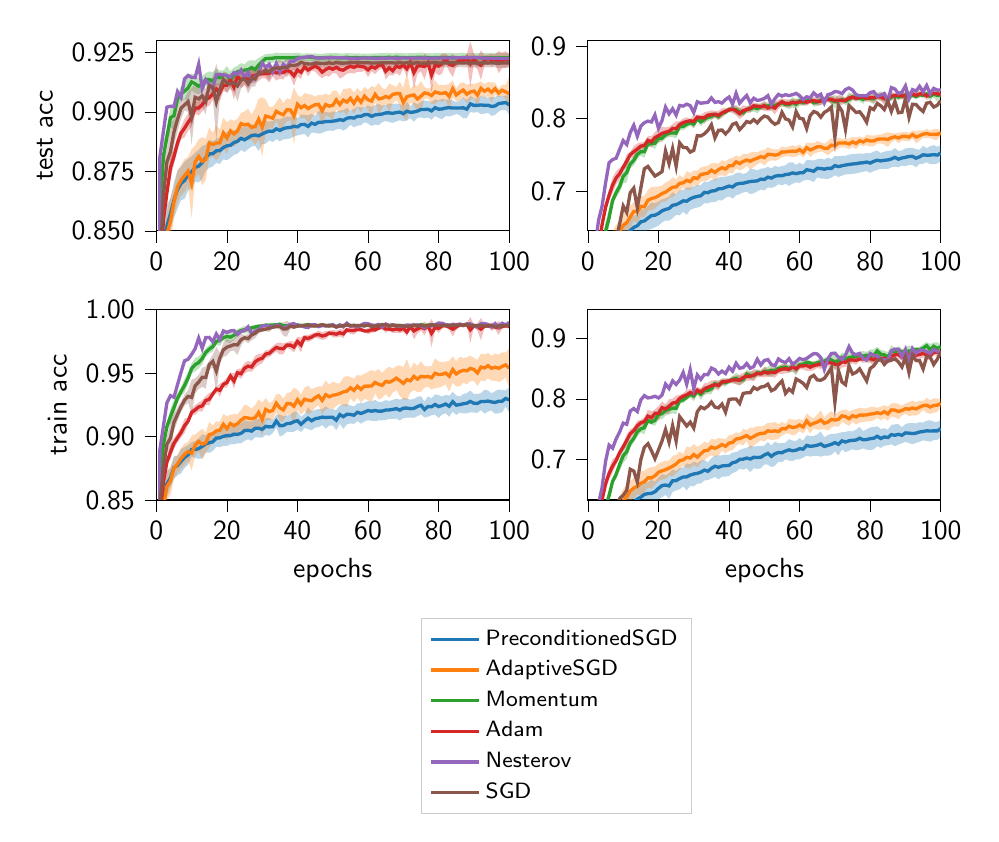
\begin{tikzpicture}

every axis plot post./append style={line width = 1pt}
\definecolor{color0}{rgb}{0.12156862745098,0.466666666666667,0.705882352941177}
\definecolor{color1}{rgb}{1,0.498039215686275,0.0549019607843137}
\definecolor{color2}{rgb}{0.172549019607843,0.627450980392157,0.172549019607843}
\definecolor{color3}{rgb}{0.83921568627451,0.152941176470588,0.156862745098039}
\definecolor{color4}{rgb}{0.580392156862745,0.403921568627451,0.741176470588235}
\definecolor{color5}{rgb}{0.549019607843137,0.337254901960784,0.294117647058824}

\begin{groupplot}[group style={group size=2 by 4}]
\nextgroupplot[
height=4cm,
legend style={font=\footnotesize, at={(0 ,0)},xshift=-0.4cm, yshift=-1.5cm,anchor=north,nodes=right},
tick align=outside,
tick pos=left,
tick pos=left,
width=\figurewidth,
x grid style={white!69.01960784313725!black},
xmin=0, xmax=100,
xtick style={color=black},
y grid style={white!69.01960784313725!black},
ylabel={test acc},
ymin=0.85, ymax=0.93,
ytick style={color=black},
ytick={0.85,0.875,0.9,0.925,0.95},
yticklabels={0.850,0.875,0.900,0.925,0.950}
]
\path [fill=color0, fill opacity=0.3]
(axis cs:0,0.111007682638274)
--(axis cs:0,0.0924979263360852)
--(axis cs:1,0.76297921552286)
--(axis cs:2,0.83155016916493)
--(axis cs:3,0.843056777866148)
--(axis cs:4,0.850499124535519)
--(axis cs:5,0.855450064310349)
--(axis cs:6,0.859325402510863)
--(axis cs:7,0.862907970864437)
--(axis cs:8,0.863354276591052)
--(axis cs:9,0.866867979832462)
--(axis cs:10,0.868241971491237)
--(axis cs:11,0.870528612711843)
--(axis cs:12,0.870346242669089)
--(axis cs:13,0.871656481798211)
--(axis cs:14,0.875238175645734)
--(axis cs:15,0.876443738726973)
--(axis cs:16,0.877029479704536)
--(axis cs:17,0.878585937905475)
--(axis cs:18,0.878076505817822)
--(axis cs:19,0.880037401992253)
--(axis cs:20,0.879642603643186)
--(axis cs:21,0.880605762643072)
--(axis cs:22,0.881884546460922)
--(axis cs:23,0.882390090330088)
--(axis cs:24,0.883965951102325)
--(axis cs:25,0.883127623937711)
--(axis cs:26,0.884301873524402)
--(axis cs:27,0.885412154008664)
--(axis cs:28,0.885767417181058)
--(axis cs:29,0.883479946091963)
--(axis cs:30,0.886520018871308)
--(axis cs:31,0.886578317412144)
--(axis cs:32,0.888012146981869)
--(axis cs:33,0.887293353326084)
--(axis cs:34,0.888522100502241)
--(axis cs:35,0.887592093413284)
--(axis cs:36,0.888357215885626)
--(axis cs:37,0.888561783420825)
--(axis cs:38,0.888846762410855)
--(axis cs:39,0.889623863322753)
--(axis cs:40,0.890075471984398)
--(axis cs:41,0.890439360320662)
--(axis cs:42,0.890692178380628)
--(axis cs:43,0.889201905916963)
--(axis cs:44,0.891297688306183)
--(axis cs:45,0.891149909012924)
--(axis cs:46,0.890797541738312)
--(axis cs:47,0.891099081980649)
--(axis cs:48,0.891765611564957)
--(axis cs:49,0.892142951395093)
--(axis cs:50,0.891980277740173)
--(axis cs:51,0.892545177965319)
--(axis cs:52,0.892907596892968)
--(axis cs:53,0.892069818238496)
--(axis cs:54,0.89294140203078)
--(axis cs:55,0.89453125)
--(axis cs:56,0.893509927585066)
--(axis cs:57,0.894151146917784)
--(axis cs:58,0.89433828886688)
--(axis cs:59,0.895617787043878)
--(axis cs:60,0.895044321581043)
--(axis cs:61,0.894059983506438)
--(axis cs:62,0.894636001470808)
--(axis cs:63,0.894386859836862)
--(axis cs:64,0.89555637765601)
--(axis cs:65,0.896171726197189)
--(axis cs:66,0.895657229073162)
--(axis cs:67,0.895353467906326)
--(axis cs:68,0.895932527020615)
--(axis cs:69,0.896432947951868)
--(axis cs:70,0.895957596233472)
--(axis cs:71,0.896343778268077)
--(axis cs:72,0.897327638555985)
--(axis cs:73,0.895817016220665)
--(axis cs:74,0.897469837395564)
--(axis cs:75,0.897636397882161)
--(axis cs:76,0.897264803884074)
--(axis cs:77,0.897598180802494)
--(axis cs:78,0.896652224991367)
--(axis cs:79,0.898238787012784)
--(axis cs:80,0.897442214361603)
--(axis cs:81,0.896886821618047)
--(axis cs:82,0.898225837195667)
--(axis cs:83,0.89806428735852)
--(axis cs:84,0.89845913759604)
--(axis cs:85,0.899036236735507)
--(axis cs:86,0.898568023423398)
--(axis cs:87,0.897251522690764)
--(axis cs:88,0.897347285222789)
--(axis cs:89,0.899955480666042)
--(axis cs:90,0.899611257674555)
--(axis cs:91,0.899916284124532)
--(axis cs:92,0.898973219155661)
--(axis cs:93,0.899226031513666)
--(axis cs:94,0.899550293089722)
--(axis cs:95,0.898311712997274)
--(axis cs:96,0.898611273129953)
--(axis cs:97,0.900051784466905)
--(axis cs:98,0.900774970867429)
--(axis cs:99,0.900867615405095)
--(axis cs:100,0.898842296113972)
--(axis cs:100,0.907047126962951)
--(axis cs:100,0.907047126962951)
--(axis cs:99,0.906844724338494)
--(axis cs:98,0.906596824004366)
--(axis cs:97,0.906819209122839)
--(axis cs:96,0.906316611485432)
--(axis cs:95,0.906135402387341)
--(axis cs:94,0.905978553064124)
--(axis cs:93,0.906162590281206)
--(axis cs:92,0.906775979562288)
--(axis cs:91,0.905512401772904)
--(axis cs:90,0.905737300017752)
--(axis cs:89,0.906715192410881)
--(axis cs:88,0.904876272469519)
--(axis cs:87,0.906093829873339)
--(axis cs:86,0.904617072730447)
--(axis cs:85,0.904088763264493)
--(axis cs:84,0.904705926506524)
--(axis cs:83,0.905381225461993)
--(axis cs:82,0.904959258958179)
--(axis cs:81,0.905496992484517)
--(axis cs:80,0.90474127922814)
--(axis cs:79,0.90522675785901)
--(axis cs:78,0.904108992957351)
--(axis cs:77,0.904525216633403)
--(axis cs:76,0.904718369192849)
--(axis cs:75,0.90432674314348)
--(axis cs:74,0.903111092091616)
--(axis cs:73,0.904022727369078)
--(axis cs:72,0.902191592213246)
--(axis cs:71,0.904157023013974)
--(axis cs:70,0.902459871715246)
--(axis cs:69,0.903286603330183)
--(axis cs:68,0.903406415287078)
--(axis cs:67,0.903344448760341)
--(axis cs:66,0.903421296567864)
--(axis cs:65,0.902886767392555)
--(axis cs:64,0.902560609523478)
--(axis cs:63,0.903349518368266)
--(axis cs:62,0.902759831862526)
--(axis cs:61,0.902073830596126)
--(axis cs:60,0.902651992521521)
--(axis cs:59,0.901958334750994)
--(axis cs:58,0.90185562138953)
--(axis cs:57,0.90208282744119)
--(axis cs:56,0.901221642927755)
--(axis cs:55,0.900540865384615)
--(axis cs:54,0.901669976174348)
--(axis cs:53,0.900698611248683)
--(axis cs:52,0.900501858235237)
--(axis cs:51,0.90002293100904)
--(axis cs:50,0.900127094054699)
--(axis cs:49,0.899663939630548)
--(axis cs:48,0.900021247409402)
--(axis cs:47,0.900106847506531)
--(axis cs:46,0.900388355697585)
--(axis cs:45,0.898333264064)
--(axis cs:44,0.899187087334842)
--(axis cs:43,0.89851844664714)
--(axis cs:42,0.898730898542449)
--(axis cs:41,0.89884349224344)
--(axis cs:40,0.897264271605345)
--(axis cs:39,0.898236713600324)
--(axis cs:38,0.897972147845556)
--(axis cs:37,0.898036774271482)
--(axis cs:36,0.897520187960528)
--(axis cs:35,0.896802938637999)
--(axis cs:34,0.897134950779811)
--(axis cs:33,0.896180204366224)
--(axis cs:32,0.895781923530951)
--(axis cs:31,0.896214150536574)
--(axis cs:30,0.894850173436385)
--(axis cs:29,0.896287682113166)
--(axis cs:28,0.894761428972789)
--(axis cs:27,0.894575826760566)
--(axis cs:26,0.893923286732008)
--(axis cs:25,0.893334715805878)
--(axis cs:24,0.893758407872034)
--(axis cs:23,0.89279019813145)
--(axis cs:22,0.892234043282668)
--(axis cs:21,0.891229173254364)
--(axis cs:20,0.891771659177327)
--(axis cs:19,0.889934553135952)
--(axis cs:18,0.889271250592434)
--(axis cs:17,0.888581530043243)
--(axis cs:16,0.887694077987771)
--(axis cs:15,0.888219722811489)
--(axis cs:14,0.886140029482471)
--(axis cs:13,0.885655216919738)
--(axis cs:12,0.884000712459116)
--(axis cs:11,0.882836771903542)
--(axis cs:10,0.881297291329276)
--(axis cs:9,0.880207340680358)
--(axis cs:8,0.879013511870486)
--(axis cs:7,0.876915747084281)
--(axis cs:6,0.875330046207086)
--(axis cs:5,0.870351217740933)
--(axis cs:4,0.863663535720891)
--(axis cs:3,0.86092960033898)
--(axis cs:2,0.849579638527378)
--(axis cs:1,0.815927034477141)
--(axis cs:0,0.111007682638274)
--cycle;

\path [fill=color1, fill opacity=0.3]
(axis cs:0,0.111007682638274)
--(axis cs:0,0.0924979263360852)
--(axis cs:1,0.767357931325164)
--(axis cs:2,0.823988251690018)
--(axis cs:3,0.839476076127783)
--(axis cs:4,0.844141685990863)
--(axis cs:5,0.855619184496556)
--(axis cs:6,0.861850582952975)
--(axis cs:7,0.864799036163039)
--(axis cs:8,0.866275831188174)
--(axis cs:9,0.869030282341081)
--(axis cs:10,0.855305398184944)
--(axis cs:11,0.872127058011338)
--(axis cs:12,0.874032242573623)
--(axis cs:13,0.869120229550762)
--(axis cs:14,0.871356735262235)
--(axis cs:15,0.88030594789794)
--(axis cs:16,0.881349835203396)
--(axis cs:17,0.879471491704636)
--(axis cs:18,0.881396150957326)
--(axis cs:19,0.884754508407123)
--(axis cs:20,0.882254298001028)
--(axis cs:21,0.88716368735053)
--(axis cs:22,0.885293740044271)
--(axis cs:23,0.886769656759663)
--(axis cs:24,0.890561194084455)
--(axis cs:25,0.888765524153593)
--(axis cs:26,0.888297882439095)
--(axis cs:27,0.8881379504423)
--(axis cs:28,0.88610753116823)
--(axis cs:29,0.888318034628538)
--(axis cs:30,0.881003728751212)
--(axis cs:31,0.891291226382236)
--(axis cs:32,0.893547122975349)
--(axis cs:33,0.892557021440285)
--(axis cs:34,0.896399453228702)
--(axis cs:35,0.892609693538263)
--(axis cs:36,0.893950570919983)
--(axis cs:37,0.896091856589613)
--(axis cs:38,0.89639592717554)
--(axis cs:39,0.886173608308253)
--(axis cs:40,0.899272122871787)
--(axis cs:41,0.897251531927233)
--(axis cs:42,0.89744122660894)
--(axis cs:43,0.89519897780834)
--(axis cs:44,0.897277017155497)
--(axis cs:45,0.899535729585548)
--(axis cs:46,0.899025128748578)
--(axis cs:47,0.89388498871316)
--(axis cs:48,0.898487722590305)
--(axis cs:49,0.897896724245146)
--(axis cs:50,0.89659912517282)
--(axis cs:51,0.901039542623897)
--(axis cs:52,0.899423487973535)
--(axis cs:53,0.900218644384165)
--(axis cs:54,0.898545548511699)
--(axis cs:55,0.901352059609979)
--(axis cs:56,0.899142557600178)
--(axis cs:57,0.901981407419072)
--(axis cs:58,0.899654347412049)
--(axis cs:59,0.902729617721601)
--(axis cs:60,0.900752960910031)
--(axis cs:61,0.898166726041864)
--(axis cs:62,0.90444132796919)
--(axis cs:63,0.898674904315192)
--(axis cs:64,0.901408723942109)
--(axis cs:65,0.903432232478603)
--(axis cs:66,0.899916837409388)
--(axis cs:67,0.903484266149483)
--(axis cs:68,0.904838907369623)
--(axis cs:69,0.902645354938615)
--(axis cs:70,0.89791726665817)
--(axis cs:71,0.896227458095945)
--(axis cs:72,0.904011859118642)
--(axis cs:73,0.902805050178172)
--(axis cs:74,0.899856297686672)
--(axis cs:75,0.900229061253041)
--(axis cs:76,0.90546875)
--(axis cs:77,0.905567938055781)
--(axis cs:78,0.903230199788331)
--(axis cs:79,0.903300042811385)
--(axis cs:80,0.904551656772534)
--(axis cs:81,0.904190638850509)
--(axis cs:82,0.904946821859472)
--(axis cs:83,0.901072226739484)
--(axis cs:84,0.906281140113241)
--(axis cs:85,0.904364836444028)
--(axis cs:86,0.904474727563379)
--(axis cs:87,0.905917527635084)
--(axis cs:88,0.90343719198357)
--(axis cs:89,0.904994885157292)
--(axis cs:90,0.905720775755013)
--(axis cs:91,0.901809488541394)
--(axis cs:92,0.906970532228319)
--(axis cs:93,0.905766538051839)
--(axis cs:94,0.906556692469204)
--(axis cs:95,0.904115429131295)
--(axis cs:96,0.907212492549065)
--(axis cs:97,0.906021455883233)
--(axis cs:98,0.906773558615586)
--(axis cs:99,0.905380029790366)
--(axis cs:100,0.900570101206899)
--(axis cs:100,0.914774450075152)
--(axis cs:100,0.914774450075152)
--(axis cs:99,0.911366765081429)
--(axis cs:98,0.911335415743388)
--(axis cs:97,0.909703704373177)
--(axis cs:96,0.912258661297089)
--(axis cs:95,0.912350917022552)
--(axis cs:94,0.912493788300027)
--(axis cs:93,0.911581218358418)
--(axis cs:92,0.912781070335783)
--(axis cs:91,0.912132819150913)
--(axis cs:90,0.911707108860372)
--(axis cs:89,0.911671781509375)
--(axis cs:88,0.91130639776002)
--(axis cs:87,0.912371735185429)
--(axis cs:86,0.911931522436621)
--(axis cs:85,0.909777791761101)
--(axis cs:84,0.913169981681631)
--(axis cs:83,0.911848446337439)
--(axis cs:82,0.911178979422579)
--(axis cs:81,0.911214008585388)
--(axis cs:80,0.911233599637723)
--(axis cs:79,0.913326559752718)
--(axis cs:78,0.910391595083464)
--(axis cs:77,0.909696485021143)
--(axis cs:76,0.910416666666667)
--(axis cs:75,0.912891932336702)
--(axis cs:74,0.910820785646661)
--(axis cs:73,0.911357610078238)
--(axis cs:72,0.909529807548025)
--(axis cs:71,0.916432798314311)
--(axis cs:70,0.909955329495676)
--(axis cs:69,0.91263910018959)
--(axis cs:68,0.9104255157073)
--(axis cs:67,0.911139131286415)
--(axis cs:66,0.911821944641894)
--(axis cs:65,0.909428344444474)
--(axis cs:64,0.910009545288661)
--(axis cs:63,0.912142403377116)
--(axis cs:62,0.91020210151799)
--(axis cs:61,0.910807632932495)
--(axis cs:60,0.909363224987405)
--(axis cs:59,0.910431439970706)
--(axis cs:58,0.908458633357182)
--(axis cs:57,0.909937663093749)
--(axis cs:56,0.908008884707515)
--(axis cs:55,0.910046177569509)
--(axis cs:54,0.909627528411378)
--(axis cs:53,0.909617092795322)
--(axis cs:52,0.90668628766749)
--(axis cs:51,0.908976483017129)
--(axis cs:50,0.908789496622051)
--(axis cs:49,0.9068508719087)
--(axis cs:48,0.907642085102002)
--(axis cs:47,0.906996421543251)
--(axis cs:46,0.907164775097576)
--(axis cs:45,0.906353693491375)
--(axis cs:44,0.9071901302804)
--(axis cs:43,0.907525381166019)
--(axis cs:42,0.907827202878239)
--(axis cs:41,0.906113852688151)
--(axis cs:40,0.907037973282059)
--(axis cs:39,0.910200590409696)
--(axis cs:38,0.905146540773178)
--(axis cs:37,0.905630899820644)
--(axis cs:36,0.903565454721043)
--(axis cs:35,0.906068191077121)
--(axis cs:34,0.904001187796939)
--(axis cs:33,0.902014292662279)
--(axis cs:32,0.902025793691318)
--(axis cs:31,0.905183132592123)
--(axis cs:30,0.906095630223147)
--(axis cs:29,0.905451997422744)
--(axis cs:28,0.90149262908818)
--(axis cs:27,0.898841216224366)
--(axis cs:26,0.901285450894239)
--(axis cs:25,0.900096655333586)
--(axis cs:24,0.899542972582211)
--(axis cs:23,0.897084509907003)
--(axis cs:22,0.896156580468549)
--(axis cs:21,0.896830703675111)
--(axis cs:20,0.895650349434869)
--(axis cs:19,0.897517126208262)
--(axis cs:18,0.892562182376008)
--(axis cs:17,0.894246457013313)
--(axis cs:16,0.891226286591475)
--(axis cs:15,0.893391968768726)
--(axis cs:14,0.888539098071099)
--(axis cs:13,0.889273199936417)
--(axis cs:12,0.888427693323812)
--(axis cs:11,0.885865730450201)
--(axis cs:10,0.884217838994543)
--(axis cs:9,0.881089909966612)
--(axis cs:8,0.880098367529775)
--(axis cs:7,0.877749040760038)
--(axis cs:6,0.875248776021384)
--(axis cs:5,0.868539469349598)
--(axis cs:4,0.864091487086059)
--(axis cs:3,0.857859661051704)
--(axis cs:2,0.849509344463828)
--(axis cs:1,0.817237421238939)
--(axis cs:0,0.111007682638274)
--cycle;

\path [fill=color2, fill opacity=0.3]
(axis cs:0,0.111007682638274)
--(axis cs:0,0.0924979263360852)
--(axis cs:1,0.850799855329213)
--(axis cs:2,0.87560370681279)
--(axis cs:3,0.885499983070401)
--(axis cs:4,0.89339108460755)
--(axis cs:5,0.892498462084589)
--(axis cs:6,0.902856502055989)
--(axis cs:7,0.90463964463763)
--(axis cs:8,0.905352978584738)
--(axis cs:9,0.904438500694745)
--(axis cs:10,0.909102340626144)
--(axis cs:11,0.907873620945282)
--(axis cs:12,0.907336771777903)
--(axis cs:13,0.908187249486688)
--(axis cs:14,0.910886665092065)
--(axis cs:15,0.910100256430374)
--(axis cs:16,0.908913488462689)
--(axis cs:17,0.911127081023934)
--(axis cs:18,0.911262467624969)
--(axis cs:19,0.913432477056829)
--(axis cs:20,0.91116093559555)
--(axis cs:21,0.910059959758254)
--(axis cs:22,0.912367068643893)
--(axis cs:23,0.91433390280934)
--(axis cs:24,0.913819020970641)
--(axis cs:25,0.915050838589793)
--(axis cs:26,0.91397647515203)
--(axis cs:27,0.91549991775685)
--(axis cs:28,0.913970669096518)
--(axis cs:29,0.916710726336719)
--(axis cs:30,0.918808801338863)
--(axis cs:31,0.920537623084801)
--(axis cs:32,0.920440660657953)
--(axis cs:33,0.920606593760343)
--(axis cs:34,0.920671169973107)
--(axis cs:35,0.920705897879316)
--(axis cs:36,0.92086772848169)
--(axis cs:37,0.920801828458728)
--(axis cs:38,0.920811736914329)
--(axis cs:39,0.920817921574742)
--(axis cs:40,0.920856472762651)
--(axis cs:41,0.921156967829275)
--(axis cs:42,0.921197108685935)
--(axis cs:43,0.921162552441444)
--(axis cs:44,0.921131358029598)
--(axis cs:45,0.920956978912637)
--(axis cs:46,0.92091510237542)
--(axis cs:47,0.921006720121478)
--(axis cs:48,0.920994155711085)
--(axis cs:49,0.921045469222389)
--(axis cs:50,0.921075076574486)
--(axis cs:51,0.920865253746635)
--(axis cs:52,0.920754383855065)
--(axis cs:53,0.920986194822124)
--(axis cs:54,0.921123600030981)
--(axis cs:55,0.920840314224777)
--(axis cs:56,0.92089157962823)
--(axis cs:57,0.920959768643848)
--(axis cs:58,0.920895445016319)
--(axis cs:59,0.921063145567569)
--(axis cs:60,0.920772361670494)
--(axis cs:61,0.920970698302989)
--(axis cs:62,0.921030108896088)
--(axis cs:63,0.920924380870966)
--(axis cs:64,0.920968282147695)
--(axis cs:65,0.920890285674869)
--(axis cs:66,0.92112939252192)
--(axis cs:67,0.920925565445076)
--(axis cs:68,0.921099651075773)
--(axis cs:69,0.920917049603853)
--(axis cs:70,0.921061739646564)
--(axis cs:71,0.920827246673203)
--(axis cs:72,0.921016375530192)
--(axis cs:73,0.920861395145628)
--(axis cs:74,0.92104391352087)
--(axis cs:75,0.920889708408367)
--(axis cs:76,0.920908647178788)
--(axis cs:77,0.920918237098153)
--(axis cs:78,0.920827246673203)
--(axis cs:79,0.920986961401899)
--(axis cs:80,0.920873076093656)
--(axis cs:81,0.92087732520953)
--(axis cs:82,0.920924927804612)
--(axis cs:83,0.920767882294274)
--(axis cs:84,0.920969039804023)
--(axis cs:85,0.920805817603985)
--(axis cs:86,0.920681736550385)
--(axis cs:87,0.920881203039163)
--(axis cs:88,0.920860986642224)
--(axis cs:89,0.920748571767299)
--(axis cs:90,0.920897803258808)
--(axis cs:91,0.920781767025592)
--(axis cs:92,0.920724751150585)
--(axis cs:93,0.920668789023482)
--(axis cs:94,0.920712017099597)
--(axis cs:95,0.920715044975319)
--(axis cs:96,0.920661384137565)
--(axis cs:97,0.920623168645676)
--(axis cs:98,0.920596683591954)
--(axis cs:99,0.920651142730012)
--(axis cs:100,0.920716273585015)
--(axis cs:100,0.924556162312421)
--(axis cs:100,0.924556162312421)
--(axis cs:99,0.924661357269988)
--(axis cs:98,0.924675752305483)
--(axis cs:97,0.924709363405606)
--(axis cs:96,0.924791340221409)
--(axis cs:95,0.924717647332373)
--(axis cs:94,0.924640547002967)
--(axis cs:93,0.924603646873954)
--(axis cs:92,0.924687909105825)
--(axis cs:91,0.924630893230818)
--(axis cs:90,0.924655081356577)
--(axis cs:89,0.924563928232701)
--(axis cs:88,0.924591737716751)
--(axis cs:87,0.924831937986478)
--(axis cs:86,0.924750955757307)
--(axis cs:85,0.924566778549861)
--(axis cs:84,0.924704037119054)
--(axis cs:83,0.924744938218546)
--(axis cs:82,0.924728117067183)
--(axis cs:81,0.924755687610982)
--(axis cs:80,0.924619712367882)
--(axis cs:79,0.924626019367332)
--(axis cs:78,0.924525317429361)
--(axis cs:77,0.924694743671078)
--(axis cs:76,0.924664269487879)
--(axis cs:75,0.924883528771121)
--(axis cs:74,0.924749355709899)
--(axis cs:73,0.924651425367193)
--(axis cs:72,0.924656701392885)
--(axis cs:71,0.924525317429361)
--(axis cs:70,0.92459130522523)
--(axis cs:69,0.92471596321666)
--(axis cs:68,0.924833842513971)
--(axis cs:67,0.924527158913899)
--(axis cs:66,0.924764036965259)
--(axis cs:65,0.924722695094362)
--(axis cs:64,0.924624666570254)
--(axis cs:63,0.924588439641855)
--(axis cs:62,0.924542807770579)
--(axis cs:61,0.924482026055985)
--(axis cs:60,0.924439978073096)
--(axis cs:59,0.924489739047815)
--(axis cs:58,0.924477151137527)
--(axis cs:57,0.924553051868973)
--(axis cs:56,0.924581176782026)
--(axis cs:55,0.924512249877787)
--(axis cs:54,0.924669669199788)
--(axis cs:53,0.924466529536851)
--(axis cs:52,0.924498019991089)
--(axis cs:51,0.924667598817467)
--(axis cs:50,0.924618032399873)
--(axis cs:49,0.924667671803253)
--(axis cs:48,0.924538696853017)
--(axis cs:47,0.924385908083651)
--(axis cs:46,0.924337301470734)
--(axis cs:45,0.924555841600184)
--(axis cs:44,0.924401494534505)
--(axis cs:43,0.924610684738044)
--(axis cs:42,0.92445593618586)
--(axis cs:41,0.92449607704252)
--(axis cs:40,0.92485666826299)
--(axis cs:39,0.924634802784233)
--(axis cs:38,0.924661019495928)
--(axis cs:37,0.9245907997464)
--(axis cs:36,0.924625059979849)
--(axis cs:35,0.924646666223248)
--(axis cs:34,0.924881714642277)
--(axis cs:33,0.92444548957299)
--(axis cs:32,0.924411102162559)
--(axis cs:31,0.924234011530584)
--(axis cs:30,0.923458826866265)
--(axis cs:29,0.92263222238123)
--(axis cs:28,0.921526125775276)
--(axis cs:27,0.921659537371356)
--(axis cs:26,0.921400127412073)
--(axis cs:25,0.919965187051233)
--(axis cs:24,0.920435786721667)
--(axis cs:23,0.919400071549634)
--(axis cs:22,0.91852235443303)
--(axis cs:21,0.917003341523798)
--(axis cs:20,0.919227686199322)
--(axis cs:19,0.917396849866248)
--(axis cs:18,0.917383365708364)
--(axis cs:17,0.91819984205299)
--(axis cs:16,0.916687473075773)
--(axis cs:15,0.916943012800396)
--(axis cs:14,0.916336892600243)
--(axis cs:13,0.915110026154337)
--(axis cs:12,0.914177651299021)
--(axis cs:11,0.915704103413692)
--(axis cs:10,0.915997819630266)
--(axis cs:9,0.91553345443346)
--(axis cs:8,0.911974745774236)
--(axis cs:7,0.910724938695703)
--(axis cs:6,0.90778051717478)
--(axis cs:5,0.904356505864129)
--(axis cs:4,0.901600902571937)
--(axis cs:3,0.893426298980881)
--(axis cs:2,0.886856229084646)
--(axis cs:1,0.8651456574913)
--(axis cs:0,0.111007682638274)
--cycle;

\path [fill=color3, fill opacity=0.3]
(axis cs:0,0.111007682638274)
--(axis cs:0,0.0924979263360852)
--(axis cs:1,0.823085043334398)
--(axis cs:2,0.849963351775444)
--(axis cs:3,0.862794914188911)
--(axis cs:4,0.871848324791142)
--(axis cs:5,0.878048349291724)
--(axis cs:6,0.883947039135817)
--(axis cs:7,0.888395735926279)
--(axis cs:8,0.889250819955163)
--(axis cs:9,0.891946560522721)
--(axis cs:10,0.893702639801253)
--(axis cs:11,0.899273557489459)
--(axis cs:12,0.898353698249277)
--(axis cs:13,0.900199594809115)
--(axis cs:14,0.901954711002708)
--(axis cs:15,0.902521152712122)
--(axis cs:16,0.904924020302207)
--(axis cs:17,0.907243638139041)
--(axis cs:18,0.904421885366375)
--(axis cs:19,0.908655324375179)
--(axis cs:20,0.908279529915436)
--(axis cs:21,0.910463074271104)
--(axis cs:22,0.904982844883875)
--(axis cs:23,0.912385254591265)
--(axis cs:24,0.909932343316078)
--(axis cs:25,0.911332053827296)
--(axis cs:26,0.909682297465792)
--(axis cs:27,0.911876716018362)
--(axis cs:28,0.912204659882383)
--(axis cs:29,0.912985127459992)
--(axis cs:30,0.914210907766019)
--(axis cs:31,0.913914936762794)
--(axis cs:32,0.912327574332861)
--(axis cs:33,0.91490900357571)
--(axis cs:34,0.913138600310717)
--(axis cs:35,0.913889264873332)
--(axis cs:36,0.913556271281996)
--(axis cs:37,0.915845750604255)
--(axis cs:38,0.914808969430715)
--(axis cs:39,0.910854856669442)
--(axis cs:40,0.914891703512845)
--(axis cs:41,0.913772837365643)
--(axis cs:42,0.917515508397026)
--(axis cs:43,0.914828470462772)
--(axis cs:44,0.917159977809341)
--(axis cs:45,0.916943901594713)
--(axis cs:46,0.91519603336275)
--(axis cs:47,0.914207014834707)
--(axis cs:48,0.915142396413288)
--(axis cs:49,0.914717292910301)
--(axis cs:50,0.916211853114733)
--(axis cs:51,0.916143948659156)
--(axis cs:52,0.913937381510636)
--(axis cs:53,0.914767912488614)
--(axis cs:54,0.915927759941007)
--(axis cs:55,0.916340415779966)
--(axis cs:56,0.916083010523234)
--(axis cs:57,0.916804408282112)
--(axis cs:58,0.916746621440621)
--(axis cs:59,0.917249046532634)
--(axis cs:60,0.914559469183371)
--(axis cs:61,0.917036866356369)
--(axis cs:62,0.91580241697853)
--(axis cs:63,0.91749433269562)
--(axis cs:64,0.918387490234008)
--(axis cs:65,0.913556988551496)
--(axis cs:66,0.91544044106881)
--(axis cs:67,0.915256001150585)
--(axis cs:68,0.916352886381834)
--(axis cs:69,0.915157591909195)
--(axis cs:70,0.918143670384063)
--(axis cs:71,0.91476628145947)
--(axis cs:72,0.918643342565959)
--(axis cs:73,0.909780598319845)
--(axis cs:74,0.915948945184382)
--(axis cs:75,0.916979163297106)
--(axis cs:76,0.913527507967507)
--(axis cs:77,0.918356518246661)
--(axis cs:78,0.90814911106571)
--(axis cs:79,0.916619862882028)
--(axis cs:80,0.915266058687097)
--(axis cs:81,0.916035499797822)
--(axis cs:82,0.920153734863406)
--(axis cs:83,0.916992983771072)
--(axis cs:84,0.914587183996481)
--(axis cs:85,0.918877863918772)
--(axis cs:86,0.920190835542859)
--(axis cs:87,0.919668705036431)
--(axis cs:88,0.921098703747338)
--(axis cs:89,0.910576206167358)
--(axis cs:90,0.91987472179813)
--(axis cs:91,0.91783852240515)
--(axis cs:92,0.913389603244871)
--(axis cs:93,0.919204185820254)
--(axis cs:94,0.921148253700862)
--(axis cs:95,0.918932440908827)
--(axis cs:96,0.920235959860263)
--(axis cs:97,0.91620545665155)
--(axis cs:98,0.918289940899026)
--(axis cs:99,0.918607447119559)
--(axis cs:100,0.919155831065073)
--(axis cs:100,0.924253624063132)
--(axis cs:100,0.924253624063132)
--(axis cs:99,0.925503129803517)
--(axis cs:98,0.924799001408666)
--(axis cs:97,0.925541338220245)
--(axis cs:96,0.924034873473071)
--(axis cs:95,0.924336789860403)
--(axis cs:94,0.924024021940164)
--(axis cs:93,0.92380462828231)
--(axis cs:92,0.925773057011539)
--(axis cs:91,0.923046894261517)
--(axis cs:90,0.924396111535203)
--(axis cs:89,0.929608088704437)
--(axis cs:88,0.924333988560354)
--(axis cs:87,0.922859339835364)
--(axis cs:86,0.922918138816115)
--(axis cs:85,0.922688642491485)
--(axis cs:84,0.924274995490699)
--(axis cs:83,0.923071118793031)
--(axis cs:82,0.924457643341722)
--(axis cs:81,0.92432908353551)
--(axis cs:80,0.923115351569314)
--(axis cs:79,0.922342476861562)
--(axis cs:78,0.922740312011213)
--(axis cs:77,0.922889475343083)
--(axis cs:76,0.924453261263263)
--(axis cs:75,0.921742791831099)
--(axis cs:74,0.922492561225874)
--(axis cs:73,0.923132061936566)
--(axis cs:72,0.922602651023784)
--(axis cs:71,0.921251346745657)
--(axis cs:70,0.921139182180039)
--(axis cs:69,0.922081991424138)
--(axis cs:68,0.922008491823294)
--(axis cs:67,0.919219159105825)
--(axis cs:66,0.921458597392728)
--(axis cs:65,0.920377306320299)
--(axis cs:64,0.921296003355736)
--(axis cs:63,0.92146800704797)
--(axis cs:62,0.920836204816342)
--(axis cs:61,0.920863774669272)
--(axis cs:60,0.920636844919193)
--(axis cs:59,0.92029101756993)
--(axis cs:58,0.921374372149122)
--(axis cs:57,0.921817386589682)
--(axis cs:56,0.921236701015227)
--(axis cs:55,0.921940834220034)
--(axis cs:54,0.921031374674378)
--(axis cs:53,0.920188016998565)
--(axis cs:52,0.921599477463723)
--(axis cs:51,0.921255891084433)
--(axis cs:50,0.919525326372447)
--(axis cs:49,0.922281905807647)
--(axis cs:48,0.92039446256107)
--(axis cs:47,0.91906622234478)
--(axis cs:46,0.921542748688533)
--(axis cs:45,0.921317316354006)
--(axis cs:44,0.919739060652198)
--(axis cs:43,0.920227619280818)
--(axis cs:42,0.920184812115794)
--(axis cs:41,0.919400239557434)
--(axis cs:40,0.920224482384591)
--(axis cs:39,0.919313412561327)
--(axis cs:38,0.918904972876977)
--(axis cs:37,0.91886979426754)
--(axis cs:36,0.919476581282107)
--(axis cs:35,0.919343908203591)
--(axis cs:34,0.919593771484154)
--(axis cs:33,0.919105419501214)
--(axis cs:32,0.919924028231241)
--(axis cs:31,0.918296601698745)
--(axis cs:30,0.917880438387827)
--(axis cs:29,0.918505257155393)
--(axis cs:28,0.918444378579156)
--(axis cs:27,0.918011104494459)
--(axis cs:26,0.91768148458549)
--(axis cs:25,0.917073394890653)
--(axis cs:24,0.91671028488905)
--(axis cs:23,0.917242149254889)
--(axis cs:22,0.91577036024433)
--(axis cs:21,0.91633981034428)
--(axis cs:20,0.914076239315333)
--(axis cs:19,0.913540188445334)
--(axis cs:18,0.911683883864394)
--(axis cs:17,0.911886970835318)
--(axis cs:16,0.910120050210613)
--(axis cs:15,0.909337821646852)
--(axis cs:14,0.908341763356266)
--(axis cs:13,0.905729892370372)
--(axis cs:12,0.904911526109698)
--(axis cs:11,0.903831410459259)
--(axis cs:10,0.901629892250029)
--(axis cs:9,0.89917924075933)
--(axis cs:8,0.896987160814067)
--(axis cs:7,0.893675578176285)
--(axis cs:6,0.889790941633414)
--(axis cs:5,0.884391554554429)
--(axis cs:4,0.880976194439627)
--(axis cs:3,0.869216303759807)
--(axis cs:2,0.85877062258353)
--(axis cs:1,0.834887713075858)
--(axis cs:0,0.111007682638274)
--cycle;

\path [fill=color4, fill opacity=0.3]
(axis cs:0,0.098056891025641)
--(axis cs:0,0.098056891025641)
--(axis cs:1,0.881109775641026)
--(axis cs:2,0.891726762820513)
--(axis cs:3,0.901943108974359)
--(axis cs:4,0.90234375)
--(axis cs:5,0.90214342948718)
--(axis cs:6,0.908453525641026)
--(axis cs:7,0.90614983974359)
--(axis cs:8,0.91386217948718)
--(axis cs:9,0.915264423076923)
--(axis cs:10,0.914463141025641)
--(axis cs:11,0.914362980769231)
--(axis cs:12,0.919971955128205)
--(axis cs:13,0.909755608974359)
--(axis cs:14,0.913461538461538)
--(axis cs:15,0.911558493589744)
--(axis cs:16,0.909855769230769)
--(axis cs:17,0.915665064102564)
--(axis cs:18,0.915765224358974)
--(axis cs:19,0.915464743589744)
--(axis cs:20,0.915264423076923)
--(axis cs:21,0.914563301282051)
--(axis cs:22,0.916466346153846)
--(axis cs:23,0.915765224358974)
--(axis cs:24,0.917568108974359)
--(axis cs:25,0.914463141025641)
--(axis cs:26,0.916566506410256)
--(axis cs:27,0.913261217948718)
--(axis cs:28,0.914663461538462)
--(axis cs:29,0.916065705128205)
--(axis cs:30,0.920472756410256)
--(axis cs:31,0.918669871794872)
--(axis cs:32,0.919971955128205)
--(axis cs:33,0.916766826923077)
--(axis cs:34,0.920272435897436)
--(axis cs:35,0.916766826923077)
--(axis cs:36,0.919971955128205)
--(axis cs:37,0.918569711538462)
--(axis cs:38,0.921274038461538)
--(axis cs:39,0.921274038461538)
--(axis cs:40,0.922375801282051)
--(axis cs:41,0.922776442307692)
--(axis cs:42,0.922876602564103)
--(axis cs:43,0.923076923076923)
--(axis cs:44,0.923277243589744)
--(axis cs:45,0.922676282051282)
--(axis cs:46,0.922576121794872)
--(axis cs:47,0.922576121794872)
--(axis cs:48,0.922776442307692)
--(axis cs:49,0.922676282051282)
--(axis cs:50,0.922676282051282)
--(axis cs:51,0.922676282051282)
--(axis cs:52,0.922676282051282)
--(axis cs:53,0.922676282051282)
--(axis cs:54,0.922576121794872)
--(axis cs:55,0.922475961538462)
--(axis cs:56,0.922475961538462)
--(axis cs:57,0.922375801282051)
--(axis cs:58,0.922576121794872)
--(axis cs:59,0.922576121794872)
--(axis cs:60,0.922576121794872)
--(axis cs:61,0.922576121794872)
--(axis cs:62,0.922375801282051)
--(axis cs:63,0.922475961538462)
--(axis cs:64,0.922576121794872)
--(axis cs:65,0.922475961538462)
--(axis cs:66,0.922576121794872)
--(axis cs:67,0.922576121794872)
--(axis cs:68,0.922475961538462)
--(axis cs:69,0.922576121794872)
--(axis cs:70,0.922576121794872)
--(axis cs:71,0.922576121794872)
--(axis cs:72,0.922576121794872)
--(axis cs:73,0.922576121794872)
--(axis cs:74,0.922576121794872)
--(axis cs:75,0.922576121794872)
--(axis cs:76,0.922676282051282)
--(axis cs:77,0.922475961538462)
--(axis cs:78,0.922576121794872)
--(axis cs:79,0.922576121794872)
--(axis cs:80,0.922576121794872)
--(axis cs:81,0.922576121794872)
--(axis cs:82,0.922576121794872)
--(axis cs:83,0.922576121794872)
--(axis cs:84,0.922676282051282)
--(axis cs:85,0.922776442307692)
--(axis cs:86,0.922676282051282)
--(axis cs:87,0.922676282051282)
--(axis cs:88,0.922676282051282)
--(axis cs:89,0.922776442307692)
--(axis cs:90,0.922776442307692)
--(axis cs:91,0.922876602564103)
--(axis cs:92,0.922676282051282)
--(axis cs:93,0.922475961538462)
--(axis cs:94,0.922576121794872)
--(axis cs:95,0.922475961538462)
--(axis cs:96,0.922475961538462)
--(axis cs:97,0.922475961538462)
--(axis cs:98,0.922375801282051)
--(axis cs:99,0.922375801282051)
--(axis cs:100,0.922375801282051)
--(axis cs:100,0.922375801282051)
--(axis cs:100,0.922375801282051)
--(axis cs:99,0.922375801282051)
--(axis cs:98,0.922375801282051)
--(axis cs:97,0.922475961538462)
--(axis cs:96,0.922475961538462)
--(axis cs:95,0.922475961538462)
--(axis cs:94,0.922576121794872)
--(axis cs:93,0.922475961538462)
--(axis cs:92,0.922676282051282)
--(axis cs:91,0.922876602564103)
--(axis cs:90,0.922776442307692)
--(axis cs:89,0.922776442307692)
--(axis cs:88,0.922676282051282)
--(axis cs:87,0.922676282051282)
--(axis cs:86,0.922676282051282)
--(axis cs:85,0.922776442307692)
--(axis cs:84,0.922676282051282)
--(axis cs:83,0.922576121794872)
--(axis cs:82,0.922576121794872)
--(axis cs:81,0.922576121794872)
--(axis cs:80,0.922576121794872)
--(axis cs:79,0.922576121794872)
--(axis cs:78,0.922576121794872)
--(axis cs:77,0.922475961538462)
--(axis cs:76,0.922676282051282)
--(axis cs:75,0.922576121794872)
--(axis cs:74,0.922576121794872)
--(axis cs:73,0.922576121794872)
--(axis cs:72,0.922576121794872)
--(axis cs:71,0.922576121794872)
--(axis cs:70,0.922576121794872)
--(axis cs:69,0.922576121794872)
--(axis cs:68,0.922475961538462)
--(axis cs:67,0.922576121794872)
--(axis cs:66,0.922576121794872)
--(axis cs:65,0.922475961538462)
--(axis cs:64,0.922576121794872)
--(axis cs:63,0.922475961538462)
--(axis cs:62,0.922375801282051)
--(axis cs:61,0.922576121794872)
--(axis cs:60,0.922576121794872)
--(axis cs:59,0.922576121794872)
--(axis cs:58,0.922576121794872)
--(axis cs:57,0.922375801282051)
--(axis cs:56,0.922475961538462)
--(axis cs:55,0.922475961538462)
--(axis cs:54,0.922576121794872)
--(axis cs:53,0.922676282051282)
--(axis cs:52,0.922676282051282)
--(axis cs:51,0.922676282051282)
--(axis cs:50,0.922676282051282)
--(axis cs:49,0.922676282051282)
--(axis cs:48,0.922776442307692)
--(axis cs:47,0.922576121794872)
--(axis cs:46,0.922576121794872)
--(axis cs:45,0.922676282051282)
--(axis cs:44,0.923277243589744)
--(axis cs:43,0.923076923076923)
--(axis cs:42,0.922876602564103)
--(axis cs:41,0.922776442307692)
--(axis cs:40,0.922375801282051)
--(axis cs:39,0.921274038461538)
--(axis cs:38,0.921274038461538)
--(axis cs:37,0.918569711538462)
--(axis cs:36,0.919971955128205)
--(axis cs:35,0.916766826923077)
--(axis cs:34,0.920272435897436)
--(axis cs:33,0.916766826923077)
--(axis cs:32,0.919971955128205)
--(axis cs:31,0.918669871794872)
--(axis cs:30,0.920472756410256)
--(axis cs:29,0.916065705128205)
--(axis cs:28,0.914663461538462)
--(axis cs:27,0.913261217948718)
--(axis cs:26,0.916566506410256)
--(axis cs:25,0.914463141025641)
--(axis cs:24,0.917568108974359)
--(axis cs:23,0.915765224358974)
--(axis cs:22,0.916466346153846)
--(axis cs:21,0.914563301282051)
--(axis cs:20,0.915264423076923)
--(axis cs:19,0.915464743589744)
--(axis cs:18,0.915765224358974)
--(axis cs:17,0.915665064102564)
--(axis cs:16,0.909855769230769)
--(axis cs:15,0.911558493589744)
--(axis cs:14,0.913461538461538)
--(axis cs:13,0.909755608974359)
--(axis cs:12,0.919971955128205)
--(axis cs:11,0.914362980769231)
--(axis cs:10,0.914463141025641)
--(axis cs:9,0.915264423076923)
--(axis cs:8,0.91386217948718)
--(axis cs:7,0.90614983974359)
--(axis cs:6,0.908453525641026)
--(axis cs:5,0.90214342948718)
--(axis cs:4,0.90234375)
--(axis cs:3,0.901943108974359)
--(axis cs:2,0.891726762820513)
--(axis cs:1,0.881109775641026)
--(axis cs:0,0.098056891025641)
--cycle;

\path [fill=color5, fill opacity=0.3]
(axis cs:0,0.111007682638274)
--(axis cs:0,0.0924979263360852)
--(axis cs:1,0.810648874259321)
--(axis cs:2,0.849684745338958)
--(axis cs:3,0.873554516522459)
--(axis cs:4,0.871482732793603)
--(axis cs:5,0.885963584820602)
--(axis cs:6,0.891401640523487)
--(axis cs:7,0.897050463535066)
--(axis cs:8,0.900520412529061)
--(axis cs:9,0.900031386126153)
--(axis cs:10,0.886039692179554)
--(axis cs:11,0.900265926363599)
--(axis cs:12,0.900249364270127)
--(axis cs:13,0.901917850374227)
--(axis cs:14,0.898864915972289)
--(axis cs:15,0.908920532269978)
--(axis cs:16,0.905901904050624)
--(axis cs:17,0.887852632990764)
--(axis cs:18,0.905517613536564)
--(axis cs:19,0.91027771732051)
--(axis cs:20,0.907748721346964)
--(axis cs:21,0.909608315122319)
--(axis cs:22,0.908146505030916)
--(axis cs:23,0.904305204010714)
--(axis cs:24,0.909683709628014)
--(axis cs:25,0.911496914032297)
--(axis cs:26,0.907647250716046)
--(axis cs:27,0.910525627867481)
--(axis cs:28,0.910567392239248)
--(axis cs:29,0.914696054644621)
--(axis cs:30,0.915067197970075)
--(axis cs:31,0.915028889662756)
--(axis cs:32,0.913199414930945)
--(axis cs:33,0.916880416909119)
--(axis cs:34,0.915513857422884)
--(axis cs:35,0.91500310688817)
--(axis cs:36,0.916177181721692)
--(axis cs:37,0.914300783864795)
--(axis cs:38,0.917880074253735)
--(axis cs:39,0.917334691149585)
--(axis cs:40,0.917727879227053)
--(axis cs:41,0.918962870147416)
--(axis cs:42,0.918680656101409)
--(axis cs:43,0.918475023628966)
--(axis cs:44,0.918497336217385)
--(axis cs:45,0.918916226572921)
--(axis cs:46,0.918993392649431)
--(axis cs:47,0.918529298075078)
--(axis cs:48,0.91854911687788)
--(axis cs:49,0.918902943887662)
--(axis cs:50,0.918441914033673)
--(axis cs:51,0.918993802482969)
--(axis cs:52,0.918716702621953)
--(axis cs:53,0.918774019107013)
--(axis cs:54,0.918889980083829)
--(axis cs:55,0.918684400382218)
--(axis cs:56,0.918907365209978)
--(axis cs:57,0.918917469105248)
--(axis cs:58,0.918739430537627)
--(axis cs:59,0.918871140836234)
--(axis cs:60,0.918710471590387)
--(axis cs:61,0.91878155114418)
--(axis cs:62,0.918682215424575)
--(axis cs:63,0.918669534207991)
--(axis cs:64,0.918727277411558)
--(axis cs:65,0.918769692557495)
--(axis cs:66,0.918885969862948)
--(axis cs:67,0.918669552161607)
--(axis cs:68,0.91888871322299)
--(axis cs:69,0.918853350059616)
--(axis cs:70,0.918632546357315)
--(axis cs:71,0.918738359734543)
--(axis cs:72,0.918615522576138)
--(axis cs:73,0.91866719516966)
--(axis cs:74,0.918881071030835)
--(axis cs:75,0.918399670255296)
--(axis cs:76,0.918725385458095)
--(axis cs:77,0.918645814955401)
--(axis cs:78,0.918822589471949)
--(axis cs:79,0.918905170810198)
--(axis cs:80,0.91868856141792)
--(axis cs:81,0.918665781459547)
--(axis cs:82,0.918616681188318)
--(axis cs:83,0.91873570007042)
--(axis cs:84,0.918775411846007)
--(axis cs:85,0.918565265193296)
--(axis cs:86,0.918796560644461)
--(axis cs:87,0.918624938428977)
--(axis cs:88,0.918744797161867)
--(axis cs:89,0.918529011604543)
--(axis cs:90,0.918648324424173)
--(axis cs:91,0.918688157749814)
--(axis cs:92,0.918623425300873)
--(axis cs:93,0.91870176866063)
--(axis cs:94,0.918632576664844)
--(axis cs:95,0.918690520314251)
--(axis cs:96,0.918700688313977)
--(axis cs:97,0.918428981384106)
--(axis cs:98,0.91857200824914)
--(axis cs:99,0.918389423076923)
--(axis cs:100,0.918675836870983)
--(axis cs:100,0.92236983620594)
--(axis cs:100,0.92236983620594)
--(axis cs:99,0.922536057692308)
--(axis cs:98,0.922413568673937)
--(axis cs:97,0.922396339128714)
--(axis cs:96,0.922224792455254)
--(axis cs:95,0.922595537378057)
--(axis cs:94,0.922252840001823)
--(axis cs:93,0.922444064672703)
--(axis cs:92,0.922402215724768)
--(axis cs:91,0.922137162763007)
--(axis cs:90,0.922357284550185)
--(axis cs:89,0.922316340959559)
--(axis cs:88,0.922220747709928)
--(axis cs:87,0.922420734647946)
--(axis cs:86,0.922249112432462)
--(axis cs:85,0.922360215575934)
--(axis cs:84,0.922350389436044)
--(axis cs:83,0.922510293519324)
--(axis cs:82,0.922328831632195)
--(axis cs:81,0.922299763412248)
--(axis cs:80,0.922276983453875)
--(axis cs:79,0.922461015087238)
--(axis cs:78,0.922343275912666)
--(axis cs:77,0.922139441454855)
--(axis cs:76,0.922320287618828)
--(axis cs:75,0.922305457949833)
--(axis cs:74,0.922485114866601)
--(axis cs:73,0.922118061240597)
--(axis cs:72,0.922450182552068)
--(axis cs:71,0.9225076338552)
--(axis cs:70,0.922292934411916)
--(axis cs:69,0.922372611478846)
--(axis cs:68,0.922076831648805)
--(axis cs:67,0.922436217069162)
--(axis cs:66,0.922380055778078)
--(axis cs:65,0.922316044621992)
--(axis cs:64,0.922458620024339)
--(axis cs:63,0.922235914509957)
--(axis cs:62,0.922343425601066)
--(axis cs:61,0.922183993727615)
--(axis cs:60,0.922455393794229)
--(axis cs:59,0.922254660445817)
--(axis cs:58,0.922546627154681)
--(axis cs:57,0.922248396279368)
--(axis cs:56,0.922518916841304)
--(axis cs:55,0.922481465002398)
--(axis cs:54,0.922175725044376)
--(axis cs:53,0.922091365508372)
--(axis cs:52,0.922208778147277)
--(axis cs:51,0.922512607773441)
--(axis cs:50,0.922143021863763)
--(axis cs:49,0.922202825343107)
--(axis cs:48,0.922115947224684)
--(axis cs:47,0.92197550961723)
--(axis cs:46,0.921791863760825)
--(axis cs:45,0.922069350350156)
--(axis cs:44,0.921646894551846)
--(axis cs:43,0.921769367396675)
--(axis cs:42,0.921944343898591)
--(axis cs:41,0.922563572160276)
--(axis cs:40,0.92185545410628)
--(axis cs:39,0.921647680645287)
--(axis cs:38,0.921362714207804)
--(axis cs:37,0.922898735365975)
--(axis cs:36,0.920882113150103)
--(axis cs:35,0.921695611060548)
--(axis cs:34,0.921224924628398)
--(axis cs:33,0.919257403603701)
--(axis cs:32,0.920254110710081)
--(axis cs:31,0.91998713597827)
--(axis cs:30,0.918045782799156)
--(axis cs:29,0.91851708638102)
--(axis cs:28,0.916976678273573)
--(axis cs:27,0.918040077260724)
--(axis cs:26,0.915930473642928)
--(axis cs:25,0.916367669301036)
--(axis cs:24,0.917039046782242)
--(axis cs:23,0.917389507527747)
--(axis cs:22,0.916252533430622)
--(axis cs:21,0.913929345134091)
--(axis cs:20,0.916470028653036)
--(axis cs:19,0.916885744217952)
--(axis cs:18,0.913352578771128)
--(axis cs:17,0.920240315727185)
--(axis cs:16,0.914731108769889)
--(axis cs:15,0.913074660037715)
--(axis cs:14,0.909748866078993)
--(axis cs:13,0.911443527830901)
--(axis cs:12,0.910608007524745)
--(axis cs:11,0.911913560815888)
--(axis cs:10,0.909933865512754)
--(axis cs:9,0.908502267720001)
--(axis cs:8,0.905288882342734)
--(axis cs:7,0.905954344157242)
--(axis cs:6,0.902288263322667)
--(axis cs:5,0.897029203640936)
--(axis cs:4,0.895003645411525)
--(axis cs:3,0.884298047580105)
--(axis cs:2,0.879061248250786)
--(axis cs:1,0.857179651381704)
--(axis cs:0,0.111007682638274)
--cycle;

\addplot [very thick, color0]
table {%
0 0.101752804487179
1 0.789453125
2 0.840564903846154
3 0.851993189102564
4 0.857081330128205
5 0.862900641025641
6 0.867327724358974
7 0.869911858974359
8 0.871183894230769
9 0.87353766025641
10 0.874769631410256
11 0.876682692307692
12 0.877173477564103
13 0.878655849358974
14 0.880689102564103
15 0.882331730769231
16 0.882361778846154
17 0.883583733974359
18 0.883673878205128
19 0.884985977564103
20 0.885707131410256
21 0.885917467948718
22 0.887059294871795
23 0.887590144230769
24 0.88886217948718
25 0.888231169871795
26 0.889112580128205
27 0.889993990384615
28 0.890264423076923
29 0.889883814102564
30 0.890685096153846
31 0.891396233974359
32 0.89189703525641
33 0.891736778846154
34 0.892828525641026
35 0.892197516025641
36 0.892938701923077
37 0.893299278846154
38 0.893409455128205
39 0.893930288461538
40 0.893669871794872
41 0.894641426282051
42 0.894711538461538
43 0.893860176282051
44 0.895242387820513
45 0.894741586538462
46 0.895592948717949
47 0.89560296474359
48 0.89589342948718
49 0.89590344551282
50 0.896053685897436
51 0.896284054487179
52 0.896704727564103
53 0.89638421474359
54 0.897305689102564
55 0.897536057692308
56 0.89736578525641
57 0.898116987179487
58 0.898096955128205
59 0.898788060897436
60 0.898848157051282
61 0.898066907051282
62 0.898697916666667
63 0.898868189102564
64 0.899058493589744
65 0.899529246794872
66 0.899539262820513
67 0.899348958333333
68 0.899669471153846
69 0.899859775641026
70 0.899208733974359
71 0.900250400641026
72 0.899759615384615
73 0.899919871794872
74 0.90029046474359
75 0.90098157051282
76 0.900991586538461
77 0.901061698717949
78 0.900380608974359
79 0.901732772435897
80 0.901091746794872
81 0.901191907051282
82 0.901592548076923
83 0.901722756410256
84 0.901582532051282
85 0.9015625
86 0.901592548076923
87 0.901672676282051
88 0.901111778846154
89 0.903335336538462
90 0.902674278846154
91 0.902714342948718
92 0.902874599358974
93 0.902694310897436
94 0.902764423076923
95 0.902223557692308
96 0.902463942307692
97 0.903435496794872
98 0.903685897435897
99 0.903856169871795
100 0.902944711538461
};
\addplot [very thick, color1]
table {%
0 0.101752804487179
1 0.792297676282051
2 0.836748798076923
3 0.848667868589744
4 0.854116586538461
5 0.862079326923077
6 0.86854967948718
7 0.871274038461538
8 0.873187099358974
9 0.875060096153846
10 0.869761618589744
11 0.878996394230769
12 0.881229967948718
13 0.87919671474359
14 0.879947916666667
15 0.886848958333333
16 0.886288060897436
17 0.886858974358974
18 0.886979166666667
19 0.891135817307692
20 0.888952323717949
21 0.89199719551282
22 0.89072516025641
23 0.891927083333333
24 0.895052083333333
25 0.89443108974359
26 0.894791666666667
27 0.893489583333333
28 0.893800080128205
29 0.896885016025641
30 0.89354967948718
31 0.898237179487179
32 0.897786458333333
33 0.897285657051282
34 0.900200320512821
35 0.899338942307692
36 0.898758012820513
37 0.900861378205128
38 0.900771233974359
39 0.898187099358974
40 0.903155048076923
41 0.901682692307692
42 0.90263421474359
43 0.901362179487179
44 0.902233573717949
45 0.902944711538461
46 0.903094951923077
47 0.900440705128205
48 0.903064903846154
49 0.902373798076923
50 0.902694310897436
51 0.905008012820513
52 0.903054887820513
53 0.904917868589744
54 0.904086538461539
55 0.905699118589744
56 0.903575721153846
57 0.90595953525641
58 0.904056490384615
59 0.906580528846154
60 0.905058092948718
61 0.90448717948718
62 0.90732171474359
63 0.905408653846154
64 0.905709134615385
65 0.906430288461538
66 0.905869391025641
67 0.907311698717949
68 0.907632211538462
69 0.907642227564103
70 0.903936298076923
71 0.906330128205128
72 0.906770833333333
73 0.907081330128205
74 0.905338541666667
75 0.906560496794872
76 0.907942708333333
77 0.907632211538462
78 0.906810897435897
79 0.908313301282051
80 0.907892628205128
81 0.907702323717949
82 0.908062900641026
83 0.906460336538461
84 0.909725560897436
85 0.907071314102564
86 0.908203125
87 0.909144631410257
88 0.907371794871795
89 0.908333333333333
90 0.908713942307692
91 0.906971153846154
92 0.909875801282051
93 0.908673878205128
94 0.909525240384615
95 0.908233173076923
96 0.909735576923077
97 0.907862580128205
98 0.909054487179487
99 0.908373397435897
100 0.907672275641026
};
\addplot [very thick, color2]
table {%
0 0.101752804487179
1 0.857972756410256
2 0.881229967948718
3 0.889463141025641
4 0.897495993589744
5 0.898427483974359
6 0.905318509615385
7 0.907682291666667
8 0.908663862179487
9 0.909985977564103
10 0.912550080128205
11 0.911788862179487
12 0.910757211538462
13 0.911648637820513
14 0.913611778846154
15 0.913521634615385
16 0.912800480769231
17 0.914663461538462
18 0.914322916666667
19 0.915414663461539
20 0.915194310897436
21 0.913531650641026
22 0.915444711538462
23 0.916866987179487
24 0.917127403846154
25 0.917508012820513
26 0.917688301282051
27 0.918579727564103
28 0.917748397435897
29 0.919671474358974
30 0.921133814102564
31 0.922385817307692
32 0.922425881410256
33 0.922526041666667
34 0.922776442307692
35 0.922676282051282
36 0.922746394230769
37 0.922696314102564
38 0.922736378205128
39 0.922726362179487
40 0.922856570512821
41 0.922826522435897
42 0.922826522435897
43 0.922886618589744
44 0.922766426282051
45 0.92275641025641
46 0.922626201923077
47 0.922696314102564
48 0.922766426282051
49 0.922856570512821
50 0.922846554487179
51 0.922766426282051
52 0.922626201923077
53 0.922726362179487
54 0.922896634615385
55 0.922676282051282
56 0.922736378205128
57 0.92275641025641
58 0.922686298076923
59 0.922776442307692
60 0.922606169871795
61 0.922726362179487
62 0.922786458333333
63 0.92275641025641
64 0.922796474358974
65 0.922806490384615
66 0.92294671474359
67 0.922726362179487
68 0.922966746794872
69 0.922816506410256
70 0.922826522435897
71 0.922676282051282
72 0.922836538461538
73 0.92275641025641
74 0.922896634615385
75 0.922886618589744
76 0.922786458333333
77 0.922806490384615
78 0.922676282051282
79 0.922806490384615
80 0.922746394230769
81 0.922816506410256
82 0.922826522435898
83 0.92275641025641
84 0.922836538461538
85 0.922686298076923
86 0.922716346153846
87 0.922856570512821
88 0.922726362179487
89 0.92265625
90 0.922776442307692
91 0.922706330128205
92 0.922706330128205
93 0.922636217948718
94 0.922676282051282
95 0.922716346153846
96 0.922726362179487
97 0.922666266025641
98 0.922636217948718
99 0.92265625
100 0.922636217948718
};
\addplot [very thick, color3]
table {%
0 0.101752804487179
1 0.828986378205128
2 0.854366987179487
3 0.866005608974359
4 0.876412259615385
5 0.881219951923077
6 0.886868990384615
7 0.891035657051282
8 0.893118990384615
9 0.895562900641026
10 0.897666266025641
11 0.901552483974359
12 0.901632612179487
13 0.902964743589744
14 0.905148237179487
15 0.905929487179487
16 0.90752203525641
17 0.909565304487179
18 0.908052884615385
19 0.911097756410256
20 0.911177884615385
21 0.913401442307692
22 0.910376602564103
23 0.914813701923077
24 0.913321314102564
25 0.914202724358974
26 0.913681891025641
27 0.91494391025641
28 0.915324519230769
29 0.915745192307692
30 0.916045673076923
31 0.916105769230769
32 0.916125801282051
33 0.917007211538462
34 0.916366185897436
35 0.916616586538461
36 0.916516426282051
37 0.917357772435898
38 0.916856971153846
39 0.915084134615385
40 0.917558092948718
41 0.916586538461538
42 0.91885016025641
43 0.917528044871795
44 0.918449519230769
45 0.919130608974359
46 0.918369391025641
47 0.916636618589744
48 0.917768429487179
49 0.918499599358974
50 0.91786858974359
51 0.918699919871795
52 0.91776842948718
53 0.91747796474359
54 0.918479567307692
55 0.919140625
56 0.918659855769231
57 0.919310897435897
58 0.919060496794872
59 0.918770032051282
60 0.917598157051282
61 0.918950320512821
62 0.918319310897436
63 0.919481169871795
64 0.919841746794872
65 0.916967147435897
66 0.918449519230769
67 0.917237580128205
68 0.919180689102564
69 0.918619791666667
70 0.919641426282051
71 0.918008814102564
72 0.920622996794872
73 0.916456330128205
74 0.919220753205128
75 0.919360977564103
76 0.918990384615385
77 0.920622996794872
78 0.915444711538462
79 0.919481169871795
80 0.919190705128205
81 0.920182291666666
82 0.922305689102564
83 0.920032051282051
84 0.91943108974359
85 0.920783253205128
86 0.921554487179487
87 0.921264022435897
88 0.922716346153846
89 0.920092147435897
90 0.922135416666667
91 0.920442708333333
92 0.919581330128205
93 0.921504407051282
94 0.922586137820513
95 0.921634615384615
96 0.922135416666667
97 0.920873397435897
98 0.921544471153846
99 0.922055288461538
100 0.921704727564103
};
\addplot [very thick, color4]
table {%
0 0.098056891025641
1 0.881109775641026
2 0.891726762820513
3 0.901943108974359
4 0.90234375
5 0.90214342948718
6 0.908453525641026
7 0.90614983974359
8 0.91386217948718
9 0.915264423076923
10 0.914463141025641
11 0.914362980769231
12 0.919971955128205
13 0.909755608974359
14 0.913461538461538
15 0.911558493589744
16 0.909855769230769
17 0.915665064102564
18 0.915765224358974
19 0.915464743589744
20 0.915264423076923
21 0.914563301282051
22 0.916466346153846
23 0.915765224358974
24 0.917568108974359
25 0.914463141025641
26 0.916566506410256
27 0.913261217948718
28 0.914663461538462
29 0.916065705128205
30 0.920472756410256
31 0.918669871794872
32 0.919971955128205
33 0.916766826923077
34 0.920272435897436
35 0.916766826923077
36 0.919971955128205
37 0.918569711538462
38 0.921274038461538
39 0.921274038461538
40 0.922375801282051
41 0.922776442307692
42 0.922876602564103
43 0.923076923076923
44 0.923277243589744
45 0.922676282051282
46 0.922576121794872
47 0.922576121794872
48 0.922776442307692
49 0.922676282051282
50 0.922676282051282
51 0.922676282051282
52 0.922676282051282
53 0.922676282051282
54 0.922576121794872
55 0.922475961538462
56 0.922475961538462
57 0.922375801282051
58 0.922576121794872
59 0.922576121794872
60 0.922576121794872
61 0.922576121794872
62 0.922375801282051
63 0.922475961538462
64 0.922576121794872
65 0.922475961538462
66 0.922576121794872
67 0.922576121794872
68 0.922475961538462
69 0.922576121794872
70 0.922576121794872
71 0.922576121794872
72 0.922576121794872
73 0.922576121794872
74 0.922576121794872
75 0.922576121794872
76 0.922676282051282
77 0.922475961538462
78 0.922576121794872
79 0.922576121794872
80 0.922576121794872
81 0.922576121794872
82 0.922576121794872
83 0.922576121794872
84 0.922676282051282
85 0.922776442307692
86 0.922676282051282
87 0.922676282051282
88 0.922676282051282
89 0.922776442307692
90 0.922776442307692
91 0.922876602564103
92 0.922676282051282
93 0.922475961538462
94 0.922576121794872
95 0.922475961538462
96 0.922475961538462
97 0.922475961538462
98 0.922375801282051
99 0.922375801282051
100 0.922375801282051
};
\addplot [very thick, color5]
table {%
0 0.101752804487179
1 0.833914262820513
2 0.864372996794872
3 0.878926282051282
4 0.883243189102564
5 0.891496394230769
6 0.896844951923077
7 0.901502403846154
8 0.902904647435897
9 0.904266826923077
10 0.897986778846154
11 0.906089743589744
12 0.905428685897436
13 0.906680689102564
14 0.904306891025641
15 0.910997596153846
16 0.910316506410257
17 0.904046474358974
18 0.909435096153846
19 0.913581730769231
20 0.912109375
21 0.911768830128205
22 0.912199519230769
23 0.910847355769231
24 0.913361378205128
25 0.913932291666667
26 0.911788862179487
27 0.914282852564103
28 0.91377203525641
29 0.916606570512821
30 0.916556490384615
31 0.917508012820513
32 0.916726762820513
33 0.91806891025641
34 0.918369391025641
35 0.918349358974359
36 0.918529647435897
37 0.918599759615385
38 0.919621394230769
39 0.919491185897436
40 0.919791666666667
41 0.920763221153846
42 0.9203125
43 0.920122195512821
44 0.920072115384616
45 0.920492788461538
46 0.920392628205128
47 0.920252403846154
48 0.920332532051282
49 0.920552884615385
50 0.920292467948718
51 0.920753205128205
52 0.920462740384615
53 0.920432692307693
54 0.920532852564103
55 0.920582932692308
56 0.920713141025641
57 0.920582932692308
58 0.920643028846154
59 0.920562900641026
60 0.920582932692308
61 0.920482772435897
62 0.920512820512821
63 0.920452724358974
64 0.920592948717949
65 0.920542868589744
66 0.920633012820513
67 0.920552884615385
68 0.920482772435897
69 0.920612980769231
70 0.920462740384616
71 0.920622996794872
72 0.920532852564103
73 0.920392628205128
74 0.920683092948718
75 0.920352564102564
76 0.920522836538462
77 0.920392628205128
78 0.920582932692308
79 0.920683092948718
80 0.920482772435897
81 0.920482772435897
82 0.920472756410256
83 0.920622996794872
84 0.920562900641026
85 0.920462740384615
86 0.920522836538461
87 0.920522836538461
88 0.920482772435897
89 0.920422676282051
90 0.920502804487179
91 0.92041266025641
92 0.920512820512821
93 0.920572916666667
94 0.920442708333333
95 0.920643028846154
96 0.920462740384615
97 0.92041266025641
98 0.920492788461538
99 0.920462740384616
100 0.920522836538461
};

\nextgroupplot[
height=4cm,
legend style={font=\footnotesize, at={(0 ,0)},xshift=-0.4cm, yshift=-1.5cm,anchor=north,nodes=right},
tick align=outside,
tick pos=left,
tick pos=left,
width=\figurewidth,
x grid style={white!69.01960784313725!black},
xmin=0, xmax=100,
xtick style={color=black},
y grid style={white!69.01960784313725!black},
ymin=0.645874399038462, ymax=0.907643229166667,
ytick style={color=black},
ytick={0.6,0.7,0.8,0.9,1},
yticklabels={0.6,0.7,0.8,0.9,1.0}
]
\path [fill=color0, fill opacity=0.3]
(axis cs:0,0.115287415893778)
--(axis cs:0,0.0904818148754527)
--(axis cs:1,0.377177005273359)
--(axis cs:2,0.491395331661306)
--(axis cs:3,0.546614537034376)
--(axis cs:4,0.569807877293031)
--(axis cs:5,0.586287125163659)
--(axis cs:6,0.595867873685965)
--(axis cs:7,0.603206303692373)
--(axis cs:8,0.606572782887087)
--(axis cs:9,0.615496207838034)
--(axis cs:10,0.617478545878063)
--(axis cs:11,0.623146792259105)
--(axis cs:12,0.63085557080531)
--(axis cs:13,0.634421175468765)
--(axis cs:14,0.63669536720933)
--(axis cs:15,0.640883230652196)
--(axis cs:16,0.643867490723604)
--(axis cs:17,0.646961541189124)
--(axis cs:18,0.648605396606712)
--(axis cs:19,0.650731728339511)
--(axis cs:20,0.653104229623693)
--(axis cs:21,0.657339049917168)
--(axis cs:22,0.660128067249997)
--(axis cs:23,0.659908554086664)
--(axis cs:24,0.663046513189786)
--(axis cs:25,0.6678541735392)
--(axis cs:26,0.667150088266962)
--(axis cs:27,0.672055435363966)
--(axis cs:28,0.667802877766383)
--(axis cs:29,0.674674381309259)
--(axis cs:30,0.676619629702796)
--(axis cs:31,0.677938722800754)
--(axis cs:32,0.679347091308653)
--(axis cs:33,0.683895787395486)
--(axis cs:34,0.683564348905523)
--(axis cs:35,0.685434380918576)
--(axis cs:36,0.685209700039195)
--(axis cs:37,0.688268457795748)
--(axis cs:38,0.687483984646898)
--(axis cs:39,0.691263708531275)
--(axis cs:40,0.693192776052805)
--(axis cs:41,0.690119510252341)
--(axis cs:42,0.694636383093748)
--(axis cs:43,0.696117040308253)
--(axis cs:44,0.698648971897094)
--(axis cs:45,0.699571040983333)
--(axis cs:46,0.696403988562072)
--(axis cs:47,0.697478925482368)
--(axis cs:48,0.700205140748223)
--(axis cs:49,0.702691694748848)
--(axis cs:50,0.701190456139189)
--(axis cs:51,0.70553407163788)
--(axis cs:52,0.704912634296356)
--(axis cs:53,0.706582427959984)
--(axis cs:54,0.709953060838139)
--(axis cs:55,0.70835495053218)
--(axis cs:56,0.710678389146788)
--(axis cs:57,0.707623788344333)
--(axis cs:58,0.710762059903599)
--(axis cs:59,0.712552567560514)
--(axis cs:60,0.711725097806124)
--(axis cs:61,0.714740342768336)
--(axis cs:62,0.716073860119914)
--(axis cs:63,0.715167948860437)
--(axis cs:64,0.712972004413579)
--(axis cs:65,0.719353162527119)
--(axis cs:66,0.717824865301853)
--(axis cs:67,0.717508579922236)
--(axis cs:68,0.717060844961767)
--(axis cs:69,0.718951374874903)
--(axis cs:70,0.722138160859265)
--(axis cs:71,0.719966796080881)
--(axis cs:72,0.721616120967406)
--(axis cs:73,0.723539942194652)
--(axis cs:74,0.723569010479366)
--(axis cs:75,0.723995363053502)
--(axis cs:76,0.724759720186489)
--(axis cs:77,0.725870344938342)
--(axis cs:78,0.72711948299991)
--(axis cs:79,0.728147205378044)
--(axis cs:80,0.725524182346287)
--(axis cs:81,0.727950557985002)
--(axis cs:82,0.729526853458107)
--(axis cs:83,0.731160388057233)
--(axis cs:84,0.73093983623421)
--(axis cs:85,0.730882494565933)
--(axis cs:86,0.733224938886694)
--(axis cs:87,0.734094912933314)
--(axis cs:88,0.733227880140618)
--(axis cs:89,0.735525245687309)
--(axis cs:90,0.734587785777814)
--(axis cs:91,0.736478055081589)
--(axis cs:92,0.736577525805336)
--(axis cs:93,0.733173350017379)
--(axis cs:94,0.737992406393129)
--(axis cs:95,0.73806788544868)
--(axis cs:96,0.739997235335059)
--(axis cs:97,0.737752524814834)
--(axis cs:98,0.737528839302135)
--(axis cs:99,0.738459589373701)
--(axis cs:100,0.741469735880771)
--(axis cs:100,0.763958950016665)
--(axis cs:100,0.763958950016665)
--(axis cs:99,0.761520378575016)
--(axis cs:98,0.763673083774788)
--(axis cs:97,0.762167346980037)
--(axis cs:96,0.759501963382889)
--(axis cs:95,0.762753428653884)
--(axis cs:94,0.757360157709436)
--(axis cs:93,0.758152771777493)
--(axis cs:92,0.759856769066458)
--(axis cs:91,0.759755919277385)
--(axis cs:90,0.75920227832475)
--(axis cs:89,0.756441901748589)
--(axis cs:88,0.755674363449126)
--(axis cs:87,0.759615022964122)
--(axis cs:86,0.756138041882537)
--(axis cs:85,0.755736095177656)
--(axis cs:84,0.754737247099123)
--(axis cs:83,0.752834002968408)
--(axis cs:82,0.756270422182919)
--(axis cs:81,0.75478181380987)
--(axis cs:80,0.752480625346021)
--(axis cs:79,0.752702153596315)
--(axis cs:78,0.751726670846244)
--(axis cs:77,0.752354815318068)
--(axis cs:76,0.751562395198126)
--(axis cs:75,0.75150543822855)
--(axis cs:74,0.75060967541807)
--(axis cs:73,0.74903617960022)
--(axis cs:72,0.749016891853107)
--(axis cs:71,0.748362530842196)
--(axis cs:70,0.748895492986889)
--(axis cs:69,0.744450067432789)
--(axis cs:68,0.746560949910028)
--(axis cs:67,0.743689336744431)
--(axis cs:66,0.745236032134044)
--(axis cs:65,0.744328728498522)
--(axis cs:64,0.742556841740267)
--(axis cs:63,0.742924999857512)
--(axis cs:62,0.743621652700598)
--(axis cs:61,0.736742029026536)
--(axis cs:60,0.739597017578492)
--(axis cs:59,0.736385733721537)
--(axis cs:58,0.740139382404093)
--(axis cs:57,0.739932301399257)
--(axis cs:56,0.735876098032699)
--(axis cs:55,0.734934312288333)
--(axis cs:54,0.73359661864904)
--(axis cs:53,0.735264527168221)
--(axis cs:52,0.731846179806208)
--(axis cs:51,0.733788845028787)
--(axis cs:50,0.731822364373632)
--(axis cs:49,0.731262632174229)
--(axis cs:48,0.72892146181588)
--(axis cs:47,0.730646074517632)
--(axis cs:46,0.730979825540492)
--(axis cs:45,0.725489055170513)
--(axis cs:44,0.724007278102906)
--(axis cs:43,0.725918216102003)
--(axis cs:42,0.725295507931893)
--(axis cs:41,0.722220233337403)
--(axis cs:40,0.721590877793349)
--(axis cs:39,0.72001433634052)
--(axis cs:38,0.720248387147974)
--(axis cs:37,0.719023208870919)
--(axis cs:36,0.716613216627472)
--(axis cs:35,0.715907766517321)
--(axis cs:34,0.712869945966272)
--(axis cs:33,0.713540110040411)
--(axis cs:32,0.708813966383655)
--(axis cs:31,0.708499578481298)
--(axis cs:30,0.707194472861306)
--(axis cs:29,0.705173375100998)
--(axis cs:28,0.705394237618232)
--(axis cs:27,0.702103218482188)
--(axis cs:26,0.701339495066372)
--(axis cs:25,0.695787653383877)
--(axis cs:24,0.698992749630726)
--(axis cs:23,0.693176381810772)
--(axis cs:22,0.690512958391029)
--(axis cs:21,0.689295565467447)
--(axis cs:20,0.686258751145537)
--(axis cs:19,0.683963784481002)
--(axis cs:18,0.685048449547134)
--(axis cs:17,0.679681087016004)
--(axis cs:16,0.675062797737934)
--(axis cs:15,0.675763403963188)
--(axis cs:14,0.669033799457336)
--(axis cs:13,0.666720651454311)
--(axis cs:12,0.661792666374177)
--(axis cs:11,0.659064746202433)
--(axis cs:10,0.656319531045014)
--(axis cs:9,0.645601548572222)
--(axis cs:8,0.641924813266759)
--(axis cs:7,0.635635843743524)
--(axis cs:6,0.62674831221147)
--(axis cs:5,0.61341239406711)
--(axis cs:4,0.600264238091585)
--(axis cs:3,0.572616232196393)
--(axis cs:2,0.545764123466899)
--(axis cs:1,0.434020911393308)
--(axis cs:0,0.115287415893778)
--cycle;

\path [fill=color1, fill opacity=0.3]
(axis cs:0,0.115287415893778)
--(axis cs:0,0.0904818148754527)
--(axis cs:1,0.376469757143037)
--(axis cs:2,0.476488526599655)
--(axis cs:3,0.545156092170294)
--(axis cs:4,0.569519169748557)
--(axis cs:5,0.595680210873925)
--(axis cs:6,0.588052090124556)
--(axis cs:7,0.615917955406037)
--(axis cs:8,0.621066769273817)
--(axis cs:9,0.630984174861144)
--(axis cs:10,0.635274407314415)
--(axis cs:11,0.639553827058973)
--(axis cs:12,0.649462503890951)
--(axis cs:13,0.65991004435754)
--(axis cs:14,0.656467059442431)
--(axis cs:15,0.665162684027189)
--(axis cs:16,0.664176850789618)
--(axis cs:17,0.673864627744732)
--(axis cs:18,0.674253124051693)
--(axis cs:19,0.6764587768362)
--(axis cs:20,0.681137986660982)
--(axis cs:21,0.686186100819956)
--(axis cs:22,0.685876409167817)
--(axis cs:23,0.690691345237924)
--(axis cs:24,0.691929257749917)
--(axis cs:25,0.69623038208143)
--(axis cs:26,0.699579917137231)
--(axis cs:27,0.704870737528472)
--(axis cs:28,0.702673552089628)
--(axis cs:29,0.701911832663058)
--(axis cs:30,0.709095973538206)
--(axis cs:31,0.706599356676922)
--(axis cs:32,0.71341543383377)
--(axis cs:33,0.714166194774517)
--(axis cs:34,0.715101665473747)
--(axis cs:35,0.719667903915638)
--(axis cs:36,0.713353138833661)
--(axis cs:37,0.721623560591166)
--(axis cs:38,0.722282672856078)
--(axis cs:39,0.720338734760119)
--(axis cs:40,0.725695483560352)
--(axis cs:41,0.724637234924745)
--(axis cs:42,0.731856531519668)
--(axis cs:43,0.728844445510956)
--(axis cs:44,0.731094056681654)
--(axis cs:45,0.735133842464103)
--(axis cs:46,0.72982818389672)
--(axis cs:47,0.733615837315285)
--(axis cs:48,0.737308227357725)
--(axis cs:49,0.739706921600934)
--(axis cs:50,0.735820039688499)
--(axis cs:51,0.740995768581973)
--(axis cs:52,0.7428788914025)
--(axis cs:53,0.742144457339656)
--(axis cs:54,0.744023258493445)
--(axis cs:55,0.746708209056089)
--(axis cs:56,0.74835777786387)
--(axis cs:57,0.748201312184807)
--(axis cs:58,0.74723101206853)
--(axis cs:59,0.747950552172976)
--(axis cs:60,0.75073567417106)
--(axis cs:61,0.746703445229042)
--(axis cs:62,0.753112731079128)
--(axis cs:63,0.747326573948913)
--(axis cs:64,0.751815974077625)
--(axis cs:65,0.753538853353581)
--(axis cs:66,0.755094374851733)
--(axis cs:67,0.753226088965834)
--(axis cs:68,0.749908078220943)
--(axis cs:69,0.753783320897753)
--(axis cs:70,0.756338683070212)
--(axis cs:71,0.758952347729007)
--(axis cs:72,0.761007822373831)
--(axis cs:73,0.760259483379995)
--(axis cs:74,0.758131630461189)
--(axis cs:75,0.761197627609896)
--(axis cs:76,0.757780324412646)
--(axis cs:77,0.76376557327796)
--(axis cs:78,0.762565575556473)
--(axis cs:79,0.763561810629723)
--(axis cs:80,0.76178253231085)
--(axis cs:81,0.762111607994624)
--(axis cs:82,0.765677452373431)
--(axis cs:83,0.766064617959307)
--(axis cs:84,0.764486339412076)
--(axis cs:85,0.761132135199199)
--(axis cs:86,0.767551937786653)
--(axis cs:87,0.770653757178793)
--(axis cs:88,0.766001500972522)
--(axis cs:89,0.769865375682048)
--(axis cs:90,0.76950611631026)
--(axis cs:91,0.768909143625837)
--(axis cs:92,0.772596475799075)
--(axis cs:93,0.766459824404042)
--(axis cs:94,0.769371326079556)
--(axis cs:95,0.773887484142112)
--(axis cs:96,0.773215763896336)
--(axis cs:97,0.773671239345676)
--(axis cs:98,0.771106118748113)
--(axis cs:99,0.770880859875131)
--(axis cs:100,0.776936400067596)
--(axis cs:100,0.784001099932404)
--(axis cs:100,0.784001099932404)
--(axis cs:99,0.785930037560766)
--(axis cs:98,0.785985227405733)
--(axis cs:97,0.783400074756888)
--(axis cs:96,0.785978947642125)
--(axis cs:95,0.783824855601478)
--(axis cs:94,0.783853834176855)
--(axis cs:93,0.783079438416471)
--(axis cs:92,0.783813780611181)
--(axis cs:91,0.780449830733137)
--(axis cs:90,0.782096447792304)
--(axis cs:89,0.781436707651285)
--(axis cs:88,0.780853466976196)
--(axis cs:87,0.77966675564172)
--(axis cs:86,0.780124344264629)
--(axis cs:85,0.78153613403157)
--(axis cs:84,0.779944750331513)
--(axis cs:83,0.77824627947659)
--(axis cs:82,0.777812130959903)
--(axis cs:81,0.776710507389991)
--(axis cs:80,0.777019551022483)
--(axis cs:79,0.777904535524123)
--(axis cs:78,0.773472084699937)
--(axis cs:77,0.775617439542553)
--(axis cs:76,0.774050605074534)
--(axis cs:75,0.775080417261899)
--(axis cs:74,0.772357151590093)
--(axis cs:73,0.773314234568723)
--(axis cs:72,0.771984966087707)
--(axis cs:71,0.774160633040224)
--(axis cs:70,0.769041925904147)
--(axis cs:69,0.773580461153529)
--(axis cs:68,0.769042242291878)
--(axis cs:67,0.765323590521346)
--(axis cs:66,0.767962516173908)
--(axis cs:65,0.769197524851547)
--(axis cs:64,0.766272968230068)
--(axis cs:63,0.766735926051087)
--(axis cs:62,0.767319961228564)
--(axis cs:61,0.760708413745317)
--(axis cs:60,0.764428588649453)
--(axis cs:59,0.761985345262921)
--(axis cs:58,0.763586295623778)
--(axis cs:57,0.761774649353655)
--(axis cs:56,0.760215940084848)
--(axis cs:55,0.762005733251604)
--(axis cs:54,0.757759594070657)
--(axis cs:53,0.757775414455216)
--(axis cs:52,0.7586836085975)
--(axis cs:51,0.76098740449495)
--(axis cs:50,0.756968421849963)
--(axis cs:49,0.756246604040092)
--(axis cs:48,0.753777509821762)
--(axis cs:47,0.754505156274459)
--(axis cs:46,0.753404989180203)
--(axis cs:45,0.751184266510256)
--(axis cs:44,0.75155818690809)
--(axis cs:43,0.747637926283916)
--(axis cs:42,0.74957375694187)
--(axis cs:41,0.746095938152178)
--(axis cs:40,0.744917497208879)
--(axis cs:39,0.741099566521933)
--(axis cs:38,0.743162038682384)
--(axis cs:37,0.738332368896014)
--(axis cs:36,0.738930515012493)
--(axis cs:35,0.738665429417696)
--(axis cs:34,0.735158751192919)
--(axis cs:33,0.734371465481893)
--(axis cs:32,0.733018861038025)
--(axis cs:31,0.72867708563077)
--(axis cs:30,0.728844731589999)
--(axis cs:29,0.725191532721557)
--(axis cs:28,0.727935422269347)
--(axis cs:27,0.718747050933067)
--(axis cs:26,0.72269572388841)
--(axis cs:25,0.716229553816006)
--(axis cs:24,0.719609203788545)
--(axis cs:23,0.714637180403102)
--(axis cs:22,0.712100353652696)
--(axis cs:21,0.70820492482107)
--(axis cs:20,0.706642462056966)
--(axis cs:19,0.706534011625339)
--(axis cs:18,0.706135497743179)
--(axis cs:17,0.701896590203986)
--(axis cs:16,0.69351545690269)
--(axis cs:15,0.693631386485632)
--(axis cs:14,0.687543357224235)
--(axis cs:13,0.685422487693742)
--(axis cs:12,0.680425316621869)
--(axis cs:11,0.674548737043591)
--(axis cs:10,0.671756842685585)
--(axis cs:9,0.6594805687286)
--(axis cs:8,0.653933230726183)
--(axis cs:7,0.645520345876014)
--(axis cs:6,0.634944704747238)
--(axis cs:5,0.615697994254281)
--(axis cs:4,0.603978426405289)
--(axis cs:3,0.561835093727141)
--(axis cs:2,0.538094806733679)
--(axis cs:1,0.434187294139014)
--(axis cs:0,0.115287415893778)
--cycle;

\path [fill=color2, fill opacity=0.3]
(axis cs:0,0.115287415893778)
--(axis cs:0,0.0904818148754527)
--(axis cs:1,0.429886680753061)
--(axis cs:2,0.513157208526391)
--(axis cs:3,0.569352673501304)
--(axis cs:4,0.613174330236967)
--(axis cs:5,0.632812548425682)
--(axis cs:6,0.650904740309188)
--(axis cs:7,0.682321890304074)
--(axis cs:8,0.691275393433111)
--(axis cs:9,0.69844210935221)
--(axis cs:10,0.711165017085499)
--(axis cs:11,0.712441631111396)
--(axis cs:12,0.731727176511186)
--(axis cs:13,0.735730201646573)
--(axis cs:14,0.744022253364818)
--(axis cs:15,0.749214175345398)
--(axis cs:16,0.746328343662613)
--(axis cs:17,0.76074594649811)
--(axis cs:18,0.761876873716627)
--(axis cs:19,0.758167171238888)
--(axis cs:20,0.767407852564103)
--(axis cs:21,0.767729559233388)
--(axis cs:22,0.772715716717443)
--(axis cs:23,0.774980705615653)
--(axis cs:24,0.774642532330742)
--(axis cs:25,0.773115032411753)
--(axis cs:26,0.783973721287894)
--(axis cs:27,0.784291020975808)
--(axis cs:28,0.787468080817601)
--(axis cs:29,0.790305594632635)
--(axis cs:30,0.786963193226672)
--(axis cs:31,0.796274979315299)
--(axis cs:32,0.790142603855554)
--(axis cs:33,0.794146726423472)
--(axis cs:34,0.796860916008937)
--(axis cs:35,0.797995499052993)
--(axis cs:36,0.801599110062631)
--(axis cs:37,0.797705724587892)
--(axis cs:38,0.803484386570504)
--(axis cs:39,0.805796521754384)
--(axis cs:40,0.809626266924571)
--(axis cs:41,0.809093185695454)
--(axis cs:42,0.806134983430387)
--(axis cs:43,0.803073880091675)
--(axis cs:44,0.803460253135516)
--(axis cs:45,0.808971188996937)
--(axis cs:46,0.808813368689132)
--(axis cs:47,0.810074459017068)
--(axis cs:48,0.807303088466845)
--(axis cs:49,0.812036350829401)
--(axis cs:50,0.811834182105243)
--(axis cs:51,0.812729721412045)
--(axis cs:52,0.811655868589038)
--(axis cs:53,0.812863641995896)
--(axis cs:54,0.816653277439883)
--(axis cs:55,0.816300115315914)
--(axis cs:56,0.816042469412581)
--(axis cs:57,0.81305655915717)
--(axis cs:58,0.815373386035826)
--(axis cs:59,0.813305460533191)
--(axis cs:60,0.817777981260506)
--(axis cs:61,0.818401929761417)
--(axis cs:62,0.818808782095212)
--(axis cs:63,0.823038501313667)
--(axis cs:64,0.816526627449961)
--(axis cs:65,0.817687394247785)
--(axis cs:66,0.818568649539133)
--(axis cs:67,0.820716843392691)
--(axis cs:68,0.824803813764147)
--(axis cs:69,0.819852290998751)
--(axis cs:70,0.814021491239656)
--(axis cs:71,0.818911554939828)
--(axis cs:72,0.821893578717493)
--(axis cs:73,0.818864899157412)
--(axis cs:74,0.816744133771174)
--(axis cs:75,0.826479909664576)
--(axis cs:76,0.823644801389457)
--(axis cs:77,0.823699929266023)
--(axis cs:78,0.820522031582671)
--(axis cs:79,0.826789512880528)
--(axis cs:80,0.822265094437401)
--(axis cs:81,0.819716681784195)
--(axis cs:82,0.826823471862978)
--(axis cs:83,0.825098350964005)
--(axis cs:84,0.822491836197787)
--(axis cs:85,0.82181684431051)
--(axis cs:86,0.824628522777261)
--(axis cs:87,0.828081904100568)
--(axis cs:88,0.824889075210703)
--(axis cs:89,0.827699028639104)
--(axis cs:90,0.825288754735386)
--(axis cs:91,0.824244270517186)
--(axis cs:92,0.828484278744125)
--(axis cs:93,0.826342438468672)
--(axis cs:94,0.830387127281716)
--(axis cs:95,0.828048243937293)
--(axis cs:96,0.830528727972709)
--(axis cs:97,0.824976607811964)
--(axis cs:98,0.829200175537307)
--(axis cs:99,0.823330803972683)
--(axis cs:100,0.82931220729027)
--(axis cs:100,0.836553177325115)
--(axis cs:100,0.836553177325115)
--(axis cs:99,0.840651567822189)
--(axis cs:98,0.838327869334488)
--(axis cs:97,0.836922430649575)
--(axis cs:96,0.837319829719598)
--(axis cs:95,0.836374832985784)
--(axis cs:94,0.835758706051618)
--(axis cs:93,0.83461509358261)
--(axis cs:92,0.837140721255875)
--(axis cs:91,0.835571434611019)
--(axis cs:90,0.835909161931281)
--(axis cs:89,0.836944400848075)
--(axis cs:88,0.834405796584169)
--(axis cs:87,0.834438127950714)
--(axis cs:86,0.834726445171457)
--(axis cs:85,0.830707194151029)
--(axis cs:84,0.833016977904777)
--(axis cs:83,0.83774219390779)
--(axis cs:82,0.835496239675483)
--(axis cs:81,0.835471619497856)
--(axis cs:80,0.833043399152343)
--(axis cs:79,0.832024589683574)
--(axis cs:78,0.832362583801944)
--(axis cs:77,0.83267026304167)
--(axis cs:76,0.832605198610543)
--(axis cs:75,0.833816564694399)
--(axis cs:74,0.836501058536518)
--(axis cs:73,0.829332216227204)
--(axis cs:72,0.830730620000456)
--(axis cs:71,0.829726265572992)
--(axis cs:70,0.83271328440137)
--(axis cs:69,0.830488253873044)
--(axis cs:68,0.831205801620469)
--(axis cs:67,0.826999502761155)
--(axis cs:66,0.832172536358303)
--(axis cs:65,0.828306195495805)
--(axis cs:64,0.827363596909013)
--(axis cs:63,0.830366947404282)
--(axis cs:62,0.828887532007352)
--(axis cs:61,0.825448230494993)
--(axis cs:60,0.830959999508725)
--(axis cs:59,0.82645816126168)
--(axis cs:58,0.829678697297508)
--(axis cs:57,0.825825652381292)
--(axis cs:56,0.823060094689983)
--(axis cs:55,0.827590109043061)
--(axis cs:54,0.823110344354989)
--(axis cs:53,0.82333427467077)
--(axis cs:52,0.827506791667372)
--(axis cs:51,0.82218614397257)
--(axis cs:50,0.822460689689628)
--(axis cs:49,0.820996501734702)
--(axis cs:48,0.820361174353668)
--(axis cs:47,0.820694771752163)
--(axis cs:46,0.818109708233945)
--(axis cs:45,0.816569676387679)
--(axis cs:44,0.812565387890124)
--(axis cs:43,0.815135254523709)
--(axis cs:42,0.818844984518331)
--(axis cs:41,0.817028609176341)
--(axis cs:40,0.815994726665172)
--(axis cs:39,0.81231245260459)
--(axis cs:38,0.811239171121804)
--(axis cs:37,0.808143634386467)
--(axis cs:36,0.809618838655318)
--(axis cs:35,0.808835430434187)
--(axis cs:34,0.806704789119268)
--(axis cs:33,0.804811606909861)
--(axis cs:32,0.801243614093164)
--(axis cs:31,0.803524700171881)
--(axis cs:30,0.798032800363071)
--(axis cs:29,0.798276136136596)
--(axis cs:28,0.797067175592656)
--(axis cs:27,0.794194555947269)
--(axis cs:26,0.794672112045439)
--(axis cs:25,0.787281602203632)
--(axis cs:24,0.786254903566694)
--(axis cs:23,0.785315768743322)
--(axis cs:22,0.783554315333839)
--(axis cs:21,0.778484383074305)
--(axis cs:20,0.778986378205128)
--(axis cs:19,0.774344847991881)
--(axis cs:18,0.769593478847476)
--(axis cs:17,0.769662707348043)
--(axis cs:16,0.762826303773284)
--(axis cs:15,0.759920440039217)
--(axis cs:14,0.757740567148003)
--(axis cs:13,0.749826689379068)
--(axis cs:12,0.743793656822148)
--(axis cs:11,0.739621670170655)
--(axis cs:10,0.730201168811937)
--(axis cs:9,0.715239781673431)
--(axis cs:8,0.705359221951505)
--(axis cs:7,0.693178910977978)
--(axis cs:6,0.676939810972863)
--(axis cs:5,0.657672227215344)
--(axis cs:4,0.628913009506622)
--(axis cs:3,0.591384505985875)
--(axis cs:2,0.542351605576173)
--(axis cs:1,0.446435434631555)
--(axis cs:0,0.115287415893778)
--cycle;

\path [fill=color3, fill opacity=0.3]
(axis cs:0,0.115287415893778)
--(axis cs:0,0.0904818148754527)
--(axis cs:1,0.486625210485621)
--(axis cs:2,0.558918691637465)
--(axis cs:3,0.611951109498422)
--(axis cs:4,0.645458477163278)
--(axis cs:5,0.670111283693654)
--(axis cs:6,0.687218612757521)
--(axis cs:7,0.697661031000461)
--(axis cs:8,0.709362466717449)
--(axis cs:9,0.716075580857485)
--(axis cs:10,0.730364103265936)
--(axis cs:11,0.732419411926506)
--(axis cs:12,0.746299955169136)
--(axis cs:13,0.746926172031153)
--(axis cs:14,0.750758625074988)
--(axis cs:15,0.757276457241187)
--(axis cs:16,0.75798885440942)
--(axis cs:17,0.764347063555257)
--(axis cs:18,0.760196339236921)
--(axis cs:19,0.766675777767272)
--(axis cs:20,0.76713417468462)
--(axis cs:21,0.770749856050234)
--(axis cs:22,0.774626281521819)
--(axis cs:23,0.776578429290021)
--(axis cs:24,0.780783290176012)
--(axis cs:25,0.776627718160461)
--(axis cs:26,0.787225333324464)
--(axis cs:27,0.788808168275771)
--(axis cs:28,0.790565864612521)
--(axis cs:29,0.794310187168773)
--(axis cs:30,0.787430271738381)
--(axis cs:31,0.798490064397812)
--(axis cs:32,0.797257135042781)
--(axis cs:33,0.793304153548674)
--(axis cs:34,0.800035418821078)
--(axis cs:35,0.799154648727455)
--(axis cs:36,0.801506789328018)
--(axis cs:37,0.798552839913041)
--(axis cs:38,0.801358639908238)
--(axis cs:39,0.805659479099137)
--(axis cs:40,0.809032747954945)
--(axis cs:41,0.807758180510888)
--(axis cs:42,0.804482300958918)
--(axis cs:43,0.799380636488766)
--(axis cs:44,0.803695249861456)
--(axis cs:45,0.80805801937949)
--(axis cs:46,0.808396119437632)
--(axis cs:47,0.81279566062485)
--(axis cs:48,0.81296576059213)
--(axis cs:49,0.811952431242626)
--(axis cs:50,0.811169317280614)
--(axis cs:51,0.810104027150599)
--(axis cs:52,0.811088347188867)
--(axis cs:53,0.805941855775587)
--(axis cs:54,0.813502593405912)
--(axis cs:55,0.818504566941297)
--(axis cs:56,0.81528869753917)
--(axis cs:57,0.81552598237993)
--(axis cs:58,0.81771955436726)
--(axis cs:59,0.816846155430197)
--(axis cs:60,0.819704050390429)
--(axis cs:61,0.818401813708797)
--(axis cs:62,0.817824570830014)
--(axis cs:63,0.820805701225251)
--(axis cs:64,0.819171824049584)
--(axis cs:65,0.818236831371357)
--(axis cs:66,0.818807891235713)
--(axis cs:67,0.822753064435066)
--(axis cs:68,0.822645340848739)
--(axis cs:69,0.820435273461778)
--(axis cs:70,0.820813808455098)
--(axis cs:71,0.818133270950311)
--(axis cs:72,0.819055050035385)
--(axis cs:73,0.821611331768845)
--(axis cs:74,0.823805690135406)
--(axis cs:75,0.825253531848643)
--(axis cs:76,0.824604312314985)
--(axis cs:77,0.826295414027918)
--(axis cs:78,0.825610209734206)
--(axis cs:79,0.822514469988128)
--(axis cs:80,0.824614385990237)
--(axis cs:81,0.821663721080462)
--(axis cs:82,0.825736414643393)
--(axis cs:83,0.82441993338613)
--(axis cs:84,0.819182667291719)
--(axis cs:85,0.822499930459477)
--(axis cs:86,0.825168165523516)
--(axis cs:87,0.828103646803202)
--(axis cs:88,0.827763762270692)
--(axis cs:89,0.826383851627348)
--(axis cs:90,0.828167455243338)
--(axis cs:91,0.828731688580205)
--(axis cs:92,0.829291618504716)
--(axis cs:93,0.82851612299099)
--(axis cs:94,0.828984157316714)
--(axis cs:95,0.830871182047352)
--(axis cs:96,0.825715875198047)
--(axis cs:97,0.828803632439617)
--(axis cs:98,0.831508246738672)
--(axis cs:99,0.830155514959383)
--(axis cs:100,0.828800459533079)
--(axis cs:100,0.837145053287434)
--(axis cs:100,0.837145053287434)
--(axis cs:99,0.838694645297027)
--(axis cs:98,0.837982939158764)
--(axis cs:97,0.838604220124486)
--(axis cs:96,0.836744060699389)
--(axis cs:95,0.838039074362905)
--(axis cs:94,0.839104784990978)
--(axis cs:93,0.835566409060291)
--(axis cs:92,0.838476810982463)
--(axis cs:91,0.837834817830052)
--(axis cs:90,0.836556102448969)
--(axis cs:89,0.835435058629062)
--(axis cs:88,0.837480628754949)
--(axis cs:87,0.835698436530131)
--(axis cs:86,0.836931193450843)
--(axis cs:85,0.833810165694369)
--(axis cs:84,0.835865409631357)
--(axis cs:83,0.835115323024126)
--(axis cs:82,0.83474034817712)
--(axis cs:81,0.836248939175948)
--(axis cs:80,0.833037857599506)
--(axis cs:79,0.832834087704179)
--(axis cs:78,0.834626168470923)
--(axis cs:77,0.831837598792595)
--(axis cs:76,0.831485431274759)
--(axis cs:75,0.833420346356485)
--(axis cs:74,0.83328565601844)
--(axis cs:73,0.828649084897821)
--(axis cs:72,0.831345590990256)
--(axis cs:71,0.832808235459945)
--(axis cs:70,0.828725454365415)
--(axis cs:69,0.83287001499976)
--(axis cs:68,0.829498088638441)
--(axis cs:67,0.830552224026472)
--(axis cs:66,0.829729769020698)
--(axis cs:65,0.829118937859412)
--(axis cs:64,0.830327374668365)
--(axis cs:63,0.827571702620903)
--(axis cs:62,0.827467897118704)
--(axis cs:61,0.829594981162998)
--(axis cs:60,0.826249475250597)
--(axis cs:59,0.827384613800572)
--(axis cs:58,0.827292464863509)
--(axis cs:57,0.826060556081608)
--(axis cs:56,0.826918834512112)
--(axis cs:55,0.827809535622806)
--(axis cs:54,0.82646134890178)
--(axis cs:53,0.82312465063467)
--(axis cs:52,0.822825915631646)
--(axis cs:51,0.819423216439144)
--(axis cs:50,0.824948471180925)
--(axis cs:49,0.820519523885579)
--(axis cs:48,0.821108758638639)
--(axis cs:47,0.822540877836688)
--(axis cs:46,0.820029361331599)
--(axis cs:45,0.816962012671792)
--(axis cs:44,0.818360038600083)
--(axis cs:43,0.814641799408669)
--(axis cs:42,0.817072186220569)
--(axis cs:41,0.819144864360907)
--(axis cs:40,0.815145937942491)
--(axis cs:39,0.814873373464966)
--(axis cs:38,0.814286392143044)
--(axis cs:37,0.810962384445933)
--(axis cs:36,0.810652665800187)
--(axis cs:35,0.811582530759725)
--(axis cs:34,0.810060735025076)
--(axis cs:33,0.808919404143633)
--(axis cs:32,0.805407127777732)
--(axis cs:31,0.805796794576547)
--(axis cs:30,0.804937516723157)
--(axis cs:29,0.799960646164561)
--(axis cs:28,0.801841987951582)
--(axis cs:27,0.800474684288332)
--(axis cs:26,0.796588769239638)
--(axis cs:25,0.796208820301077)
--(axis cs:24,0.792614145721424)
--(axis cs:23,0.788906346351005)
--(axis cs:22,0.788013942837155)
--(axis cs:21,0.788965688821561)
--(axis cs:20,0.786211177879483)
--(axis cs:19,0.781421177360933)
--(axis cs:18,0.776161833840002)
--(axis cs:17,0.776338032598589)
--(axis cs:16,0.76819303661622)
--(axis cs:15,0.767423061989582)
--(axis cs:14,0.765928073642961)
--(axis cs:13,0.762268539507308)
--(axis cs:12,0.754681615343684)
--(axis cs:11,0.750953985509392)
--(axis cs:10,0.736182371093038)
--(axis cs:9,0.732522175552771)
--(axis cs:8,0.727817020462038)
--(axis cs:7,0.719646661307232)
--(axis cs:6,0.702184432114274)
--(axis cs:5,0.686238876562756)
--(axis cs:4,0.662193766426465)
--(axis cs:3,0.626310108450296)
--(axis cs:2,0.581566084003561)
--(axis cs:1,0.504740975411815)
--(axis cs:0,0.115287415893778)
--cycle;

\path [fill=color4, fill opacity=0.3]
(axis cs:0,0.0999599358974359)
--(axis cs:0,0.0999599358974359)
--(axis cs:1,0.506109775641026)
--(axis cs:2,0.621895032051282)
--(axis cs:3,0.65995592948718)
--(axis cs:4,0.679387019230769)
--(axis cs:5,0.711538461538462)
--(axis cs:6,0.739583333333333)
--(axis cs:7,0.743790064102564)
--(axis cs:8,0.745693108974359)
--(axis cs:9,0.75791266025641)
--(axis cs:10,0.769931891025641)
--(axis cs:11,0.764523237179487)
--(axis cs:12,0.780849358974359)
--(axis cs:13,0.790965544871795)
--(axis cs:14,0.775941506410256)
--(axis cs:15,0.789763621794872)
--(axis cs:16,0.794471153846154)
--(axis cs:17,0.79667467948718)
--(axis cs:18,0.795472756410256)
--(axis cs:19,0.805088141025641)
--(axis cs:20,0.786858974358974)
--(axis cs:21,0.797475961538462)
--(axis cs:22,0.815905448717949)
--(axis cs:23,0.806690705128205)
--(axis cs:24,0.813701923076923)
--(axis cs:25,0.805088141025641)
--(axis cs:26,0.818209134615385)
--(axis cs:27,0.817307692307692)
--(axis cs:28,0.820012019230769)
--(axis cs:29,0.817908653846154)
--(axis cs:30,0.80839342948718)
--(axis cs:31,0.823317307692308)
--(axis cs:32,0.821314102564103)
--(axis cs:33,0.821915064102564)
--(axis cs:34,0.822516025641026)
--(axis cs:35,0.828525641025641)
--(axis cs:36,0.822516025641026)
--(axis cs:37,0.823417467948718)
--(axis cs:38,0.821414262820513)
--(axis cs:39,0.826322115384615)
--(axis cs:40,0.829827724358974)
--(axis cs:41,0.819911858974359)
--(axis cs:42,0.834835737179487)
--(axis cs:43,0.821414262820513)
--(axis cs:44,0.826923076923077)
--(axis cs:45,0.83193108974359)
--(axis cs:46,0.821915064102564)
--(axis cs:47,0.828125)
--(axis cs:48,0.825120192307692)
--(axis cs:49,0.826021634615385)
--(axis cs:50,0.827824519230769)
--(axis cs:51,0.831630608974359)
--(axis cs:52,0.819911858974359)
--(axis cs:53,0.827524038461538)
--(axis cs:54,0.833433493589744)
--(axis cs:55,0.831129807692308)
--(axis cs:56,0.833032852564103)
--(axis cs:57,0.831730769230769)
--(axis cs:58,0.833032852564103)
--(axis cs:59,0.834835737179487)
--(axis cs:60,0.831630608974359)
--(axis cs:61,0.826322115384615)
--(axis cs:62,0.830128205128205)
--(axis cs:63,0.828725961538462)
--(axis cs:64,0.835536858974359)
--(axis cs:65,0.830829326923077)
--(axis cs:66,0.833633814102564)
--(axis cs:67,0.821714743589744)
--(axis cs:68,0.833133012820513)
--(axis cs:69,0.834334935897436)
--(axis cs:70,0.837339743589744)
--(axis cs:71,0.836738782051282)
--(axis cs:72,0.834334935897436)
--(axis cs:73,0.84004407051282)
--(axis cs:74,0.842247596153846)
--(axis cs:75,0.839342948717949)
--(axis cs:76,0.832932692307692)
--(axis cs:77,0.831630608974359)
--(axis cs:78,0.831630608974359)
--(axis cs:79,0.831430288461538)
--(axis cs:80,0.8359375)
--(axis cs:81,0.837239583333333)
--(axis cs:82,0.831029647435897)
--(axis cs:83,0.832431891025641)
--(axis cs:84,0.834635416666667)
--(axis cs:85,0.82431891025641)
--(axis cs:86,0.842748397435897)
--(axis cs:87,0.840845352564103)
--(axis cs:88,0.834735576923077)
--(axis cs:89,0.836438301282051)
--(axis cs:90,0.845052083333333)
--(axis cs:91,0.827724358974359)
--(axis cs:92,0.84004407051282)
--(axis cs:93,0.837940705128205)
--(axis cs:94,0.844551282051282)
--(axis cs:95,0.837039262820513)
--(axis cs:96,0.845552884615385)
--(axis cs:97,0.834334935897436)
--(axis cs:98,0.841646634615385)
--(axis cs:99,0.839443108974359)
--(axis cs:100,0.839443108974359)
--(axis cs:100,0.839443108974359)
--(axis cs:100,0.839443108974359)
--(axis cs:99,0.839443108974359)
--(axis cs:98,0.841646634615385)
--(axis cs:97,0.834334935897436)
--(axis cs:96,0.845552884615385)
--(axis cs:95,0.837039262820513)
--(axis cs:94,0.844551282051282)
--(axis cs:93,0.837940705128205)
--(axis cs:92,0.84004407051282)
--(axis cs:91,0.827724358974359)
--(axis cs:90,0.845052083333333)
--(axis cs:89,0.836438301282051)
--(axis cs:88,0.834735576923077)
--(axis cs:87,0.840845352564103)
--(axis cs:86,0.842748397435897)
--(axis cs:85,0.82431891025641)
--(axis cs:84,0.834635416666667)
--(axis cs:83,0.832431891025641)
--(axis cs:82,0.831029647435897)
--(axis cs:81,0.837239583333333)
--(axis cs:80,0.8359375)
--(axis cs:79,0.831430288461538)
--(axis cs:78,0.831630608974359)
--(axis cs:77,0.831630608974359)
--(axis cs:76,0.832932692307692)
--(axis cs:75,0.839342948717949)
--(axis cs:74,0.842247596153846)
--(axis cs:73,0.84004407051282)
--(axis cs:72,0.834334935897436)
--(axis cs:71,0.836738782051282)
--(axis cs:70,0.837339743589744)
--(axis cs:69,0.834334935897436)
--(axis cs:68,0.833133012820513)
--(axis cs:67,0.821714743589744)
--(axis cs:66,0.833633814102564)
--(axis cs:65,0.830829326923077)
--(axis cs:64,0.835536858974359)
--(axis cs:63,0.828725961538462)
--(axis cs:62,0.830128205128205)
--(axis cs:61,0.826322115384615)
--(axis cs:60,0.831630608974359)
--(axis cs:59,0.834835737179487)
--(axis cs:58,0.833032852564103)
--(axis cs:57,0.831730769230769)
--(axis cs:56,0.833032852564103)
--(axis cs:55,0.831129807692308)
--(axis cs:54,0.833433493589744)
--(axis cs:53,0.827524038461538)
--(axis cs:52,0.819911858974359)
--(axis cs:51,0.831630608974359)
--(axis cs:50,0.827824519230769)
--(axis cs:49,0.826021634615385)
--(axis cs:48,0.825120192307692)
--(axis cs:47,0.828125)
--(axis cs:46,0.821915064102564)
--(axis cs:45,0.83193108974359)
--(axis cs:44,0.826923076923077)
--(axis cs:43,0.821414262820513)
--(axis cs:42,0.834835737179487)
--(axis cs:41,0.819911858974359)
--(axis cs:40,0.829827724358974)
--(axis cs:39,0.826322115384615)
--(axis cs:38,0.821414262820513)
--(axis cs:37,0.823417467948718)
--(axis cs:36,0.822516025641026)
--(axis cs:35,0.828525641025641)
--(axis cs:34,0.822516025641026)
--(axis cs:33,0.821915064102564)
--(axis cs:32,0.821314102564103)
--(axis cs:31,0.823317307692308)
--(axis cs:30,0.80839342948718)
--(axis cs:29,0.817908653846154)
--(axis cs:28,0.820012019230769)
--(axis cs:27,0.817307692307692)
--(axis cs:26,0.818209134615385)
--(axis cs:25,0.805088141025641)
--(axis cs:24,0.813701923076923)
--(axis cs:23,0.806690705128205)
--(axis cs:22,0.815905448717949)
--(axis cs:21,0.797475961538462)
--(axis cs:20,0.786858974358974)
--(axis cs:19,0.805088141025641)
--(axis cs:18,0.795472756410256)
--(axis cs:17,0.79667467948718)
--(axis cs:16,0.794471153846154)
--(axis cs:15,0.789763621794872)
--(axis cs:14,0.775941506410256)
--(axis cs:13,0.790965544871795)
--(axis cs:12,0.780849358974359)
--(axis cs:11,0.764523237179487)
--(axis cs:10,0.769931891025641)
--(axis cs:9,0.75791266025641)
--(axis cs:8,0.745693108974359)
--(axis cs:7,0.743790064102564)
--(axis cs:6,0.739583333333333)
--(axis cs:5,0.711538461538462)
--(axis cs:4,0.679387019230769)
--(axis cs:3,0.65995592948718)
--(axis cs:2,0.621895032051282)
--(axis cs:1,0.506109775641026)
--(axis cs:0,0.0999599358974359)
--cycle;

\path [fill=color5, fill opacity=0.3]
(axis cs:0,0.0999599358974359)
--(axis cs:0,0.0999599358974359)
--(axis cs:1,0.377303685897436)
--(axis cs:2,0.479667467948718)
--(axis cs:3,0.506410256410256)
--(axis cs:4,0.559795673076923)
--(axis cs:5,0.555789262820513)
--(axis cs:6,0.600260416666667)
--(axis cs:7,0.616486378205128)
--(axis cs:8,0.634815705128205)
--(axis cs:9,0.655548878205128)
--(axis cs:10,0.679987980769231)
--(axis cs:11,0.671173878205128)
--(axis cs:12,0.698417467948718)
--(axis cs:13,0.704527243589744)
--(axis cs:14,0.677684294871795)
--(axis cs:15,0.704827724358974)
--(axis cs:16,0.731169871794872)
--(axis cs:17,0.734375)
--(axis cs:18,0.727564102564103)
--(axis cs:19,0.721153846153846)
--(axis cs:20,0.723958333333333)
--(axis cs:21,0.727263621794872)
--(axis cs:22,0.755709134615385)
--(axis cs:23,0.73818108974359)
--(axis cs:24,0.758814102564103)
--(axis cs:25,0.734675480769231)
--(axis cs:26,0.766826923076923)
--(axis cs:27,0.760616987179487)
--(axis cs:28,0.760116185897436)
--(axis cs:29,0.75410657051282)
--(axis cs:30,0.756510416666667)
--(axis cs:31,0.776742788461538)
--(axis cs:32,0.776241987179487)
--(axis cs:33,0.779146634615385)
--(axis cs:34,0.783854166666667)
--(axis cs:35,0.791766826923077)
--(axis cs:36,0.77363782051282)
--(axis cs:37,0.784054487179487)
--(axis cs:38,0.784455128205128)
--(axis cs:39,0.779146634615385)
--(axis cs:40,0.784054487179487)
--(axis cs:41,0.792267628205128)
--(axis cs:42,0.794170673076923)
--(axis cs:43,0.78505608974359)
--(axis cs:44,0.790064102564103)
--(axis cs:45,0.796173878205128)
--(axis cs:46,0.794571314102564)
--(axis cs:47,0.798778044871795)
--(axis cs:48,0.794270833333333)
--(axis cs:49,0.799879807692308)
--(axis cs:50,0.803685897435897)
--(axis cs:51,0.802183493589744)
--(axis cs:52,0.796173878205128)
--(axis cs:53,0.792367788461538)
--(axis cs:54,0.794771634615385)
--(axis cs:55,0.80879407051282)
--(axis cs:56,0.799779647435897)
--(axis cs:57,0.798076923076923)
--(axis cs:58,0.788661858974359)
--(axis cs:59,0.809795673076923)
--(axis cs:60,0.80058092948718)
--(axis cs:61,0.799679487179487)
--(axis cs:62,0.786558493589744)
--(axis cs:63,0.804286858974359)
--(axis cs:64,0.809895833333333)
--(axis cs:65,0.807892628205128)
--(axis cs:66,0.802083333333333)
--(axis cs:67,0.80869391025641)
--(axis cs:68,0.811498397435897)
--(axis cs:69,0.816105769230769)
--(axis cs:70,0.774238782051282)
--(axis cs:71,0.818309294871795)
--(axis cs:72,0.810496794871795)
--(axis cs:73,0.785456730769231)
--(axis cs:74,0.818008814102564)
--(axis cs:75,0.813501602564103)
--(axis cs:76,0.80859375)
--(axis cs:77,0.809595352564103)
--(axis cs:78,0.803385416666667)
--(axis cs:79,0.795272435897436)
--(axis cs:80,0.815004006410256)
--(axis cs:81,0.8125)
--(axis cs:82,0.821113782051282)
--(axis cs:83,0.817708333333333)
--(axis cs:84,0.81260016025641)
--(axis cs:85,0.82421875)
--(axis cs:86,0.810096153846154)
--(axis cs:87,0.823818108974359)
--(axis cs:88,0.808193108974359)
--(axis cs:89,0.808894230769231)
--(axis cs:90,0.827524038461538)
--(axis cs:91,0.802083333333333)
--(axis cs:92,0.819811698717949)
--(axis cs:93,0.819511217948718)
--(axis cs:94,0.814102564102564)
--(axis cs:95,0.809895833333333)
--(axis cs:96,0.821414262820513)
--(axis cs:97,0.822516025641026)
--(axis cs:98,0.816005608974359)
--(axis cs:99,0.818409455128205)
--(axis cs:100,0.824919871794872)
--(axis cs:100,0.824919871794872)
--(axis cs:100,0.824919871794872)
--(axis cs:99,0.818409455128205)
--(axis cs:98,0.816005608974359)
--(axis cs:97,0.822516025641026)
--(axis cs:96,0.821414262820513)
--(axis cs:95,0.809895833333333)
--(axis cs:94,0.814102564102564)
--(axis cs:93,0.819511217948718)
--(axis cs:92,0.819811698717949)
--(axis cs:91,0.802083333333333)
--(axis cs:90,0.827524038461538)
--(axis cs:89,0.808894230769231)
--(axis cs:88,0.808193108974359)
--(axis cs:87,0.823818108974359)
--(axis cs:86,0.810096153846154)
--(axis cs:85,0.82421875)
--(axis cs:84,0.81260016025641)
--(axis cs:83,0.817708333333333)
--(axis cs:82,0.821113782051282)
--(axis cs:81,0.8125)
--(axis cs:80,0.815004006410256)
--(axis cs:79,0.795272435897436)
--(axis cs:78,0.803385416666667)
--(axis cs:77,0.809595352564103)
--(axis cs:76,0.80859375)
--(axis cs:75,0.813501602564103)
--(axis cs:74,0.818008814102564)
--(axis cs:73,0.785456730769231)
--(axis cs:72,0.810496794871795)
--(axis cs:71,0.818309294871795)
--(axis cs:70,0.774238782051282)
--(axis cs:69,0.816105769230769)
--(axis cs:68,0.811498397435897)
--(axis cs:67,0.80869391025641)
--(axis cs:66,0.802083333333333)
--(axis cs:65,0.807892628205128)
--(axis cs:64,0.809895833333333)
--(axis cs:63,0.804286858974359)
--(axis cs:62,0.786558493589744)
--(axis cs:61,0.799679487179487)
--(axis cs:60,0.80058092948718)
--(axis cs:59,0.809795673076923)
--(axis cs:58,0.788661858974359)
--(axis cs:57,0.798076923076923)
--(axis cs:56,0.799779647435897)
--(axis cs:55,0.80879407051282)
--(axis cs:54,0.794771634615385)
--(axis cs:53,0.792367788461538)
--(axis cs:52,0.796173878205128)
--(axis cs:51,0.802183493589744)
--(axis cs:50,0.803685897435897)
--(axis cs:49,0.799879807692308)
--(axis cs:48,0.794270833333333)
--(axis cs:47,0.798778044871795)
--(axis cs:46,0.794571314102564)
--(axis cs:45,0.796173878205128)
--(axis cs:44,0.790064102564103)
--(axis cs:43,0.78505608974359)
--(axis cs:42,0.794170673076923)
--(axis cs:41,0.792267628205128)
--(axis cs:40,0.784054487179487)
--(axis cs:39,0.779146634615385)
--(axis cs:38,0.784455128205128)
--(axis cs:37,0.784054487179487)
--(axis cs:36,0.77363782051282)
--(axis cs:35,0.791766826923077)
--(axis cs:34,0.783854166666667)
--(axis cs:33,0.779146634615385)
--(axis cs:32,0.776241987179487)
--(axis cs:31,0.776742788461538)
--(axis cs:30,0.756510416666667)
--(axis cs:29,0.75410657051282)
--(axis cs:28,0.760116185897436)
--(axis cs:27,0.760616987179487)
--(axis cs:26,0.766826923076923)
--(axis cs:25,0.734675480769231)
--(axis cs:24,0.758814102564103)
--(axis cs:23,0.73818108974359)
--(axis cs:22,0.755709134615385)
--(axis cs:21,0.727263621794872)
--(axis cs:20,0.723958333333333)
--(axis cs:19,0.721153846153846)
--(axis cs:18,0.727564102564103)
--(axis cs:17,0.734375)
--(axis cs:16,0.731169871794872)
--(axis cs:15,0.704827724358974)
--(axis cs:14,0.677684294871795)
--(axis cs:13,0.704527243589744)
--(axis cs:12,0.698417467948718)
--(axis cs:11,0.671173878205128)
--(axis cs:10,0.679987980769231)
--(axis cs:9,0.655548878205128)
--(axis cs:8,0.634815705128205)
--(axis cs:7,0.616486378205128)
--(axis cs:6,0.600260416666667)
--(axis cs:5,0.555789262820513)
--(axis cs:4,0.559795673076923)
--(axis cs:3,0.506410256410256)
--(axis cs:2,0.479667467948718)
--(axis cs:1,0.377303685897436)
--(axis cs:0,0.0999599358974359)
--cycle;

\addplot [very thick, color0]
table {%
0 0.102884615384615
1 0.405598958333333
2 0.518579727564103
3 0.559615384615385
4 0.585036057692308
5 0.599849759615385
6 0.611308092948718
7 0.619421073717949
8 0.624248798076923
9 0.630548878205128
10 0.636899038461538
11 0.641105769230769
12 0.646324118589743
13 0.650570913461538
14 0.652864583333333
15 0.658323317307692
16 0.659465144230769
17 0.663321314102564
18 0.666826923076923
19 0.667347756410256
20 0.669681490384615
21 0.673317307692308
22 0.675320512820513
23 0.676542467948718
24 0.681019631410256
25 0.681820913461539
26 0.684244791666667
27 0.687079326923077
28 0.686598557692308
29 0.689923878205128
30 0.691907051282051
31 0.693219150641026
32 0.694080528846154
33 0.698717948717949
34 0.698217147435897
35 0.700671073717949
36 0.700911458333333
37 0.703645833333333
38 0.703866185897436
39 0.705639022435897
40 0.707391826923077
41 0.706169871794872
42 0.709965945512821
43 0.711017628205128
44 0.711328125
45 0.712530048076923
46 0.713691907051282
47 0.7140625
48 0.714563301282051
49 0.716977163461539
50 0.71650641025641
51 0.719661458333333
52 0.718379407051282
53 0.720923477564103
54 0.72177483974359
55 0.721644631410256
56 0.723277243589744
57 0.723778044871795
58 0.725450721153846
59 0.724469150641026
60 0.725661057692308
61 0.725741185897436
62 0.729847756410256
63 0.729046474358974
64 0.727764423076923
65 0.731840945512821
66 0.731530448717949
67 0.730598958333333
68 0.731810897435897
69 0.731700721153846
70 0.735516826923077
71 0.734164663461538
72 0.735316506410256
73 0.736288060897436
74 0.737089342948718
75 0.737750400641026
76 0.738161057692308
77 0.739112580128205
78 0.739423076923077
79 0.740424679487179
80 0.739002403846154
81 0.741366185897436
82 0.742898637820513
83 0.741997195512821
84 0.742838541666667
85 0.743309294871795
86 0.744681490384615
87 0.746854967948718
88 0.744451121794872
89 0.745983573717949
90 0.746895032051282
91 0.748116987179487
92 0.748217147435897
93 0.745663060897436
94 0.747676282051282
95 0.750410657051282
96 0.749749599358974
97 0.749959935897436
98 0.750600961538462
99 0.749989983974359
100 0.752714342948718
};
\addplot [very thick, color1]
table {%
0 0.102884615384615
1 0.405328525641026
2 0.507291666666667
3 0.553495592948718
4 0.586748798076923
5 0.605689102564103
6 0.611498397435897
7 0.630719150641026
8 0.6375
9 0.645232371794872
10 0.653515625
11 0.657051282051282
12 0.66494391025641
13 0.672666266025641
14 0.672005208333333
15 0.67939703525641
16 0.678846153846154
17 0.687880608974359
18 0.690194310897436
19 0.691496394230769
20 0.693890224358974
21 0.697195512820513
22 0.698988381410256
23 0.702664262820513
24 0.705769230769231
25 0.706229967948718
26 0.71113782051282
27 0.711808894230769
28 0.715304487179487
29 0.713551682692308
30 0.718970352564102
31 0.717638221153846
32 0.723217147435897
33 0.724268830128205
34 0.725130208333333
35 0.729166666666667
36 0.726141826923077
37 0.72997796474359
38 0.732722355769231
39 0.730719150641026
40 0.735306490384615
41 0.735366586538462
42 0.740715144230769
43 0.738241185897436
44 0.741326121794872
45 0.743159054487179
46 0.741616586538462
47 0.744060496794872
48 0.745542868589744
49 0.747976762820513
50 0.746394230769231
51 0.750991586538462
52 0.75078125
53 0.749959935897436
54 0.750891426282051
55 0.754356971153846
56 0.754286858974359
57 0.754987980769231
58 0.755408653846154
59 0.754967948717949
60 0.757582131410256
61 0.753705929487179
62 0.760216346153846
63 0.75703125
64 0.759044471153846
65 0.761368189102564
66 0.761528445512821
67 0.75927483974359
68 0.75947516025641
69 0.763681891025641
70 0.762690304487179
71 0.766556490384615
72 0.766496394230769
73 0.766786858974359
74 0.765244391025641
75 0.768139022435897
76 0.76591546474359
77 0.769691506410256
78 0.768018830128205
79 0.770733173076923
80 0.769401041666667
81 0.769411057692308
82 0.771744791666667
83 0.772155448717949
84 0.772215544871795
85 0.771334134615385
86 0.773838141025641
87 0.775160256410256
88 0.773427483974359
89 0.775651041666667
90 0.775801282051282
91 0.774679487179487
92 0.778205128205128
93 0.774769631410256
94 0.776612580128205
95 0.778856169871795
96 0.779597355769231
97 0.778535657051282
98 0.778545673076923
99 0.778405448717949
100 0.78046875
};
\addplot [very thick, color2]
table {%
0 0.102884615384615
1 0.438161057692308
2 0.527754407051282
3 0.58036858974359
4 0.621043669871795
5 0.645242387820513
6 0.663922275641026
7 0.687750400641026
8 0.698317307692308
9 0.706840945512821
10 0.720683092948718
11 0.726031650641026
12 0.737760416666667
13 0.742778445512821
14 0.75088141025641
15 0.754567307692308
16 0.754577323717949
17 0.765204326923077
18 0.765735176282051
19 0.766256009615385
20 0.773197115384615
21 0.773106971153846
22 0.778135016025641
23 0.780148237179487
24 0.780448717948718
25 0.780198317307692
26 0.789322916666667
27 0.789242788461539
28 0.792267628205128
29 0.794290865384615
30 0.792497996794872
31 0.79989983974359
32 0.795693108974359
33 0.799479166666667
34 0.801782852564103
35 0.80341546474359
36 0.805608974358974
37 0.80292467948718
38 0.807361778846154
39 0.809054487179487
40 0.812810496794872
41 0.813060897435897
42 0.812489983974359
43 0.809104567307692
44 0.80801282051282
45 0.812770432692308
46 0.813461538461538
47 0.815384615384615
48 0.813832131410256
49 0.816516426282051
50 0.817147435897436
51 0.817457932692308
52 0.819581330128205
53 0.818098958333333
54 0.819881810897436
55 0.821945112179487
56 0.819551282051282
57 0.819441105769231
58 0.822526041666667
59 0.819881810897436
60 0.824368990384616
61 0.821925080128205
62 0.823848157051282
63 0.826702724358974
64 0.821945112179487
65 0.822996794871795
66 0.825370592948718
67 0.823858173076923
68 0.828004807692308
69 0.825170272435897
70 0.823367387820513
71 0.82431891025641
72 0.826312099358974
73 0.824098557692308
74 0.826622596153846
75 0.830148237179487
76 0.828125
77 0.828185096153846
78 0.826442307692308
79 0.829407051282051
80 0.827654246794872
81 0.827594150641026
82 0.831159855769231
83 0.831420272435897
84 0.827754407051282
85 0.826262019230769
86 0.829677483974359
87 0.831260016025641
88 0.829647435897436
89 0.83232171474359
90 0.830598958333333
91 0.829907852564103
92 0.8328125
93 0.830478766025641
94 0.833072916666667
95 0.832211538461539
96 0.833924278846154
97 0.830949519230769
98 0.833764022435897
99 0.831991185897436
100 0.832932692307692
};
\addplot [very thick, color3]
table {%
0 0.102884615384615
1 0.495683092948718
2 0.570242387820513
3 0.619130608974359
4 0.653826121794872
5 0.678175080128205
6 0.694701522435897
7 0.708653846153846
8 0.718589743589744
9 0.724298878205128
10 0.733273237179487
11 0.741686698717949
12 0.75049078525641
13 0.754597355769231
14 0.758343349358974
15 0.762349759615385
16 0.76309094551282
17 0.770342548076923
18 0.768179086538461
19 0.774048477564102
20 0.776672676282051
21 0.779857772435897
22 0.781320112179487
23 0.782742387820513
24 0.786698717948718
25 0.786418269230769
26 0.791907051282051
27 0.794641426282051
28 0.796203926282051
29 0.797135416666667
30 0.796183894230769
31 0.80214342948718
32 0.801332131410256
33 0.801111778846154
34 0.805048076923077
35 0.80536858974359
36 0.806079727564103
37 0.804757612179487
38 0.807822516025641
39 0.810266426282051
40 0.812089342948718
41 0.813451522435897
42 0.810777243589744
43 0.807011217948718
44 0.811027644230769
45 0.812510016025641
46 0.814212740384615
47 0.817668269230769
48 0.817037259615385
49 0.816235977564102
50 0.818058894230769
51 0.814763621794872
52 0.816957131410256
53 0.814533253205128
54 0.819981971153846
55 0.823157051282051
56 0.821103766025641
57 0.820793269230769
58 0.822506009615384
59 0.822115384615384
60 0.822976762820513
61 0.823998397435897
62 0.822646233974359
63 0.824188701923077
64 0.824749599358974
65 0.823677884615385
66 0.824268830128205
67 0.826652644230769
68 0.82607171474359
69 0.826652644230769
70 0.824769631410256
71 0.825470753205128
72 0.825200320512821
73 0.825130208333333
74 0.828545673076923
75 0.829336939102564
76 0.828044871794872
77 0.829066506410257
78 0.830118189102564
79 0.827674278846154
80 0.828826121794872
81 0.828956330128205
82 0.830238381410256
83 0.829767628205128
84 0.827524038461538
85 0.828155048076923
86 0.83104967948718
87 0.831901041666667
88 0.83262219551282
89 0.830909455128205
90 0.832361778846154
91 0.833283253205128
92 0.83388421474359
93 0.832041266025641
94 0.834044471153846
95 0.834455128205128
96 0.831229967948718
97 0.833703926282051
98 0.834745592948718
99 0.834425080128205
100 0.832972756410256
};
\addplot [very thick, color4]
table {%
0 0.0999599358974359
1 0.506109775641026
2 0.621895032051282
3 0.65995592948718
4 0.679387019230769
5 0.711538461538462
6 0.739583333333333
7 0.743790064102564
8 0.745693108974359
9 0.75791266025641
10 0.769931891025641
11 0.764523237179487
12 0.780849358974359
13 0.790965544871795
14 0.775941506410256
15 0.789763621794872
16 0.794471153846154
17 0.79667467948718
18 0.795472756410256
19 0.805088141025641
20 0.786858974358974
21 0.797475961538462
22 0.815905448717949
23 0.806690705128205
24 0.813701923076923
25 0.805088141025641
26 0.818209134615385
27 0.817307692307692
28 0.820012019230769
29 0.817908653846154
30 0.80839342948718
31 0.823317307692308
32 0.821314102564103
33 0.821915064102564
34 0.822516025641026
35 0.828525641025641
36 0.822516025641026
37 0.823417467948718
38 0.821414262820513
39 0.826322115384615
40 0.829827724358974
41 0.819911858974359
42 0.834835737179487
43 0.821414262820513
44 0.826923076923077
45 0.83193108974359
46 0.821915064102564
47 0.828125
48 0.825120192307692
49 0.826021634615385
50 0.827824519230769
51 0.831630608974359
52 0.819911858974359
53 0.827524038461538
54 0.833433493589744
55 0.831129807692308
56 0.833032852564103
57 0.831730769230769
58 0.833032852564103
59 0.834835737179487
60 0.831630608974359
61 0.826322115384615
62 0.830128205128205
63 0.828725961538462
64 0.835536858974359
65 0.830829326923077
66 0.833633814102564
67 0.821714743589744
68 0.833133012820513
69 0.834334935897436
70 0.837339743589744
71 0.836738782051282
72 0.834334935897436
73 0.84004407051282
74 0.842247596153846
75 0.839342948717949
76 0.832932692307692
77 0.831630608974359
78 0.831630608974359
79 0.831430288461538
80 0.8359375
81 0.837239583333333
82 0.831029647435897
83 0.832431891025641
84 0.834635416666667
85 0.82431891025641
86 0.842748397435897
87 0.840845352564103
88 0.834735576923077
89 0.836438301282051
90 0.845052083333333
91 0.827724358974359
92 0.84004407051282
93 0.837940705128205
94 0.844551282051282
95 0.837039262820513
96 0.845552884615385
97 0.834334935897436
98 0.841646634615385
99 0.839443108974359
100 0.839443108974359
};
\addplot [very thick, color5]
table {%
0 0.0999599358974359
1 0.377303685897436
2 0.479667467948718
3 0.506410256410256
4 0.559795673076923
5 0.555789262820513
6 0.600260416666667
7 0.616486378205128
8 0.634815705128205
9 0.655548878205128
10 0.679987980769231
11 0.671173878205128
12 0.698417467948718
13 0.704527243589744
14 0.677684294871795
15 0.704827724358974
16 0.731169871794872
17 0.734375
18 0.727564102564103
19 0.721153846153846
20 0.723958333333333
21 0.727263621794872
22 0.755709134615385
23 0.73818108974359
24 0.758814102564103
25 0.734675480769231
26 0.766826923076923
27 0.760616987179487
28 0.760116185897436
29 0.75410657051282
30 0.756510416666667
31 0.776742788461538
32 0.776241987179487
33 0.779146634615385
34 0.783854166666667
35 0.791766826923077
36 0.77363782051282
37 0.784054487179487
38 0.784455128205128
39 0.779146634615385
40 0.784054487179487
41 0.792267628205128
42 0.794170673076923
43 0.78505608974359
44 0.790064102564103
45 0.796173878205128
46 0.794571314102564
47 0.798778044871795
48 0.794270833333333
49 0.799879807692308
50 0.803685897435897
51 0.802183493589744
52 0.796173878205128
53 0.792367788461538
54 0.794771634615385
55 0.80879407051282
56 0.799779647435897
57 0.798076923076923
58 0.788661858974359
59 0.809795673076923
60 0.80058092948718
61 0.799679487179487
62 0.786558493589744
63 0.804286858974359
64 0.809895833333333
65 0.807892628205128
66 0.802083333333333
67 0.80869391025641
68 0.811498397435897
69 0.816105769230769
70 0.774238782051282
71 0.818309294871795
72 0.810496794871795
73 0.785456730769231
74 0.818008814102564
75 0.813501602564103
76 0.80859375
77 0.809595352564103
78 0.803385416666667
79 0.795272435897436
80 0.815004006410256
81 0.8125
82 0.821113782051282
83 0.817708333333333
84 0.81260016025641
85 0.82421875
86 0.810096153846154
87 0.823818108974359
88 0.808193108974359
89 0.808894230769231
90 0.827524038461538
91 0.802083333333333
92 0.819811698717949
93 0.819511217948718
94 0.814102564102564
95 0.809895833333333
96 0.821414262820513
97 0.822516025641026
98 0.816005608974359
99 0.818409455128205
100 0.824919871794872
};

\nextgroupplot[
height=4cm,
legend style={font=\footnotesize, at={(0 ,0)},xshift=-0.4cm, yshift=-1.5cm,anchor=north,nodes=right},
tick align=outside,
tick pos=left,
tick pos=left,
width=\figurewidth,
x grid style={white!69.01960784313725!black},
xlabel={epochs},
xmin=0, xmax=100,
xtick style={color=black},
y grid style={white!69.01960784313725!black},
ylabel={train acc},
ymin=0.85, ymax=1,
ytick style={color=black},
ytick={0.85,0.9,0.95,1},
yticklabels={0.85,0.90,0.95,1.00}
]
\path [fill=color0, fill opacity=0.3]
(axis cs:0,0.111297659144413)
--(axis cs:0,0.0920877575222536)
--(axis cs:1,0.774944046835345)
--(axis cs:2,0.836424101932597)
--(axis cs:3,0.852115387622636)
--(axis cs:4,0.859365883554238)
--(axis cs:5,0.866493743968329)
--(axis cs:6,0.869477511295353)
--(axis cs:7,0.870979204570914)
--(axis cs:8,0.875228107411118)
--(axis cs:9,0.877782790306228)
--(axis cs:10,0.884000584810724)
--(axis cs:11,0.883108698185311)
--(axis cs:12,0.882426023427922)
--(axis cs:13,0.882784488134177)
--(axis cs:14,0.887522743707946)
--(axis cs:15,0.88717797736883)
--(axis cs:16,0.888635040568225)
--(axis cs:17,0.891893816051266)
--(axis cs:18,0.891642184404585)
--(axis cs:19,0.892653300762261)
--(axis cs:20,0.892546135396848)
--(axis cs:21,0.893959432167234)
--(axis cs:22,0.893878530793884)
--(axis cs:23,0.894593022794069)
--(axis cs:24,0.894617446228417)
--(axis cs:25,0.89650413087877)
--(axis cs:26,0.897842011646798)
--(axis cs:27,0.8966275020584)
--(axis cs:28,0.899543712591609)
--(axis cs:29,0.899181803855762)
--(axis cs:30,0.89920027583942)
--(axis cs:31,0.901296139431562)
--(axis cs:32,0.900618107726078)
--(axis cs:33,0.902716887503477)
--(axis cs:34,0.90730263914171)
--(axis cs:35,0.899909422560934)
--(axis cs:36,0.90113215327613)
--(axis cs:37,0.903817596517832)
--(axis cs:38,0.90356033783035)
--(axis cs:39,0.903754365837898)
--(axis cs:40,0.905503922932371)
--(axis cs:41,0.903611915536215)
--(axis cs:42,0.90683040726166)
--(axis cs:43,0.905733979395225)
--(axis cs:44,0.904973774582547)
--(axis cs:45,0.907067691307733)
--(axis cs:46,0.907324897916288)
--(axis cs:47,0.909070977591727)
--(axis cs:48,0.906242353492774)
--(axis cs:49,0.908582278229065)
--(axis cs:50,0.908713469871171)
--(axis cs:51,0.904906063739068)
--(axis cs:52,0.910067505920053)
--(axis cs:53,0.905984908934178)
--(axis cs:54,0.909511564770828)
--(axis cs:55,0.910316080812909)
--(axis cs:56,0.909893026495908)
--(axis cs:57,0.912162404195138)
--(axis cs:58,0.910069703175263)
--(axis cs:59,0.911779681992965)
--(axis cs:60,0.912953198859468)
--(axis cs:61,0.912271145762928)
--(axis cs:62,0.912059533351976)
--(axis cs:63,0.912724226283453)
--(axis cs:64,0.912797119723076)
--(axis cs:65,0.913009643943266)
--(axis cs:66,0.913928879579286)
--(axis cs:67,0.913869065321567)
--(axis cs:68,0.914101542125634)
--(axis cs:69,0.91255765358397)
--(axis cs:70,0.914450579937877)
--(axis cs:71,0.914834893325339)
--(axis cs:72,0.914812397138028)
--(axis cs:73,0.914762730934933)
--(axis cs:74,0.916018420223564)
--(axis cs:75,0.917408047865305)
--(axis cs:76,0.914941783597672)
--(axis cs:77,0.915596604799514)
--(axis cs:78,0.916748088357871)
--(axis cs:79,0.917235565880611)
--(axis cs:80,0.91452861323181)
--(axis cs:81,0.917330542363968)
--(axis cs:82,0.918323835453888)
--(axis cs:83,0.915576936644845)
--(axis cs:84,0.919603472801359)
--(axis cs:85,0.916963308047654)
--(axis cs:86,0.91887871489305)
--(axis cs:87,0.918174908855301)
--(axis cs:88,0.918297249342996)
--(axis cs:89,0.91905654615903)
--(axis cs:90,0.918828602111781)
--(axis cs:91,0.91863688437344)
--(axis cs:92,0.920891257691645)
--(axis cs:93,0.918108696733368)
--(axis cs:94,0.919600189917902)
--(axis cs:95,0.920513537047635)
--(axis cs:96,0.917907414604132)
--(axis cs:97,0.918426260232263)
--(axis cs:98,0.919107679541456)
--(axis cs:99,0.923552365183943)
--(axis cs:100,0.918834135421017)
--(axis cs:100,0.93875801201488)
--(axis cs:100,0.93875801201488)
--(axis cs:99,0.936363500200672)
--(axis cs:98,0.936561390971365)
--(axis cs:97,0.937082553870301)
--(axis cs:96,0.935718386677919)
--(axis cs:95,0.933953610388262)
--(axis cs:94,0.936289233159021)
--(axis cs:93,0.936899316087145)
--(axis cs:92,0.934196883333996)
--(axis cs:91,0.933486513062457)
--(axis cs:90,0.933555211990783)
--(axis cs:89,0.936251947430713)
--(axis cs:88,0.934166692964696)
--(axis cs:87,0.933427655247263)
--(axis cs:86,0.931441797927463)
--(axis cs:85,0.932435730413884)
--(axis cs:84,0.935144123352488)
--(axis cs:83,0.932139409509001)
--(axis cs:82,0.932797959417907)
--(axis cs:81,0.931567694815519)
--(axis cs:80,0.932586771383575)
--(axis cs:79,0.933225171298876)
--(axis cs:78,0.930086847539565)
--(axis cs:77,0.931679036226127)
--(axis cs:76,0.927586261274123)
--(axis cs:75,0.931790670083413)
--(axis cs:74,0.931197124648231)
--(axis cs:73,0.929628294706092)
--(axis cs:72,0.929037763118382)
--(axis cs:71,0.92997680539261)
--(axis cs:70,0.930180830318533)
--(axis cs:69,0.928988820775004)
--(axis cs:68,0.929808714284622)
--(axis cs:67,0.928839268011766)
--(axis cs:66,0.927898043497637)
--(axis cs:65,0.928657022723401)
--(axis cs:64,0.927246950789744)
--(axis cs:63,0.927119523716547)
--(axis cs:62,0.928885979468537)
--(axis cs:61,0.927572604237072)
--(axis cs:60,0.927972281909762)
--(axis cs:59,0.926661824417291)
--(axis cs:58,0.926268437850378)
--(axis cs:57,0.926038717599733)
--(axis cs:56,0.923620595298964)
--(axis cs:55,0.924459560212732)
--(axis cs:54,0.92552449292148)
--(axis cs:53,0.925305155168387)
--(axis cs:52,0.924467750490203)
--(axis cs:51,0.920835122158368)
--(axis cs:50,0.921454799359598)
--(axis cs:49,0.921746247411961)
--(axis cs:48,0.923725595225174)
--(axis cs:47,0.921537996767247)
--(axis cs:46,0.92166148028884)
--(axis cs:45,0.920917084333293)
--(axis cs:44,0.919845936955914)
--(axis cs:43,0.923072110348365)
--(axis cs:42,0.91758866325116)
--(axis cs:41,0.915618853694555)
--(axis cs:40,0.919456012965065)
--(axis cs:39,0.919562941854409)
--(axis cs:38,0.917172835246573)
--(axis cs:37,0.916534967584732)
--(axis cs:36,0.916075378775152)
--(axis cs:35,0.917278077439066)
--(axis cs:34,0.917056335217264)
--(axis cs:33,0.912767888137548)
--(axis cs:32,0.914526123043153)
--(axis cs:31,0.914669405440233)
--(axis cs:30,0.912077769032375)
--(axis cs:29,0.913979253836546)
--(axis cs:28,0.91333689638275)
--(axis cs:27,0.91186608768519)
--(axis cs:26,0.911913597327561)
--(axis cs:25,0.912850837069948)
--(axis cs:24,0.910350502489532)
--(axis cs:23,0.90871226566747)
--(axis cs:22,0.909847430744578)
--(axis cs:21,0.907382715268663)
--(axis cs:20,0.908876140244178)
--(axis cs:19,0.90754701975056)
--(axis cs:18,0.9062544502108)
--(axis cs:17,0.905702337794888)
--(axis cs:16,0.902951497893313)
--(axis cs:15,0.903126509810657)
--(axis cs:14,0.900838634497183)
--(axis cs:13,0.901750768276079)
--(axis cs:12,0.898503463751565)
--(axis cs:11,0.896418545404433)
--(axis cs:10,0.89552665877902)
--(axis cs:9,0.893210799437361)
--(axis cs:8,0.891779104127343)
--(axis cs:7,0.890018391582932)
--(axis cs:6,0.884809347679007)
--(axis cs:5,0.884628050903466)
--(axis cs:4,0.87508924465089)
--(axis cs:3,0.873465541864543)
--(axis cs:2,0.859809872426377)
--(axis cs:1,0.82559681854927)
--(axis cs:0,0.111297659144413)
--cycle;

\path [fill=color1, fill opacity=0.3]
(axis cs:0,0.111297659144413)
--(axis cs:0,0.0920877575222536)
--(axis cs:1,0.779542480955555)
--(axis cs:2,0.831615786490036)
--(axis cs:3,0.849838896403203)
--(axis cs:4,0.853548310554692)
--(axis cs:5,0.866993942198001)
--(axis cs:6,0.871027431085796)
--(axis cs:7,0.874440199282291)
--(axis cs:8,0.877410168164302)
--(axis cs:9,0.88081758769226)
--(axis cs:10,0.873067121474397)
--(axis cs:11,0.884769093256475)
--(axis cs:12,0.888380114630581)
--(axis cs:13,0.881901726294267)
--(axis cs:14,0.886853270561461)
--(axis cs:15,0.891362582365578)
--(axis cs:16,0.895880634463108)
--(axis cs:17,0.896930464504141)
--(axis cs:18,0.89811053873326)
--(axis cs:19,0.901417900866961)
--(axis cs:20,0.896642694544996)
--(axis cs:21,0.903361629628833)
--(axis cs:22,0.899405402510589)
--(axis cs:23,0.90266258237909)
--(axis cs:24,0.904843932111636)
--(axis cs:25,0.904735230899372)
--(axis cs:26,0.904985655154481)
--(axis cs:27,0.905989083796465)
--(axis cs:28,0.904716777260313)
--(axis cs:29,0.908554552704951)
--(axis cs:30,0.900337518907829)
--(axis cs:31,0.912408550644001)
--(axis cs:32,0.912999293015481)
--(axis cs:33,0.913162879012567)
--(axis cs:34,0.919262409965906)
--(axis cs:35,0.911750333049018)
--(axis cs:36,0.912075036989549)
--(axis cs:37,0.91739788975246)
--(axis cs:38,0.917077579522538)
--(axis cs:39,0.90925627788256)
--(axis cs:40,0.921071099980263)
--(axis cs:41,0.917089853473547)
--(axis cs:42,0.920411208775739)
--(axis cs:43,0.917289446131425)
--(axis cs:44,0.919014410784636)
--(axis cs:45,0.922659872018118)
--(axis cs:46,0.924868589567754)
--(axis cs:47,0.91762533850057)
--(axis cs:48,0.921611109280621)
--(axis cs:49,0.921930068087605)
--(axis cs:50,0.921585740015675)
--(axis cs:51,0.923922249839175)
--(axis cs:52,0.925937213183771)
--(axis cs:53,0.92399602405208)
--(axis cs:54,0.923535596123089)
--(axis cs:55,0.930090356402708)
--(axis cs:56,0.926898876907234)
--(axis cs:57,0.930778343011373)
--(axis cs:58,0.926354199317587)
--(axis cs:59,0.929907049668091)
--(axis cs:60,0.928438277880514)
--(axis cs:61,0.927225788985637)
--(axis cs:62,0.933942934094175)
--(axis cs:63,0.928982074561535)
--(axis cs:64,0.930412954645935)
--(axis cs:65,0.933463587425265)
--(axis cs:66,0.930465732512253)
--(axis cs:67,0.934599240184363)
--(axis cs:68,0.936506740731569)
--(axis cs:69,0.931949661385556)
--(axis cs:70,0.929181021864739)
--(axis cs:71,0.928468204537562)
--(axis cs:72,0.934608000477073)
--(axis cs:73,0.936551497589652)
--(axis cs:74,0.934830111940791)
--(axis cs:75,0.935365495526837)
--(axis cs:76,0.938334663594879)
--(axis cs:77,0.939396032958025)
--(axis cs:78,0.937017275569902)
--(axis cs:79,0.93809152238854)
--(axis cs:80,0.938485078668077)
--(axis cs:81,0.939432387988424)
--(axis cs:82,0.941107410615994)
--(axis cs:83,0.935440026760443)
--(axis cs:84,0.942340997785541)
--(axis cs:85,0.93932660534334)
--(axis cs:86,0.939552323378139)
--(axis cs:87,0.942414800312025)
--(axis cs:88,0.941041731225843)
--(axis cs:89,0.943555151491995)
--(axis cs:90,0.943772726949627)
--(axis cs:91,0.939800403449249)
--(axis cs:92,0.944102279286907)
--(axis cs:93,0.94347162311115)
--(axis cs:94,0.945777830165305)
--(axis cs:95,0.943998033598607)
--(axis cs:96,0.943908157841597)
--(axis cs:97,0.943001318683528)
--(axis cs:98,0.944074480270608)
--(axis cs:99,0.946723241374158)
--(axis cs:100,0.938073497732469)
--(axis cs:100,0.969398457395737)
--(axis cs:100,0.969398457395737)
--(axis cs:99,0.966217463754047)
--(axis cs:98,0.966322154344776)
--(axis cs:97,0.964530732598523)
--(axis cs:96,0.965326617799428)
--(axis cs:95,0.963453889478316)
--(axis cs:94,0.965780663424439)
--(axis cs:93,0.964581261504235)
--(axis cs:92,0.965292752764375)
--(axis cs:91,0.960219628602033)
--(axis cs:90,0.961936407665757)
--(axis cs:89,0.96371648312339)
--(axis cs:88,0.962423813645952)
--(axis cs:87,0.961872058662334)
--(axis cs:86,0.962811458673143)
--(axis cs:85,0.959231086964353)
--(axis cs:84,0.963187848368305)
--(axis cs:83,0.959551960419044)
--(axis cs:82,0.958952685537852)
--(axis cs:81,0.958644535088499)
--(axis cs:80,0.959071011075513)
--(axis cs:79,0.961567932739665)
--(axis cs:78,0.955490737250611)
--(axis cs:77,0.955255409349667)
--(axis cs:76,0.955455400507685)
--(axis cs:75,0.959366074985983)
--(axis cs:74,0.955594567546388)
--(axis cs:73,0.958240169077015)
--(axis cs:72,0.953092320035747)
--(axis cs:71,0.961055032641926)
--(axis cs:70,0.954492856340389)
--(axis cs:69,0.956131268101623)
--(axis cs:68,0.955400310550482)
--(axis cs:67,0.953381529046407)
--(axis cs:66,0.955071126462107)
--(axis cs:65,0.953195066420888)
--(axis cs:64,0.950095859456629)
--(axis cs:63,0.953229463900003)
--(axis cs:62,0.951213315905825)
--(axis cs:61,0.952401614860517)
--(axis cs:60,0.950908677247691)
--(axis cs:59,0.94939984135755)
--(axis cs:58,0.947984742990106)
--(axis cs:57,0.948428387757858)
--(axis cs:56,0.945677244887638)
--(axis cs:55,0.94675259231524)
--(axis cs:54,0.94783860259486)
--(axis cs:53,0.94631647594792)
--(axis cs:52,0.941831216303408)
--(axis cs:51,0.941963166827491)
--(axis cs:50,0.943318106138171)
--(axis cs:49,0.940690124220087)
--(axis cs:48,0.944254275334764)
--(axis cs:47,0.939325783294301)
--(axis cs:46,0.939474359150194)
--(axis cs:45,0.938277627981882)
--(axis cs:44,0.93729568536921)
--(axis cs:43,0.939982188483959)
--(axis cs:42,0.938382861737082)
--(axis cs:41,0.933210627295683)
--(axis cs:40,0.936861592327429)
--(axis cs:39,0.938460068271287)
--(axis cs:38,0.934725305092846)
--(axis cs:37,0.93436493076036)
--(axis cs:36,0.929852046343784)
--(axis cs:35,0.933381878489444)
--(axis cs:34,0.933181500290504)
--(axis cs:33,0.92792285816692)
--(axis cs:32,0.926303591599904)
--(axis cs:31,0.930319814740615)
--(axis cs:30,0.926465365707556)
--(axis cs:29,0.929386152423254)
--(axis cs:28,0.924890594534559)
--(axis cs:27,0.922055787998407)
--(axis cs:26,0.924140947409622)
--(axis cs:25,0.925192653716013)
--(axis cs:24,0.92079709352939)
--(axis cs:23,0.917469629159371)
--(axis cs:22,0.917621841079154)
--(axis cs:21,0.917151190883987)
--(axis cs:20,0.915757145198594)
--(axis cs:19,0.917933060671501)
--(axis cs:18,0.911745230497509)
--(axis cs:17,0.911923702162525)
--(axis cs:16,0.908626577075354)
--(axis cs:15,0.911522033019037)
--(axis cs:14,0.903110671746231)
--(axis cs:13,0.906079042936502)
--(axis cs:12,0.903867481523265)
--(axis cs:11,0.901629143923012)
--(axis cs:10,0.900670859294834)
--(axis cs:9,0.895664784102611)
--(axis cs:8,0.894224447220313)
--(axis cs:7,0.89090435199976)
--(axis cs:6,0.885543081734717)
--(axis cs:5,0.883186346263538)
--(axis cs:4,0.876519798419666)
--(axis cs:3,0.871154693340386)
--(axis cs:2,0.860110976330477)
--(axis cs:1,0.825745980582907)
--(axis cs:0,0.111297659144413)
--cycle;

\path [fill=color2, fill opacity=0.3]
(axis cs:0,0.111297659144413)
--(axis cs:0,0.0920877575222536)
--(axis cs:1,0.86228054636171)
--(axis cs:2,0.888001637529037)
--(axis cs:3,0.904292372003025)
--(axis cs:4,0.909946623924299)
--(axis cs:5,0.916275226104767)
--(axis cs:6,0.926197354331891)
--(axis cs:7,0.931679622859276)
--(axis cs:8,0.934847319610795)
--(axis cs:9,0.941572252594491)
--(axis cs:10,0.949451198614672)
--(axis cs:11,0.951431660850836)
--(axis cs:12,0.953455914093312)
--(axis cs:13,0.956730556128664)
--(axis cs:14,0.962838751436048)
--(axis cs:15,0.96551611001307)
--(axis cs:16,0.966848062581353)
--(axis cs:17,0.972246677592157)
--(axis cs:18,0.971387663294284)
--(axis cs:19,0.975562025055556)
--(axis cs:20,0.974317114021015)
--(axis cs:21,0.973725836284735)
--(axis cs:22,0.976314822814394)
--(axis cs:23,0.978997567676915)
--(axis cs:24,0.981166279052152)
--(axis cs:25,0.981136425556907)
--(axis cs:26,0.981493237598929)
--(axis cs:27,0.984011087961069)
--(axis cs:28,0.984213642129741)
--(axis cs:29,0.985655144907504)
--(axis cs:30,0.986072727475126)
--(axis cs:31,0.986892953668747)
--(axis cs:32,0.986478693823038)
--(axis cs:33,0.986967463544691)
--(axis cs:34,0.98688794362364)
--(axis cs:35,0.987917916575147)
--(axis cs:36,0.986102491509754)
--(axis cs:37,0.986114588445194)
--(axis cs:38,0.986749012114111)
--(axis cs:39,0.98589673934105)
--(axis cs:40,0.987204096736144)
--(axis cs:41,0.986248230839718)
--(axis cs:42,0.986753603084438)
--(axis cs:43,0.986916038829444)
--(axis cs:44,0.986523728066652)
--(axis cs:45,0.986188383972629)
--(axis cs:46,0.986681553483256)
--(axis cs:47,0.987468394036401)
--(axis cs:48,0.986202975782723)
--(axis cs:49,0.985887269034877)
--(axis cs:50,0.986468520103222)
--(axis cs:51,0.985841048782936)
--(axis cs:52,0.98639138640601)
--(axis cs:53,0.986151445716372)
--(axis cs:54,0.986860098240864)
--(axis cs:55,0.986526725546721)
--(axis cs:56,0.986450190759052)
--(axis cs:57,0.986326309980166)
--(axis cs:58,0.986348110681787)
--(axis cs:59,0.986434707259535)
--(axis cs:60,0.987198219543338)
--(axis cs:61,0.986361206519005)
--(axis cs:62,0.986276614922366)
--(axis cs:63,0.986136166100607)
--(axis cs:64,0.986418269230769)
--(axis cs:65,0.987005280406759)
--(axis cs:66,0.985997596153846)
--(axis cs:67,0.986834895531606)
--(axis cs:68,0.986529575395413)
--(axis cs:69,0.985282958487403)
--(axis cs:70,0.986710622421087)
--(axis cs:71,0.985857536003047)
--(axis cs:72,0.986679557405688)
--(axis cs:73,0.987268315029764)
--(axis cs:74,0.986123563937628)
--(axis cs:75,0.986951254418888)
--(axis cs:76,0.986066692056733)
--(axis cs:77,0.986499690499423)
--(axis cs:78,0.9865018316141)
--(axis cs:79,0.986516673639728)
--(axis cs:80,0.98689473944542)
--(axis cs:81,0.986753301099012)
--(axis cs:82,0.987364208904084)
--(axis cs:83,0.986808839797455)
--(axis cs:84,0.986346369740897)
--(axis cs:85,0.986687700847118)
--(axis cs:86,0.986926803854121)
--(axis cs:87,0.98682208619388)
--(axis cs:88,0.987578049753728)
--(axis cs:89,0.986174335612443)
--(axis cs:90,0.986206100897482)
--(axis cs:91,0.98621956525798)
--(axis cs:92,0.987059993947959)
--(axis cs:93,0.986321126668759)
--(axis cs:94,0.98622001607743)
--(axis cs:95,0.986207070961163)
--(axis cs:96,0.985744765856016)
--(axis cs:97,0.986787440594975)
--(axis cs:98,0.986538268940389)
--(axis cs:99,0.986587844027963)
--(axis cs:100,0.986021449619596)
--(axis cs:100,0.988537845252199)
--(axis cs:100,0.988537845252199)
--(axis cs:99,0.989033149561781)
--(axis cs:98,0.988621987469867)
--(axis cs:97,0.98855310427682)
--(axis cs:96,0.987852990554241)
--(axis cs:95,0.988652704679862)
--(axis cs:94,0.988158990332827)
--(axis cs:93,0.98857871307483)
--(axis cs:92,0.988781352205887)
--(axis cs:91,0.988700306536892)
--(axis cs:90,0.988453354230723)
--(axis cs:89,0.9886654079773)
--(axis cs:88,0.989124674605247)
--(axis cs:87,0.989219580472787)
--(axis cs:86,0.988994670504853)
--(axis cs:85,0.988592747870831)
--(axis cs:84,0.988873982823206)
--(axis cs:83,0.988651897382032)
--(axis cs:82,0.988717521865147)
--(axis cs:81,0.989088045054834)
--(axis cs:80,0.988485869528939)
--(axis cs:79,0.988803839180785)
--(axis cs:78,0.989419642744874)
--(axis cs:77,0.988981078731346)
--(axis cs:76,0.988732987430447)
--(axis cs:75,0.989250668658036)
--(axis cs:74,0.987854801446988)
--(axis cs:73,0.988412774713825)
--(axis cs:72,0.988060025927645)
--(axis cs:71,0.988301117843107)
--(axis cs:70,0.988249313476349)
--(axis cs:69,0.9891561440767)
--(axis cs:68,0.988570584860997)
--(axis cs:67,0.98842552113506)
--(axis cs:66,0.988020833333333)
--(axis cs:65,0.989176610618882)
--(axis cs:64,0.989703525641026)
--(axis cs:63,0.988563353130162)
--(axis cs:62,0.988523064564814)
--(axis cs:61,0.988077896045097)
--(axis cs:60,0.988743286866918)
--(axis cs:59,0.98822474786867)
--(axis cs:58,0.988511664959239)
--(axis cs:57,0.988373209250603)
--(axis cs:56,0.988429616933256)
--(axis cs:55,0.988453242401997)
--(axis cs:54,0.989001279964264)
--(axis cs:53,0.988788458129782)
--(axis cs:52,0.988448357183733)
--(axis cs:51,0.987676579422192)
--(axis cs:50,0.988230999127547)
--(axis cs:49,0.989212891221533)
--(axis cs:48,0.988656799858303)
--(axis cs:47,0.988693464937958)
--(axis cs:46,0.988078061901359)
--(axis cs:45,0.988471071155576)
--(axis cs:44,0.988336047574374)
--(axis cs:43,0.989566332965428)
--(axis cs:42,0.988606973838639)
--(axis cs:41,0.988391192237205)
--(axis cs:40,0.988777473776677)
--(axis cs:39,0.988201818351258)
--(axis cs:38,0.989092334039735)
--(axis cs:37,0.988124193606088)
--(axis cs:36,0.988216418746656)
--(axis cs:35,0.989085288553058)
--(axis cs:34,0.989213819196873)
--(axis cs:33,0.988693594147617)
--(axis cs:32,0.988921947202603)
--(axis cs:31,0.988547751459458)
--(axis cs:30,0.988326310986412)
--(axis cs:29,0.988182996118137)
--(axis cs:28,0.988222255306156)
--(axis cs:27,0.987142758192777)
--(axis cs:26,0.987116538042097)
--(axis cs:25,0.987132805212324)
--(axis cs:24,0.985860964537592)
--(axis cs:23,0.98472438745129)
--(axis cs:22,0.98320040154458)
--(axis cs:21,0.982824644484495)
--(axis cs:20,0.9832550013636)
--(axis cs:19,0.980187173662392)
--(axis cs:18,0.98031506106469)
--(axis cs:17,0.977332649330919)
--(axis cs:16,0.974818604085314)
--(axis cs:15,0.972144146397186)
--(axis cs:14,0.969553075487029)
--(axis cs:13,0.966146046435439)
--(axis cs:12,0.963090560265662)
--(axis cs:11,0.961769460944036)
--(axis cs:10,0.95760008343661)
--(axis cs:9,0.950575183302945)
--(axis cs:8,0.945541302184077)
--(axis cs:7,0.939113646371494)
--(axis cs:6,0.934018991821955)
--(axis cs:5,0.929437914920874)
--(axis cs:4,0.92138350428083)
--(axis cs:3,0.911492884407232)
--(axis cs:2,0.899037625291476)
--(axis cs:1,0.877903748510085)
--(axis cs:0,0.111297659144413)
--cycle;

\path [fill=color3, fill opacity=0.3]
(axis cs:0,0.111297659144413)
--(axis cs:0,0.0920877575222536)
--(axis cs:1,0.832617861216132)
--(axis cs:2,0.855314841327913)
--(axis cs:3,0.877187256284561)
--(axis cs:4,0.882101594467083)
--(axis cs:5,0.890252899152033)
--(axis cs:6,0.895453067782389)
--(axis cs:7,0.899198972817672)
--(axis cs:8,0.902633618993302)
--(axis cs:9,0.909426384421819)
--(axis cs:10,0.916265654702553)
--(axis cs:11,0.917255938752191)
--(axis cs:12,0.919917477324328)
--(axis cs:13,0.919562566803419)
--(axis cs:14,0.924851829061672)
--(axis cs:15,0.924520635281021)
--(axis cs:16,0.931339794862866)
--(axis cs:17,0.935963687068325)
--(axis cs:18,0.931179743082273)
--(axis cs:19,0.93865254036941)
--(axis cs:20,0.938404487528541)
--(axis cs:21,0.944980251977903)
--(axis cs:22,0.937675831147454)
--(axis cs:23,0.947080765254827)
--(axis cs:24,0.945424237686806)
--(axis cs:25,0.949681397771727)
--(axis cs:26,0.95123726798587)
--(axis cs:27,0.951025259177376)
--(axis cs:28,0.954058389991462)
--(axis cs:29,0.956354781953842)
--(axis cs:30,0.957722237160249)
--(axis cs:31,0.96189184583707)
--(axis cs:32,0.962623075567682)
--(axis cs:33,0.964892118591023)
--(axis cs:34,0.966844024915275)
--(axis cs:35,0.96455835923403)
--(axis cs:36,0.964954179707293)
--(axis cs:37,0.969893640128301)
--(axis cs:38,0.968630465525641)
--(axis cs:39,0.966308703443576)
--(axis cs:40,0.971339174147306)
--(axis cs:41,0.966010944330814)
--(axis cs:42,0.975684338116493)
--(axis cs:43,0.974434205350195)
--(axis cs:44,0.975652730079539)
--(axis cs:45,0.977931100032952)
--(axis cs:46,0.977099713833201)
--(axis cs:47,0.976105202613678)
--(axis cs:48,0.976617529545467)
--(axis cs:49,0.979741849292436)
--(axis cs:50,0.978317764701893)
--(axis cs:51,0.977861879607146)
--(axis cs:52,0.978915103692104)
--(axis cs:53,0.977475366203642)
--(axis cs:54,0.982125586051117)
--(axis cs:55,0.980860798113872)
--(axis cs:56,0.980314204353676)
--(axis cs:57,0.982531721113304)
--(axis cs:58,0.982583456676073)
--(axis cs:59,0.982129467226831)
--(axis cs:60,0.980565573735181)
--(axis cs:61,0.981654901612279)
--(axis cs:62,0.982265165944896)
--(axis cs:63,0.984017350586819)
--(axis cs:64,0.98446849587176)
--(axis cs:65,0.98174941531273)
--(axis cs:66,0.983308651033772)
--(axis cs:67,0.981414601541134)
--(axis cs:68,0.981720703291792)
--(axis cs:69,0.981296625327667)
--(axis cs:70,0.982411074910745)
--(axis cs:71,0.97892200886941)
--(axis cs:72,0.984945533593004)
--(axis cs:73,0.976413249384491)
--(axis cs:74,0.981004503179694)
--(axis cs:75,0.983537059209682)
--(axis cs:76,0.979473999972819)
--(axis cs:77,0.985657199675759)
--(axis cs:78,0.970181414286548)
--(axis cs:79,0.984162932071228)
--(axis cs:80,0.981649004980939)
--(axis cs:81,0.984742864694079)
--(axis cs:82,0.986277659711247)
--(axis cs:83,0.984110397417976)
--(axis cs:84,0.978745507563876)
--(axis cs:85,0.98404458654891)
--(axis cs:86,0.987008072318406)
--(axis cs:87,0.986224762348943)
--(axis cs:88,0.987612561605628)
--(axis cs:89,0.973734623118128)
--(axis cs:90,0.986406832420869)
--(axis cs:91,0.983464479718279)
--(axis cs:92,0.975803088780738)
--(axis cs:93,0.985644090481855)
--(axis cs:94,0.986158864800522)
--(axis cs:95,0.983247965475081)
--(axis cs:96,0.984635056848159)
--(axis cs:97,0.980057492389993)
--(axis cs:98,0.984642234940032)
--(axis cs:99,0.985864115920473)
--(axis cs:100,0.984717567391659)
--(axis cs:100,0.989080509531418)
--(axis cs:100,0.989080509531418)
--(axis cs:99,0.988534922541066)
--(axis cs:98,0.988755200957404)
--(axis cs:97,0.990916065302314)
--(axis cs:96,0.987981129049277)
--(axis cs:95,0.990069342217226)
--(axis cs:94,0.988140013404606)
--(axis cs:93,0.988133954389939)
--(axis cs:92,0.993347552244903)
--(axis cs:91,0.989131674127876)
--(axis cs:90,0.988032270143233)
--(axis cs:89,0.994294223035718)
--(axis cs:88,0.989250419163603)
--(axis cs:87,0.98851482098439)
--(axis cs:86,0.988853305886722)
--(axis cs:85,0.988391310886987)
--(axis cs:84,0.990304973205355)
--(axis cs:83,0.988045051299972)
--(axis cs:82,0.988361763365676)
--(axis cs:81,0.989636141716178)
--(axis cs:80,0.988763655275471)
--(axis cs:79,0.987351491005695)
--(axis cs:78,0.992478842123708)
--(axis cs:77,0.98836122981142)
--(axis cs:76,0.990417826950258)
--(axis cs:75,0.988718549764677)
--(axis cs:74,0.98846665066646)
--(axis cs:73,0.989892840359098)
--(axis cs:72,0.987850940765971)
--(axis cs:71,0.985781516771616)
--(axis cs:70,0.98804164944823)
--(axis cs:69,0.986672124672333)
--(axis cs:68,0.987750450554361)
--(axis cs:67,0.986674340766558)
--(axis cs:66,0.985902086145715)
--(axis cs:65,0.987541450071885)
--(axis cs:64,0.98790730541029)
--(axis cs:63,0.986755886592668)
--(axis cs:62,0.985683552003822)
--(axis cs:61,0.986454072746695)
--(axis cs:60,0.985740516008408)
--(axis cs:59,0.984196654568041)
--(axis cs:58,0.985685774093157)
--(axis cs:57,0.986178214784132)
--(axis cs:56,0.986773135389914)
--(axis cs:55,0.98614641342459)
--(axis cs:54,0.985783067795036)
--(axis cs:53,0.984243383796358)
--(axis cs:52,0.984526402718153)
--(axis cs:51,0.983356069110803)
--(axis cs:50,0.983901786580158)
--(axis cs:49,0.983238919938333)
--(axis cs:48,0.983037919172482)
--(axis cs:47,0.98216803456581)
--(axis cs:46,0.983477209243722)
--(axis cs:45,0.981924669197817)
--(axis cs:44,0.981058007099948)
--(axis cs:43,0.980093038239548)
--(axis cs:42,0.98000476444761)
--(axis cs:41,0.978039536438417)
--(axis cs:40,0.978500569442438)
--(axis cs:39,0.974596745274373)
--(axis cs:38,0.975339887038461)
--(axis cs:37,0.974096744487084)
--(axis cs:36,0.973266974138861)
--(axis cs:35,0.974063435637765)
--(axis cs:34,0.973420398161648)
--(axis cs:33,0.97116557371667)
--(axis cs:32,0.968326443663088)
--(axis cs:31,0.968036038778315)
--(axis cs:30,0.965334653865392)
--(axis cs:29,0.965119577020517)
--(axis cs:28,0.963509718982897)
--(axis cs:27,0.958550061335445)
--(axis cs:26,0.959660167911566)
--(axis cs:25,0.957870685561606)
--(axis cs:24,0.953453967441399)
--(axis cs:23,0.953339907822096)
--(axis cs:22,0.949744040647418)
--(axis cs:21,0.950292183919532)
--(axis cs:20,0.946571474009921)
--(axis cs:19,0.943398741681872)
--(axis cs:18,0.941576667174137)
--(axis cs:17,0.93869576805988)
--(axis cs:16,0.935647384624313)
--(axis cs:15,0.934233371129235)
--(axis cs:14,0.931878940169097)
--(axis cs:13,0.928654580632479)
--(axis cs:12,0.926697106009006)
--(axis cs:11,0.92475127278627)
--(axis cs:10,0.921675050425652)
--(axis cs:9,0.914732269424335)
--(axis cs:8,0.914253400237468)
--(axis cs:7,0.90707105923361)
--(axis cs:6,0.902463598884277)
--(axis cs:5,0.898969857258223)
--(axis cs:4,0.892898405532917)
--(axis cs:3,0.883049121920567)
--(axis cs:2,0.872629870210548)
--(axis cs:1,0.846949446476176)
--(axis cs:0,0.111297659144413)
--cycle;

\path [fill=color4, fill opacity=0.3]
(axis cs:0,0.0957532051282051)
--(axis cs:0,0.0957532051282051)
--(axis cs:1,0.889423076923077)
--(axis cs:2,0.908153044871795)
--(axis cs:3,0.926582532051282)
--(axis cs:4,0.932191506410256)
--(axis cs:5,0.930889423076923)
--(axis cs:6,0.940805288461538)
--(axis cs:7,0.950520833333333)
--(axis cs:8,0.959635416666667)
--(axis cs:9,0.96083733974359)
--(axis cs:10,0.96464342948718)
--(axis cs:11,0.969150641025641)
--(axis cs:12,0.977463942307692)
--(axis cs:13,0.969451121794872)
--(axis cs:14,0.977964743589744)
--(axis cs:15,0.978064903846154)
--(axis cs:16,0.974659455128205)
--(axis cs:17,0.980769230769231)
--(axis cs:18,0.97636217948718)
--(axis cs:19,0.983173076923077)
--(axis cs:20,0.981971153846154)
--(axis cs:21,0.983173076923077)
--(axis cs:22,0.983473557692308)
--(axis cs:23,0.98036858974359)
--(axis cs:24,0.982772435897436)
--(axis cs:25,0.983473557692308)
--(axis cs:26,0.986378205128205)
--(axis cs:27,0.980969551282051)
--(axis cs:28,0.982972756410256)
--(axis cs:29,0.98427483974359)
--(axis cs:30,0.987079326923077)
--(axis cs:31,0.987379807692308)
--(axis cs:32,0.986979166666667)
--(axis cs:33,0.986177884615385)
--(axis cs:34,0.987680288461538)
--(axis cs:35,0.987179487179487)
--(axis cs:36,0.985076121794872)
--(axis cs:37,0.986478365384615)
--(axis cs:38,0.98838141025641)
--(axis cs:39,0.988982371794872)
--(axis cs:40,0.986979166666667)
--(axis cs:41,0.987479967948718)
--(axis cs:42,0.986278044871795)
--(axis cs:43,0.985777243589744)
--(axis cs:44,0.98808092948718)
--(axis cs:45,0.98808092948718)
--(axis cs:46,0.986578525641026)
--(axis cs:47,0.987379807692308)
--(axis cs:48,0.987079326923077)
--(axis cs:49,0.987379807692308)
--(axis cs:50,0.98818108974359)
--(axis cs:51,0.986177884615385)
--(axis cs:52,0.987980769230769)
--(axis cs:53,0.986378205128205)
--(axis cs:54,0.989282852564103)
--(axis cs:55,0.986879006410256)
--(axis cs:56,0.987680288461538)
--(axis cs:57,0.986177884615385)
--(axis cs:58,0.987780448717949)
--(axis cs:59,0.989082532051282)
--(axis cs:60,0.988782051282051)
--(axis cs:61,0.987880608974359)
--(axis cs:62,0.987379807692308)
--(axis cs:63,0.98828125)
--(axis cs:64,0.986177884615385)
--(axis cs:65,0.988581730769231)
--(axis cs:66,0.987580128205128)
--(axis cs:67,0.987980769230769)
--(axis cs:68,0.987279647435897)
--(axis cs:69,0.987379807692308)
--(axis cs:70,0.986578525641026)
--(axis cs:71,0.987880608974359)
--(axis cs:72,0.987580128205128)
--(axis cs:73,0.987580128205128)
--(axis cs:74,0.987980769230769)
--(axis cs:75,0.987179487179487)
--(axis cs:76,0.985777243589744)
--(axis cs:77,0.987479967948718)
--(axis cs:78,0.987079326923077)
--(axis cs:79,0.987980769230769)
--(axis cs:80,0.989383012820513)
--(axis cs:81,0.989182692307692)
--(axis cs:82,0.98808092948718)
--(axis cs:83,0.987580128205128)
--(axis cs:84,0.98818108974359)
--(axis cs:85,0.98808092948718)
--(axis cs:86,0.988581730769231)
--(axis cs:87,0.987680288461538)
--(axis cs:88,0.98848157051282)
--(axis cs:89,0.988782051282051)
--(axis cs:90,0.987479967948718)
--(axis cs:91,0.986278044871795)
--(axis cs:92,0.988782051282051)
--(axis cs:93,0.988982371794872)
--(axis cs:94,0.98828125)
--(axis cs:95,0.986278044871795)
--(axis cs:96,0.988982371794872)
--(axis cs:97,0.986177884615385)
--(axis cs:98,0.989182692307692)
--(axis cs:99,0.987980769230769)
--(axis cs:100,0.989783653846154)
--(axis cs:100,0.989783653846154)
--(axis cs:100,0.989783653846154)
--(axis cs:99,0.987980769230769)
--(axis cs:98,0.989182692307692)
--(axis cs:97,0.986177884615385)
--(axis cs:96,0.988982371794872)
--(axis cs:95,0.986278044871795)
--(axis cs:94,0.98828125)
--(axis cs:93,0.988982371794872)
--(axis cs:92,0.988782051282051)
--(axis cs:91,0.986278044871795)
--(axis cs:90,0.987479967948718)
--(axis cs:89,0.988782051282051)
--(axis cs:88,0.98848157051282)
--(axis cs:87,0.987680288461538)
--(axis cs:86,0.988581730769231)
--(axis cs:85,0.98808092948718)
--(axis cs:84,0.98818108974359)
--(axis cs:83,0.987580128205128)
--(axis cs:82,0.98808092948718)
--(axis cs:81,0.989182692307692)
--(axis cs:80,0.989383012820513)
--(axis cs:79,0.987980769230769)
--(axis cs:78,0.987079326923077)
--(axis cs:77,0.987479967948718)
--(axis cs:76,0.985777243589744)
--(axis cs:75,0.987179487179487)
--(axis cs:74,0.987980769230769)
--(axis cs:73,0.987580128205128)
--(axis cs:72,0.987580128205128)
--(axis cs:71,0.987880608974359)
--(axis cs:70,0.986578525641026)
--(axis cs:69,0.987379807692308)
--(axis cs:68,0.987279647435897)
--(axis cs:67,0.987980769230769)
--(axis cs:66,0.987580128205128)
--(axis cs:65,0.988581730769231)
--(axis cs:64,0.986177884615385)
--(axis cs:63,0.98828125)
--(axis cs:62,0.987379807692308)
--(axis cs:61,0.987880608974359)
--(axis cs:60,0.988782051282051)
--(axis cs:59,0.989082532051282)
--(axis cs:58,0.987780448717949)
--(axis cs:57,0.986177884615385)
--(axis cs:56,0.987680288461538)
--(axis cs:55,0.986879006410256)
--(axis cs:54,0.989282852564103)
--(axis cs:53,0.986378205128205)
--(axis cs:52,0.987980769230769)
--(axis cs:51,0.986177884615385)
--(axis cs:50,0.98818108974359)
--(axis cs:49,0.987379807692308)
--(axis cs:48,0.987079326923077)
--(axis cs:47,0.987379807692308)
--(axis cs:46,0.986578525641026)
--(axis cs:45,0.98808092948718)
--(axis cs:44,0.98808092948718)
--(axis cs:43,0.985777243589744)
--(axis cs:42,0.986278044871795)
--(axis cs:41,0.987479967948718)
--(axis cs:40,0.986979166666667)
--(axis cs:39,0.988982371794872)
--(axis cs:38,0.98838141025641)
--(axis cs:37,0.986478365384615)
--(axis cs:36,0.985076121794872)
--(axis cs:35,0.987179487179487)
--(axis cs:34,0.987680288461538)
--(axis cs:33,0.986177884615385)
--(axis cs:32,0.986979166666667)
--(axis cs:31,0.987379807692308)
--(axis cs:30,0.987079326923077)
--(axis cs:29,0.98427483974359)
--(axis cs:28,0.982972756410256)
--(axis cs:27,0.980969551282051)
--(axis cs:26,0.986378205128205)
--(axis cs:25,0.983473557692308)
--(axis cs:24,0.982772435897436)
--(axis cs:23,0.98036858974359)
--(axis cs:22,0.983473557692308)
--(axis cs:21,0.983173076923077)
--(axis cs:20,0.981971153846154)
--(axis cs:19,0.983173076923077)
--(axis cs:18,0.97636217948718)
--(axis cs:17,0.980769230769231)
--(axis cs:16,0.974659455128205)
--(axis cs:15,0.978064903846154)
--(axis cs:14,0.977964743589744)
--(axis cs:13,0.969451121794872)
--(axis cs:12,0.977463942307692)
--(axis cs:11,0.969150641025641)
--(axis cs:10,0.96464342948718)
--(axis cs:9,0.96083733974359)
--(axis cs:8,0.959635416666667)
--(axis cs:7,0.950520833333333)
--(axis cs:6,0.940805288461538)
--(axis cs:5,0.930889423076923)
--(axis cs:4,0.932191506410256)
--(axis cs:3,0.926582532051282)
--(axis cs:2,0.908153044871795)
--(axis cs:1,0.889423076923077)
--(axis cs:0,0.0957532051282051)
--cycle;

\path [fill=color5, fill opacity=0.3]
(axis cs:0,0.111297659144413)
--(axis cs:0,0.0920877575222536)
--(axis cs:1,0.822984456629196)
--(axis cs:2,0.860418660698639)
--(axis cs:3,0.887768177026457)
--(axis cs:4,0.885942739740614)
--(axis cs:5,0.90497130426415)
--(axis cs:6,0.911683599544449)
--(axis cs:7,0.919398692146082)
--(axis cs:8,0.924156695582102)
--(axis cs:9,0.92672292162586)
--(axis cs:10,0.916893596967568)
--(axis cs:11,0.933906780400767)
--(axis cs:12,0.937444116957658)
--(axis cs:13,0.939059042403885)
--(axis cs:14,0.937687740622819)
--(axis cs:15,0.952967411753471)
--(axis cs:16,0.954039099422213)
--(axis cs:17,0.932723111360631)
--(axis cs:18,0.957665349024383)
--(axis cs:19,0.96258761847468)
--(axis cs:20,0.963834373845263)
--(axis cs:21,0.967267926460087)
--(axis cs:22,0.96769845671912)
--(axis cs:23,0.964141125942106)
--(axis cs:24,0.971442247370325)
--(axis cs:25,0.975665030021843)
--(axis cs:26,0.973376645954143)
--(axis cs:27,0.975836377694172)
--(axis cs:28,0.977482019226847)
--(axis cs:29,0.98128257544685)
--(axis cs:30,0.982198378021153)
--(axis cs:31,0.983172068479966)
--(axis cs:32,0.982257658656364)
--(axis cs:33,0.985143052162024)
--(axis cs:34,0.984970230642855)
--(axis cs:35,0.984088920904586)
--(axis cs:36,0.979427426751141)
--(axis cs:37,0.978548581113325)
--(axis cs:38,0.984932392345351)
--(axis cs:39,0.984795818244338)
--(axis cs:40,0.986237980769231)
--(axis cs:41,0.986192180255005)
--(axis cs:42,0.986491817215705)
--(axis cs:43,0.986484169035561)
--(axis cs:44,0.986285951760308)
--(axis cs:45,0.98599570801663)
--(axis cs:46,0.986782803707257)
--(axis cs:47,0.987007514392906)
--(axis cs:48,0.986372439786588)
--(axis cs:49,0.98571479275914)
--(axis cs:50,0.986590143226937)
--(axis cs:51,0.985092086529198)
--(axis cs:52,0.985755770060583)
--(axis cs:53,0.98586421484658)
--(axis cs:54,0.987114214048279)
--(axis cs:55,0.986654249253515)
--(axis cs:56,0.985704612723814)
--(axis cs:57,0.985880985572539)
--(axis cs:58,0.98606953469829)
--(axis cs:59,0.986268199590402)
--(axis cs:60,0.986416717290617)
--(axis cs:61,0.985881418301443)
--(axis cs:62,0.985972568547564)
--(axis cs:63,0.986023621302432)
--(axis cs:64,0.986460512447945)
--(axis cs:65,0.987199519230769)
--(axis cs:66,0.9859375)
--(axis cs:67,0.986809952098639)
--(axis cs:68,0.986014844500868)
--(axis cs:69,0.98578035054054)
--(axis cs:70,0.986455065056345)
--(axis cs:71,0.985576592013855)
--(axis cs:72,0.986121457460167)
--(axis cs:73,0.986610824144417)
--(axis cs:74,0.986258291097138)
--(axis cs:75,0.986280607825049)
--(axis cs:76,0.98573624809956)
--(axis cs:77,0.986250583390839)
--(axis cs:78,0.986711457779452)
--(axis cs:79,0.986865768353241)
--(axis cs:80,0.98650201269251)
--(axis cs:81,0.986701993954561)
--(axis cs:82,0.986386769881539)
--(axis cs:83,0.986267762500167)
--(axis cs:84,0.986549861640311)
--(axis cs:85,0.986597271987359)
--(axis cs:86,0.98692078894974)
--(axis cs:87,0.986458500278688)
--(axis cs:88,0.987479967948718)
--(axis cs:89,0.986048767215581)
--(axis cs:90,0.98607978073257)
--(axis cs:91,0.9860237811751)
--(axis cs:92,0.986390647546049)
--(axis cs:93,0.986116706174744)
--(axis cs:94,0.985923475843137)
--(axis cs:95,0.986681193828631)
--(axis cs:96,0.984708958815706)
--(axis cs:97,0.986094808883758)
--(axis cs:98,0.986172889060385)
--(axis cs:99,0.986303007722463)
--(axis cs:100,0.986662856855155)
--(axis cs:100,0.988377207247409)
--(axis cs:100,0.988377207247409)
--(axis cs:99,0.988576799969845)
--(axis cs:98,0.98818608529859)
--(axis cs:97,0.98800374880855)
--(axis cs:96,0.988127579645833)
--(axis cs:95,0.988278742068805)
--(axis cs:94,0.988255210054299)
--(axis cs:93,0.98834242844064)
--(axis cs:92,0.988248775530874)
--(axis cs:91,0.988235032927464)
--(axis cs:90,0.988419417985378)
--(axis cs:89,0.988530559707495)
--(axis cs:88,0.989182692307692)
--(axis cs:87,0.988862012541824)
--(axis cs:86,0.989020717460516)
--(axis cs:85,0.988783336987)
--(axis cs:84,0.988650458872509)
--(axis cs:83,0.988151308012654)
--(axis cs:82,0.988392877554358)
--(axis cs:81,0.988658582968515)
--(axis cs:80,0.988718339871592)
--(axis cs:79,0.988394648313425)
--(axis cs:78,0.989250080682087)
--(axis cs:77,0.988148455070699)
--(axis cs:76,0.988322245490184)
--(axis cs:75,0.988939744739054)
--(axis cs:74,0.987700042236196)
--(axis cs:73,0.98816882329148)
--(axis cs:72,0.987977100232141)
--(axis cs:71,0.988001132345119)
--(axis cs:70,0.987563364430834)
--(axis cs:69,0.988618687920998)
--(axis cs:68,0.988324097806825)
--(axis cs:67,0.988610720978284)
--(axis cs:66,0.988100961538461)
--(axis cs:65,0.988822115384615)
--(axis cs:64,0.989220577295645)
--(axis cs:63,0.98869592997962)
--(axis cs:62,0.987985764785769)
--(axis cs:61,0.98787659451907)
--(axis cs:60,0.989003955786306)
--(axis cs:59,0.988030678614726)
--(axis cs:58,0.988429664019659)
--(axis cs:57,0.988678309299256)
--(axis cs:56,0.988694425737725)
--(axis cs:55,0.988025237925972)
--(axis cs:54,0.988747164156849)
--(axis cs:53,0.98855485566624)
--(axis cs:52,0.988262659426597)
--(axis cs:51,0.987464003214392)
--(axis cs:50,0.988029247798704)
--(axis cs:49,0.988443861087013)
--(axis cs:48,0.988327079444181)
--(axis cs:47,0.989074216376324)
--(axis cs:46,0.988097003985051)
--(axis cs:45,0.98812288172696)
--(axis cs:44,0.987952830290974)
--(axis cs:43,0.989036664297772)
--(axis cs:42,0.988327894322757)
--(axis cs:41,0.988086665898841)
--(axis cs:40,0.98770032051282)
--(axis cs:39,0.987559950986431)
--(axis cs:38,0.989286357654649)
--(axis cs:37,0.991102861194367)
--(axis cs:36,0.989943566838603)
--(axis cs:35,0.989368611146696)
--(axis cs:34,0.988266948844324)
--(axis cs:33,0.987132588863616)
--(axis cs:32,0.988215097753892)
--(axis cs:31,0.985958540494393)
--(axis cs:30,0.985870532235257)
--(axis cs:29,0.985844828399304)
--(axis cs:28,0.985078076926999)
--(axis cs:27,0.984079487690443)
--(axis cs:26,0.980790020712523)
--(axis cs:25,0.979903880234567)
--(axis cs:24,0.981021694937368)
--(axis cs:23,0.980169771493791)
--(axis cs:22,0.977053145844982)
--(axis cs:21,0.975340246616836)
--(axis cs:20,0.976850722308583)
--(axis cs:19,0.97383065075609)
--(axis cs:18,0.966072631744847)
--(axis cs:17,0.970562145049626)
--(axis cs:16,0.964330291603429)
--(axis cs:15,0.960033389528581)
--(axis cs:14,0.955180849120771)
--(axis cs:13,0.9541500922115)
--(axis cs:12,0.948393222785932)
--(axis cs:11,0.945981040112054)
--(axis cs:10,0.944644864570894)
--(axis cs:9,0.936438136066448)
--(axis cs:8,0.933175035187129)
--(axis cs:7,0.927556436059046)
--(axis cs:6,0.923112073532474)
--(axis cs:5,0.917524689325593)
--(axis cs:4,0.911593317951693)
--(axis cs:3,0.899912111435082)
--(axis cs:2,0.890602973916746)
--(axis cs:1,0.868822434396445)
--(axis cs:0,0.111297659144413)
--cycle;

\addplot [very thick, color0]
table {%
0 0.101692708333333
1 0.800270432692308
2 0.848116987179487
3 0.86279046474359
4 0.867227564102564
5 0.875560897435897
6 0.87714342948718
7 0.880498798076923
8 0.883503605769231
9 0.885496794871795
10 0.889763621794872
11 0.889763621794872
12 0.890464743589744
13 0.892267628205128
14 0.894180689102564
15 0.895152243589744
16 0.895793269230769
17 0.898798076923077
18 0.898948317307692
19 0.90010016025641
20 0.900711137820513
21 0.900671073717949
22 0.901862980769231
23 0.901652644230769
24 0.902483974358974
25 0.904677483974359
26 0.90487780448718
27 0.904246794871795
28 0.906440304487179
29 0.906580528846154
30 0.905639022435897
31 0.907982772435897
32 0.907572115384615
33 0.907742387820513
34 0.912179487179487
35 0.90859375
36 0.908603766025641
37 0.910176282051282
38 0.910366586538461
39 0.911658653846154
40 0.912479967948718
41 0.909615384615385
42 0.91220953525641
43 0.914403044871795
44 0.912409855769231
45 0.913992387820513
46 0.914493189102564
47 0.915304487179487
48 0.914983974358974
49 0.915164262820513
50 0.915084134615385
51 0.912870592948718
52 0.917267628205128
53 0.915645032051282
54 0.917518028846154
55 0.917387820512821
56 0.916756810897436
57 0.919100560897436
58 0.91816907051282
59 0.919220753205128
60 0.920462740384615
61 0.919921875
62 0.920472756410256
63 0.919921875
64 0.92002203525641
65 0.920833333333333
66 0.920913461538462
67 0.921354166666667
68 0.921955128205128
69 0.920773237179487
70 0.922315705128205
71 0.922405849358974
72 0.921925080128205
73 0.922195512820513
74 0.923607772435897
75 0.924599358974359
76 0.921264022435897
77 0.92363782051282
78 0.923417467948718
79 0.925230368589744
80 0.923557692307692
81 0.924449118589744
82 0.925560897435897
83 0.923858173076923
84 0.927373798076923
85 0.924699519230769
86 0.925160256410256
87 0.925801282051282
88 0.926231971153846
89 0.927654246794872
90 0.926191907051282
91 0.926061698717949
92 0.92754407051282
93 0.927504006410257
94 0.927944711538461
95 0.927233573717949
96 0.926812900641026
97 0.927754407051282
98 0.92783453525641
99 0.929957932692308
100 0.928796073717949
};
\addplot [very thick, color1]
table {%
0 0.101692708333333
1 0.802644230769231
2 0.845863381410256
3 0.860496794871795
4 0.865034054487179
5 0.875090144230769
6 0.878285256410256
7 0.882672275641026
8 0.885817307692308
9 0.888241185897436
10 0.886868990384616
11 0.893199118589743
12 0.896123798076923
13 0.893990384615384
14 0.894981971153846
15 0.901442307692308
16 0.902253605769231
17 0.904427083333333
18 0.904927884615385
19 0.909675480769231
20 0.906199919871795
21 0.91025641025641
22 0.908513621794872
23 0.910066105769231
24 0.912820512820513
25 0.914963942307692
26 0.914563301282051
27 0.914022435897436
28 0.914803685897436
29 0.918970352564103
30 0.913401442307692
31 0.921364182692308
32 0.919651442307692
33 0.920542868589743
34 0.926221955128205
35 0.922566105769231
36 0.920963541666667
37 0.92588141025641
38 0.925901442307692
39 0.923858173076923
40 0.928966346153846
41 0.925150240384615
42 0.92939703525641
43 0.928635817307692
44 0.928155048076923
45 0.93046875
46 0.932171474358974
47 0.928475560897436
48 0.932932692307692
49 0.931310096153846
50 0.932451923076923
51 0.932942708333333
52 0.93388421474359
53 0.93515625
54 0.935687099358974
55 0.938421474358974
56 0.936288060897436
57 0.939603365384615
58 0.937169471153846
59 0.93965344551282
60 0.939673477564103
61 0.939813701923077
62 0.942578125
63 0.941105769230769
64 0.940254407051282
65 0.943329326923077
66 0.94276842948718
67 0.943990384615385
68 0.945953525641026
69 0.94404046474359
70 0.941836939102564
71 0.944761618589744
72 0.94385016025641
73 0.947395833333333
74 0.94521233974359
75 0.94736578525641
76 0.946895032051282
77 0.947325721153846
78 0.946254006410256
79 0.949829727564102
80 0.948778044871795
81 0.949038461538462
82 0.950030048076923
83 0.947495993589743
84 0.952764423076923
85 0.949278846153846
86 0.951181891025641
87 0.95214342948718
88 0.951732772435898
89 0.953635817307692
90 0.952854567307692
91 0.950010016025641
92 0.954697516025641
93 0.954026442307692
94 0.955779246794872
95 0.953725961538462
96 0.954617387820513
97 0.953766025641026
98 0.955198317307692
99 0.956470352564103
100 0.953735977564103
};
\addplot [very thick, color2]
table {%
0 0.101692708333333
1 0.870092147435897
2 0.893519631410256
3 0.907892628205128
4 0.915665064102564
5 0.922856570512821
6 0.930108173076923
7 0.935396634615385
8 0.940194310897436
9 0.946073717948718
10 0.953525641025641
11 0.956600560897436
12 0.958273237179487
13 0.961438301282051
14 0.966195913461538
15 0.968830128205128
16 0.970833333333333
17 0.974789663461538
18 0.975851362179487
19 0.977874599358974
20 0.978786057692308
21 0.978275240384615
22 0.979757612179487
23 0.981860977564103
24 0.983513621794872
25 0.984134615384615
26 0.984304887820513
27 0.985576923076923
28 0.986217948717949
29 0.98691907051282
30 0.987199519230769
31 0.987720352564103
32 0.98770032051282
33 0.987830528846154
34 0.988050881410256
35 0.988501602564103
36 0.987159455128205
37 0.987119391025641
38 0.987920673076923
39 0.987049278846154
40 0.98799078525641
41 0.987319711538462
42 0.987680288461539
43 0.988241185897436
44 0.987429887820513
45 0.987329727564103
46 0.987379807692308
47 0.988080929487179
48 0.987429887820513
49 0.987550080128205
50 0.987349759615385
51 0.986758814102564
52 0.987419871794872
53 0.987469951923077
54 0.987930689102564
55 0.987489983974359
56 0.987439903846154
57 0.987349759615385
58 0.987429887820513
59 0.987329727564103
60 0.987970753205128
61 0.987219551282051
62 0.98739983974359
63 0.987349759615385
64 0.988060897435897
65 0.988090945512821
66 0.98700921474359
67 0.987630208333333
68 0.987550080128205
69 0.987219551282051
70 0.987479967948718
71 0.987079326923077
72 0.987369791666667
73 0.987840544871795
74 0.986989182692308
75 0.988100961538462
76 0.98739983974359
77 0.987740384615385
78 0.987960737179487
79 0.987660256410256
80 0.987690304487179
81 0.987920673076923
82 0.988040865384616
83 0.987730368589743
84 0.987610176282051
85 0.987640224358974
86 0.987960737179487
87 0.988020833333333
88 0.988351362179487
89 0.987419871794872
90 0.987329727564103
91 0.987459935897436
92 0.987920673076923
93 0.987449919871795
94 0.987189503205128
95 0.987429887820513
96 0.986798878205128
97 0.987670272435897
98 0.987580128205128
99 0.987810496794872
100 0.987279647435897
};
\addplot [very thick, color3]
table {%
0 0.101692708333333
1 0.839783653846154
2 0.863972355769231
3 0.880118189102564
4 0.8875
5 0.894611378205128
6 0.898958333333333
7 0.903135016025641
8 0.908443509615385
9 0.912079326923077
10 0.918970352564103
11 0.921003605769231
12 0.923307291666667
13 0.924108573717949
14 0.928365384615385
15 0.929377003205128
16 0.93349358974359
17 0.937329727564103
18 0.936378205128205
19 0.941025641025641
20 0.942487980769231
21 0.947636217948718
22 0.943709935897436
23 0.950210336538462
24 0.949439102564103
25 0.953776041666667
26 0.955448717948718
27 0.95478766025641
28 0.958784054487179
29 0.96073717948718
30 0.961528445512821
31 0.964963942307692
32 0.965474759615385
33 0.968028846153846
34 0.970132211538461
35 0.969310897435897
36 0.969110576923077
37 0.971995192307692
38 0.971985176282051
39 0.970452724358974
40 0.974919871794872
41 0.972025240384615
42 0.977844551282051
43 0.977263621794872
44 0.978355368589744
45 0.979927884615384
46 0.980288461538461
47 0.979136618589744
48 0.979827724358974
49 0.981490384615385
50 0.981109775641026
51 0.980608974358974
52 0.981720753205128
53 0.980859375
54 0.983954326923077
55 0.983503605769231
56 0.983543669871795
57 0.984354967948718
58 0.984134615384615
59 0.983163060897436
60 0.983153044871795
61 0.984054487179487
62 0.983974358974359
63 0.985386618589744
64 0.986187900641025
65 0.984645432692308
66 0.984605368589744
67 0.984044471153846
68 0.984735576923077
69 0.983984375
70 0.985226362179487
71 0.982351762820513
72 0.986398237179487
73 0.983153044871795
74 0.984735576923077
75 0.98612780448718
76 0.984945913461538
77 0.98700921474359
78 0.981330128205128
79 0.985757211538462
80 0.985206330128205
81 0.987189503205128
82 0.987319711538462
83 0.986077724358974
84 0.984525240384615
85 0.986217948717949
86 0.987930689102564
87 0.987369791666667
88 0.988431490384616
89 0.984014423076923
90 0.987219551282051
91 0.986298076923077
92 0.984575320512821
93 0.986889022435897
94 0.987149439102564
95 0.986658653846154
96 0.986308092948718
97 0.985486778846154
98 0.986698717948718
99 0.987199519230769
100 0.986899038461538
};
\addplot [very thick, color4]
table {%
0 0.0957532051282051
1 0.889423076923077
2 0.908153044871795
3 0.926582532051282
4 0.932191506410256
5 0.930889423076923
6 0.940805288461538
7 0.950520833333333
8 0.959635416666667
9 0.96083733974359
10 0.96464342948718
11 0.969150641025641
12 0.977463942307692
13 0.969451121794872
14 0.977964743589744
15 0.978064903846154
16 0.974659455128205
17 0.980769230769231
18 0.97636217948718
19 0.983173076923077
20 0.981971153846154
21 0.983173076923077
22 0.983473557692308
23 0.98036858974359
24 0.982772435897436
25 0.983473557692308
26 0.986378205128205
27 0.980969551282051
28 0.982972756410256
29 0.98427483974359
30 0.987079326923077
31 0.987379807692308
32 0.986979166666667
33 0.986177884615385
34 0.987680288461538
35 0.987179487179487
36 0.985076121794872
37 0.986478365384615
38 0.98838141025641
39 0.988982371794872
40 0.986979166666667
41 0.987479967948718
42 0.986278044871795
43 0.985777243589744
44 0.98808092948718
45 0.98808092948718
46 0.986578525641026
47 0.987379807692308
48 0.987079326923077
49 0.987379807692308
50 0.98818108974359
51 0.986177884615385
52 0.987980769230769
53 0.986378205128205
54 0.989282852564103
55 0.986879006410256
56 0.987680288461538
57 0.986177884615385
58 0.987780448717949
59 0.989082532051282
60 0.988782051282051
61 0.987880608974359
62 0.987379807692308
63 0.98828125
64 0.986177884615385
65 0.988581730769231
66 0.987580128205128
67 0.987980769230769
68 0.987279647435897
69 0.987379807692308
70 0.986578525641026
71 0.987880608974359
72 0.987580128205128
73 0.987580128205128
74 0.987980769230769
75 0.987179487179487
76 0.985777243589744
77 0.987479967948718
78 0.987079326923077
79 0.987980769230769
80 0.989383012820513
81 0.989182692307692
82 0.98808092948718
83 0.987580128205128
84 0.98818108974359
85 0.98808092948718
86 0.988581730769231
87 0.987680288461538
88 0.98848157051282
89 0.988782051282051
90 0.987479967948718
91 0.986278044871795
92 0.988782051282051
93 0.988982371794872
94 0.98828125
95 0.986278044871795
96 0.988982371794872
97 0.986177884615385
98 0.989182692307692
99 0.987980769230769
100 0.989783653846154
};
\addplot [very thick, color5]
table {%
0 0.101692708333333
1 0.84590344551282
2 0.875510817307692
3 0.893840144230769
4 0.898768028846154
5 0.911247996794872
6 0.917397836538462
7 0.923477564102564
8 0.928665865384615
9 0.931580528846154
10 0.930769230769231
11 0.93994391025641
12 0.942918669871795
13 0.946604567307692
14 0.946434294871795
15 0.956500400641026
16 0.959184695512821
17 0.951642628205128
18 0.961868990384615
19 0.968209134615385
20 0.970342548076923
21 0.971304086538461
22 0.972375801282051
23 0.972155448717949
24 0.976231971153846
25 0.977784455128205
26 0.977083333333333
27 0.979957932692308
28 0.981280048076923
29 0.983563701923077
30 0.984034455128205
31 0.984565304487179
32 0.985236378205128
33 0.98613782051282
34 0.98661858974359
35 0.986728766025641
36 0.984685496794872
37 0.984825721153846
38 0.987109375
39 0.986177884615385
40 0.986969150641026
41 0.987139423076923
42 0.987409855769231
43 0.987760416666667
44 0.987119391025641
45 0.987059294871795
46 0.987439903846154
47 0.988040865384615
48 0.987349759615385
49 0.987079326923077
50 0.98730969551282
51 0.986278044871795
52 0.98700921474359
53 0.98720953525641
54 0.987930689102564
55 0.987339743589743
56 0.987199519230769
57 0.987279647435897
58 0.987249599358974
59 0.987149439102564
60 0.987710336538462
61 0.986879006410256
62 0.986979166666667
63 0.987359775641026
64 0.987840544871795
65 0.988010817307692
66 0.987019230769231
67 0.987710336538462
68 0.987169471153846
69 0.987199519230769
70 0.98700921474359
71 0.986788862179487
72 0.987049278846154
73 0.987389823717949
74 0.986979166666667
75 0.987610176282051
76 0.987029246794872
77 0.987199519230769
78 0.987980769230769
79 0.987630208333333
80 0.987610176282051
81 0.987680288461538
82 0.987389823717949
83 0.98720953525641
84 0.98760016025641
85 0.98769030448718
86 0.987970753205128
87 0.987660256410256
88 0.988331330128205
89 0.987289663461538
90 0.987249599358974
91 0.987129407051282
92 0.987319711538462
93 0.987229567307692
94 0.987089342948718
95 0.987479967948718
96 0.986418269230769
97 0.987049278846154
98 0.987179487179487
99 0.987439903846154
100 0.987520032051282
};

\nextgroupplot[
height=4cm,
legend cell align={left},
legend style={at={(0.03,0.03)}, anchor=south west, draw=white!80.0!black},
legend style={font=\footnotesize, at={(0 ,0)},xshift=-0.4cm, yshift=-1.5cm,anchor=north,nodes=right},
tick align=outside,
tick pos=left,
tick pos=left,
width=\figurewidth,
x grid style={white!69.01960784313725!black},
xlabel={epochs},
xmin=0, xmax=100,
xtick style={color=black},
y grid style={white!69.01960784313725!black},
ymin=0.633596754807692, ymax=0.947075320512821,
ytick style={color=black},
ytick={0.6,0.7,0.8,0.9,1},
yticklabels={0.6,0.7,0.8,0.9,1.0}
]
\path [fill=color0, fill opacity=0.3]
(axis cs:0,0.111774807742211)
--(axis cs:0,0.0912099678988144)
--(axis cs:1,0.351424580374889)
--(axis cs:2,0.463347578933735)
--(axis cs:3,0.517282348476686)
--(axis cs:4,0.544869720454094)
--(axis cs:5,0.565198703753657)
--(axis cs:6,0.569943794186956)
--(axis cs:7,0.580459787299689)
--(axis cs:8,0.585645535295461)
--(axis cs:9,0.590302601647239)
--(axis cs:10,0.596063048714419)
--(axis cs:11,0.602066082831425)
--(axis cs:12,0.609427574312884)
--(axis cs:13,0.610128447020088)
--(axis cs:14,0.617851035822677)
--(axis cs:15,0.617183233024215)
--(axis cs:16,0.623544383945203)
--(axis cs:17,0.625362382565436)
--(axis cs:18,0.622093951078363)
--(axis cs:19,0.63005294203885)
--(axis cs:20,0.634894385697479)
--(axis cs:21,0.638235242787817)
--(axis cs:22,0.64194998087132)
--(axis cs:23,0.635583012030121)
--(axis cs:24,0.646809022616672)
--(axis cs:25,0.649699964111274)
--(axis cs:26,0.651131118493819)
--(axis cs:27,0.655957723401855)
--(axis cs:28,0.649408502305397)
--(axis cs:29,0.65681886037856)
--(axis cs:30,0.656033579522424)
--(axis cs:31,0.660622325941425)
--(axis cs:32,0.660482696033655)
--(axis cs:33,0.665813487517811)
--(axis cs:34,0.666412910387191)
--(axis cs:35,0.668847738059861)
--(axis cs:36,0.671770195416833)
--(axis cs:37,0.667660582592073)
--(axis cs:38,0.672054102768225)
--(axis cs:39,0.672035200858341)
--(axis cs:40,0.673212637035236)
--(axis cs:41,0.678012325808058)
--(axis cs:42,0.680236557859055)
--(axis cs:43,0.68502889204488)
--(axis cs:44,0.68352151817194)
--(axis cs:45,0.685769379929579)
--(axis cs:46,0.679321931815248)
--(axis cs:47,0.686018281313767)
--(axis cs:48,0.684685909255275)
--(axis cs:49,0.685794596813161)
--(axis cs:50,0.692093855071972)
--(axis cs:51,0.691860927689598)
--(axis cs:52,0.687776569776594)
--(axis cs:53,0.689832692556859)
--(axis cs:54,0.69668283503441)
--(axis cs:55,0.695870207043732)
--(axis cs:56,0.7004997493109)
--(axis cs:57,0.698586471315534)
--(axis cs:58,0.697780911680921)
--(axis cs:59,0.700468990248932)
--(axis cs:60,0.700571710274431)
--(axis cs:61,0.703303140800753)
--(axis cs:62,0.706684592332975)
--(axis cs:63,0.705020438421294)
--(axis cs:64,0.70626053622704)
--(axis cs:65,0.706220706415297)
--(axis cs:66,0.704958340577836)
--(axis cs:67,0.706687885671241)
--(axis cs:68,0.706389895775468)
--(axis cs:69,0.707920530953518)
--(axis cs:70,0.713301760314047)
--(axis cs:71,0.706896773349349)
--(axis cs:72,0.716784296802224)
--(axis cs:73,0.712313195780697)
--(axis cs:74,0.714860107656438)
--(axis cs:75,0.717147408475078)
--(axis cs:76,0.715225240689532)
--(axis cs:77,0.716435747549295)
--(axis cs:78,0.718496008029505)
--(axis cs:79,0.716411829321347)
--(axis cs:80,0.715827748147024)
--(axis cs:81,0.716966719358718)
--(axis cs:82,0.722049154104469)
--(axis cs:83,0.719269675454279)
--(axis cs:84,0.722986379737684)
--(axis cs:85,0.723454206692973)
--(axis cs:86,0.725322338631777)
--(axis cs:87,0.722047386007127)
--(axis cs:88,0.725067737756006)
--(axis cs:89,0.726800548501379)
--(axis cs:90,0.729508095738675)
--(axis cs:91,0.726997168837237)
--(axis cs:92,0.725567172972631)
--(axis cs:93,0.727681230701383)
--(axis cs:94,0.729335637689694)
--(axis cs:95,0.731793632961708)
--(axis cs:96,0.730767175099857)
--(axis cs:97,0.729527015045295)
--(axis cs:98,0.732302857007626)
--(axis cs:99,0.732768606948964)
--(axis cs:100,0.736690629283222)
--(axis cs:100,0.76547283225524)
--(axis cs:100,0.76547283225524)
--(axis cs:99,0.7618027071536)
--(axis cs:98,0.762629034018015)
--(axis cs:97,0.764643658031628)
--(axis cs:96,0.764345004387322)
--(axis cs:95,0.760934732422908)
--(axis cs:94,0.761790163592357)
--(axis cs:93,0.759638480837079)
--(axis cs:92,0.760410391129933)
--(axis cs:91,0.760242414496096)
--(axis cs:90,0.758552801697222)
--(axis cs:89,0.753427816883237)
--(axis cs:88,0.758405819936301)
--(axis cs:87,0.758261107582616)
--(axis cs:86,0.75696932803489)
--(axis cs:85,0.749402363819847)
--(axis cs:84,0.751893427954624)
--(axis cs:83,0.750461895058542)
--(axis cs:82,0.75489395486989)
--(axis cs:81,0.75352606910282)
--(axis cs:80,0.753182668519643)
--(axis cs:79,0.749994420678653)
--(axis cs:78,0.746908639406393)
--(axis cs:77,0.754157201168654)
--(axis cs:76,0.749358092643801)
--(axis cs:75,0.746414290242871)
--(axis cs:74,0.747299347471767)
--(axis cs:73,0.745699624732124)
--(axis cs:72,0.745134773710596)
--(axis cs:71,0.74368415613783)
--(axis cs:70,0.742667790968004)
--(axis cs:69,0.742480110072124)
--(axis cs:68,0.740585264480943)
--(axis cs:67,0.736721569456964)
--(axis cs:66,0.746524031217035)
--(axis cs:65,0.741455575635985)
--(axis cs:64,0.73885164326014)
--(axis cs:63,0.738949914142809)
--(axis cs:62,0.740170375615743)
--(axis cs:61,0.731332275865914)
--(axis cs:60,0.735445917930697)
--(axis cs:59,0.73080104180235)
--(axis cs:58,0.731445851139592)
--(axis cs:57,0.733765291504979)
--(axis cs:56,0.727965795560895)
--(axis cs:55,0.727066491674217)
--(axis cs:54,0.726934953427129)
--(axis cs:53,0.729618429238012)
--(axis cs:52,0.723160930223406)
--(axis cs:51,0.728952373592453)
--(axis cs:50,0.723190600056234)
--(axis cs:49,0.722198191648377)
--(axis cs:48,0.722385404847289)
--(axis cs:47,0.721653994327259)
--(axis cs:46,0.722741369466804)
--(axis cs:45,0.719559145711447)
--(axis cs:44,0.718121110033188)
--(axis cs:43,0.715892582314095)
--(axis cs:42,0.712311519064022)
--(axis cs:41,0.711951616499634)
--(axis cs:40,0.707736882195533)
--(axis cs:39,0.708153100423709)
--(axis cs:38,0.707252788257416)
--(axis cs:37,0.70697884048485)
--(axis cs:36,0.706595189198552)
--(axis cs:35,0.70264665296578)
--(axis cs:34,0.695325871664091)
--(axis cs:33,0.699771448379625)
--(axis cs:32,0.698351438581729)
--(axis cs:31,0.694365654827806)
--(axis cs:30,0.696851035862191)
--(axis cs:29,0.692540113980415)
--(axis cs:28,0.69392082461768)
--(axis cs:27,0.686910866341735)
--(axis cs:26,0.686629298172847)
--(axis cs:25,0.681269587170778)
--(axis cs:24,0.683659727383328)
--(axis cs:23,0.678018750790391)
--(axis cs:22,0.674576461436372)
--(axis cs:21,0.67618783413526)
--(axis cs:20,0.67065449250765)
--(axis cs:19,0.66427798744833)
--(axis cs:18,0.667048677126766)
--(axis cs:17,0.662918867434564)
--(axis cs:16,0.66203253913172)
--(axis cs:15,0.659319170821939)
--(axis cs:14,0.652501528279887)
--(axis cs:13,0.65020809144145)
--(axis cs:12,0.644538771840962)
--(axis cs:11,0.639861000501909)
--(axis cs:10,0.637069964106094)
--(axis cs:9,0.62648425732712)
--(axis cs:8,0.619422573678898)
--(axis cs:7,0.616555437059285)
--(axis cs:6,0.606037776325865)
--(axis cs:5,0.591251616759163)
--(axis cs:4,0.575242459033086)
--(axis cs:3,0.550225664343826)
--(axis cs:2,0.514396812091906)
--(axis cs:1,0.406267727317418)
--(axis cs:0,0.111774807742211)
--cycle;

\path [fill=color1, fill opacity=0.3]
(axis cs:0,0.111774807742211)
--(axis cs:0,0.0912099678988144)
--(axis cs:1,0.351804998630522)
--(axis cs:2,0.444026433191247)
--(axis cs:3,0.511567464679251)
--(axis cs:4,0.540421884026509)
--(axis cs:5,0.570764179997628)
--(axis cs:6,0.564881243279828)
--(axis cs:7,0.589459936186297)
--(axis cs:8,0.596677845872289)
--(axis cs:9,0.602239101584922)
--(axis cs:10,0.612397292597638)
--(axis cs:11,0.619442363552876)
--(axis cs:12,0.631036648429848)
--(axis cs:13,0.63655565445358)
--(axis cs:14,0.642350550178703)
--(axis cs:15,0.641858825393214)
--(axis cs:16,0.645713421118034)
--(axis cs:17,0.653813859137219)
--(axis cs:18,0.652453082576599)
--(axis cs:19,0.658647318924466)
--(axis cs:20,0.664783902693645)
--(axis cs:21,0.667237144200548)
--(axis cs:22,0.668222693306996)
--(axis cs:23,0.674032016716579)
--(axis cs:24,0.672314900552203)
--(axis cs:25,0.677863179283284)
--(axis cs:26,0.683558239328227)
--(axis cs:27,0.690008863895908)
--(axis cs:28,0.685872413198157)
--(axis cs:29,0.685548089901121)
--(axis cs:30,0.691358685722221)
--(axis cs:31,0.687277862142621)
--(axis cs:32,0.694876590911218)
--(axis cs:33,0.69951896719189)
--(axis cs:34,0.704125140335851)
--(axis cs:35,0.707098851071139)
--(axis cs:36,0.704472390173585)
--(axis cs:37,0.70698174393828)
--(axis cs:38,0.714811250642582)
--(axis cs:39,0.710528852377129)
--(axis cs:40,0.714531380712458)
--(axis cs:41,0.715401577872587)
--(axis cs:42,0.722822308569494)
--(axis cs:43,0.726286899529733)
--(axis cs:44,0.723198686331944)
--(axis cs:45,0.730970312026105)
--(axis cs:46,0.717356743228802)
--(axis cs:47,0.723715029699616)
--(axis cs:48,0.727425660222979)
--(axis cs:49,0.731995471645404)
--(axis cs:50,0.730022549951647)
--(axis cs:51,0.734375275462728)
--(axis cs:52,0.73223996042536)
--(axis cs:53,0.732918662832837)
--(axis cs:54,0.734019165815706)
--(axis cs:55,0.739605755423327)
--(axis cs:56,0.742693032482824)
--(axis cs:57,0.742781422179235)
--(axis cs:58,0.739851892020314)
--(axis cs:59,0.741963989345079)
--(axis cs:60,0.747146659529255)
--(axis cs:61,0.743203404525181)
--(axis cs:62,0.751217635861004)
--(axis cs:63,0.74306061024303)
--(axis cs:64,0.751676817039806)
--(axis cs:65,0.749401121968234)
--(axis cs:66,0.749631643332245)
--(axis cs:67,0.750356689016565)
--(axis cs:68,0.747650244520523)
--(axis cs:69,0.752578867127247)
--(axis cs:70,0.755414990474722)
--(axis cs:71,0.753921401120237)
--(axis cs:72,0.762248352524081)
--(axis cs:73,0.759268032551211)
--(axis cs:74,0.755458713107657)
--(axis cs:75,0.762637201509499)
--(axis cs:76,0.757559767446183)
--(axis cs:77,0.761303234291371)
--(axis cs:78,0.762059187076524)
--(axis cs:79,0.763033102967672)
--(axis cs:80,0.763013156831775)
--(axis cs:81,0.764618072594158)
--(axis cs:82,0.769039737115878)
--(axis cs:83,0.764473348982111)
--(axis cs:84,0.768392727651958)
--(axis cs:85,0.763887687222412)
--(axis cs:86,0.771358458764507)
--(axis cs:87,0.769589728873483)
--(axis cs:88,0.766663474015222)
--(axis cs:89,0.77290338166706)
--(axis cs:90,0.775358327759555)
--(axis cs:91,0.771766500552951)
--(axis cs:92,0.77285111746619)
--(axis cs:93,0.772488880680478)
--(axis cs:94,0.775599830157694)
--(axis cs:95,0.781960017884045)
--(axis cs:96,0.776967945796088)
--(axis cs:97,0.775587372192225)
--(axis cs:98,0.777178490822015)
--(axis cs:99,0.778603485268729)
--(axis cs:100,0.785636242168641)
--(axis cs:100,0.799580103985206)
--(axis cs:100,0.799580103985206)
--(axis cs:99,0.800743469859476)
--(axis cs:98,0.801086733536959)
--(axis cs:97,0.797629775243672)
--(axis cs:96,0.80201843240904)
--(axis cs:95,0.79602475775698)
--(axis cs:94,0.797236708303845)
--(axis cs:93,0.794498298806701)
--(axis cs:92,0.797140869713297)
--(axis cs:91,0.794439428934228)
--(axis cs:90,0.792309941471214)
--(axis cs:89,0.788895496538069)
--(axis cs:88,0.791930275984778)
--(axis cs:87,0.793411072408569)
--(axis cs:86,0.792483688671391)
--(axis cs:85,0.786893562777587)
--(axis cs:84,0.789640124912145)
--(axis cs:83,0.786948926658914)
--(axis cs:82,0.785447442371301)
--(axis cs:81,0.786704042790457)
--(axis cs:80,0.787066971373353)
--(axis cs:79,0.784442858570789)
--(axis cs:78,0.784395139846554)
--(axis cs:77,0.785651893913757)
--(axis cs:76,0.783245521015355)
--(axis cs:75,0.782154465157167)
--(axis cs:74,0.779497216379523)
--(axis cs:73,0.782618986679558)
--(axis cs:72,0.781962384655407)
--(axis cs:71,0.778590618110532)
--(axis cs:70,0.774913535166303)
--(axis cs:69,0.779933152103523)
--(axis cs:68,0.775787255479477)
--(axis cs:67,0.769455009701383)
--(axis cs:66,0.780897202821601)
--(axis cs:65,0.774437019057407)
--(axis cs:64,0.768074785524296)
--(axis cs:63,0.771061985910816)
--(axis cs:62,0.776306402600534)
--(axis cs:61,0.764148358295332)
--(axis cs:60,0.767016000727156)
--(axis cs:59,0.765728318347229)
--(axis cs:58,0.765817178492507)
--(axis cs:57,0.767414891923329)
--(axis cs:56,0.758548954696663)
--(axis cs:55,0.762437513807442)
--(axis cs:54,0.75812827008173)
--(axis cs:53,0.761993196141522)
--(axis cs:52,0.76092911008746)
--(axis cs:51,0.760596679665477)
--(axis cs:50,0.756756296202199)
--(axis cs:49,0.754462861687929)
--(axis cs:48,0.755346775674457)
--(axis cs:47,0.752587053633717)
--(axis cs:46,0.752935724719916)
--(axis cs:45,0.7483766431021)
--(axis cs:44,0.751040095719339)
--(axis cs:43,0.74308409406001)
--(axis cs:42,0.74508634527666)
--(axis cs:41,0.741289127255618)
--(axis cs:40,0.740196183390106)
--(axis cs:39,0.733741980956204)
--(axis cs:38,0.73490830063947)
--(axis cs:37,0.735466172728387)
--(axis cs:36,0.73278722521103)
--(axis cs:35,0.734467655339117)
--(axis cs:34,0.726904507100047)
--(axis cs:33,0.729968212295289)
--(axis cs:32,0.724574530883654)
--(axis cs:31,0.720995375036866)
--(axis cs:30,0.725768718123932)
--(axis cs:29,0.719980756252725)
--(axis cs:28,0.721980150904407)
--(axis cs:27,0.709169822001528)
--(axis cs:26,0.713517081184593)
--(axis cs:25,0.707874000203896)
--(axis cs:24,0.70623077252472)
--(axis cs:23,0.698383848668037)
--(axis cs:22,0.698604229769928)
--(axis cs:21,0.696004041696888)
--(axis cs:20,0.693809847306355)
--(axis cs:19,0.688347873383226)
--(axis cs:18,0.687530891782375)
--(axis cs:17,0.686190147273037)
--(axis cs:16,0.681530168625556)
--(axis cs:15,0.680757360504222)
--(axis cs:14,0.670069321616169)
--(axis cs:13,0.669914698110523)
--(axis cs:12,0.665477774647075)
--(axis cs:11,0.658762764652252)
--(axis cs:10,0.651785399710055)
--(axis cs:9,0.640689584312514)
--(axis cs:8,0.630385455409763)
--(axis cs:7,0.625023236890626)
--(axis cs:6,0.613584301591967)
--(axis cs:5,0.595141268720321)
--(axis cs:4,0.577747186486311)
--(axis cs:3,0.537010259679724)
--(axis cs:2,0.50389023347542)
--(axis cs:1,0.407610065472042)
--(axis cs:0,0.111774807742211)
--cycle;

\path [fill=color2, fill opacity=0.3]
(axis cs:0,0.111774807742211)
--(axis cs:0,0.0912099678988144)
--(axis cs:1,0.4009315923912)
--(axis cs:2,0.485903685611112)
--(axis cs:3,0.538159855531706)
--(axis cs:4,0.585724287288069)
--(axis cs:5,0.613591999550436)
--(axis cs:6,0.629119342345615)
--(axis cs:7,0.659908150016962)
--(axis cs:8,0.668263805160449)
--(axis cs:9,0.681770932111187)
--(axis cs:10,0.694476830108706)
--(axis cs:11,0.701600747913662)
--(axis cs:12,0.720202206773532)
--(axis cs:13,0.727945299916585)
--(axis cs:14,0.738119254162972)
--(axis cs:15,0.744927032604748)
--(axis cs:16,0.741544756942339)
--(axis cs:17,0.760037662384163)
--(axis cs:18,0.75767024319575)
--(axis cs:19,0.755588830895416)
--(axis cs:20,0.766347266812572)
--(axis cs:21,0.766322581015581)
--(axis cs:22,0.772480616486334)
--(axis cs:23,0.774326067506538)
--(axis cs:24,0.776272970216756)
--(axis cs:25,0.774556597453051)
--(axis cs:26,0.79230001402832)
--(axis cs:27,0.79269273113832)
--(axis cs:28,0.79777290846218)
--(axis cs:29,0.802096132341984)
--(axis cs:30,0.796190728599506)
--(axis cs:31,0.807099076697528)
--(axis cs:32,0.798361244165872)
--(axis cs:33,0.80662164074983)
--(axis cs:34,0.80791084543202)
--(axis cs:35,0.808048338061001)
--(axis cs:36,0.81958446941999)
--(axis cs:37,0.816063931836258)
--(axis cs:38,0.821685791942968)
--(axis cs:39,0.820204778485777)
--(axis cs:40,0.825562426504852)
--(axis cs:41,0.826800092766409)
--(axis cs:42,0.824706987770637)
--(axis cs:43,0.822818746820323)
--(axis cs:44,0.824883671488821)
--(axis cs:45,0.833831627493432)
--(axis cs:46,0.831887360434879)
--(axis cs:47,0.831176252310907)
--(axis cs:48,0.837887171351852)
--(axis cs:49,0.837148044279596)
--(axis cs:50,0.838690255679476)
--(axis cs:51,0.838010262368185)
--(axis cs:52,0.836072796521135)
--(axis cs:53,0.840190218551471)
--(axis cs:54,0.845574100142098)
--(axis cs:55,0.845860317368313)
--(axis cs:56,0.8461547351188)
--(axis cs:57,0.843583166008421)
--(axis cs:58,0.844981433358518)
--(axis cs:59,0.838488300242969)
--(axis cs:60,0.850057612804264)
--(axis cs:61,0.851744599576804)
--(axis cs:62,0.853471811631746)
--(axis cs:63,0.855619803745743)
--(axis cs:64,0.850661162940481)
--(axis cs:65,0.854744388668522)
--(axis cs:66,0.852053456613875)
--(axis cs:67,0.856705454139747)
--(axis cs:68,0.860710530535402)
--(axis cs:69,0.857095761370156)
--(axis cs:70,0.846329733456393)
--(axis cs:71,0.855660144508906)
--(axis cs:72,0.860396659561938)
--(axis cs:73,0.857559264549766)
--(axis cs:74,0.855804116725521)
--(axis cs:75,0.863072673065001)
--(axis cs:76,0.863531788180868)
--(axis cs:77,0.866838566476779)
--(axis cs:78,0.862055644847145)
--(axis cs:79,0.866604705654427)
--(axis cs:80,0.859849279830908)
--(axis cs:81,0.860944429813386)
--(axis cs:82,0.872222313827841)
--(axis cs:83,0.865939088179057)
--(axis cs:84,0.865759431221492)
--(axis cs:85,0.860288360999408)
--(axis cs:86,0.868648597997497)
--(axis cs:87,0.870549232365727)
--(axis cs:88,0.874838869772266)
--(axis cs:89,0.87184622562612)
--(axis cs:90,0.872151095506143)
--(axis cs:91,0.869364382563002)
--(axis cs:92,0.874485159999086)
--(axis cs:93,0.877467804590147)
--(axis cs:94,0.876310401853233)
--(axis cs:95,0.877044462087306)
--(axis cs:96,0.881930914334272)
--(axis cs:97,0.871032826964916)
--(axis cs:98,0.880133966110517)
--(axis cs:99,0.873120776658863)
--(axis cs:100,0.882454442297129)
--(axis cs:100,0.889460621805435)
--(axis cs:100,0.889460621805435)
--(axis cs:99,0.89302505667447)
--(axis cs:98,0.893223405684355)
--(axis cs:97,0.890445538419699)
--(axis cs:96,0.893369566434959)
--(axis cs:95,0.890163069963976)
--(axis cs:94,0.885708828915998)
--(axis cs:93,0.885152387717545)
--(axis cs:92,0.884589359231683)
--(axis cs:91,0.888187700770331)
--(axis cs:90,0.884138968596422)
--(axis cs:89,0.882320441040547)
--(axis cs:88,0.886779719971324)
--(axis cs:87,0.883737626608632)
--(axis cs:86,0.888362619951221)
--(axis cs:85,0.877211639000593)
--(axis cs:84,0.879272620060559)
--(axis cs:83,0.880935911820943)
--(axis cs:82,0.885850602838825)
--(axis cs:81,0.881783935571229)
--(axis cs:80,0.8814367778614)
--(axis cs:79,0.877365646909676)
--(axis cs:78,0.878990028229778)
--(axis cs:77,0.877131786087323)
--(axis cs:76,0.875931352844773)
--(axis cs:75,0.875328769242692)
--(axis cs:74,0.879832902505248)
--(axis cs:73,0.874371825193823)
--(axis cs:72,0.876482346848318)
--(axis cs:71,0.869740496516735)
--(axis cs:70,0.874143022953863)
--(axis cs:69,0.871269623245229)
--(axis cs:68,0.870299084849213)
--(axis cs:67,0.867192783039741)
--(axis cs:66,0.870202152360484)
--(axis cs:65,0.864005611331478)
--(axis cs:64,0.862099253726186)
--(axis cs:63,0.862649427023488)
--(axis cs:62,0.866720496060562)
--(axis cs:61,0.862377996577042)
--(axis cs:60,0.862502483349583)
--(axis cs:59,0.859768911295492)
--(axis cs:58,0.862330265359431)
--(axis cs:57,0.856096321171066)
--(axis cs:56,0.858793181547867)
--(axis cs:55,0.857224618529123)
--(axis cs:54,0.855066925498927)
--(axis cs:53,0.852377890422888)
--(axis cs:52,0.857657171427583)
--(axis cs:51,0.853015378657456)
--(axis cs:50,0.851874648166679)
--(axis cs:49,0.847146827515276)
--(axis cs:48,0.84797020044302)
--(axis cs:47,0.845446343842939)
--(axis cs:46,0.845576581872813)
--(axis cs:45,0.847919173788619)
--(axis cs:44,0.838277386203487)
--(axis cs:43,0.838399201897626)
--(axis cs:42,0.843021377613978)
--(axis cs:41,0.837582920054103)
--(axis cs:40,0.833171547854122)
--(axis cs:39,0.833320862539864)
--(axis cs:38,0.833121900364724)
--(axis cs:37,0.829869561753486)
--(axis cs:36,0.830095017759497)
--(axis cs:35,0.826146373477461)
--(axis cs:34,0.820073930209005)
--(axis cs:33,0.821843904121965)
--(axis cs:32,0.816803018654641)
--(axis cs:31,0.816538743815293)
--(axis cs:30,0.813725136785109)
--(axis cs:29,0.812367008683657)
--(axis cs:28,0.807996322307051)
--(axis cs:27,0.804102140656552)
--(axis cs:26,0.800408319305014)
--(axis cs:25,0.79449388331618)
--(axis cs:24,0.79311805542427)
--(axis cs:23,0.791699573519103)
--(axis cs:22,0.789458486077768)
--(axis cs:21,0.784799213856214)
--(axis cs:20,0.782931579341274)
--(axis cs:19,0.773597867822533)
--(axis cs:18,0.76576725680425)
--(axis cs:17,0.768788459410709)
--(axis cs:16,0.763743704596122)
--(axis cs:15,0.756495243036277)
--(axis cs:14,0.753347091990874)
--(axis cs:13,0.742267039827004)
--(axis cs:12,0.734785773995699)
--(axis cs:11,0.724581143111979)
--(axis cs:10,0.718083266045141)
--(axis cs:9,0.70208323455548)
--(axis cs:8,0.683579143557499)
--(axis cs:7,0.668757715367654)
--(axis cs:6,0.652451170474898)
--(axis cs:5,0.630658801731616)
--(axis cs:4,0.602016097327315)
--(axis cs:3,0.565866586775987)
--(axis cs:2,0.506444070799144)
--(axis cs:1,0.421584433249826)
--(axis cs:0,0.111774807742211)
--cycle;

\path [fill=color3, fill opacity=0.3]
(axis cs:0,0.111774807742211)
--(axis cs:0,0.0912099678988144)
--(axis cs:1,0.46001309061596)
--(axis cs:2,0.535793032408702)
--(axis cs:3,0.584676641331237)
--(axis cs:4,0.621770189148353)
--(axis cs:5,0.65080197358258)
--(axis cs:6,0.667737192149069)
--(axis cs:7,0.677993109342363)
--(axis cs:8,0.69193342144233)
--(axis cs:9,0.704756696880802)
--(axis cs:10,0.71554377924587)
--(axis cs:11,0.721948350478237)
--(axis cs:12,0.735215637571167)
--(axis cs:13,0.741781752313316)
--(axis cs:14,0.747483305850226)
--(axis cs:15,0.755757935194501)
--(axis cs:16,0.755616778211061)
--(axis cs:17,0.761297883937861)
--(axis cs:18,0.758126571240311)
--(axis cs:19,0.769867675695144)
--(axis cs:20,0.763853005691267)
--(axis cs:21,0.775502778972454)
--(axis cs:22,0.7754731869648)
--(axis cs:23,0.775788821588152)
--(axis cs:24,0.786206986639714)
--(axis cs:25,0.782714006249307)
--(axis cs:26,0.794953550269203)
--(axis cs:27,0.799439062013558)
--(axis cs:28,0.798647198954991)
--(axis cs:29,0.804923908556804)
--(axis cs:30,0.799092848475457)
--(axis cs:31,0.80912018779209)
--(axis cs:32,0.804237418998856)
--(axis cs:33,0.807102869677774)
--(axis cs:34,0.811721743277202)
--(axis cs:35,0.812273913193731)
--(axis cs:36,0.816162313492557)
--(axis cs:37,0.814330504354547)
--(axis cs:38,0.822300470019503)
--(axis cs:39,0.823556278476202)
--(axis cs:40,0.825635227133588)
--(axis cs:41,0.825480908585855)
--(axis cs:42,0.823919301597205)
--(axis cs:43,0.821850487626349)
--(axis cs:44,0.827203804573238)
--(axis cs:45,0.829696719626225)
--(axis cs:46,0.830727345830511)
--(axis cs:47,0.829024991678034)
--(axis cs:48,0.835776235565611)
--(axis cs:49,0.835677587760348)
--(axis cs:50,0.835581852257613)
--(axis cs:51,0.835916796176461)
--(axis cs:52,0.837020583272435)
--(axis cs:53,0.834748280456254)
--(axis cs:54,0.841347515761254)
--(axis cs:55,0.841121263675301)
--(axis cs:56,0.842004395886372)
--(axis cs:57,0.843171663080514)
--(axis cs:58,0.845579506594061)
--(axis cs:59,0.841945861851343)
--(axis cs:60,0.848564559499601)
--(axis cs:61,0.848378074974312)
--(axis cs:62,0.84592224211817)
--(axis cs:63,0.846052940412911)
--(axis cs:64,0.847274812871373)
--(axis cs:65,0.850923704974809)
--(axis cs:66,0.849276833716272)
--(axis cs:67,0.854713452382277)
--(axis cs:68,0.853382541763486)
--(axis cs:69,0.852522146646593)
--(axis cs:70,0.849518164201289)
--(axis cs:71,0.84484430027774)
--(axis cs:72,0.851714313236975)
--(axis cs:73,0.852402057328812)
--(axis cs:74,0.855690852168594)
--(axis cs:75,0.858607793708275)
--(axis cs:76,0.856307670150175)
--(axis cs:77,0.862277681691288)
--(axis cs:78,0.859404255766657)
--(axis cs:79,0.859853353596031)
--(axis cs:80,0.859762682977091)
--(axis cs:81,0.853890708519231)
--(axis cs:82,0.862391244136528)
--(axis cs:83,0.859257800313157)
--(axis cs:84,0.858584550538388)
--(axis cs:85,0.858052721490095)
--(axis cs:86,0.860139497537395)
--(axis cs:87,0.866643813898981)
--(axis cs:88,0.866465934951094)
--(axis cs:89,0.862623614303362)
--(axis cs:90,0.863101769795014)
--(axis cs:91,0.868199574850217)
--(axis cs:92,0.86930310059468)
--(axis cs:93,0.86726974623157)
--(axis cs:94,0.8653104407844)
--(axis cs:95,0.868219734050978)
--(axis cs:96,0.863183153754098)
--(axis cs:97,0.8648790654166)
--(axis cs:98,0.872100708586269)
--(axis cs:99,0.870495851814864)
--(axis cs:100,0.871177427477789)
--(axis cs:100,0.882027700727339)
--(axis cs:100,0.882027700727339)
--(axis cs:99,0.883330269980008)
--(axis cs:98,0.881685349106038)
--(axis cs:97,0.876967889711605)
--(axis cs:96,0.881067647527953)
--(axis cs:95,0.881459753128509)
--(axis cs:94,0.881143886138677)
--(axis cs:93,0.876740670435097)
--(axis cs:92,0.880376386584808)
--(axis cs:91,0.877653790534399)
--(axis cs:90,0.877002396871652)
--(axis cs:89,0.873994975440228)
--(axis cs:88,0.880128616330958)
--(axis cs:87,0.878027660459993)
--(axis cs:86,0.880325246052349)
--(axis cs:85,0.870352727227854)
--(axis cs:84,0.875169455871868)
--(axis cs:83,0.87333434712274)
--(axis cs:82,0.877292249453215)
--(axis cs:81,0.874975477378205)
--(axis cs:80,0.872689240099833)
--(axis cs:79,0.872979178455251)
--(axis cs:78,0.872446705771804)
--(axis cs:77,0.868812061898455)
--(axis cs:76,0.870535278567774)
--(axis cs:75,0.869737558855828)
--(axis cs:74,0.871973410651918)
--(axis cs:73,0.868331115748111)
--(axis cs:72,0.870401071378409)
--(axis cs:71,0.867275090747901)
--(axis cs:70,0.864944976824352)
--(axis cs:69,0.865887308481613)
--(axis cs:68,0.865808163364719)
--(axis cs:67,0.86419680402798)
--(axis cs:66,0.866227973976036)
--(axis cs:65,0.86117565399955)
--(axis cs:64,0.862781276872218)
--(axis cs:63,0.858434239074269)
--(axis cs:62,0.864193943779266)
--(axis cs:61,0.860335867333381)
--(axis cs:60,0.859368132808091)
--(axis cs:59,0.857312952251221)
--(axis cs:58,0.860370012636708)
--(axis cs:57,0.854003817688716)
--(axis cs:56,0.857114193857218)
--(axis cs:55,0.856955659401622)
--(axis cs:54,0.85254270859772)
--(axis cs:53,0.851730084928362)
--(axis cs:52,0.851260666727565)
--(axis cs:51,0.849059165362)
--(axis cs:50,0.853080006716746)
--(axis cs:49,0.84681439941914)
--(axis cs:48,0.848117995203619)
--(axis cs:47,0.849220200629658)
--(axis cs:46,0.843511436220771)
--(axis cs:45,0.845443504732749)
--(axis cs:44,0.843028567221634)
--(axis cs:43,0.839768102117241)
--(axis cs:42,0.838300249684846)
--(axis cs:41,0.836999059362862)
--(axis cs:40,0.833599548507438)
--(axis cs:39,0.833775452293029)
--(axis cs:38,0.83358895305742)
--(axis cs:37,0.829659880260838)
--(axis cs:36,0.830852910866418)
--(axis cs:35,0.830474484242167)
--(axis cs:34,0.826599570825362)
--(axis cs:33,0.825268925194022)
--(axis cs:32,0.817557452796016)
--(axis cs:31,0.819926286566884)
--(axis cs:30,0.817513722037363)
--(axis cs:29,0.816029617084222)
--(axis cs:28,0.814854403609111)
--(axis cs:27,0.809334976447981)
--(axis cs:26,0.806789238192336)
--(axis cs:25,0.80534689118659)
--(axis cs:24,0.800311442847465)
--(axis cs:23,0.799471595078514)
--(axis cs:22,0.791093319445456)
--(axis cs:21,0.795791291540366)
--(axis cs:20,0.788270391744631)
--(axis cs:19,0.782536170458702)
--(axis cs:18,0.77987423004174)
--(axis cs:17,0.782091539139061)
--(axis cs:16,0.769904055122273)
--(axis cs:15,0.765716423779857)
--(axis cs:14,0.76419538004721)
--(axis cs:13,0.753731068199505)
--(axis cs:12,0.749940612428833)
--(axis cs:11,0.741493155932019)
--(axis cs:10,0.726563592549001)
--(axis cs:9,0.718019745426891)
--(axis cs:8,0.705602636249978)
--(axis cs:7,0.700953204760201)
--(axis cs:6,0.68654966682529)
--(axis cs:5,0.669370302058445)
--(axis cs:4,0.645417310851647)
--(axis cs:3,0.607150281745686)
--(axis cs:2,0.557075557334888)
--(axis cs:1,0.477106300409681)
--(axis cs:0,0.111774807742211)
--cycle;

\path [fill=color4, fill opacity=0.3]
(axis cs:0,0.101862980769231)
--(axis cs:0,0.101862980769231)
--(axis cs:1,0.470953525641026)
--(axis cs:2,0.594751602564103)
--(axis cs:3,0.626903044871795)
--(axis cs:4,0.653846153846154)
--(axis cs:5,0.697115384615385)
--(axis cs:6,0.723858173076923)
--(axis cs:7,0.71885016025641)
--(axis cs:8,0.73417467948718)
--(axis cs:9,0.745592948717949)
--(axis cs:10,0.760116185897436)
--(axis cs:11,0.758213141025641)
--(axis cs:12,0.780048076923077)
--(axis cs:13,0.784154647435897)
--(axis cs:14,0.779146634615385)
--(axis cs:15,0.798377403846154)
--(axis cs:16,0.805388621794872)
--(axis cs:17,0.801582532051282)
--(axis cs:18,0.802483974358974)
--(axis cs:19,0.804387019230769)
--(axis cs:20,0.801482371794872)
--(axis cs:21,0.806189903846154)
--(axis cs:22,0.824519230769231)
--(axis cs:23,0.817307692307692)
--(axis cs:24,0.829627403846154)
--(axis cs:25,0.823918269230769)
--(axis cs:26,0.831029647435897)
--(axis cs:27,0.843449519230769)
--(axis cs:28,0.82431891025641)
--(axis cs:29,0.84785657051282)
--(axis cs:30,0.816907051282051)
--(axis cs:31,0.839443108974359)
--(axis cs:32,0.83223157051282)
--(axis cs:33,0.840244391025641)
--(axis cs:34,0.83984375)
--(axis cs:35,0.850761217948718)
--(axis cs:36,0.848056891025641)
--(axis cs:37,0.840945512820513)
--(axis cs:38,0.845853365384615)
--(axis cs:39,0.841746794871795)
--(axis cs:40,0.852163461538462)
--(axis cs:41,0.845753205128205)
--(axis cs:42,0.858774038461538)
--(axis cs:43,0.850460737179487)
--(axis cs:44,0.85166266025641)
--(axis cs:45,0.858273237179487)
--(axis cs:46,0.850460737179487)
--(axis cs:47,0.853265224358974)
--(axis cs:48,0.865284455128205)
--(axis cs:49,0.855869391025641)
--(axis cs:50,0.86328125)
--(axis cs:51,0.864783653846154)
--(axis cs:52,0.856570512820513)
--(axis cs:53,0.854567307692308)
--(axis cs:54,0.865785256410256)
--(axis cs:55,0.861778846153846)
--(axis cs:56,0.859875801282051)
--(axis cs:57,0.866085737179487)
--(axis cs:58,0.856770833333333)
--(axis cs:59,0.861278044871795)
--(axis cs:60,0.866586538461538)
--(axis cs:61,0.864483173076923)
--(axis cs:62,0.866586538461538)
--(axis cs:63,0.870793269230769)
--(axis cs:64,0.874699519230769)
--(axis cs:65,0.873998397435897)
--(axis cs:66,0.867888621794872)
--(axis cs:67,0.848657852564103)
--(axis cs:68,0.865685096153846)
--(axis cs:69,0.87479967948718)
--(axis cs:70,0.875300480769231)
--(axis cs:71,0.868689903846154)
--(axis cs:72,0.864983974358974)
--(axis cs:73,0.872095352564103)
--(axis cs:74,0.885917467948718)
--(axis cs:75,0.875400641025641)
--(axis cs:76,0.872696314102564)
--(axis cs:77,0.87489983974359)
--(axis cs:78,0.866486378205128)
--(axis cs:79,0.863882211538462)
--(axis cs:80,0.874699519230769)
--(axis cs:81,0.871694711538462)
--(axis cs:82,0.870092147435897)
--(axis cs:83,0.865484775641026)
--(axis cs:84,0.864282852564103)
--(axis cs:85,0.862880608974359)
--(axis cs:86,0.87910657051282)
--(axis cs:87,0.881911057692308)
--(axis cs:88,0.881710737179487)
--(axis cs:89,0.869791666666667)
--(axis cs:90,0.881610576923077)
--(axis cs:91,0.860677083333333)
--(axis cs:92,0.8828125)
--(axis cs:93,0.875)
--(axis cs:94,0.880508814102564)
--(axis cs:95,0.880208333333333)
--(axis cs:96,0.877804487179487)
--(axis cs:97,0.875)
--(axis cs:98,0.881209935897436)
--(axis cs:99,0.878305288461538)
--(axis cs:100,0.874399038461538)
--(axis cs:100,0.874399038461538)
--(axis cs:100,0.874399038461538)
--(axis cs:99,0.878305288461538)
--(axis cs:98,0.881209935897436)
--(axis cs:97,0.875)
--(axis cs:96,0.877804487179487)
--(axis cs:95,0.880208333333333)
--(axis cs:94,0.880508814102564)
--(axis cs:93,0.875)
--(axis cs:92,0.8828125)
--(axis cs:91,0.860677083333333)
--(axis cs:90,0.881610576923077)
--(axis cs:89,0.869791666666667)
--(axis cs:88,0.881710737179487)
--(axis cs:87,0.881911057692308)
--(axis cs:86,0.87910657051282)
--(axis cs:85,0.862880608974359)
--(axis cs:84,0.864282852564103)
--(axis cs:83,0.865484775641026)
--(axis cs:82,0.870092147435897)
--(axis cs:81,0.871694711538462)
--(axis cs:80,0.874699519230769)
--(axis cs:79,0.863882211538462)
--(axis cs:78,0.866486378205128)
--(axis cs:77,0.87489983974359)
--(axis cs:76,0.872696314102564)
--(axis cs:75,0.875400641025641)
--(axis cs:74,0.885917467948718)
--(axis cs:73,0.872095352564103)
--(axis cs:72,0.864983974358974)
--(axis cs:71,0.868689903846154)
--(axis cs:70,0.875300480769231)
--(axis cs:69,0.87479967948718)
--(axis cs:68,0.865685096153846)
--(axis cs:67,0.848657852564103)
--(axis cs:66,0.867888621794872)
--(axis cs:65,0.873998397435897)
--(axis cs:64,0.874699519230769)
--(axis cs:63,0.870793269230769)
--(axis cs:62,0.866586538461538)
--(axis cs:61,0.864483173076923)
--(axis cs:60,0.866586538461538)
--(axis cs:59,0.861278044871795)
--(axis cs:58,0.856770833333333)
--(axis cs:57,0.866085737179487)
--(axis cs:56,0.859875801282051)
--(axis cs:55,0.861778846153846)
--(axis cs:54,0.865785256410256)
--(axis cs:53,0.854567307692308)
--(axis cs:52,0.856570512820513)
--(axis cs:51,0.864783653846154)
--(axis cs:50,0.86328125)
--(axis cs:49,0.855869391025641)
--(axis cs:48,0.865284455128205)
--(axis cs:47,0.853265224358974)
--(axis cs:46,0.850460737179487)
--(axis cs:45,0.858273237179487)
--(axis cs:44,0.85166266025641)
--(axis cs:43,0.850460737179487)
--(axis cs:42,0.858774038461538)
--(axis cs:41,0.845753205128205)
--(axis cs:40,0.852163461538462)
--(axis cs:39,0.841746794871795)
--(axis cs:38,0.845853365384615)
--(axis cs:37,0.840945512820513)
--(axis cs:36,0.848056891025641)
--(axis cs:35,0.850761217948718)
--(axis cs:34,0.83984375)
--(axis cs:33,0.840244391025641)
--(axis cs:32,0.83223157051282)
--(axis cs:31,0.839443108974359)
--(axis cs:30,0.816907051282051)
--(axis cs:29,0.84785657051282)
--(axis cs:28,0.82431891025641)
--(axis cs:27,0.843449519230769)
--(axis cs:26,0.831029647435897)
--(axis cs:25,0.823918269230769)
--(axis cs:24,0.829627403846154)
--(axis cs:23,0.817307692307692)
--(axis cs:22,0.824519230769231)
--(axis cs:21,0.806189903846154)
--(axis cs:20,0.801482371794872)
--(axis cs:19,0.804387019230769)
--(axis cs:18,0.802483974358974)
--(axis cs:17,0.801582532051282)
--(axis cs:16,0.805388621794872)
--(axis cs:15,0.798377403846154)
--(axis cs:14,0.779146634615385)
--(axis cs:13,0.784154647435897)
--(axis cs:12,0.780048076923077)
--(axis cs:11,0.758213141025641)
--(axis cs:10,0.760116185897436)
--(axis cs:9,0.745592948717949)
--(axis cs:8,0.73417467948718)
--(axis cs:7,0.71885016025641)
--(axis cs:6,0.723858173076923)
--(axis cs:5,0.697115384615385)
--(axis cs:4,0.653846153846154)
--(axis cs:3,0.626903044871795)
--(axis cs:2,0.594751602564103)
--(axis cs:1,0.470953525641026)
--(axis cs:0,0.101862980769231)
--cycle;

\path [fill=color5, fill opacity=0.3]
(axis cs:0,0.101862980769231)
--(axis cs:0,0.101862980769231)
--(axis cs:1,0.35556891025641)
--(axis cs:2,0.445713141025641)
--(axis cs:3,0.477964743589744)
--(axis cs:4,0.530749198717949)
--(axis cs:5,0.532952724358974)
--(axis cs:6,0.57051282051282)
--(axis cs:7,0.588441506410256)
--(axis cs:8,0.61698717948718)
--(axis cs:9,0.636117788461538)
--(axis cs:10,0.641125801282051)
--(axis cs:11,0.649539262820513)
--(axis cs:12,0.684194711538462)
--(axis cs:13,0.681290064102564)
--(axis cs:14,0.663261217948718)
--(axis cs:15,0.700220352564103)
--(axis cs:16,0.720452724358974)
--(axis cs:17,0.726262019230769)
--(axis cs:18,0.71474358974359)
--(axis cs:19,0.701722756410256)
--(axis cs:20,0.716045673076923)
--(axis cs:21,0.73066907051282)
--(axis cs:22,0.749599358974359)
--(axis cs:23,0.728866185897436)
--(axis cs:24,0.756109775641026)
--(axis cs:25,0.73066907051282)
--(axis cs:26,0.770833333333333)
--(axis cs:27,0.763120993589744)
--(axis cs:28,0.755408653846154)
--(axis cs:29,0.76171875)
--(axis cs:30,0.752003205128205)
--(axis cs:31,0.779046474358974)
--(axis cs:32,0.786658653846154)
--(axis cs:33,0.783854166666667)
--(axis cs:34,0.788060897435897)
--(axis cs:35,0.794871794871795)
--(axis cs:36,0.786458333333333)
--(axis cs:37,0.78515625)
--(axis cs:38,0.791466346153846)
--(axis cs:39,0.778245192307692)
--(axis cs:40,0.799078525641026)
--(axis cs:41,0.799879807692308)
--(axis cs:42,0.799879807692308)
--(axis cs:43,0.792568108974359)
--(axis cs:44,0.808994391025641)
--(axis cs:45,0.810096153846154)
--(axis cs:46,0.810096153846154)
--(axis cs:47,0.818910256410256)
--(axis cs:48,0.815504807692308)
--(axis cs:49,0.819511217948718)
--(axis cs:50,0.82051282051282)
--(axis cs:51,0.82431891025641)
--(axis cs:52,0.813401442307692)
--(axis cs:53,0.81640625)
--(axis cs:54,0.823717948717949)
--(axis cs:55,0.829527243589744)
--(axis cs:56,0.809094551282051)
--(axis cs:57,0.81630608974359)
--(axis cs:58,0.811197916666667)
--(axis cs:59,0.832832532051282)
--(axis cs:60,0.829627403846154)
--(axis cs:61,0.825620993589744)
--(axis cs:62,0.818810096153846)
--(axis cs:63,0.835336538461538)
--(axis cs:64,0.838741987179487)
--(axis cs:65,0.831330128205128)
--(axis cs:66,0.830729166666667)
--(axis cs:67,0.833733974358974)
--(axis cs:68,0.842047275641026)
--(axis cs:69,0.85146233974359)
--(axis cs:70,0.794471153846154)
--(axis cs:71,0.846754807692308)
--(axis cs:72,0.827824519230769)
--(axis cs:73,0.823517628205128)
--(axis cs:74,0.854366987179487)
--(axis cs:75,0.841045673076923)
--(axis cs:76,0.84364983974359)
--(axis cs:77,0.849559294871795)
--(axis cs:78,0.83974358974359)
--(axis cs:79,0.829627403846154)
--(axis cs:80,0.849959935897436)
--(axis cs:81,0.854467147435897)
--(axis cs:82,0.862580128205128)
--(axis cs:83,0.865685096153846)
--(axis cs:84,0.856870993589744)
--(axis cs:85,0.862780448717949)
--(axis cs:86,0.863882211538462)
--(axis cs:87,0.865985576923077)
--(axis cs:88,0.860977564102564)
--(axis cs:89,0.852664262820513)
--(axis cs:90,0.868589743589744)
--(axis cs:91,0.843449519230769)
--(axis cs:92,0.871694711538462)
--(axis cs:93,0.86318108974359)
--(axis cs:94,0.862880608974359)
--(axis cs:95,0.849358974358974)
--(axis cs:96,0.869391025641026)
--(axis cs:97,0.868689903846154)
--(axis cs:98,0.856670673076923)
--(axis cs:99,0.865184294871795)
--(axis cs:100,0.877303685897436)
--(axis cs:100,0.877303685897436)
--(axis cs:100,0.877303685897436)
--(axis cs:99,0.865184294871795)
--(axis cs:98,0.856670673076923)
--(axis cs:97,0.868689903846154)
--(axis cs:96,0.869391025641026)
--(axis cs:95,0.849358974358974)
--(axis cs:94,0.862880608974359)
--(axis cs:93,0.86318108974359)
--(axis cs:92,0.871694711538462)
--(axis cs:91,0.843449519230769)
--(axis cs:90,0.868589743589744)
--(axis cs:89,0.852664262820513)
--(axis cs:88,0.860977564102564)
--(axis cs:87,0.865985576923077)
--(axis cs:86,0.863882211538462)
--(axis cs:85,0.862780448717949)
--(axis cs:84,0.856870993589744)
--(axis cs:83,0.865685096153846)
--(axis cs:82,0.862580128205128)
--(axis cs:81,0.854467147435897)
--(axis cs:80,0.849959935897436)
--(axis cs:79,0.829627403846154)
--(axis cs:78,0.83974358974359)
--(axis cs:77,0.849559294871795)
--(axis cs:76,0.84364983974359)
--(axis cs:75,0.841045673076923)
--(axis cs:74,0.854366987179487)
--(axis cs:73,0.823517628205128)
--(axis cs:72,0.827824519230769)
--(axis cs:71,0.846754807692308)
--(axis cs:70,0.794471153846154)
--(axis cs:69,0.85146233974359)
--(axis cs:68,0.842047275641026)
--(axis cs:67,0.833733974358974)
--(axis cs:66,0.830729166666667)
--(axis cs:65,0.831330128205128)
--(axis cs:64,0.838741987179487)
--(axis cs:63,0.835336538461538)
--(axis cs:62,0.818810096153846)
--(axis cs:61,0.825620993589744)
--(axis cs:60,0.829627403846154)
--(axis cs:59,0.832832532051282)
--(axis cs:58,0.811197916666667)
--(axis cs:57,0.81630608974359)
--(axis cs:56,0.809094551282051)
--(axis cs:55,0.829527243589744)
--(axis cs:54,0.823717948717949)
--(axis cs:53,0.81640625)
--(axis cs:52,0.813401442307692)
--(axis cs:51,0.82431891025641)
--(axis cs:50,0.82051282051282)
--(axis cs:49,0.819511217948718)
--(axis cs:48,0.815504807692308)
--(axis cs:47,0.818910256410256)
--(axis cs:46,0.810096153846154)
--(axis cs:45,0.810096153846154)
--(axis cs:44,0.808994391025641)
--(axis cs:43,0.792568108974359)
--(axis cs:42,0.799879807692308)
--(axis cs:41,0.799879807692308)
--(axis cs:40,0.799078525641026)
--(axis cs:39,0.778245192307692)
--(axis cs:38,0.791466346153846)
--(axis cs:37,0.78515625)
--(axis cs:36,0.786458333333333)
--(axis cs:35,0.794871794871795)
--(axis cs:34,0.788060897435897)
--(axis cs:33,0.783854166666667)
--(axis cs:32,0.786658653846154)
--(axis cs:31,0.779046474358974)
--(axis cs:30,0.752003205128205)
--(axis cs:29,0.76171875)
--(axis cs:28,0.755408653846154)
--(axis cs:27,0.763120993589744)
--(axis cs:26,0.770833333333333)
--(axis cs:25,0.73066907051282)
--(axis cs:24,0.756109775641026)
--(axis cs:23,0.728866185897436)
--(axis cs:22,0.749599358974359)
--(axis cs:21,0.73066907051282)
--(axis cs:20,0.716045673076923)
--(axis cs:19,0.701722756410256)
--(axis cs:18,0.71474358974359)
--(axis cs:17,0.726262019230769)
--(axis cs:16,0.720452724358974)
--(axis cs:15,0.700220352564103)
--(axis cs:14,0.663261217948718)
--(axis cs:13,0.681290064102564)
--(axis cs:12,0.684194711538462)
--(axis cs:11,0.649539262820513)
--(axis cs:10,0.641125801282051)
--(axis cs:9,0.636117788461538)
--(axis cs:8,0.61698717948718)
--(axis cs:7,0.588441506410256)
--(axis cs:6,0.57051282051282)
--(axis cs:5,0.532952724358974)
--(axis cs:4,0.530749198717949)
--(axis cs:3,0.477964743589744)
--(axis cs:2,0.445713141025641)
--(axis cs:1,0.35556891025641)
--(axis cs:0,0.101862980769231)
--cycle;

\addplot [very thick, color0]
table {%
0 0.101492387820513
1 0.378846153846154
2 0.48887219551282
3 0.533754006410256
4 0.56005608974359
5 0.57822516025641
6 0.58799078525641
7 0.598507612179487
8 0.602534054487179
9 0.608393429487179
10 0.616566506410256
11 0.620963541666667
12 0.626983173076923
13 0.630168269230769
14 0.635176282051282
15 0.638251201923077
16 0.642788461538461
17 0.644140625
18 0.644571314102564
19 0.64716546474359
20 0.652774439102564
21 0.657211538461538
22 0.658263221153846
23 0.656800881410256
24 0.665234375
25 0.665484775641026
26 0.668880208333333
27 0.671434294871795
28 0.671664663461539
29 0.674679487179487
30 0.676442307692308
31 0.677493990384615
32 0.679417067307692
33 0.682792467948718
34 0.680869391025641
35 0.68574719551282
36 0.689182692307692
37 0.687319711538461
38 0.68965344551282
39 0.690094150641025
40 0.690474759615385
41 0.694981971153846
42 0.696274038461538
43 0.700460737179487
44 0.700821314102564
45 0.702664262820513
46 0.701031650641026
47 0.703836137820513
48 0.703535657051282
49 0.703996394230769
50 0.707642227564103
51 0.710406650641026
52 0.70546875
53 0.709725560897436
54 0.711808894230769
55 0.711468349358974
56 0.714232772435897
57 0.716175881410256
58 0.714613381410256
59 0.715635016025641
60 0.718008814102564
61 0.717317708333333
62 0.723427483974359
63 0.721985176282051
64 0.72255608974359
65 0.723838141025641
66 0.725741185897436
67 0.721704727564103
68 0.723487580128205
69 0.725200320512821
70 0.727984775641026
71 0.72529046474359
72 0.73095953525641
73 0.72900641025641
74 0.731079727564103
75 0.731780849358974
76 0.732291666666667
77 0.735296474358974
78 0.732702323717949
79 0.733203125
80 0.734505208333333
81 0.735246394230769
82 0.738471554487179
83 0.73486578525641
84 0.737439903846154
85 0.73642828525641
86 0.741145833333333
87 0.740154246794872
88 0.741736778846154
89 0.740114182692308
90 0.744030448717949
91 0.743619791666667
92 0.742988782051282
93 0.743659855769231
94 0.745562900641026
95 0.746364182692308
96 0.74755608974359
97 0.747085336538461
98 0.747465945512821
99 0.747285657051282
100 0.751081730769231
};
\addlegendentry{PreconditionedSGD}
\addplot [very thick, color1]
table {%
0 0.101492387820513
1 0.379707532051282
2 0.473958333333333
3 0.524288862179487
4 0.55908453525641
5 0.582952724358974
6 0.589232772435897
7 0.607241586538461
8 0.613531650641026
9 0.621464342948718
10 0.632091346153846
11 0.639102564102564
12 0.648257211538461
13 0.653235176282051
14 0.656209935897436
15 0.661308092948718
16 0.663621794871795
17 0.670002003205128
18 0.669991987179487
19 0.673497596153846
20 0.679296875
21 0.681620592948718
22 0.683413461538462
23 0.686207932692308
24 0.689272836538462
25 0.69286858974359
26 0.69853766025641
27 0.699589342948718
28 0.703926282051282
29 0.702764423076923
30 0.708563701923077
31 0.704136618589744
32 0.709725560897436
33 0.71474358974359
34 0.715514823717949
35 0.720783253205128
36 0.718629807692308
37 0.721223958333333
38 0.724859775641026
39 0.722135416666667
40 0.727363782051282
41 0.728345352564103
42 0.733954326923077
43 0.734685496794872
44 0.737119391025641
45 0.739673477564103
46 0.735146233974359
47 0.738151041666667
48 0.741386217948718
49 0.743229166666667
50 0.743389423076923
51 0.747485977564103
52 0.74658453525641
53 0.74745592948718
54 0.746073717948718
55 0.751021634615385
56 0.750620993589744
57 0.755098157051282
58 0.75283453525641
59 0.753846153846154
60 0.757081330128205
61 0.753675881410256
62 0.763762019230769
63 0.757061298076923
64 0.759875801282051
65 0.76191907051282
66 0.765264423076923
67 0.759905849358974
68 0.76171875
69 0.766256009615385
70 0.765164262820513
71 0.766256009615385
72 0.772105368589744
73 0.770943509615385
74 0.76747796474359
75 0.772395833333333
76 0.770402644230769
77 0.773477564102564
78 0.773227163461539
79 0.773737980769231
80 0.775040064102564
81 0.775661057692308
82 0.77724358974359
83 0.775711137820513
84 0.779016426282051
85 0.775390625
86 0.781921073717949
87 0.781500400641026
88 0.779296875
89 0.780899439102564
90 0.783834134615385
91 0.78310296474359
92 0.784995993589744
93 0.78349358974359
94 0.786418269230769
95 0.788992387820513
96 0.789493189102564
97 0.786608573717949
98 0.789132612179487
99 0.789673477564103
100 0.792608173076923
};
\addlegendentry{AdaptiveSGD}
\addplot [very thick, color2]
table {%
0 0.101492387820513
1 0.411258012820513
2 0.496173878205128
3 0.552013221153846
4 0.593870192307692
5 0.622125400641026
6 0.640785256410256
7 0.664332932692308
8 0.675921474358974
9 0.691927083333333
10 0.706280048076923
11 0.71309094551282
12 0.727493990384615
13 0.735106169871795
14 0.745733173076923
15 0.750711137820513
16 0.752644230769231
17 0.764413060897436
18 0.76171875
19 0.764593349358974
20 0.774639423076923
21 0.775560897435897
22 0.780969551282051
23 0.783012820512821
24 0.784695512820513
25 0.784525240384615
26 0.796354166666667
27 0.798397435897436
28 0.802884615384615
29 0.80723157051282
30 0.804957932692308
31 0.81181891025641
32 0.807582131410256
33 0.814232772435897
34 0.813992387820513
35 0.817097355769231
36 0.824839743589744
37 0.822966746794872
38 0.827403846153846
39 0.82676282051282
40 0.829366987179487
41 0.832191506410256
42 0.833864182692308
43 0.830608974358974
44 0.831580528846154
45 0.840875400641026
46 0.838731971153846
47 0.838311298076923
48 0.842928685897436
49 0.842147435897436
50 0.845282451923077
51 0.845512820512821
52 0.846864983974359
53 0.846284054487179
54 0.850320512820513
55 0.851542467948718
56 0.852473958333333
57 0.849839743589743
58 0.853655849358974
59 0.849128605769231
60 0.856280048076923
61 0.857061298076923
62 0.860096153846154
63 0.859134615384616
64 0.856380208333333
65 0.859375
66 0.86112780448718
67 0.861949118589744
68 0.865504807692308
69 0.864182692307692
70 0.860236378205128
71 0.86270032051282
72 0.868439503205128
73 0.865965544871795
74 0.867818509615385
75 0.869200721153846
76 0.869731570512821
77 0.871985176282051
78 0.870522836538462
79 0.871985176282051
80 0.870643028846154
81 0.871364182692308
82 0.879036458333333
83 0.8734375
84 0.872516025641026
85 0.86875
86 0.878505608974359
87 0.877143429487179
88 0.880809294871795
89 0.877083333333333
90 0.878145032051282
91 0.878776041666667
92 0.879537259615385
93 0.881310096153846
94 0.881009615384616
95 0.883603766025641
96 0.887650240384615
97 0.880739182692308
98 0.886678685897436
99 0.883072916666667
100 0.885957532051282
};
\addlegendentry{Momentum}
\addplot [very thick, color3]
table {%
0 0.101492387820513
1 0.468559695512821
2 0.546434294871795
3 0.595913461538462
4 0.63359375
5 0.660086137820513
6 0.677143429487179
7 0.689473157051282
8 0.698768028846154
9 0.711388221153846
10 0.721053685897436
11 0.731720753205128
12 0.742578125
13 0.74775641025641
14 0.755839342948718
15 0.760737179487179
16 0.762760416666667
17 0.771694711538461
18 0.769000400641026
19 0.776201923076923
20 0.776061698717949
21 0.78564703525641
22 0.783283253205128
23 0.787630208333333
24 0.79325921474359
25 0.794030448717949
26 0.800871394230769
27 0.804387019230769
28 0.806750801282051
29 0.810476762820513
30 0.80830328525641
31 0.814523237179487
32 0.810897435897436
33 0.816185897435898
34 0.819160657051282
35 0.821374198717949
36 0.823507612179487
37 0.821995192307692
38 0.827944711538462
39 0.828665865384615
40 0.829617387820513
41 0.831239983974359
42 0.831109775641026
43 0.830809294871795
44 0.835116185897436
45 0.837570112179487
46 0.837119391025641
47 0.839122596153846
48 0.841947115384615
49 0.841245993589744
50 0.84433092948718
51 0.842487980769231
52 0.844140625
53 0.843239182692308
54 0.846945112179487
55 0.849038461538462
56 0.849559294871795
57 0.848587740384615
58 0.852974759615385
59 0.849629407051282
60 0.853966346153846
61 0.854356971153846
62 0.855058092948718
63 0.85224358974359
64 0.855028044871795
65 0.856049679487179
66 0.857752403846154
67 0.859455128205128
68 0.859595352564103
69 0.859204727564103
70 0.85723157051282
71 0.856059695512821
72 0.861057692307692
73 0.860366586538462
74 0.863832131410256
75 0.864172676282051
76 0.863421474358974
77 0.865544871794872
78 0.865925480769231
79 0.866416266025641
80 0.866225961538462
81 0.864433092948718
82 0.869841746794872
83 0.866296073717949
84 0.866877003205128
85 0.864202724358974
86 0.870232371794872
87 0.872335737179487
88 0.873297275641026
89 0.868309294871795
90 0.870052083333333
91 0.872926682692308
92 0.874839743589744
93 0.872005208333333
94 0.873227163461539
95 0.874839743589744
96 0.872125400641026
97 0.870923477564103
98 0.876893028846154
99 0.876913060897436
100 0.876602564102564
};
\addlegendentry{Adam}
\addplot [very thick, color4]
table {%
0 0.101862980769231
1 0.470953525641026
2 0.594751602564103
3 0.626903044871795
4 0.653846153846154
5 0.697115384615385
6 0.723858173076923
7 0.71885016025641
8 0.73417467948718
9 0.745592948717949
10 0.760116185897436
11 0.758213141025641
12 0.780048076923077
13 0.784154647435897
14 0.779146634615385
15 0.798377403846154
16 0.805388621794872
17 0.801582532051282
18 0.802483974358974
19 0.804387019230769
20 0.801482371794872
21 0.806189903846154
22 0.824519230769231
23 0.817307692307692
24 0.829627403846154
25 0.823918269230769
26 0.831029647435897
27 0.843449519230769
28 0.82431891025641
29 0.84785657051282
30 0.816907051282051
31 0.839443108974359
32 0.83223157051282
33 0.840244391025641
34 0.83984375
35 0.850761217948718
36 0.848056891025641
37 0.840945512820513
38 0.845853365384615
39 0.841746794871795
40 0.852163461538462
41 0.845753205128205
42 0.858774038461538
43 0.850460737179487
44 0.85166266025641
45 0.858273237179487
46 0.850460737179487
47 0.853265224358974
48 0.865284455128205
49 0.855869391025641
50 0.86328125
51 0.864783653846154
52 0.856570512820513
53 0.854567307692308
54 0.865785256410256
55 0.861778846153846
56 0.859875801282051
57 0.866085737179487
58 0.856770833333333
59 0.861278044871795
60 0.866586538461538
61 0.864483173076923
62 0.866586538461538
63 0.870793269230769
64 0.874699519230769
65 0.873998397435897
66 0.867888621794872
67 0.848657852564103
68 0.865685096153846
69 0.87479967948718
70 0.875300480769231
71 0.868689903846154
72 0.864983974358974
73 0.872095352564103
74 0.885917467948718
75 0.875400641025641
76 0.872696314102564
77 0.87489983974359
78 0.866486378205128
79 0.863882211538462
80 0.874699519230769
81 0.871694711538462
82 0.870092147435897
83 0.865484775641026
84 0.864282852564103
85 0.862880608974359
86 0.87910657051282
87 0.881911057692308
88 0.881710737179487
89 0.869791666666667
90 0.881610576923077
91 0.860677083333333
92 0.8828125
93 0.875
94 0.880508814102564
95 0.880208333333333
96 0.877804487179487
97 0.875
98 0.881209935897436
99 0.878305288461538
100 0.874399038461538
};
\addlegendentry{Nesterov}
\addplot [very thick, color5]
table {%
0 0.101862980769231
1 0.35556891025641
2 0.445713141025641
3 0.477964743589744
4 0.530749198717949
5 0.532952724358974
6 0.57051282051282
7 0.588441506410256
8 0.61698717948718
9 0.636117788461538
10 0.641125801282051
11 0.649539262820513
12 0.684194711538462
13 0.681290064102564
14 0.663261217948718
15 0.700220352564103
16 0.720452724358974
17 0.726262019230769
18 0.71474358974359
19 0.701722756410256
20 0.716045673076923
21 0.73066907051282
22 0.749599358974359
23 0.728866185897436
24 0.756109775641026
25 0.73066907051282
26 0.770833333333333
27 0.763120993589744
28 0.755408653846154
29 0.76171875
30 0.752003205128205
31 0.779046474358974
32 0.786658653846154
33 0.783854166666667
34 0.788060897435897
35 0.794871794871795
36 0.786458333333333
37 0.78515625
38 0.791466346153846
39 0.778245192307692
40 0.799078525641026
41 0.799879807692308
42 0.799879807692308
43 0.792568108974359
44 0.808994391025641
45 0.810096153846154
46 0.810096153846154
47 0.818910256410256
48 0.815504807692308
49 0.819511217948718
50 0.82051282051282
51 0.82431891025641
52 0.813401442307692
53 0.81640625
54 0.823717948717949
55 0.829527243589744
56 0.809094551282051
57 0.81630608974359
58 0.811197916666667
59 0.832832532051282
60 0.829627403846154
61 0.825620993589744
62 0.818810096153846
63 0.835336538461538
64 0.838741987179487
65 0.831330128205128
66 0.830729166666667
67 0.833733974358974
68 0.842047275641026
69 0.85146233974359
70 0.794471153846154
71 0.846754807692308
72 0.827824519230769
73 0.823517628205128
74 0.854366987179487
75 0.841045673076923
76 0.84364983974359
77 0.849559294871795
78 0.83974358974359
79 0.829627403846154
80 0.849959935897436
81 0.854467147435897
82 0.862580128205128
83 0.865685096153846
84 0.856870993589744
85 0.862780448717949
86 0.863882211538462
87 0.865985576923077
88 0.860977564102564
89 0.852664262820513
90 0.868589743589744
91 0.843449519230769
92 0.871694711538462
93 0.86318108974359
94 0.862880608974359
95 0.849358974358974
96 0.869391025641026
97 0.868689903846154
98 0.856670673076923
99 0.865184294871795
100 0.877303685897436
};
\addlegendentry{SGD}
\end{groupplot}

\end{tikzpicture}
\end{frame}

\begin{frame}{Discussion: Effectiveness}{Why might it be worse than plain SGD?}
	\begin{itemize}
		\item It's very noisy: Noise from the Hessian is amplified through the whole epoch.
		\item The constructed learning rate is not optimal
		\item PreconditionedSGD is worse than AdaptiveSGD, so the Preconditioning makes things worse
		\item The preconditioner has only rank 2, while there might be thousands large eigenvalues (usually ~10\%)
		\item The other optimizers are exhaustively tuned
		\item The other optimizers use more data for actual parameter updates: 1920/50.000 images per epoch are only used for the Hessian
	\end{itemize}
\end{frame}

\begin{frame}{Performance penalty}{Computational overhead}
\centering
% This file was created by tikzplotlib v0.8.2.
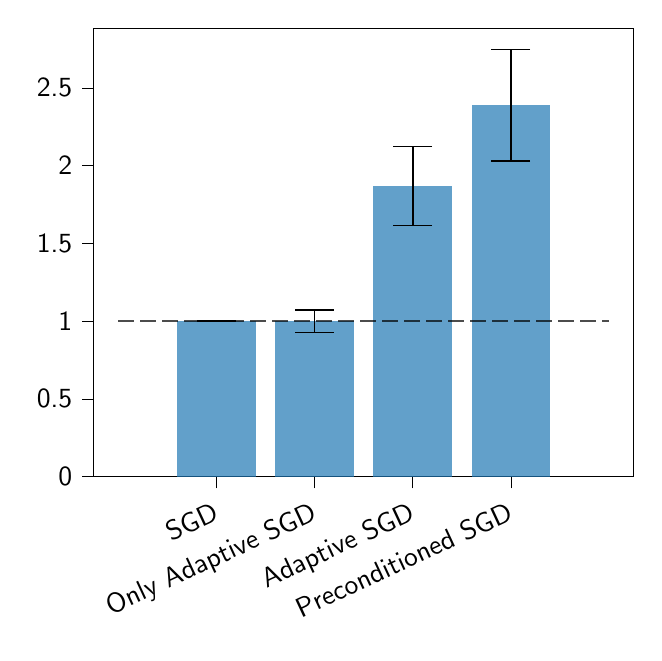
\begin{tikzpicture}

\definecolor{color0}{rgb}{0.12156862745098,0.466666666666667,0.705882352941177}

\begin{axis}[
tick align=outside,
tick pos=left,
tick pos=left,
x grid style={white!69.01960784313725!black},
xmin=-1.25, xmax=4.25,
xtick style={color=black},
xtick={0,1,2,3},
xticklabel style = {anchor = north east},
xticklabel style = {rotate=25.0},
xticklabels={SGD,Only Adaptive SGD,Adaptive SGD,Preconditioned SGD},
y grid style={white!69.01960784313725!black},
ymin=0, ymax=2.88335323873322,
ytick style={color=black}
]
\draw[fill=color0,draw opacity=0,fill opacity=0.7] (axis cs:-0.4,0) rectangle (axis cs:0.4,1);
\draw[fill=color0,draw opacity=0,fill opacity=0.7] (axis cs:0.6,0) rectangle (axis cs:1.4,0.998138761408857);
\draw[fill=color0,draw opacity=0,fill opacity=0.7] (axis cs:1.6,0) rectangle (axis cs:2.4,1.86919536286069);
\draw[fill=color0,draw opacity=0,fill opacity=0.7] (axis cs:2.6,0) rectangle (axis cs:3.4,2.38745288199299);
\path [draw=black, semithick]
(axis cs:0,1)
--(axis cs:0,1);

\path [draw=black, semithick]
(axis cs:1,0.925706236676787)
--(axis cs:1,1.07057128614093);

\path [draw=black, semithick]
(axis cs:2,1.61495128884284)
--(axis cs:2,2.12343943687854);

\path [draw=black, semithick]
(axis cs:3,2.02885506043054)
--(axis cs:3,2.74605070355544);

\path [draw=black, draw opacity=0.7, semithick, dash pattern=on 5.550000000000001pt off 2.4000000000000004pt]
(axis cs:-1,1)
--(axis cs:4,1);

\addplot [semithick, black, mark=-, mark size=7, mark options={solid}, only marks]
table {%
0 1
1 0.925706236676787
2 1.61495128884284
3 2.02885506043054
};
\addplot [semithick, black, mark=-, mark size=7, mark options={solid}, only marks]
table {%
0 1
1 1.07057128614093
2 2.12343943687854
3 2.74605070355544
};
\end{axis}

\end{tikzpicture}
\end{frame}

%\begin{frame}{Stability depending on initialization}
%%TODO Do I want to keep this? & include figure
%\end{frame}

\begin{frame}{Learning Rate Sensitivity}{vs SGD}
\centering
% This file was created by tikzplotlib v0.8.2.
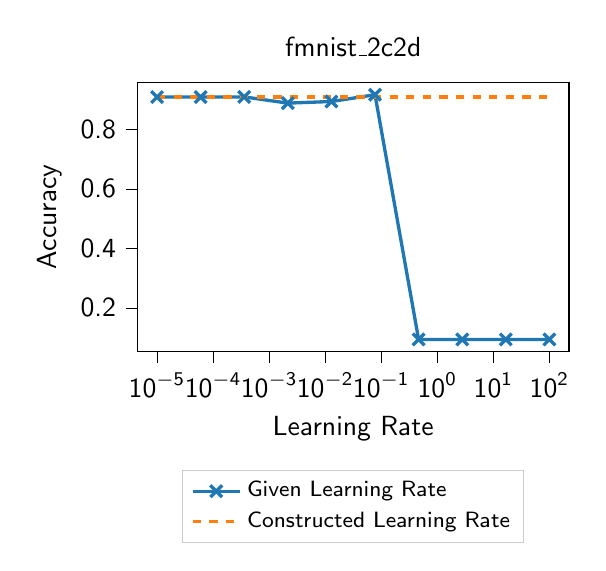
\begin{tikzpicture}

\definecolor{color0}{rgb}{0.12156862745098,0.466666666666667,0.705882352941177}
\definecolor{color1}{rgb}{1,0.498039215686275,0.0549019607843137}

\begin{axis}[
height=5cm,
legend cell align={left},
legend style={at={(0.03,0.03)}, anchor=south west, draw=white!80.0!black},
legend style={font=\footnotesize, at={(0.5 ,0)}, yshift=-1.5cm,anchor=north,nodes=right},
log basis x={10},
tick align=outside,
tick pos=left,
tick pos=left,
title={fmnist\_2c2d},
width=\figurewidth + 1cm,
x grid style={white!69.01960784313725!black},
xlabel={Learning Rate},
xmin=4.46683592150963e-06, xmax=223.872113856834,
xmode=log,
xtick style={color=black},
xtick={1e-07,1e-06,1e-05,0.0001,0.001,0.01,0.1,1,10,100,1000,10000},
xticklabels={\(\displaystyle {10^{-7}}\),\(\displaystyle {10^{-6}}\),\(\displaystyle {10^{-5}}\),\(\displaystyle {10^{-4}}\),\(\displaystyle {10^{-3}}\),\(\displaystyle {10^{-2}}\),\(\displaystyle {10^{-1}}\),\(\displaystyle {10^{0}}\),\(\displaystyle {10^{1}}\),\(\displaystyle {10^{2}}\),\(\displaystyle {10^{3}}\),\(\displaystyle {10^{4}}\)},
y grid style={white!69.01960784313725!black},
ylabel={Accuracy},
ymin=0.0525090144230769, ymax=0.957607171474359,
ytick style={color=black},
ytick={0,0.2,0.4,0.6,0.8,1},
yticklabels={0.0,0.2,0.4,0.6,0.8,1.0}
]
\addplot [very thick, color0, mark=x, mark size=3, mark options={solid}]
table {%
0 0.906850961538462
1e-05 0.908653846153846
5.99484250318941e-05 0.908553685897436
0.000359381366380463 0.909154647435897
0.00215443469003188 0.888221153846154
0.0129154966501488 0.893729967948718
0.0774263682681127 0.916466346153846
0.464158883361278 0.0936498397435897
2.78255940220713 0.0936498397435897
16.6810053720006 0.0936498397435897
100 0.0936498397435897
};
\addlegendentry{Given Learning Rate}
\addplot [very thick, color1, dashed]
table {%
1e-05 0.908844150641026
100 0.908844150641026
};
\addlegendentry{Constructed Learning Rate}
\end{axis}

\end{tikzpicture}
\end{frame}

\begin{frame}{Conclusion/Final Remarks}{}

\end{frame}


\blackslidetext{end of presentation}


\end{document}